% Use the temporary template.
\documentclass[12pt]{aiaa-pretty}

\usepackage{amssymb,amsmath}
\usepackage{graphicx,float}
\usepackage{lettrine}
\usepackage{wasysym} % For double surface close integrals

%\usepackage{setspace} 
%\doublespacing
\usepackage{subfigure} %For side-by-side figures
\usepackage{epstopdf} %To read *.eps Files
\usepackage{multirow}

\usepackage[T1]{fontenc}
\usepackage[utf8]{inputenc}
%\usepackage{authblk}

% FOR TABLES
\usepackage{multirow}
\usepackage{array}
\newcolumntype{L}[1]{>{\raggedright\let\newline\\\arraybackslash\hspace{0pt}}m{#1}}
\newcolumntype{C}[1]{>{\centering\let\newline\\\arraybackslash\hspace{0pt}}m{#1}}
\newcolumntype{R}[1]{>{\raggedleft\let\newline\\\arraybackslash\hspace{0pt}}m{#1}}

\usepackage[linewidth=1pt]{mdframed}
\usepackage{lipsum}

% Author information
\author[Gobal, Kohler, and Grandhi]{ %
Koorosh Gobal\thanks{Graduate Research Assistant, Department of Mechanical and Materials Engineering, AIAA Student Member; gobal.2@wright.edu.},
Ramana V. Grandhi\thanks{Distinguished Research Professor, AIAA Fellow.}\\
\textit{Wright State University, Dayton, Ohio 45324}
\\
and 
\\
Christopher M. Koehler\thanks{Research Engineer, Multidisciplinary Sciences and Technology Center.}\\
\textit{Air Force Research Laboratory, Wright-Patterson Air Force Base, Ohio 45433}}


% Title
\title{A Robust Analytical Sensitivity Analysis for Coupled Aero-Structural Systems}

% Abstract
 \abstract{In this research, a continuum sensitivity formulation for the shape sensitivity analysis of a coupled fluid-structure system is derived. The flow field is modeled using incompressible Navier-Stokes equations and the solid domain is represented as a linear elastic model. The conventional approach to this problem is based on a body-conformal grid to represent the solid boundaries. However, these methods fail for complex shapes and/or large deformations of the solid region. This issue can be addressed by using the immersed boundary method, where additional force terms are added to the governing equations to represent the solid boundaries. Using this approach, significant computational saving is achieved by two means: 1) Highly efficient solvers can be utilized on Cartesian grids, and 2) Mesh deformation is not necessary. The sensitivity analysis consists of differentiating the continuum form of the governing equations. In this approach the sensitivity and governing equations use the same differential operators. Therefore same solver is utilized for both systems of equations. Proposed methodology is used to solve a 2D flow over a cylinder and a simplified aeroelastic wing model. The sensitivity of flow field around and on the cylinder, airfoil lift, and wing structural responses are calculated with respect to shape parameters. High-fidelity computational fluid dynamics (CFD) is used to solve the flow problem and wing structure is represented with a finite element model. The sensitivity results are verified using the complex step method where a good agreement is realized.}


% Begin the document
\begin{document}
% Insert the title.
\maketitle
% ==========================================================================================
\section{Introduction}
Fluid-structure interaction (FSI) plays prominent roles in many scientific and engineering fields, yet a comprehensive study of such problems remains a challenge due to their strong coupling, nonlinearity and complexity in simulation of high-fidelity physics. For most FSI problems, analytical solutions are impossible to obtain, whereas physical experiments are limited in scope. Thus, to investigate the physics involved in the interaction between fluids and structures, numerical simulations are often employed. These techniques are based on coupled computational fluid dynamics (CFD) approaches for solving the flow problem and finite element analysis (FEA) for calculating the structural responses. However, generating and keeping the quality of the CFD mesh as the structure deforms due to aerodynamic loads can become a major issue. Moreover, with the growing interest in Multidisiplinary Design Optimization (MDO) techniques for fluid-structural problems, numerical sensitivity analysis methods, such as finite difference, has proven to be infeasible due to their inaccuracy. Successfull implementation of MDO requires an accurate and efficient method for calculating the sensitivities.

Formulation of the analytical sensitivity methods requires derivation of analytic sensitivity equations. These equations are obtained by differentiating the governing equations with respect to design variables such as shape of the boundaries. Among various available methods, the discrete analytic sensitivity is a popular approach. This method is based on differentiating the discretized system of governing equations \cite{martins2013review}. In order to differentiate the discretized system of equations, it is necessary to modify the source-code of the black-box CFD/FEA solvers \cite{cross2014local}. This might not be possible due to solver's source codes availability. Moreover, the discrete model has high costs, especially in terms of operation costs and memory requirements \cite{peter2010numerical}.

The Continuum Sensitivity Analysis (CSA), involves solving a set of partial differential equations named the continuum sensitivity equations (CSEs) to calculate analytical sensitivities. CSA has several computational efficiencies that other sensitivity formulations lack. Aurora and Haug \cite{Arora}, and later Dems and Mroz \cite{Dems-Mroz} were among the first to introduce CSA for structural problems. Stanley and Stewart \cite{stanley2002design} applied CSA to fluid mechanics for aerodynamic design. Pelletier and Etienne applied CSA to several fluid-structure interaction (FSI) problems \cite{etienne2005general} focused mainly on sensitivities of fluid flow parameters near the structure. Liu and Canfield have employed CSA for shape optimization of nonlinear structures subject to an aeroelastic gust response \cite{liu2013equivalence}. They used the finite element method to solve the potential flow around an airfoil and applied CSA to find the airfoil pressure coefficient sensitivity with respect to the maximum camber. In these works, body conforming grids were used to model the flow around the solid bodies. The conforming mesh methods consider the interface conditions as physical boundary conditions, which treat the interface location as part of the solution and requires meshes that conform to the interface. Owing to the movement and/or deformation of the solid structure, re-meshing (or mesh-updating) is needed as the solid boundaries move. Although conforming mesh methods have been widely used in many FSI problems, they are cumbersome, if not impossible, to apply to problems with large deformations \cite{sahin2009arbitrary}. Moreover, when performing sensitivity analysis on a deforming mesh, it is required to calculate the mesh sensitivities as well \cite{liu2013boundary}. This adds to the computational cost of calculating  sensitivities. The shortcoming of a body conforming grid generation and the additional cost of calculating mesh sensitivities motivate the current work to develop a method that does not require fluid domain mesh modification for the optimization iterations.

The non-conforming mesh methods treat the boundary location as constraints imposed on governing equations. As a result, the fluid and solid equations can be conveniently solved independently from each other on their respective grids and re-meshing is not necessary. The distinction between these two types of meshes can be observed in Figure \ref{fig:conformalVSnonconformal}, where a solid body (a sphere) is moving in a fluid domain.

%
\begin{figure}[H]
	\centering
	\subfigure[Conforming mesh, $t = t_1$]
	{
	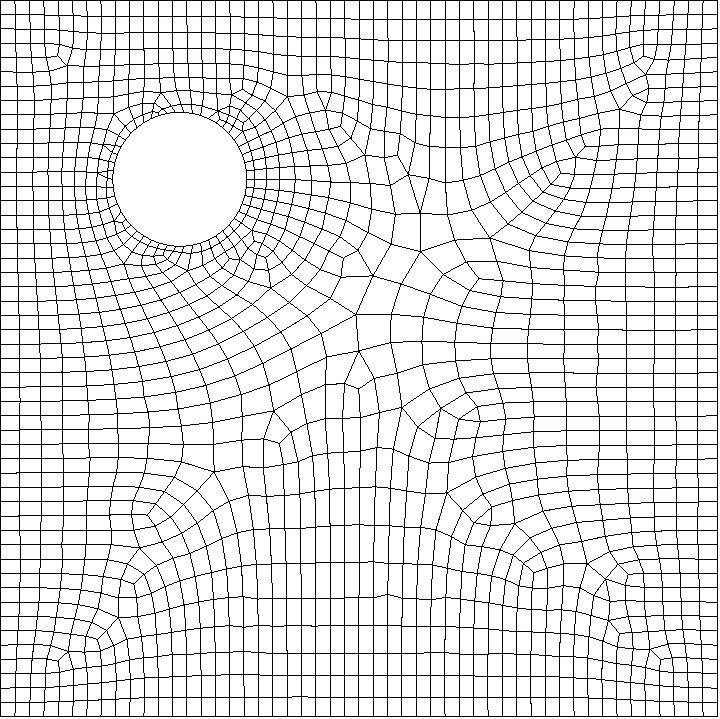
\includegraphics[height=5.0cm]{figure/conforming_t1.jpg}
	}
	\quad
	\subfigure[Conforming mesh, $t = t_2$]
	{
	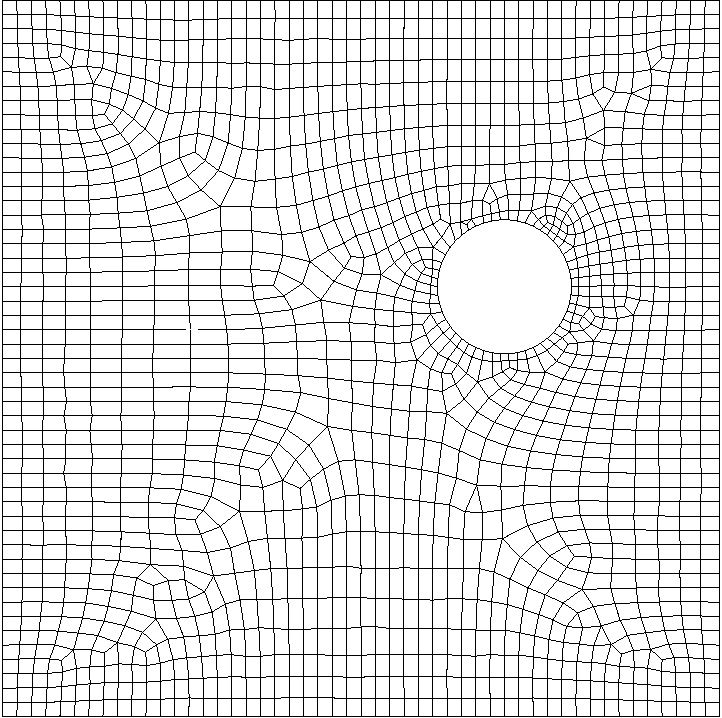
\includegraphics[height=5.0cm]{figure/conforming_t2.jpg}
	}
	\\
	\subfigure[Nonconforming mesh, $t = t_1$]
	{
	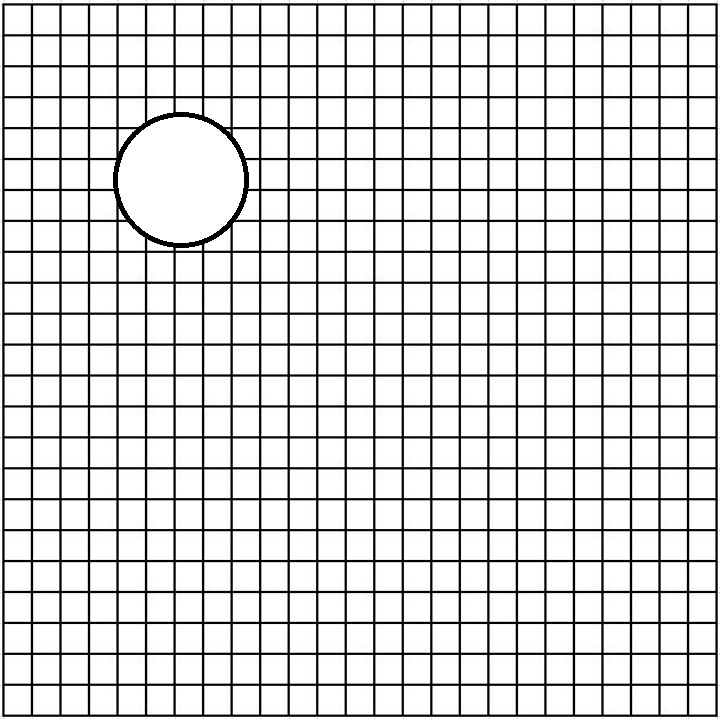
\includegraphics[height=5.0cm]{figure/nonconforming_t1.jpg}
	}
	\quad
	\subfigure[Nonconforming mesh, $t = t_2$]
	{
	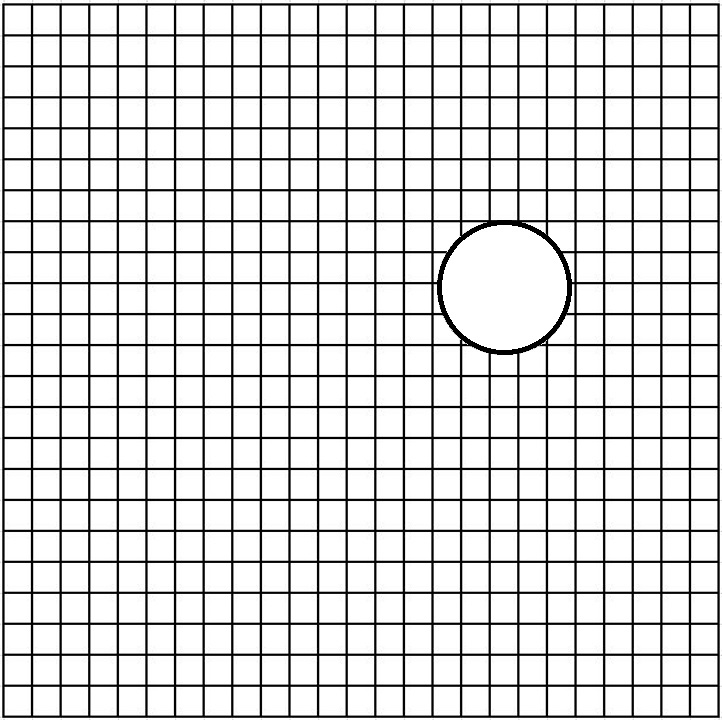
\includegraphics[height=5.0cm]{figure/nonconforming_t2.jpg}
	}
	\caption{Example of conforming and nonconforming meshes.}
	\label{fig:conformalVSnonconformal}
\end{figure}
%

Most non-body conforming mesh techniques are based upon the framework of the Immersed Boundary (IB) methods where a numerically efficient Cartesian grid is used for the discretization of the fluid domain. The effect of solid boundaries can be handled in the continuous domain, i.e. before discretization, or by altering the linear system resulting from discretization in time and space, which is termed discrete forcing \cite{mittal2005immersed}. The advantage of IB method is that it eliminates the inefficient task of grid generation which can be costly for problems involving moving and deforming immersed boundaries. In the immersed boundary method, the boundary of an immersed solid is tracked by Lagrangian markers that are convected by a fluid. Numerically, the communication between the solid and the fluid is obtained by spreading singular forces from the Lagrangian markers to nearby Cartesian grid nodes and interpolating the velocity from nearby Cartesian grid nodes to the Lagrangian markers with the use of discrete Dirac $\delta$ functions.

In recent years, the immersed boundary method has been applied to multiple FSI problems. Choi et al. calculated the surface pressure coefficients for high Reynolds number flow around an NACA0012 airfoil \cite{choi2007immersed}. Fadlun et al. investigated the capability of this method to simulate high-Reynolds number turbulent flows in complex geometries. They chose an axisymmetric piston-cylinder assembly with a fixed central valve for this purpose \cite{fadlun2000combined}. Vanella et al. tested the accuracy of immersed boundary method for the case of two falling plates \cite{vanella2010direct}. 

Most research that has been done on the immersed boundary focused on the analysis aspects of the method and the sensitivity analysis has not been extensively studied. There has been limited research on the application of immersed boundary method for optimization of the internal flows where the penalization technique was used to optimize the shape of the channels for fluid flow \cite{challis2009level, kreissl2012levelset}; however, the developed methodology is only applicable to low Reynolds number flows and does not provide good accuracies near the solid boundaries.

In this research, we use the continuum sensitivity analysis to calculate the sensitivity of coupled FSI problems to shape parameters, where the flow is modeled using steady, laminar, incompressible Navier-Stokes equations. We used high fidelity CFD simulation to solve the flow equations and linear FEA model for the structural analysis. The fluid-solid interaction is modeled using the continuum immersed boundary method which is capable of sharp representation of the solid boundaries. The traditional immersed boundary method uses a discrete Dirac function for transferring data between domains. This is not applicable when using continuum sensitivity analysis since the governing equations need to be continuously differentiable. Therefore, a continuous regularized delta function is developed to satisfy this need. The methodology is applied to flow over a cylinder and a wing model for a coupled aero-structure representation. The analytical sensitivities of flow and structural response are calculated with respect to shape parameters with CSA and verified using the complex step method.

% ==========================================================================================
\section{Numerical Approach}
% -.-.-.-.-.-.-.-.-.-.-.-.-.-.-.-.-.-.-.-.-.-.-.-.-.-.-.-.-.-.-.-.-.-.-.-.-.-.-.-.-.-.-.-.-
\subsection{Immersed Boundary Formulation}
Viscous and incompressible flow in a Cartesian square domain $\Omega$ containing an immersed boundary, as shown in Figure \eqref{fig:immersedBoundary}, is modelled by the Navier-Stokes equations:

%
\begin{subequations}\label{eq:NS}
\begin{equation}
	\rho \left[
	\frac{\partial \vec{V}}{\partial t} + 
	\left( \vec{V} \cdot \nabla \right) \vec{V}
	\right] = 
	-\vec{\nabla} P + \mu \nabla^2 \vec{V} + \vec{F}
\end{equation}
\begin{equation}
	\vec{\nabla} \cdot \vec{V} = 0
\end{equation}
\end{subequations}
%

where $\rho$ is density; $\mu$ is dynamic viscosity; $\vec{V}$ is fluid velocity; and $P$ is the fluid pressure. The forcing function, $\vec{F}$ is given by

%
\begin{equation}\label{eq:forceAtEulerian}
	\vec{F}(\vec{x}, t) = \int_\Omega \vec{f} (\vec{x}_k, t) \delta(\vec{x} - \vec{x}_k) d\vec{x}_k
\end{equation}
%

where $\delta(\vec{x} - \vec{x}_k)$ is a Dirac delta function; $\vec{x}_k$ are the locations of Lagrangian points placed over the immersed boundary; $\vec{f}(\vec{x}_k)$ is the Lagrangian force density; and $\vec{F}(\vec{x})$ is the Eulerian force that has non-zero values only over the immersed boundary. The Lagrangian force terms are calculated using virtual boundary formulation proposed by Goldstein \cite{goldstein1993modeling}. The main idea of this method is to treat the embedded boundary by adding a force field to the fluid, in such away that the fluid takes the same velocity as the solid surface. Since the force field is not known a priori, it must be calculated in a feedback way as shown in Equation \eqref{eq:forcingFunction}. This model involves two imposed constants, $\alpha$ and $\beta$, which are chosen to be both negative and large enough in magnitude to force the fluid velocity to the interface velocity. The feedback forcing function $\vec{f}(\vec{x}_k, t)$ is given as

%
\begin{equation}\label{eq:forcingFunction}
	\vec{f}\left( \vec{x}_k, t \right) = 
	\alpha \int_0^t \left[ \vec{u}\left( \vec{x}_k, t \right) - \vec{U}\left( \vec{x}_k, t \right) \right]dt + 
	\beta \left[ \vec{u}\left( \vec{x}_k, t \right) - \vec{U}\left( \vec{x}_k, t \right) \right]
\end{equation}
%

where $\vec{u}\left( \vec{x}_k, t \right)$ is the velocity value from the Eulerian analysis calculated at the Lagrangian nodes. $\vec{U}\left( \vec{x}_k, t \right)$ is the velocity at the corresponding Lagrangian nodes, $\vec{x}_k$. For the case of a no-slip boundary condition ($\vec{U}\left( \vec{x}_k, t \right) = 0 $) the forcing function in Equation \eqref{eq:forcingFunction} tries to bring the velocity to zero on the boundary. $\vec{u}\left( \vec{x}_k, t \right)$ is calculated from its neighbouring Eulerian nodes by using the same delta function used in Equation \eqref{eq:forceAtEulerian}.

%
\begin{equation}\label{eq:velocityAtLagrangian}
	\vec{u}(\vec{x}_k, t) = \int_\Omega \vec{u} (\vec{x}, t) \delta(\vec{x} - \vec{x}_k) d\vec{x}
\end{equation}
%

%
\begin{figure}[H]
	\centering
	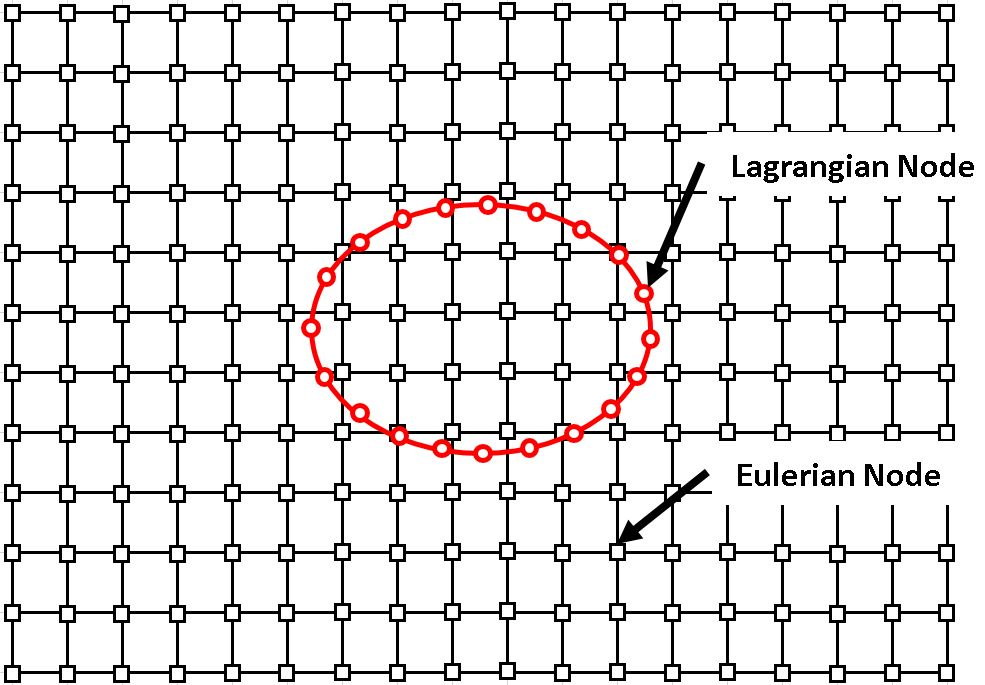
\includegraphics[height=6.0cm]{figure/immerdBoundary.jpg}
	\caption{Immersed boundary illustration}
	\label{fig:immersedBoundary}
\end{figure}
%

Shin et al. investigated the stability of virtual boundary formulation for various types of regularized delta functions \cite{shin2008assessment}. These functions have different bandwidths which correspond to the number of Eulerian points where the effect of forcing function is distributed however they are not continuously differentiable. In continuum sensitivity analysis approach, the governing equations are differentiated to get the sensitivity equations. Therefore, it is required for the delta functions to have a continuous derivative. We propose the following Regularized Delta (RD) function formulation that satisfies this need.

%
\begin{equation}\label{eq:heavisideFunction}
	\delta_h(\vec{x}) = \frac{1}{h^3} \phi \left( \frac{x - x_k}{h} \right)
									 \phi \left( \frac{y - y_k}{h} \right)
									 \phi \left( \frac{z - z_k}{h} \right)
\end{equation}
%

where $h$ is the distance between the Eulerian nodes. $\phi$ is defined as:

%
\begin{equation}\label{eq:continuousDeltaFunction}
	\phi(r) = \dfrac{1}{\eta} \left( \dfrac{-\tanh^{2}{\left (\dfrac{r}{\eta} \right )} + 1}{2} \right)
	               \quad , \quad 
	               r = \frac{x - x_k}{h}
\end{equation}
%

For the RD function, the free parameter ($\eta$) is calculated by selecting how fast the RD function decays when moving further from its symmetry axis. The free parameter for the RD function is defined in Equation \eqref{eq:etaGuideForRDfunction}.

\begin{equation}\label{eq:etaGuideForRDfunction}
    \eta = \frac{R}{\tanh^{-1} (\sqrt{1 - p})}
\end{equation}

RD function drops to $p$ percentage of its value at the symmetry axis at distance $R$. For example, for the RD function value to drop 99 percent ($p = 0.99$) within 0.01 ($R = 0.01$) of the symmetry axis of the RD function, the $\eta$ value is calculated as $0.0033$ based on Equation \eqref{eq:etaGuideForRDfunction}.

%
\begin{figure}[H]
	\centering
	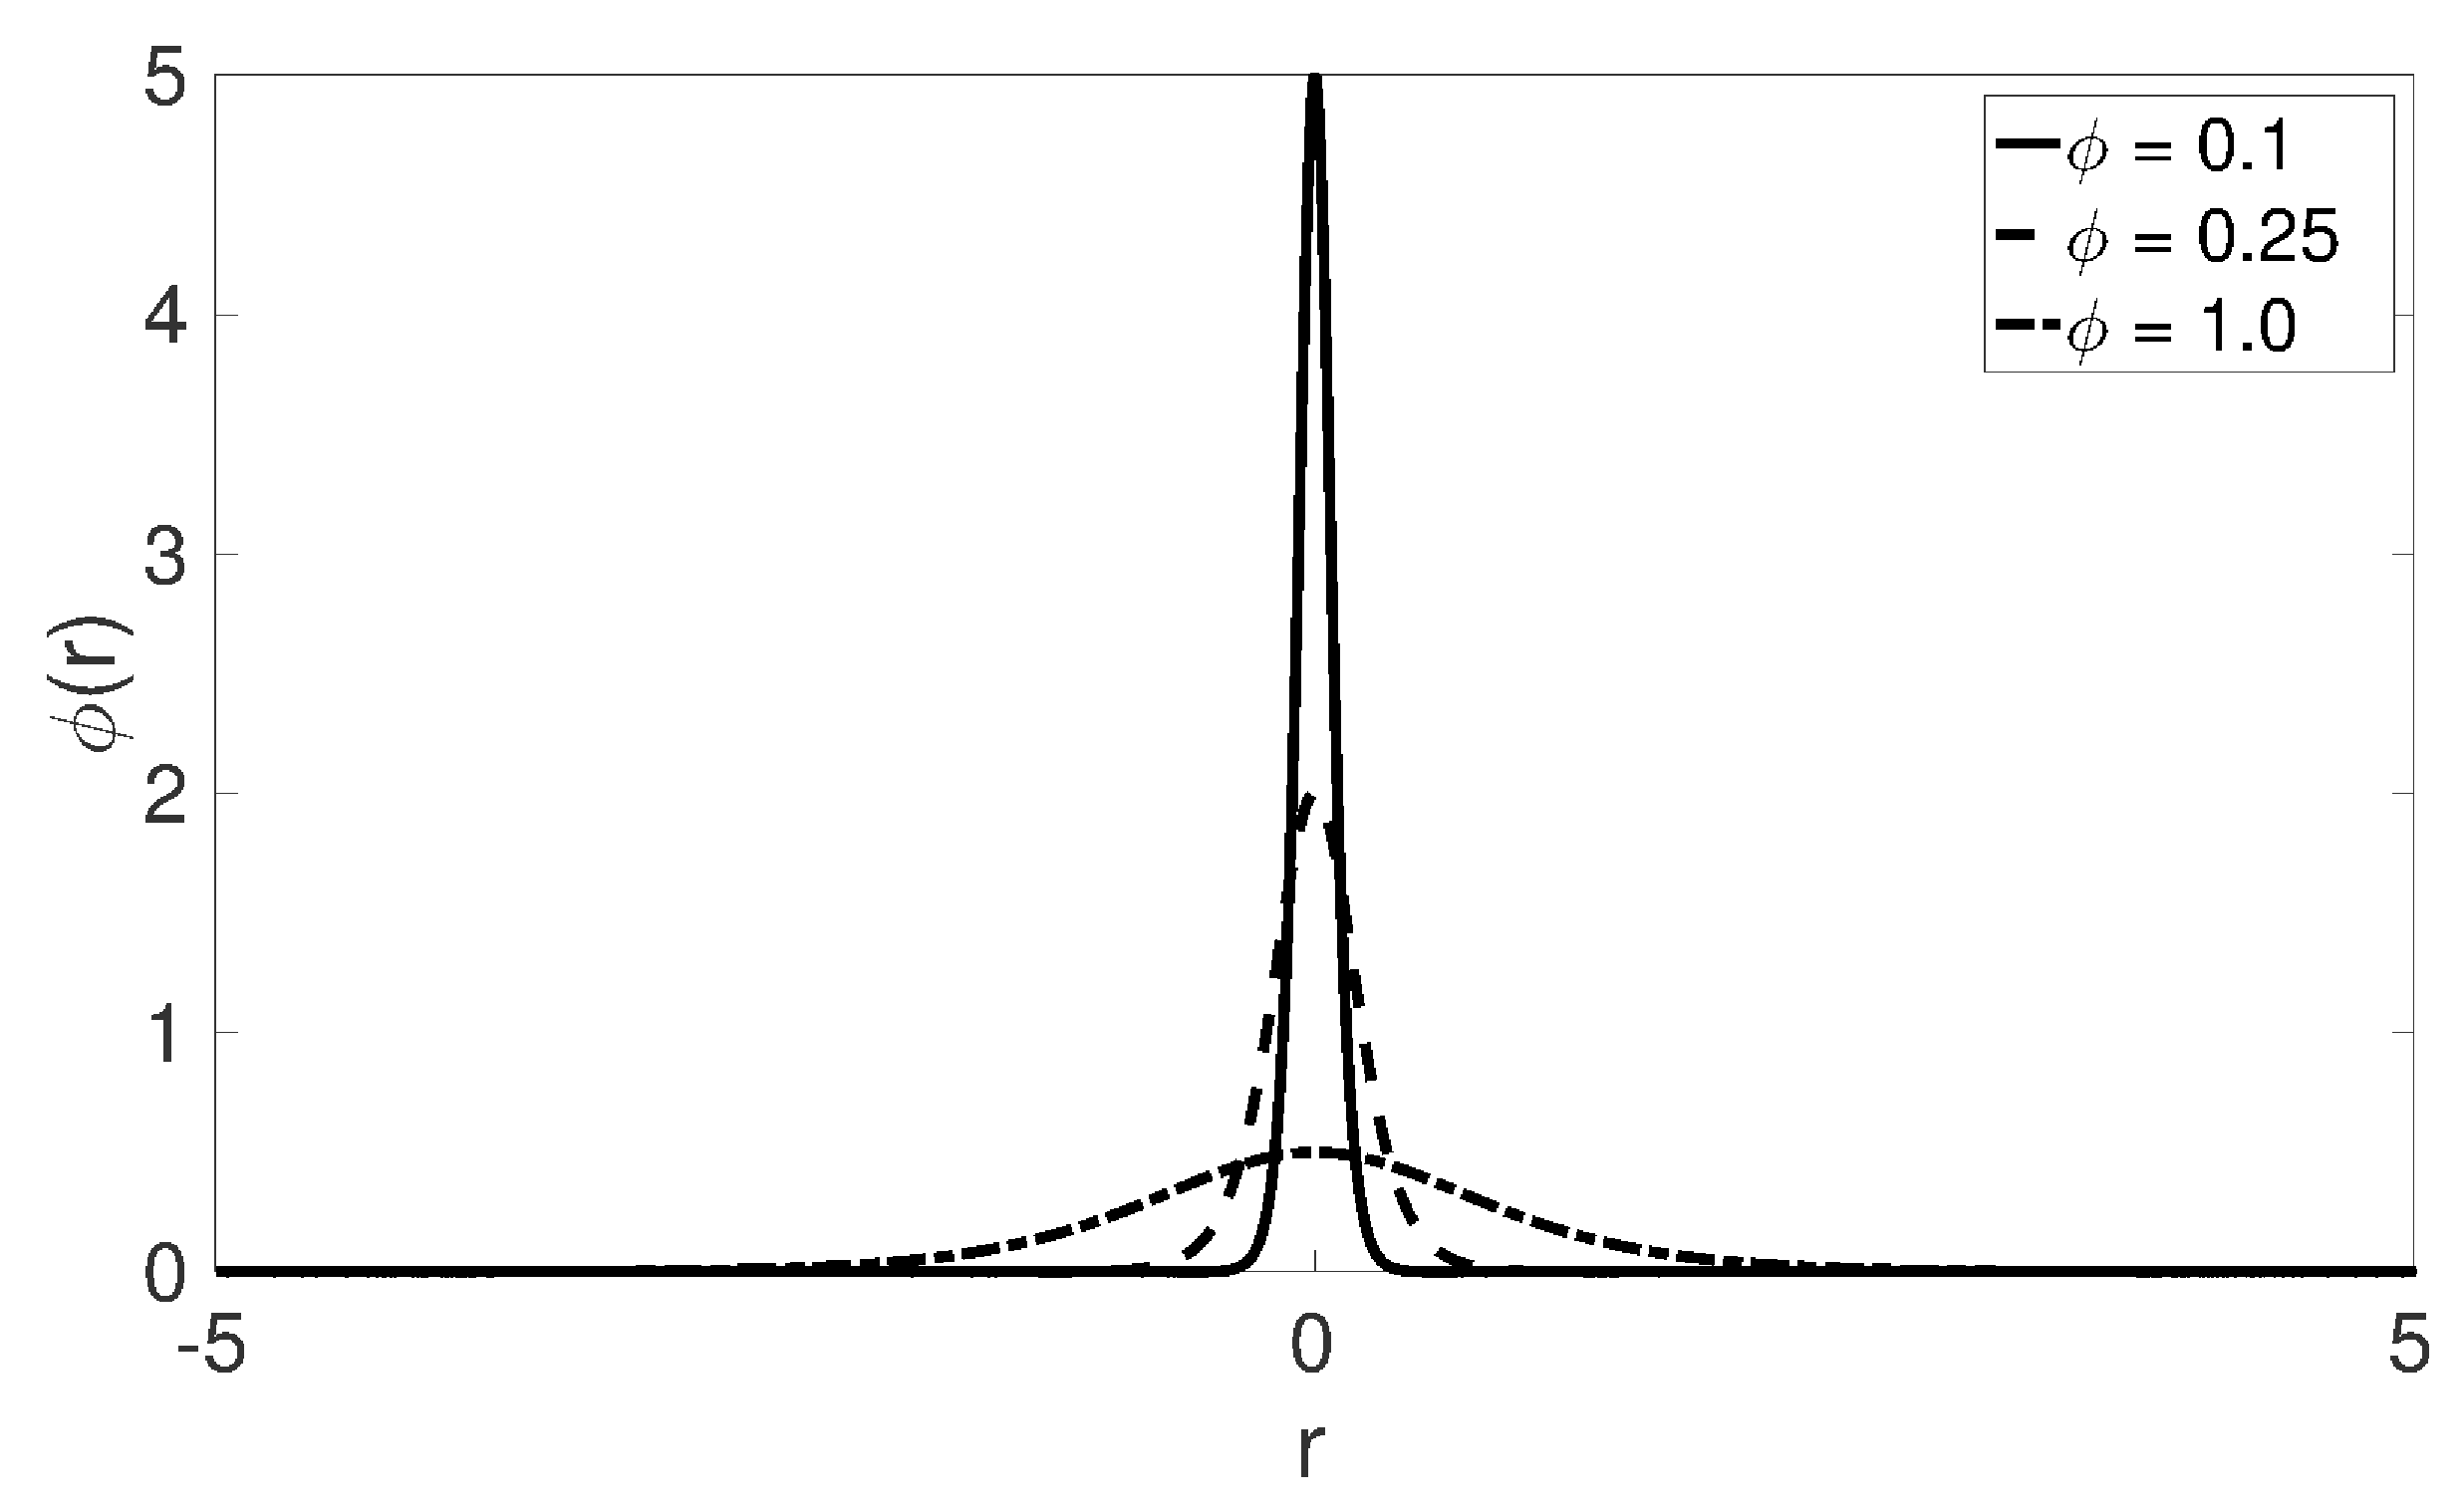
\includegraphics[height=6.0cm]{figure/heaviside_comparison.eps}
	\caption{Comparison between different delta function formulations.}
	\label{fig:heavisideComparison}
\end{figure}
%

Finally, the forcing function, $\vec{F}(\vec{x})$, can be written by combining equations \eqref{eq:forceAtEulerian}, \eqref{eq:forcingFunction}, and \eqref{eq:velocityAtLagrangian}.

%
\begin{equation}
\begin{aligned}\label{eq:forceAtEulerianFinal}
	\vec{F}(\vec{x}, t) = 
	\int_\Omega 
	&\left\{
 	\alpha \int_0^t
	\left[
	\int_\Omega \vec{u} (\vec{x}, t) \delta(\vec{x} - \vec{x}_k) d\vec{x} - \vec{U}\left( \vec{x}_k, t \right)
	\right]dt + \right. \\
	&\left.
	\beta \left[
	\int_\Omega \vec{u} (\vec{x}, t) \delta(\vec{x} - \vec{x}_k) d\vec{x} - \vec{U}\left( \vec{x}_k, t \right)
	\right]
	\right\} \delta(\vec{x} - \vec{x}_k) d\vec{x}_k
\end{aligned}
\end{equation}
%

In Equation \eqref{eq:forceAtEulerianFinal}, the integrals on the domain, $\Omega$, transfer the data between the Lagrangian and Eulerian domains. The inner integrals, map the velocities from Eulerian to Lagrangian nodes to calculate the force at Lagrangian node, $\vec{f}\left( \vec{x}, t \right)$. The outer integral maps the forcing function from the Lagrangian to Eulerian nodes where the governing equations are solved (Figure \ref{fig:mappingDataE2L}).

%
\begin{figure}[H]
	\centering
	\subfigure[Velocity calculation at the Lagrangian nodes.]
	{
	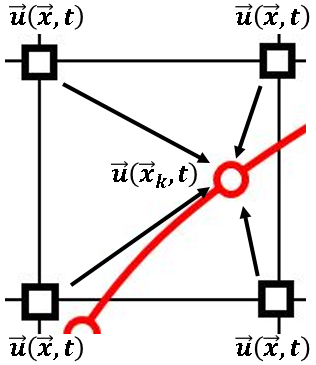
\includegraphics[height=5.0cm]{figure/mapping_1.png}
	}
	\quad
	\subfigure[Forcing function evaluation.]
	{
	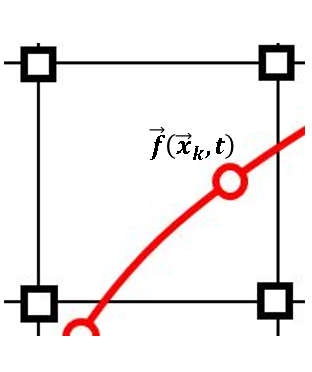
\includegraphics[height=5.0cm]{figure/mapping_2.png}
	}
	\quad
	\subfigure[Forcing function transfer to the Eulerian nodes.]
	{
	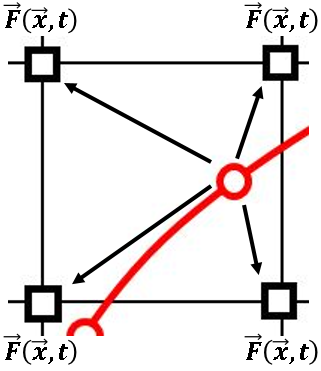
\includegraphics[height=5.0cm]{figure/mapping_3.png}
	}
	\caption{Data transfer between Eulerian and Lagrangian nodes.}
	\label{fig:mappingDataE2L}
\end{figure}
%

% -.-.-.-.-.-.-.-.-.-.-.-.-.-.-.-.-.-.-.-.-.-.-.-.-.-.-.-.-.-.-.-.-.-.-.-.-.-.-.-.-.-.-.-.-
\subsection{Analytic Sensitivity Formulation}
Figure \ref{fig:domain} represents the domain, $\Omega$, in the Cartesian space. This domain is the union of the solid, $\Omega_s$, and fluid, $\Omega_f$, domains where the Navier-Stokes equations are solved. The far field boundary conditions which are defined on the sides of this domain, $\Gamma$, are not affected by the design variables. By using this approach, the boundaries of the solid domain are added to the fluid's governing equations as mentioned in the previous section.

%
\begin{figure}[H]
	\centering
	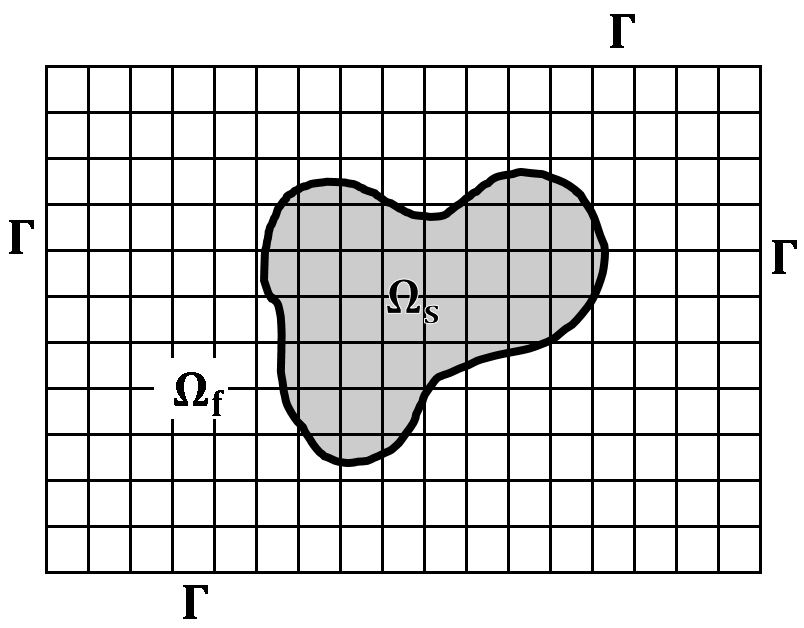
\includegraphics[height=6.0cm]{figure/domain.jpg}
	\caption{Computational domain, $\Omega = \Omega_f \cup \Omega_s$, with boundary of $\Gamma$}
	\label{fig:domain}
\end{figure}
%

The governing equation and boundary conditions are written in the general form as

%
\begin{subequations}\label{eq:generalFormForGE}
\begin{equation}
	A(\vec{u}, \vec{b}) = f(\vec{x}, t; \vec{b}) \quad \text{on} \quad \Omega
\end{equation}
\begin{equation}
	B(\vec{u}, \vec{b}) = g(\vec{x}, t; \vec{b}) \quad \text{on} \quad \Gamma
\end{equation}
\end{subequations}
%
Here $A$ and $B$ are the differential operators for the governing equations and boundary conditions respectively. $\vec{u}$ is the vector of response variables, that could be displacements in structural mechanics or velocities and pressure in fluid dynamics. The vectors $\vec{x}$ and $\vec{b}$ contain spatial coordinates and design variables, respectively. The total sensitivity of the response variable $\vec{u}$ to the $i^\text{th}$ design variable $b_i$ is calculated as

%
\begin{equation}
	\frac{D\vec{u}}{Db_i	} = \frac{\partial \vec{u}}{\partial b_i} + 
	                        \frac{\partial \vec{u}}{\partial \vec{x}} \cdot \frac{\partial \vec{x}}{\partial b_i}
\end{equation}
%

This material derivative consists of the local design derivative, $\partial \vec{u} / \partial b_i$, plus a convective term, $\partial \vec{u} / \partial \vec{x} \cdot \partial \vec{x} / \partial b_i$. The local design derivative is a measure of how much the response at a point changes due to change in the design parameters. The convective term tracks the movement of the material point when the spatial coordinates change with the design variable. The geometric domain can be a function of the design variables in the case of body conformal meshes (Figure \ref{fig:conformalVSnonconformal}). However, non-body conformal meshes will not change as the design parameter vary. Therefore, the convective term is equal to zero \cite{gobal2014continuum}. Thus the local and total forms of the sensitivities are equal.

The local sensitivity equations are derived by partial differentiation of Equation \eqref{eq:NS} along with its boundary conditions. The differentiation to $i^\text{th}$ design variable, $b_i$, yields the tangent form of the governing equations:

%
\begin{subequations}\label{eq:NSforSA}
\begin{equation}
	\rho \left[
	\frac{\partial \vec{V^\prime}}{\partial t} + 
	\left( \vec{V^\prime} \cdot \nabla \right) \vec{V} + 
	\left( \vec{V} \cdot \nabla \right) \vec{V^\prime}
	\right] = 
	-\vec{\nabla} P^\prime + \mu \nabla^2 \vec{V^\prime} + \vec{F^\prime}
\end{equation}
\begin{equation}
	\vec{\nabla} \cdot \vec{V^\prime} = 0
\end{equation}
\end{subequations}
%

In the above equation, $\vec{V^\prime}$ and $P^\prime$ are the local sensitivities of the velocity and pressure to $i$-th design variable, $b_i$, respectively. $\vec{V}$ is calculated from the solution of the governing equation \eqref{eq:NS}. Comparing equations \eqref{eq:NS} and \eqref{eq:NSforSA}, we can see that the form of the governing and sensitivity equations are the same. Therefore, we can use the same solver for solving both of these equations. This is not possible when using the discrete formulation for the sensitivity analysis.

The effect of boundary movement is introduced in Equation \eqref{eq:NSforSA} through $\vec{F^\prime}$, more specifically through the derivative of the regularized delta function with respect to design variable, $b_i$. The derivative of the forcing function is derived as

%
\begin{equation}
\begin{aligned}\label{eq:forceingFunctionDerivative}
	\vec{F^\prime}(\vec{x}, t) = 
	\int_\Omega 
	&\left\{
 	\alpha \int_0^t
	\left[
	\int_\Omega \vec{u^\prime} (\vec{x}, t) \delta(\vec{x} - \vec{x}_k) d\vec{x} - 
	\int_\Omega \vec{u} (\vec{x}, t) \frac{\partial \delta(\vec{x} - \vec{x}_k)}{\partial \vec{x}_k} \frac{\partial \vec{x}_k}{\partial b_i} d\vec{x}
	\right]dt + \right. \\
	&\left.
	\quad \beta
	\left[
	\int_\Omega \vec{u^\prime} (\vec{x}, t) \delta(\vec{x} - \vec{x}_k) d\vec{x} - 
	\int_\Omega \vec{u} (\vec{x}, t) \frac{\partial \delta(\vec{x} - \vec{x}_k)}{\partial \vec{x}_k} \frac{\partial \vec{x}_k}{\partial b_i} d\vec{x}
	\right]
	\right\} \delta(\vec{x} - \vec{x}_k) d\vec{x}_k + \\
	\int_\Omega 
	&\left\{
 	\alpha \int_0^t
	\left[
	\int_\Omega \vec{u} (\vec{x}, t) \delta(\vec{x} - \vec{x}_k) d\vec{x} - \vec{U}\left( \vec{x}_k, t \right)
	\right]dt + \right. \\
	&\left.
	\quad \beta \left[
	\int_\Omega \vec{u} (\vec{x}, t) \delta(\vec{x} - \vec{x}_k) d\vec{x} - \vec{U}\left( \vec{x}_k, t \right)
	\right]
	\right\} \frac{\partial \delta(\vec{x} - \vec{x}_k)}{\partial \vec{x}_k} \frac{\partial \vec{x}_k}{\partial b_i} d\vec{x}_k
\end{aligned}
\end{equation}
%
where $\vec{u^\prime}\left( \vec{x}, t \right)$ is the sensitivity of the velocity to design parameter, $b_i$. The chain rule was used to differentiate the regularized delta function with the design variable, $b_i$. The shape of the design variable only affects the location of the Lagrangian points. The derivative of the Lagrangian nodes, $\vec{x}_k$, with respect to $b_i$ can be easily calculated by the problem definition since the dependency of the shape of the domain (Lagrangian nodes) and design variables are known. The derivative of the regularized delta function to the Lagrangian node, $x_k$, is calculated analytically by differentiating Equation \eqref{eq:continuousDeltaFunction}. This results in a system of differential equations for the sensitivity response of the system. This method has a significant advantage over the conventional body conforming approaches, since there is no need to calculate the sensitivity of the boundary condition or computational mesh with respect to the design variable.

% ==========================================================================================
\section{Demonstration Results}
In this section, we apply the continuum sensitivity analysis to shape sensitivity analysis of the flow response. In these problems, the immersed solid boundaries are modelled using the immersed boundary approach as discussed in the previous section. We consider two demonstration problems: i) the flow over a cylinder ii) one-way fluid-structure coupling of the flow over an airfoil mounted on a flexible sting. The flow is modelled as an incompressible, viscous, and laminar flow. The governing equations are discretized as in Equation \eqref{eq:NSdiscretized}.

%
\begin{subequations}\label{eq:NSdiscretized}
\begin{equation}
	\frac{\vec{V}^{n+1} - \vec{V}^n}{\Delta t} + 
	\left( \frac{3}{2} N\vec{V}^n - \frac{1}{2} N\vec{V}^{n-1} \right) = 
	-G p^{n + 1/2} + 
	\frac{1}{2Re} \left( L \vec{V}^{n+1} + L \vec{V}^n \right) + 
	\vec{F}^n
\end{equation}
\begin{equation}
	D \vec{V}^{n+1} = 0
\end{equation}
\end{subequations}
%

In this equation, $\vec{V}$ is the velocity vector, $p$ is the pressure, $Re$ is the Reynolds number, $\vec{F}$ is the forcing function applied to enforce the no-slip boundary condition along the immersed boundary, $N$ is the discrete convective operator, $G$ is the discrete gradient operator, $L$ is the discrete Laplacian operator, and $D$ is the discrete divergence operator. Here, $n$ denotes the $n^\text{th}$ time step and $\Delta t$ denotes the time increment. The discrete spatial operators $N$, $G$, $L$, and $D$ are evaluated using second-order accurate central finite-differences. The numerical method is based on the Navier-Stokes solver, adopting the fractional-step method and a staggered Cartesian grid system. As shown above, the force terms are treated explicitly. The projection approach of \cite{brown2001accurate} is used to solve this coupled system of equations.

The complex step method is used to verify the sensitivity results \cite{martins2003complex}. Complex step differentiation is a technique that employs complex arithmetic to obtain the numerical value of the first derivative of a real valued analytic function of a real variable, avoiding the loss of precision inherent in traditional finite differences. The complex step derivative is calculated as follows

%
\begin{equation}\label{eq:compelxStepFormula}
	\mathcal{F}^\prime\left(u; b\right) = \frac{\text{Im}\left[ \mathcal{F}\left(u; b + ih\right) \right]}{h}
\end{equation}
%

This means that we perturb the design variable by an imaginary value of $ih$ and then look at the imaginary portion of the resulting response. Using the complex step method, we can choose a small step size for $h$ without loosing accuracy.

% -.-.-.-.-.-.-.-.-.-.-.-.-.-.-.-.-.-.-.-.-.-.-.-.-.-.-.-.-.-.-.-.-.-.-.-.-.-.-.-.-.-.-.-.-
\subsection{Flow Over a Cylinder}
The flow around a cylinder is modelled with the aforementioned methods. Sensitivity of the flow to the cylinder radius is also calculated. The domain is defined as a rectangle with length and height of 2 m and 1 m respectively, as shown in Figure \ref{fig:cylinderDomain}. The cylinder radius is selected as 0.1 m and located 1 m from the inlet. The inlet boundary condition is defined as constant velocity value and the outlet is modelled as an outflow boundary condition. The top and bottom walls are modelled with a free-slip boundary conditions. The Reynolds numbers are chosen as $100$ and $1000$. The boundary of the cylinder is modelled using 100 Lagrangian nodes. The mesh convergence study is done for domain with $5000$, $20000$, and $45000$ nodes and different values for Reynolds number. The flow results and mesh convergence study are shown in Figure \ref{fig:convegence_study}. We choose a domain with $20000$ nodes as our converged mesh. The $\alpha$ and $\beta$ parameters of Equation \eqref{eq:forcingFunction} are selected as $-10^4$ and $-50$ respectively. Figure \ref{fig:convegence_study}, show the pressure and velocity contours around the cylinder and mesh convergence results.

%
\begin{figure}[H]
	\centering
	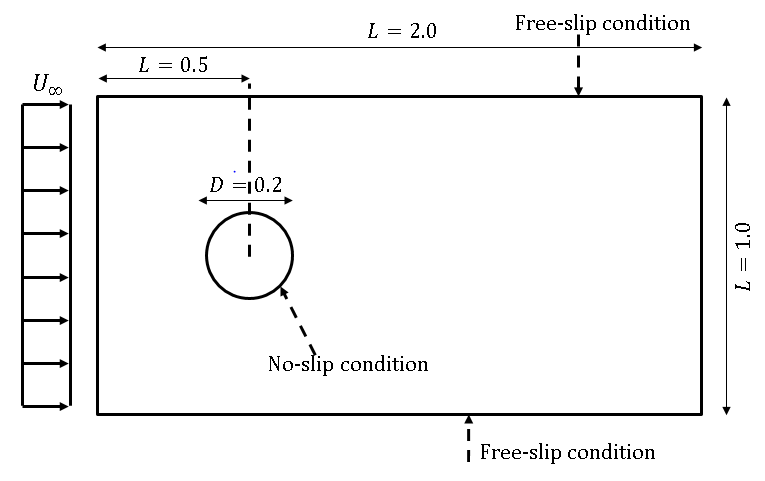
\includegraphics[height=6.0cm]{figure/cylinder/domain.png}
	\caption{Physical domain for flow over circular cylinder.}
	\label{fig:cylinderDomain}
\end{figure}
%

%
\begin{figure}[H]
	\centering
	\subfigure[Pressure contour for $Re = 100$]
	{
	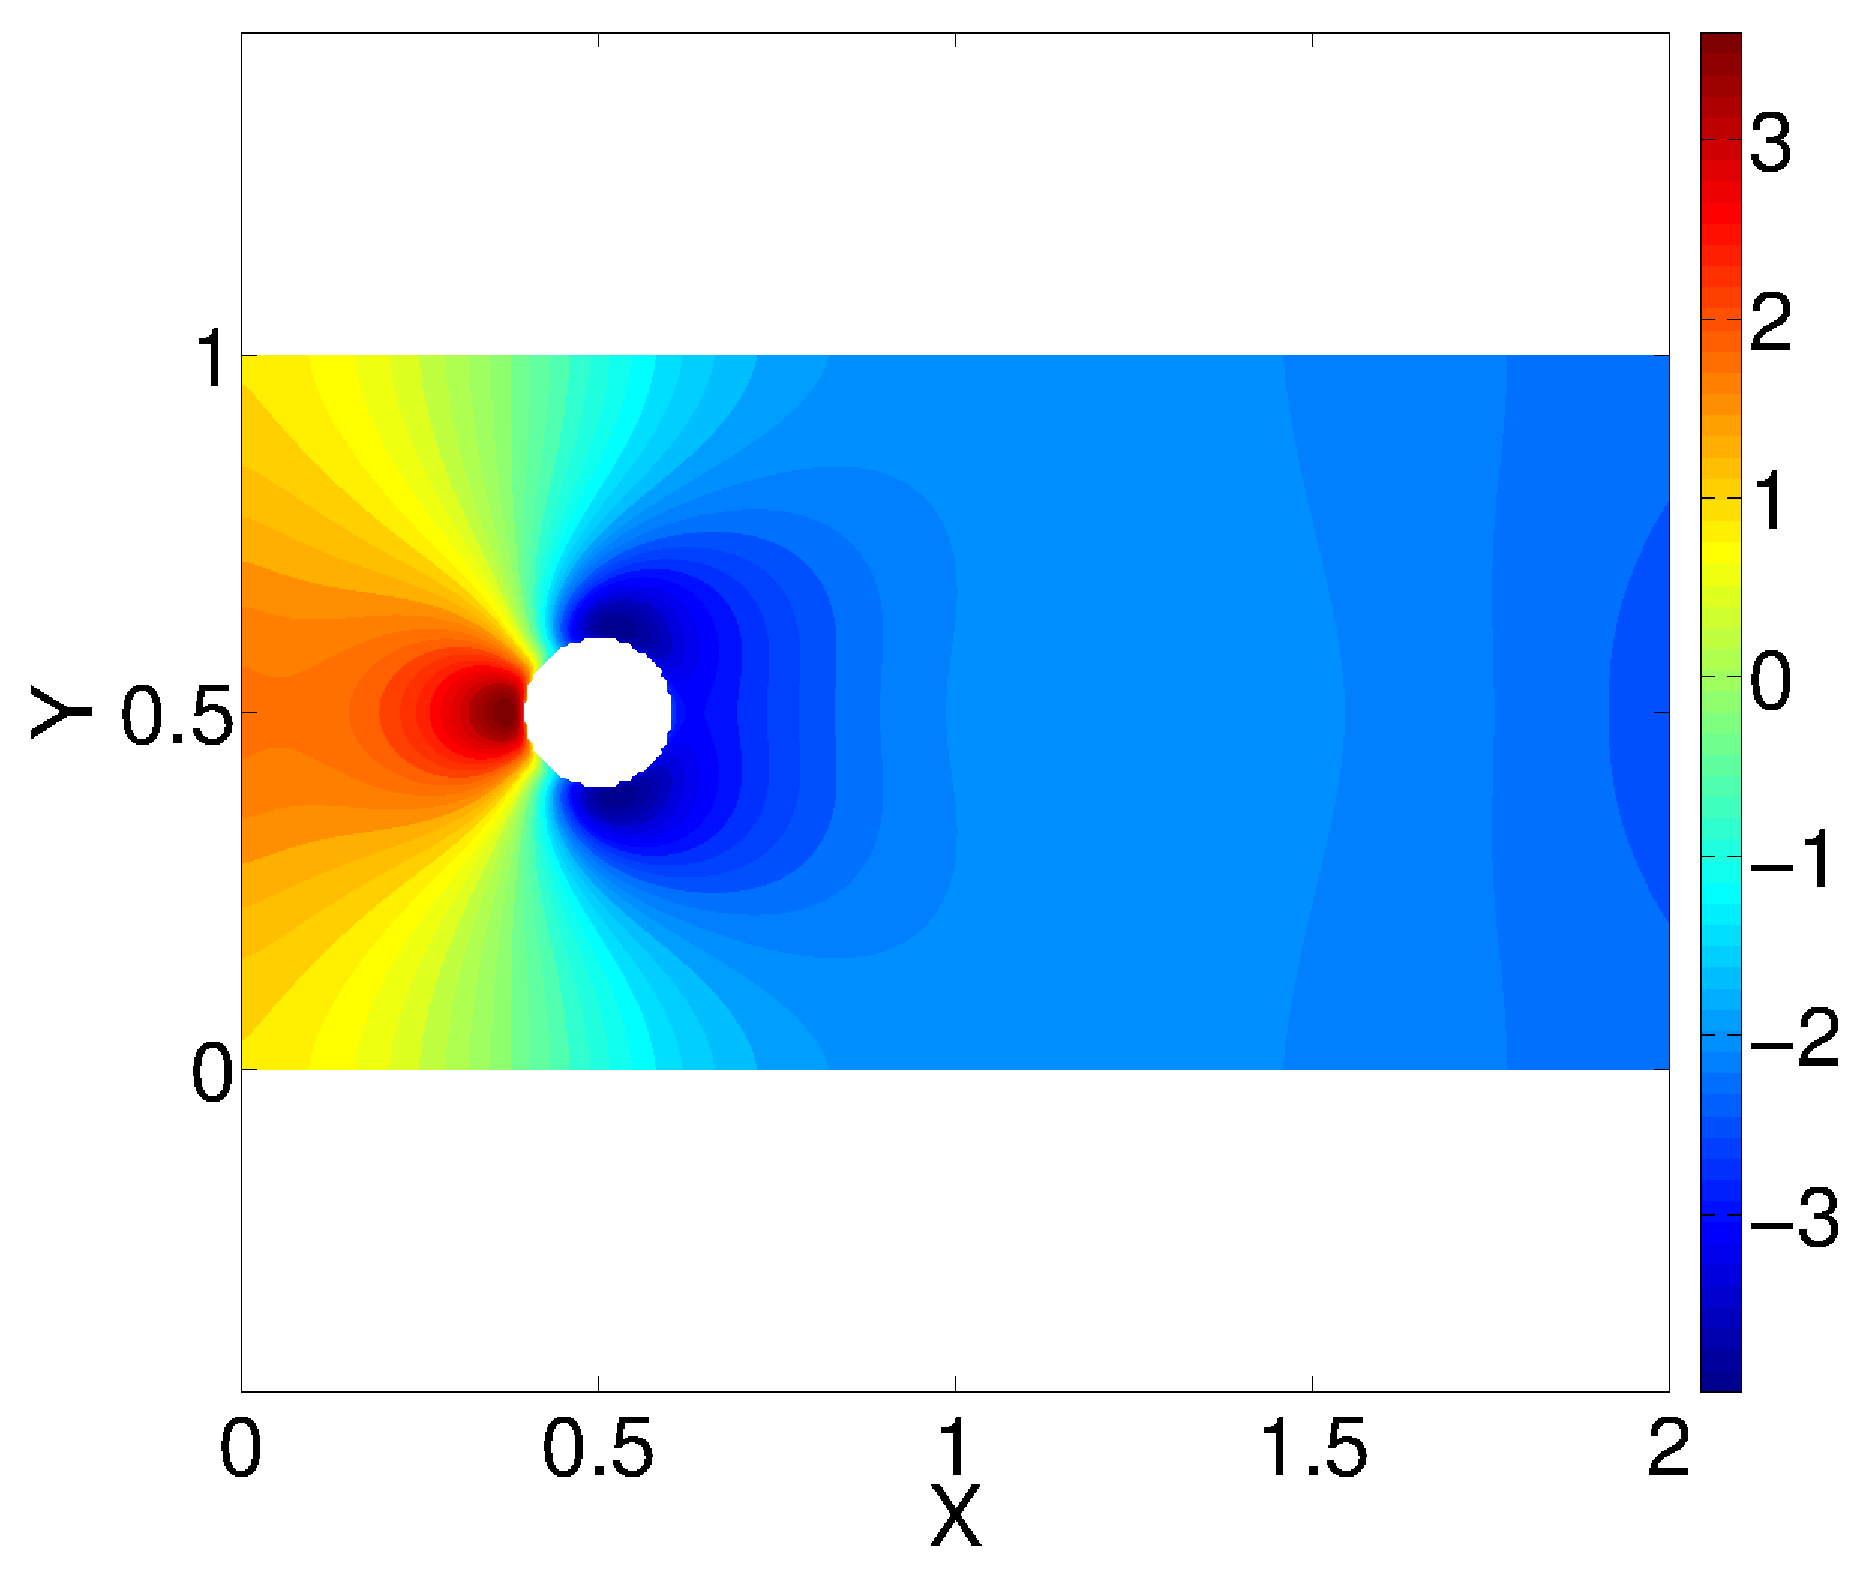
\includegraphics[height=5.0cm]{figure/cylinder/P_RE100.eps}
	}
	\quad
	\subfigure[Pressure contour for $Re = 1000$]
	{
	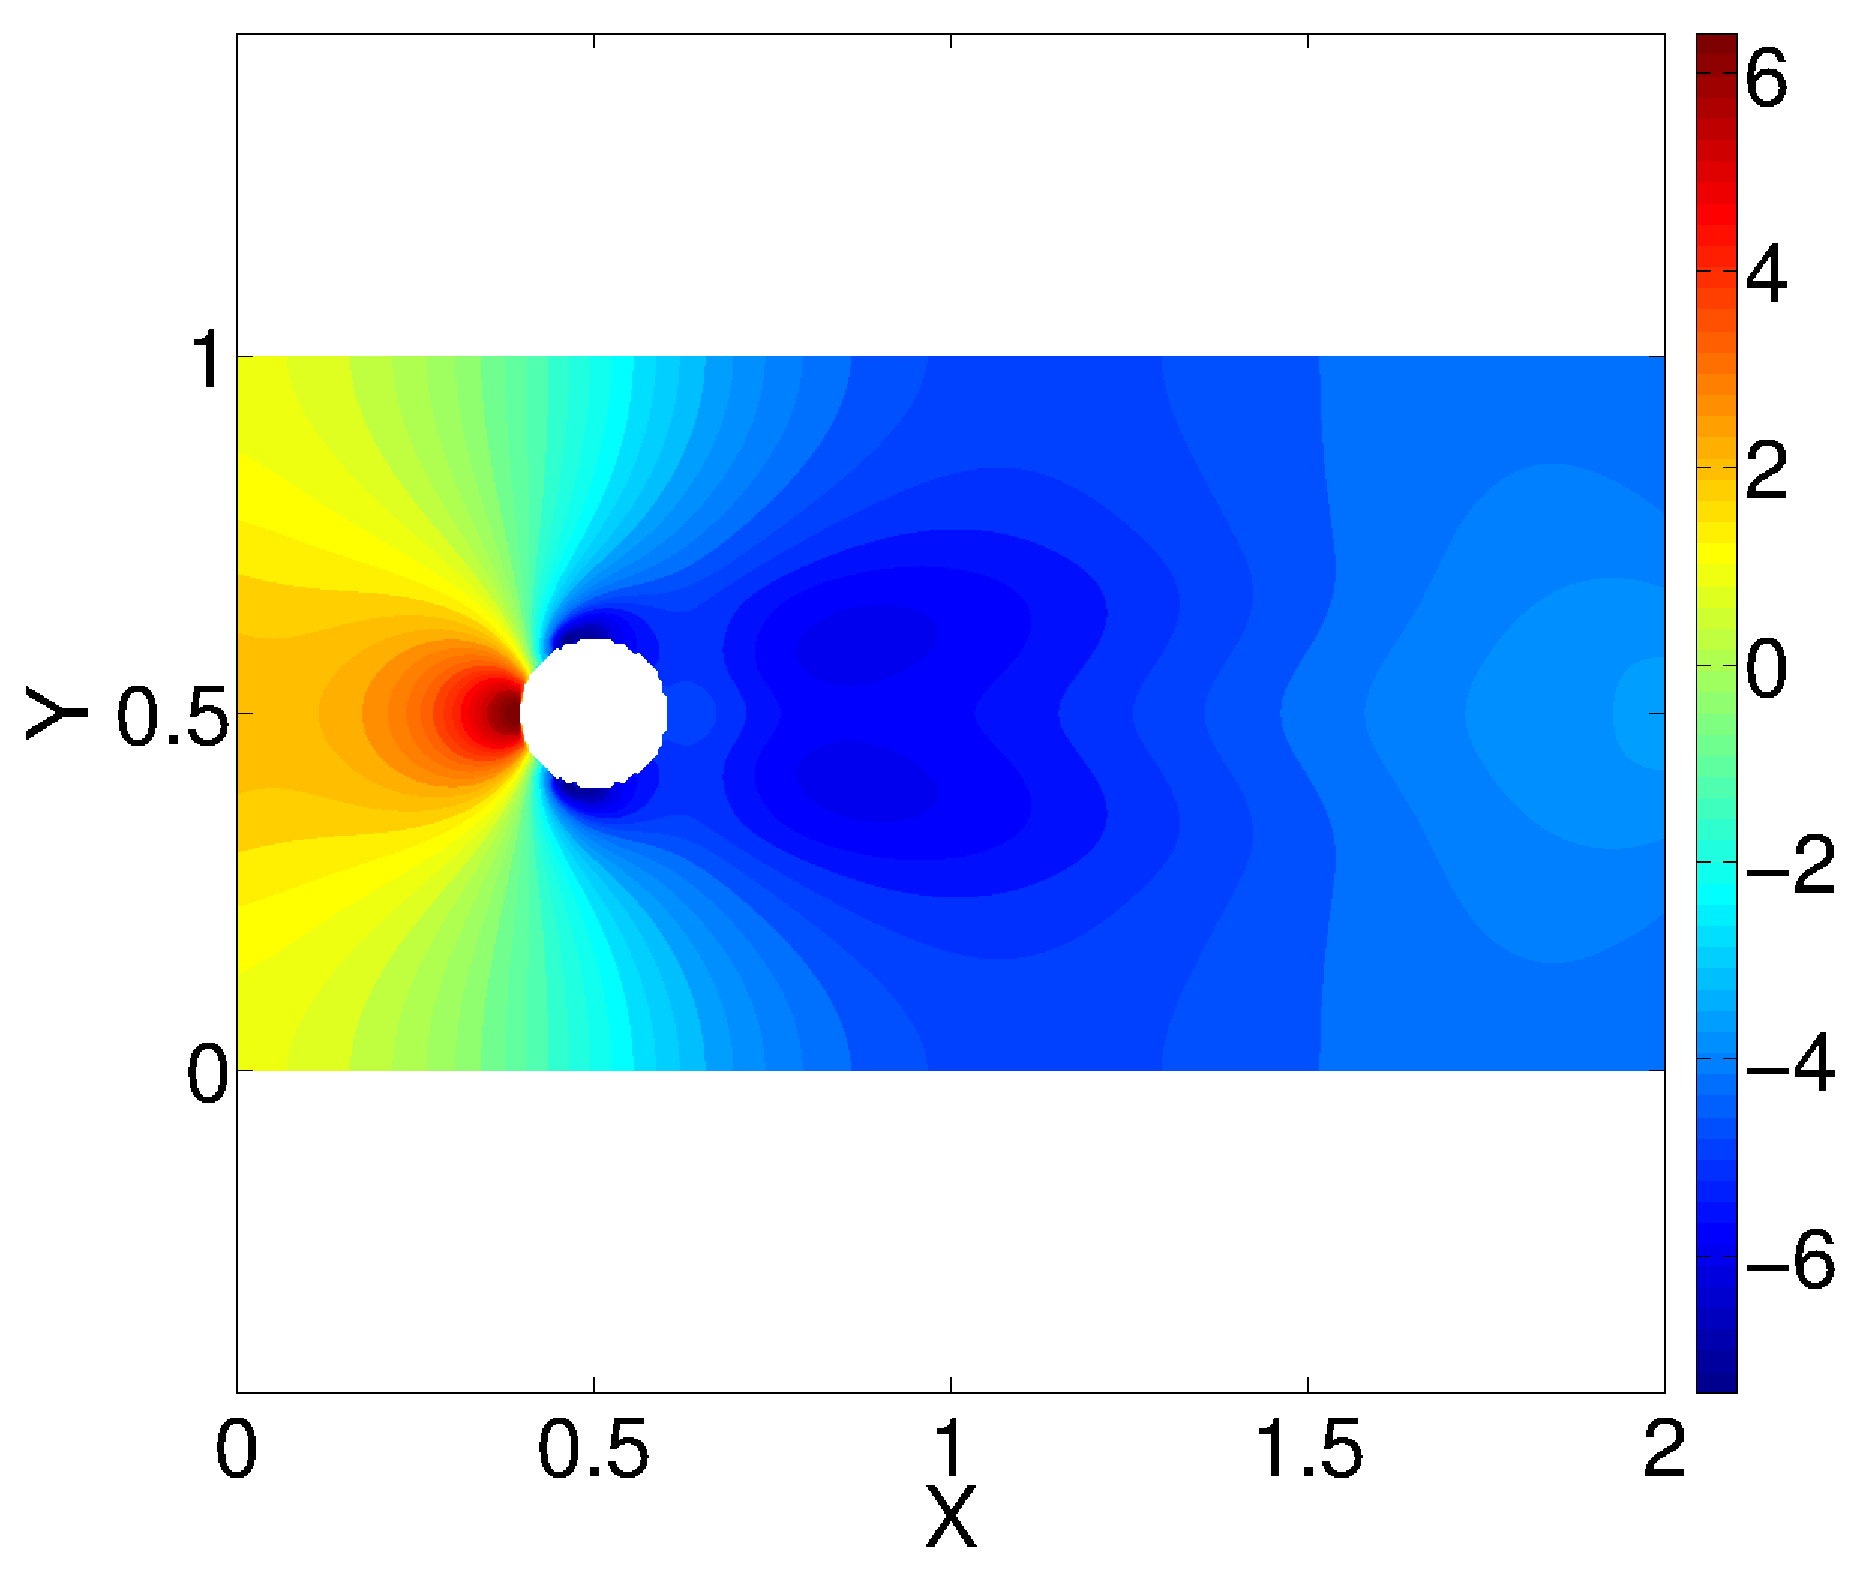
\includegraphics[height=5.0cm]{figure/cylinder/P_RE1000.eps}
	}
	\\
	\subfigure[Velocity contour for $Re = 100$]
	{
	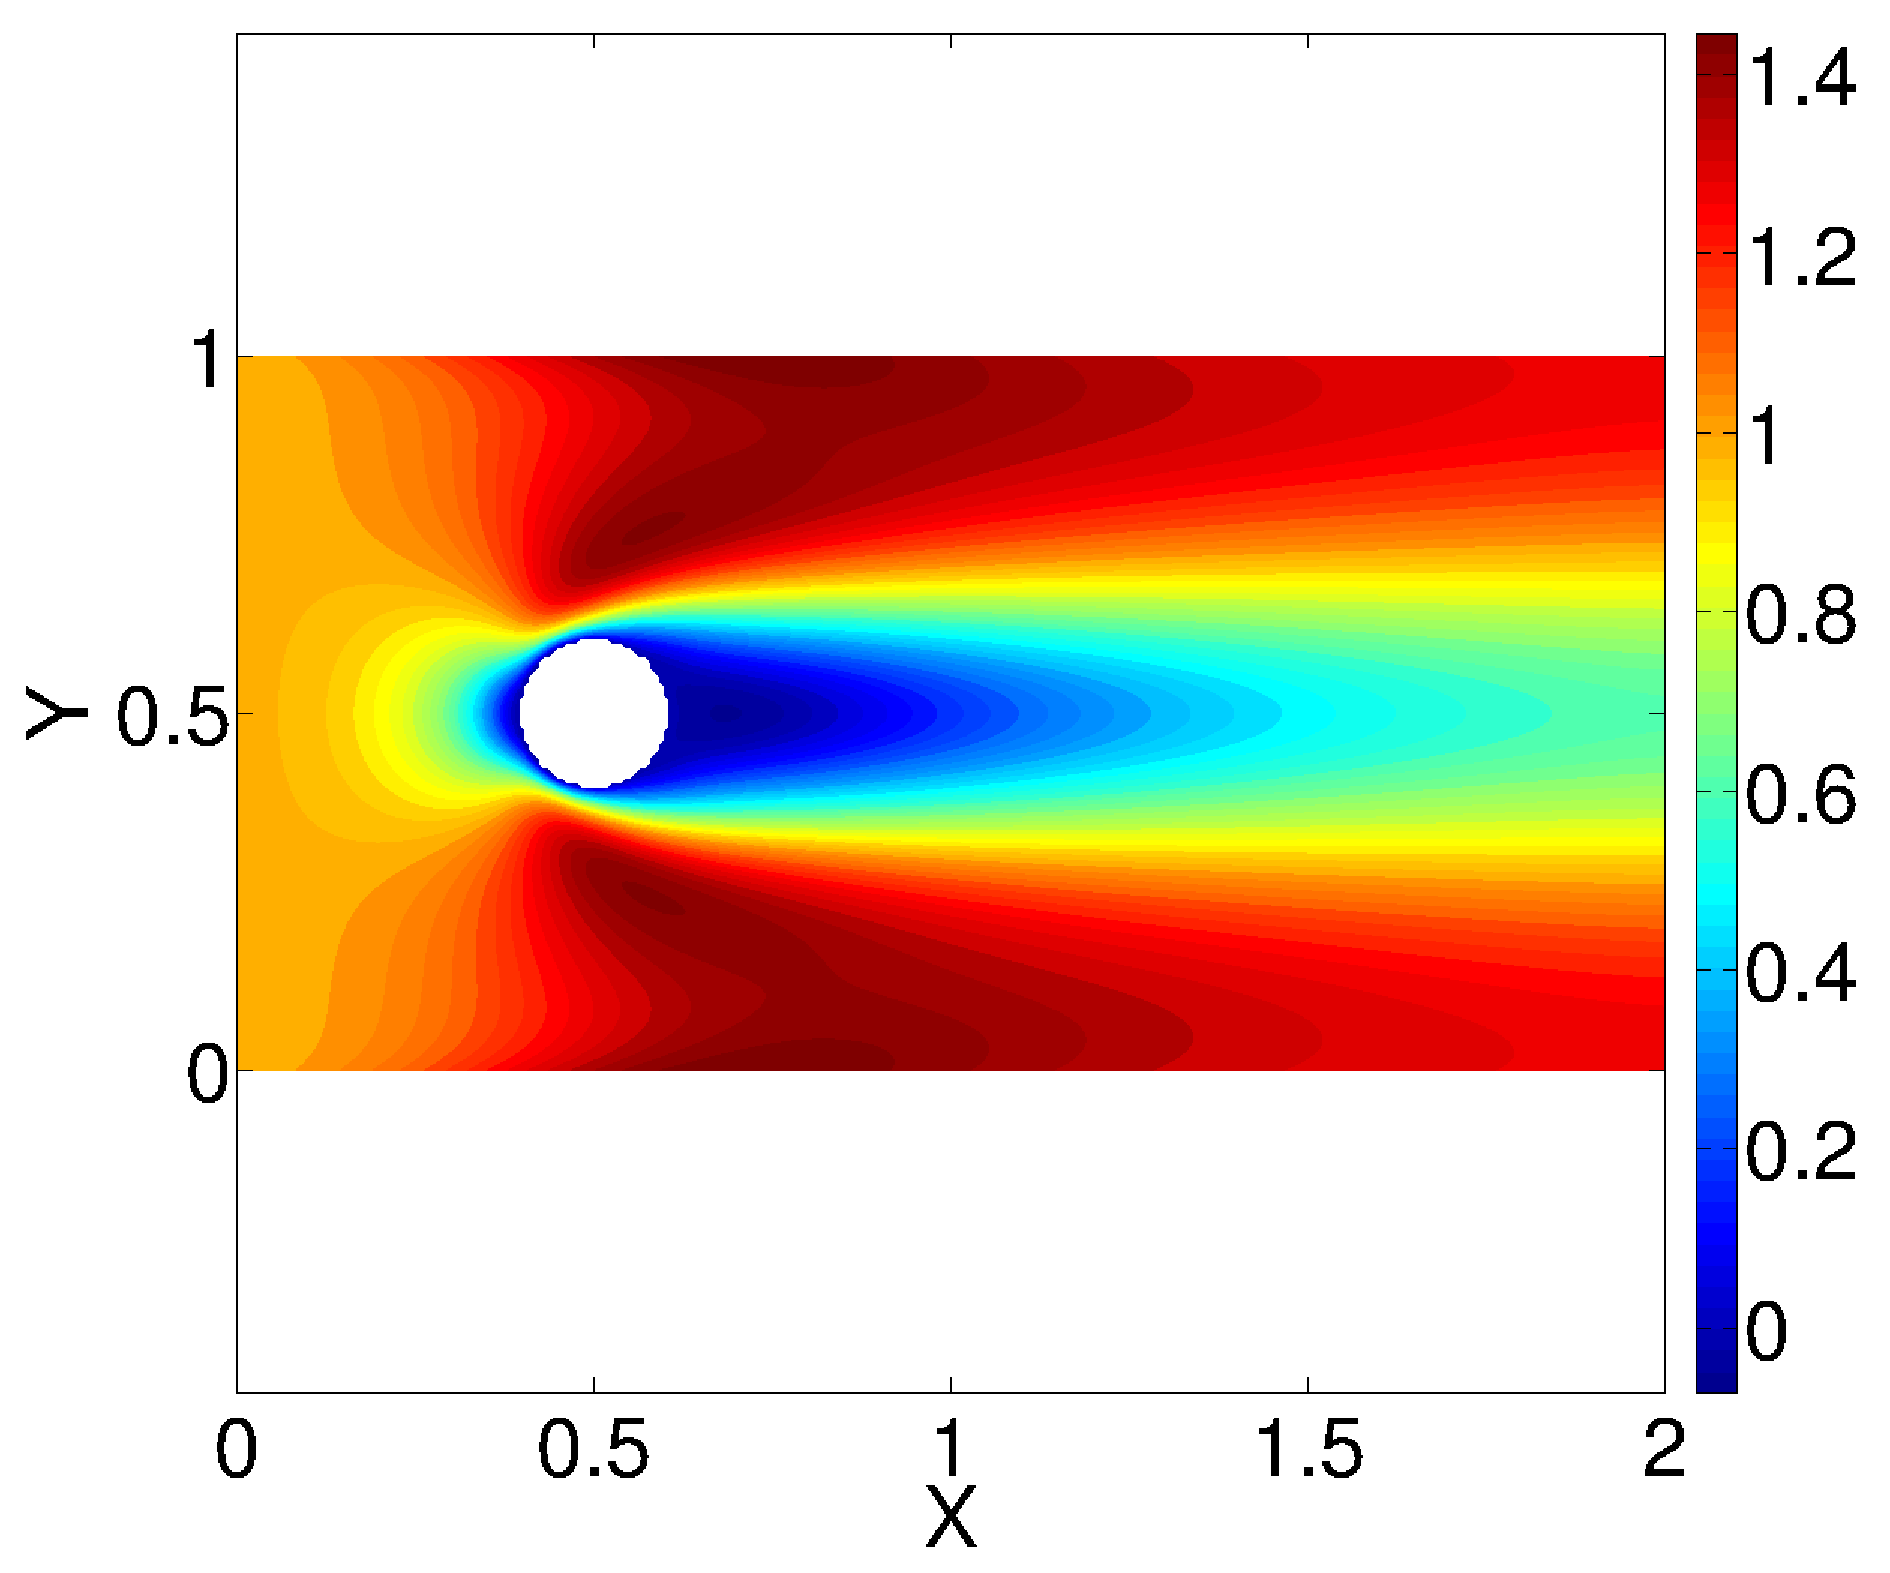
\includegraphics[height=5.0cm]{figure/cylinder/U_RE100.eps}
	}
	\quad
	\subfigure[Velocity contour for $Re = 1000$]
	{
	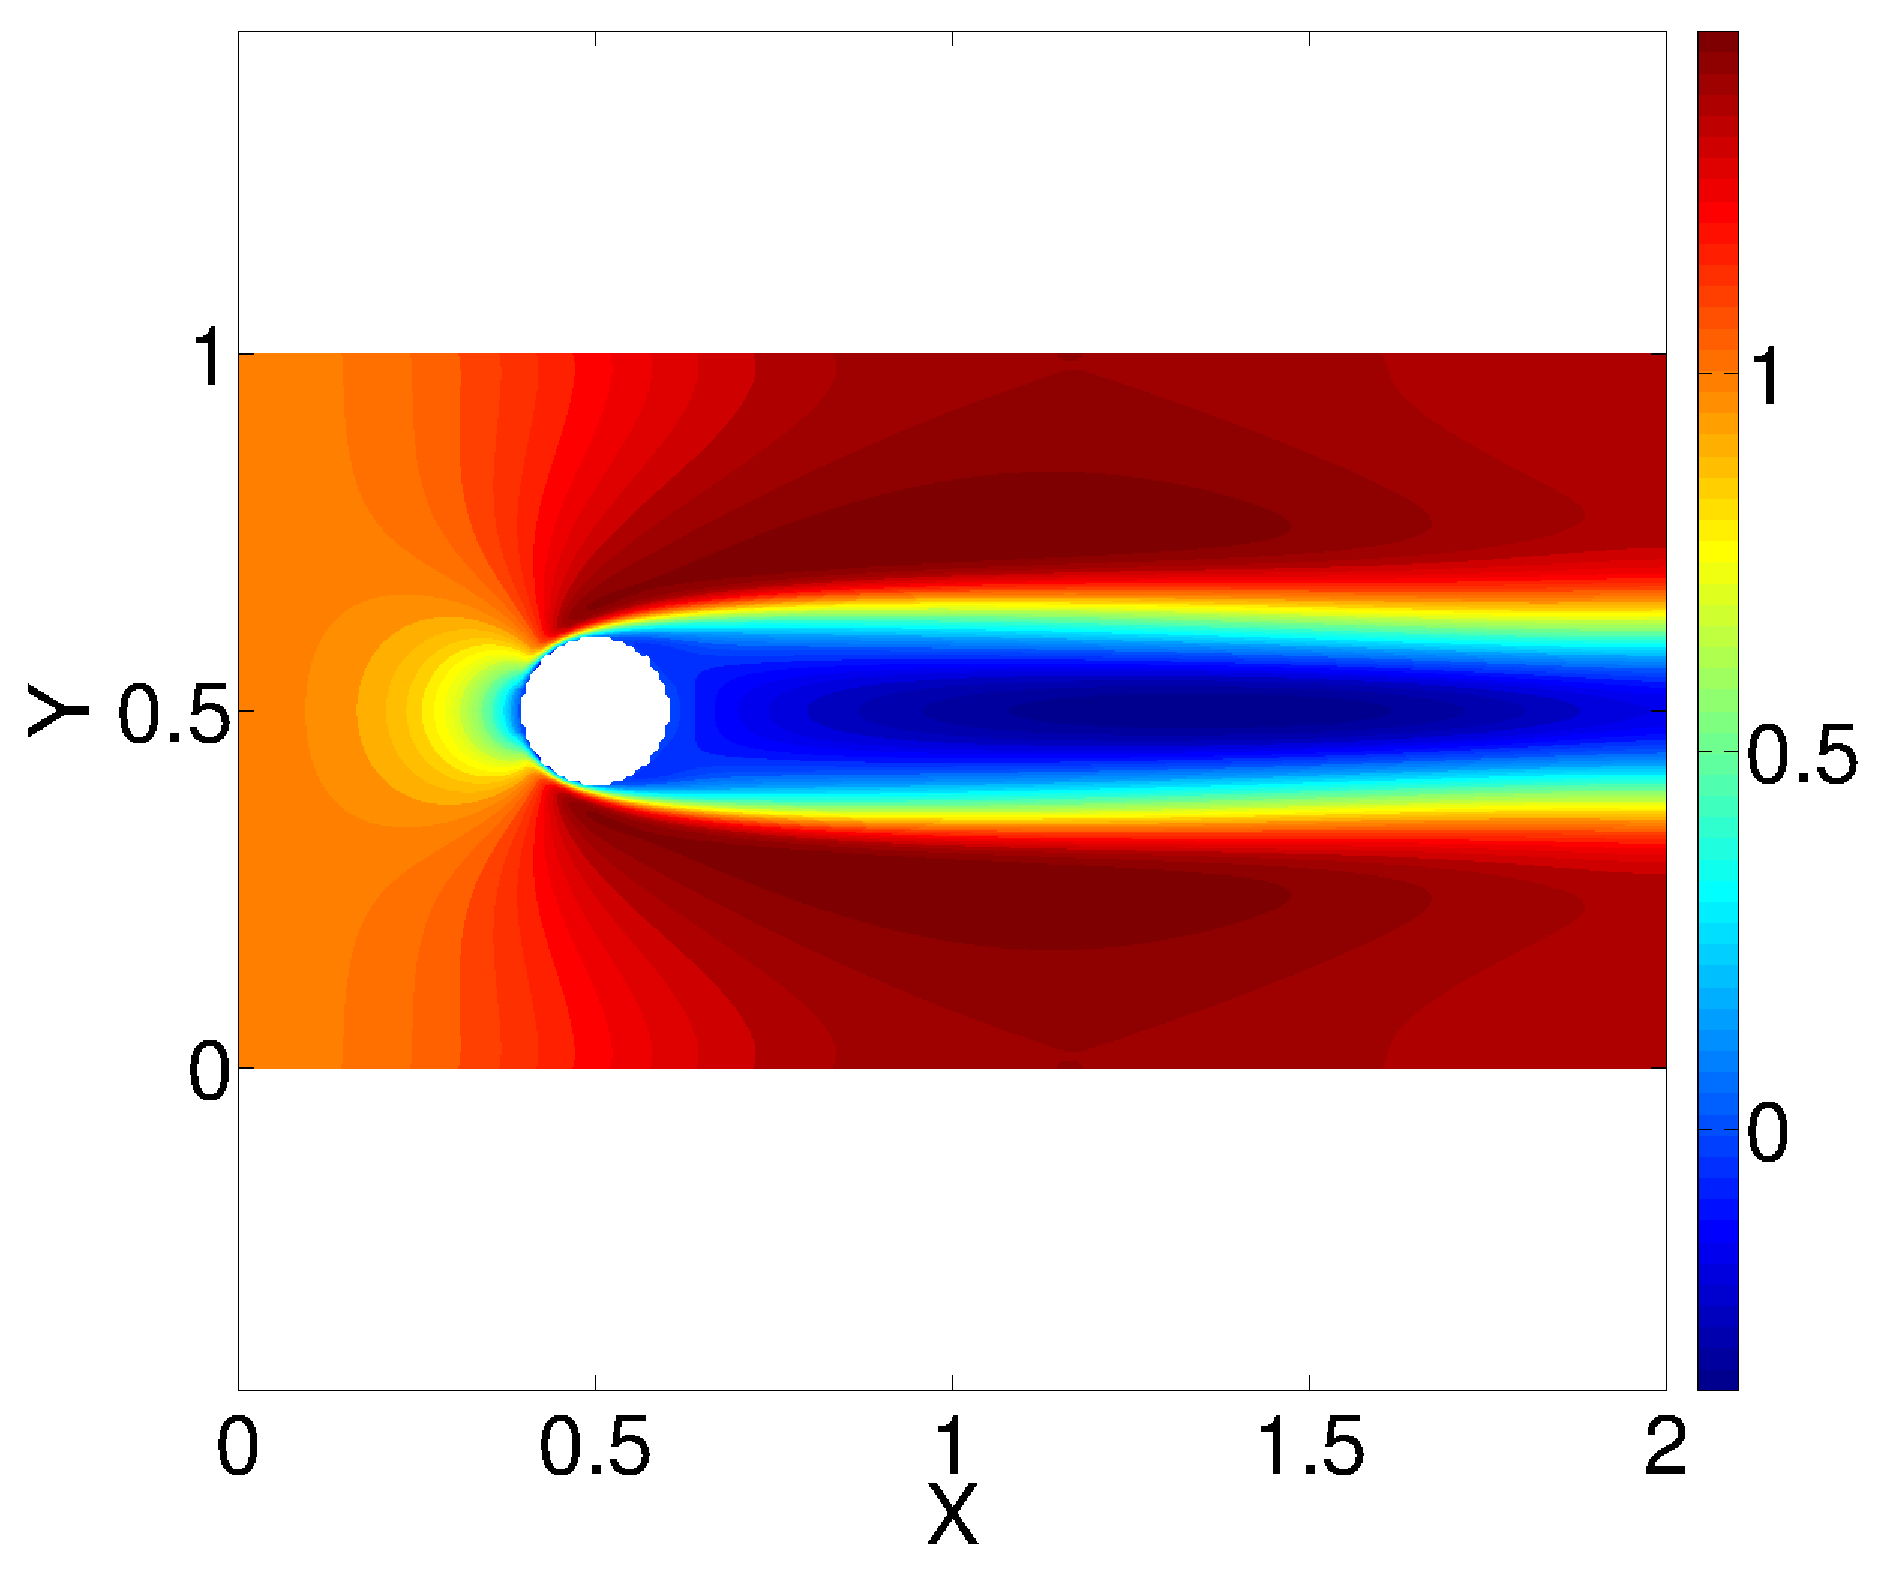
\includegraphics[height=5.0cm]{figure/cylinder/U_RE1000.eps}
	}
	\\
	\subfigure[U-velocity at $y = 0.5$ for different number of mesh nodes for $Re = 100$.]
	{
	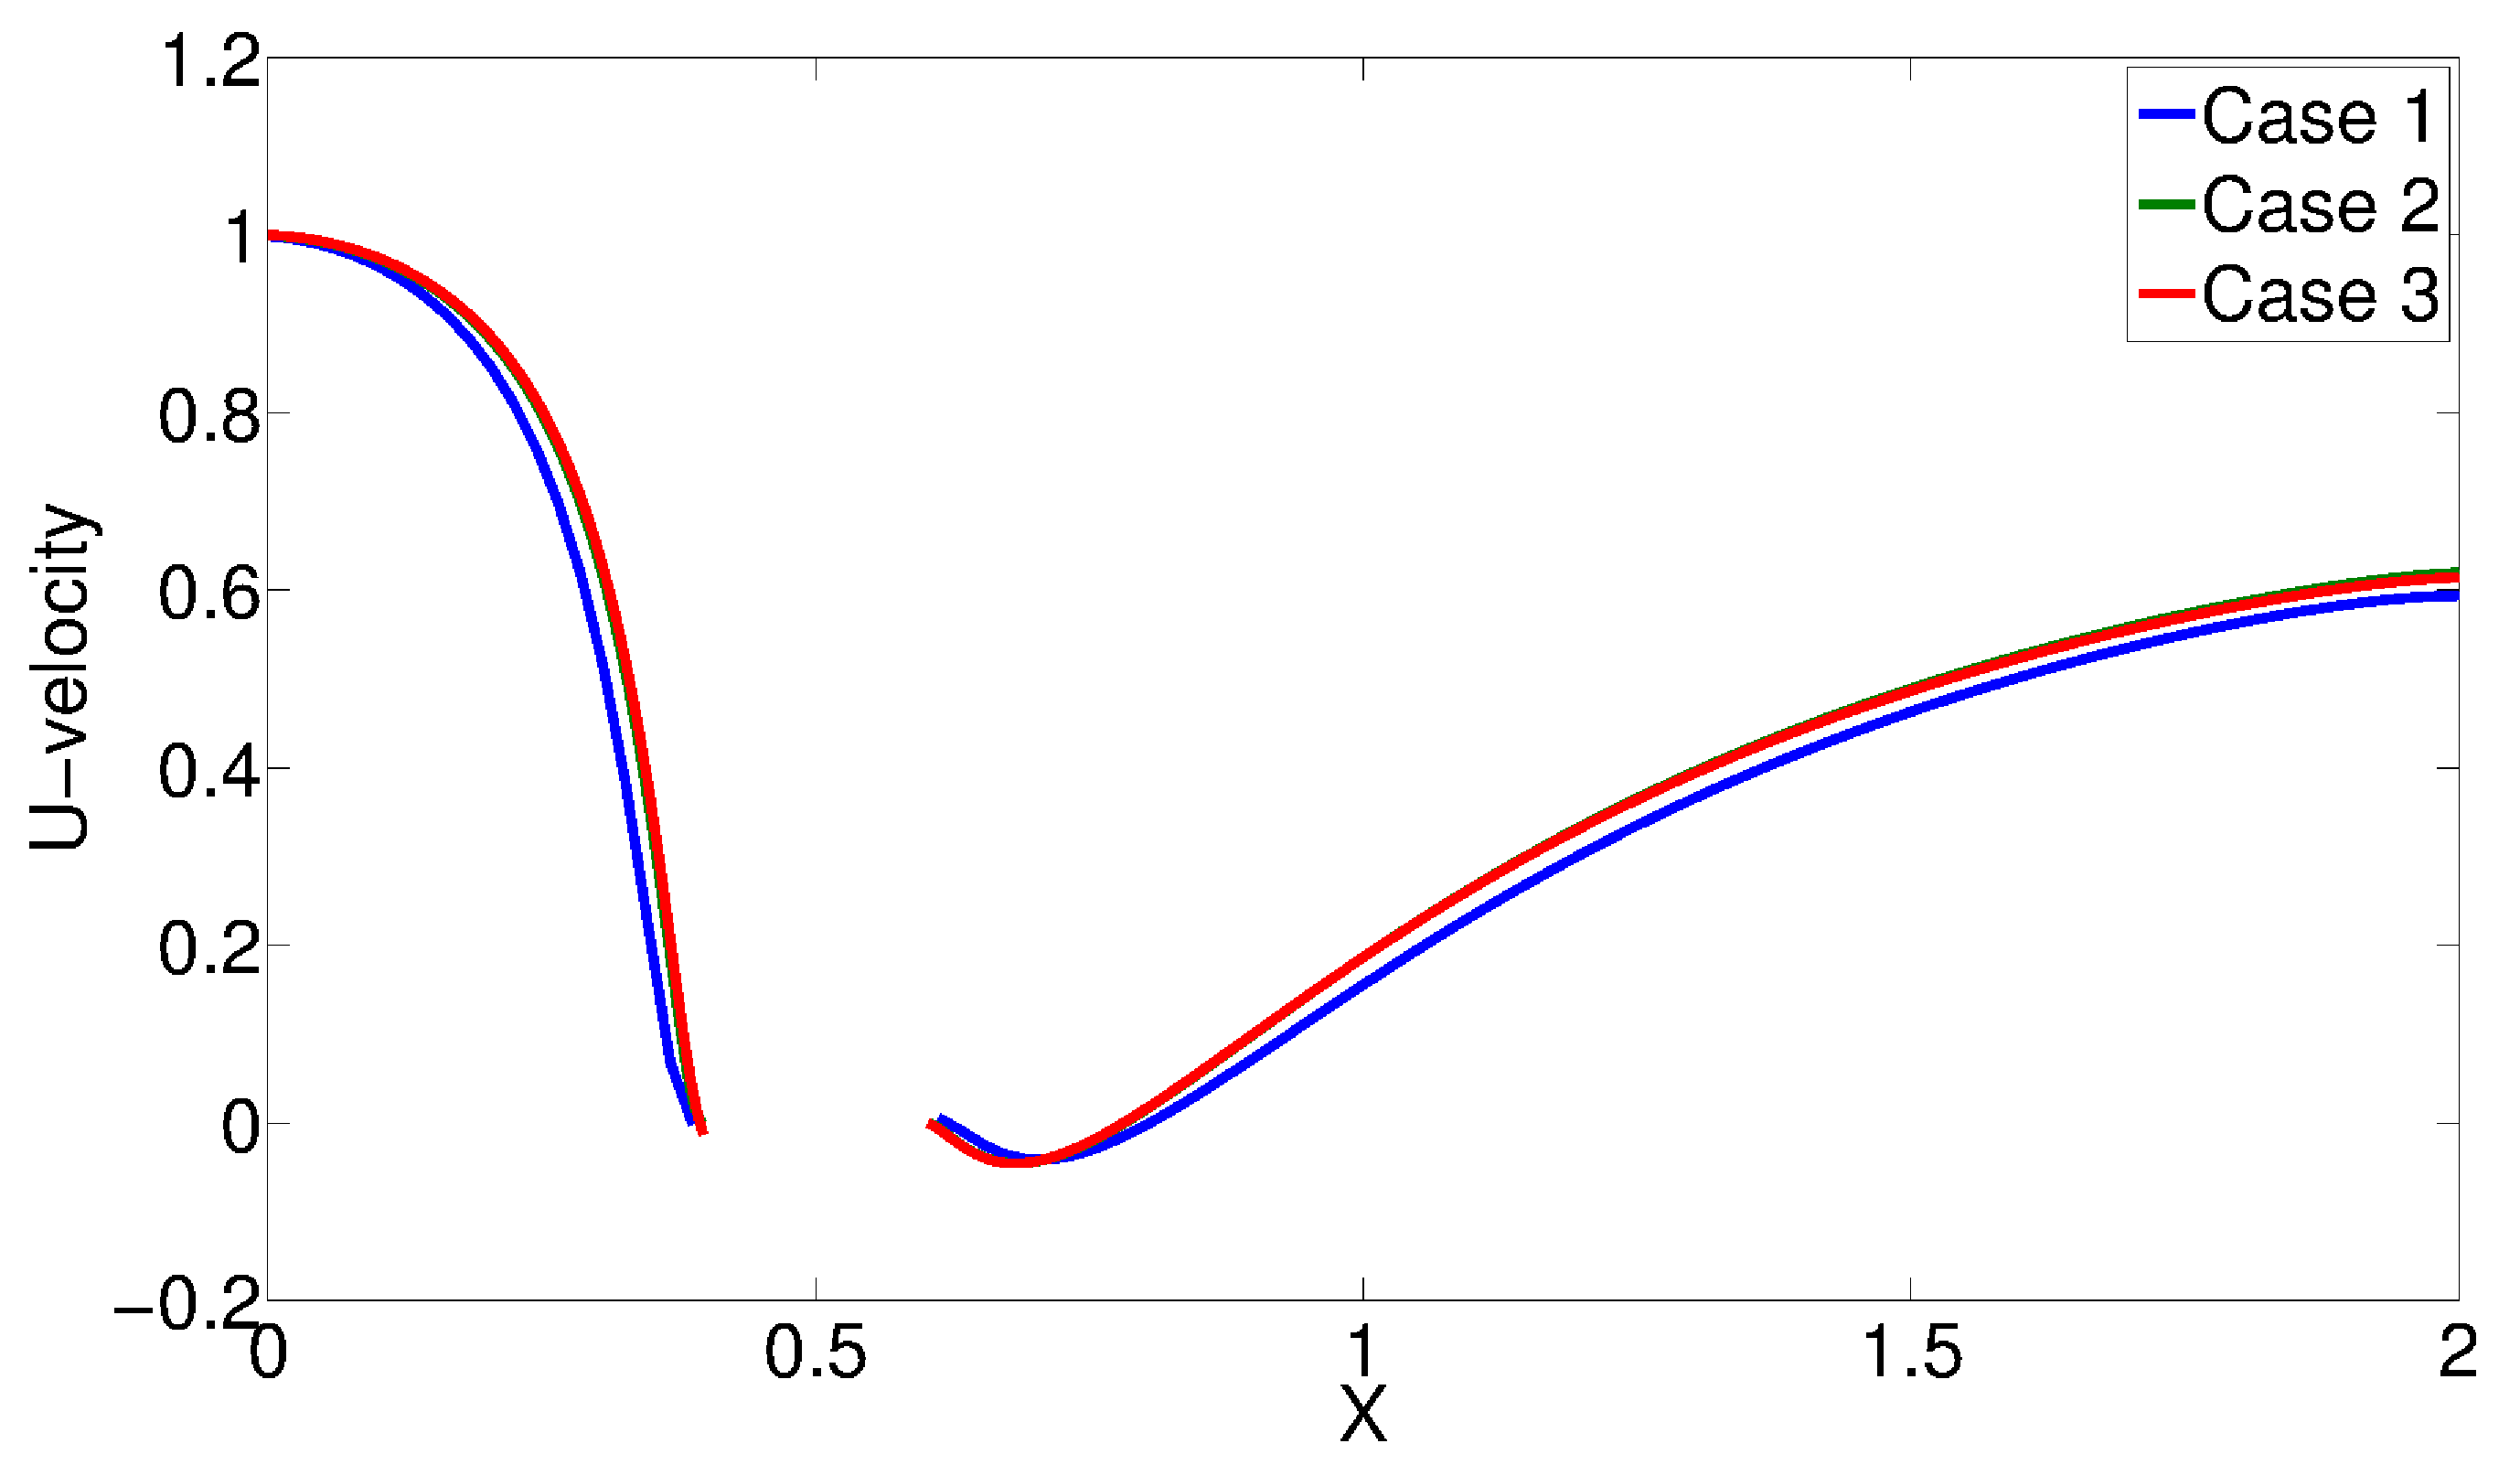
\includegraphics[height=4.0cm]{figure/cylinder/U_convergence_RE100.eps}
	}
	\quad
	\subfigure[U-velocity at $y = 0.5$ for different number of mesh nodes for $Re = 1000$]
	{
	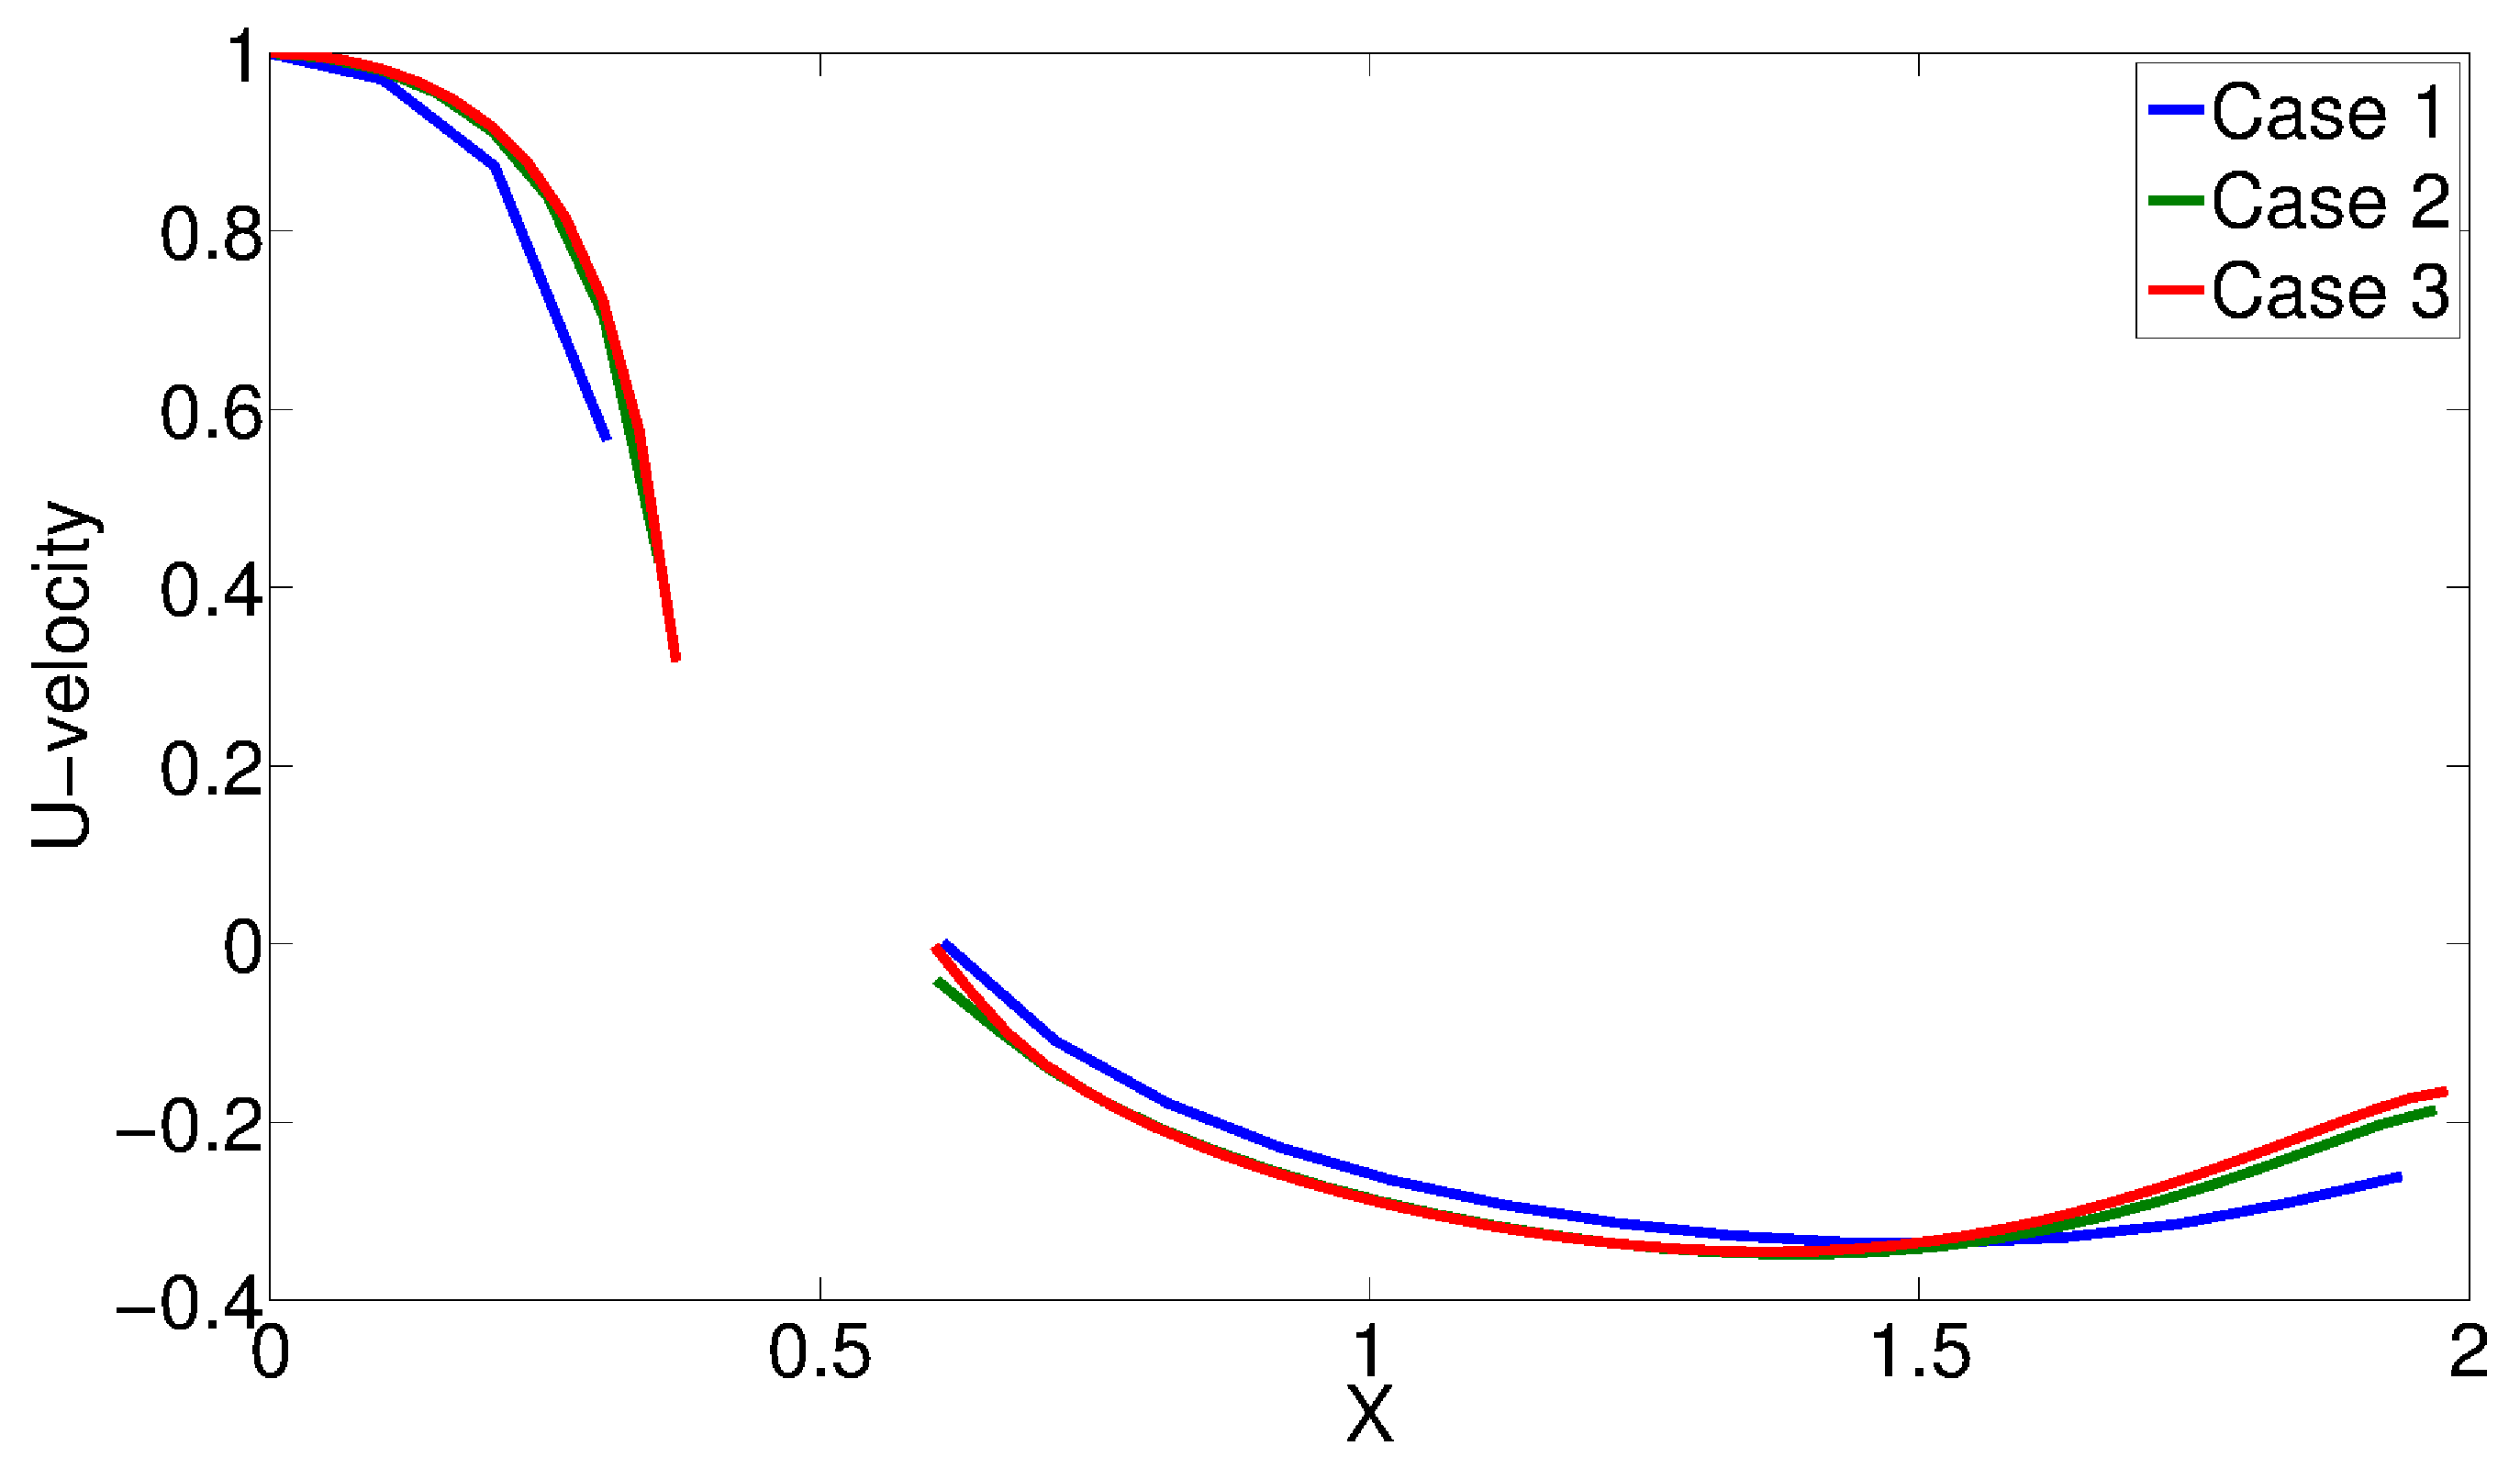
\includegraphics[height=4.0cm]{figure/cylinder/U_convergence_RE1000.eps}
	}
	\\
	\subfigure[V-velocity at $x = 0.25$ for different number of mesh nodes for $Re = 100$]
	{
	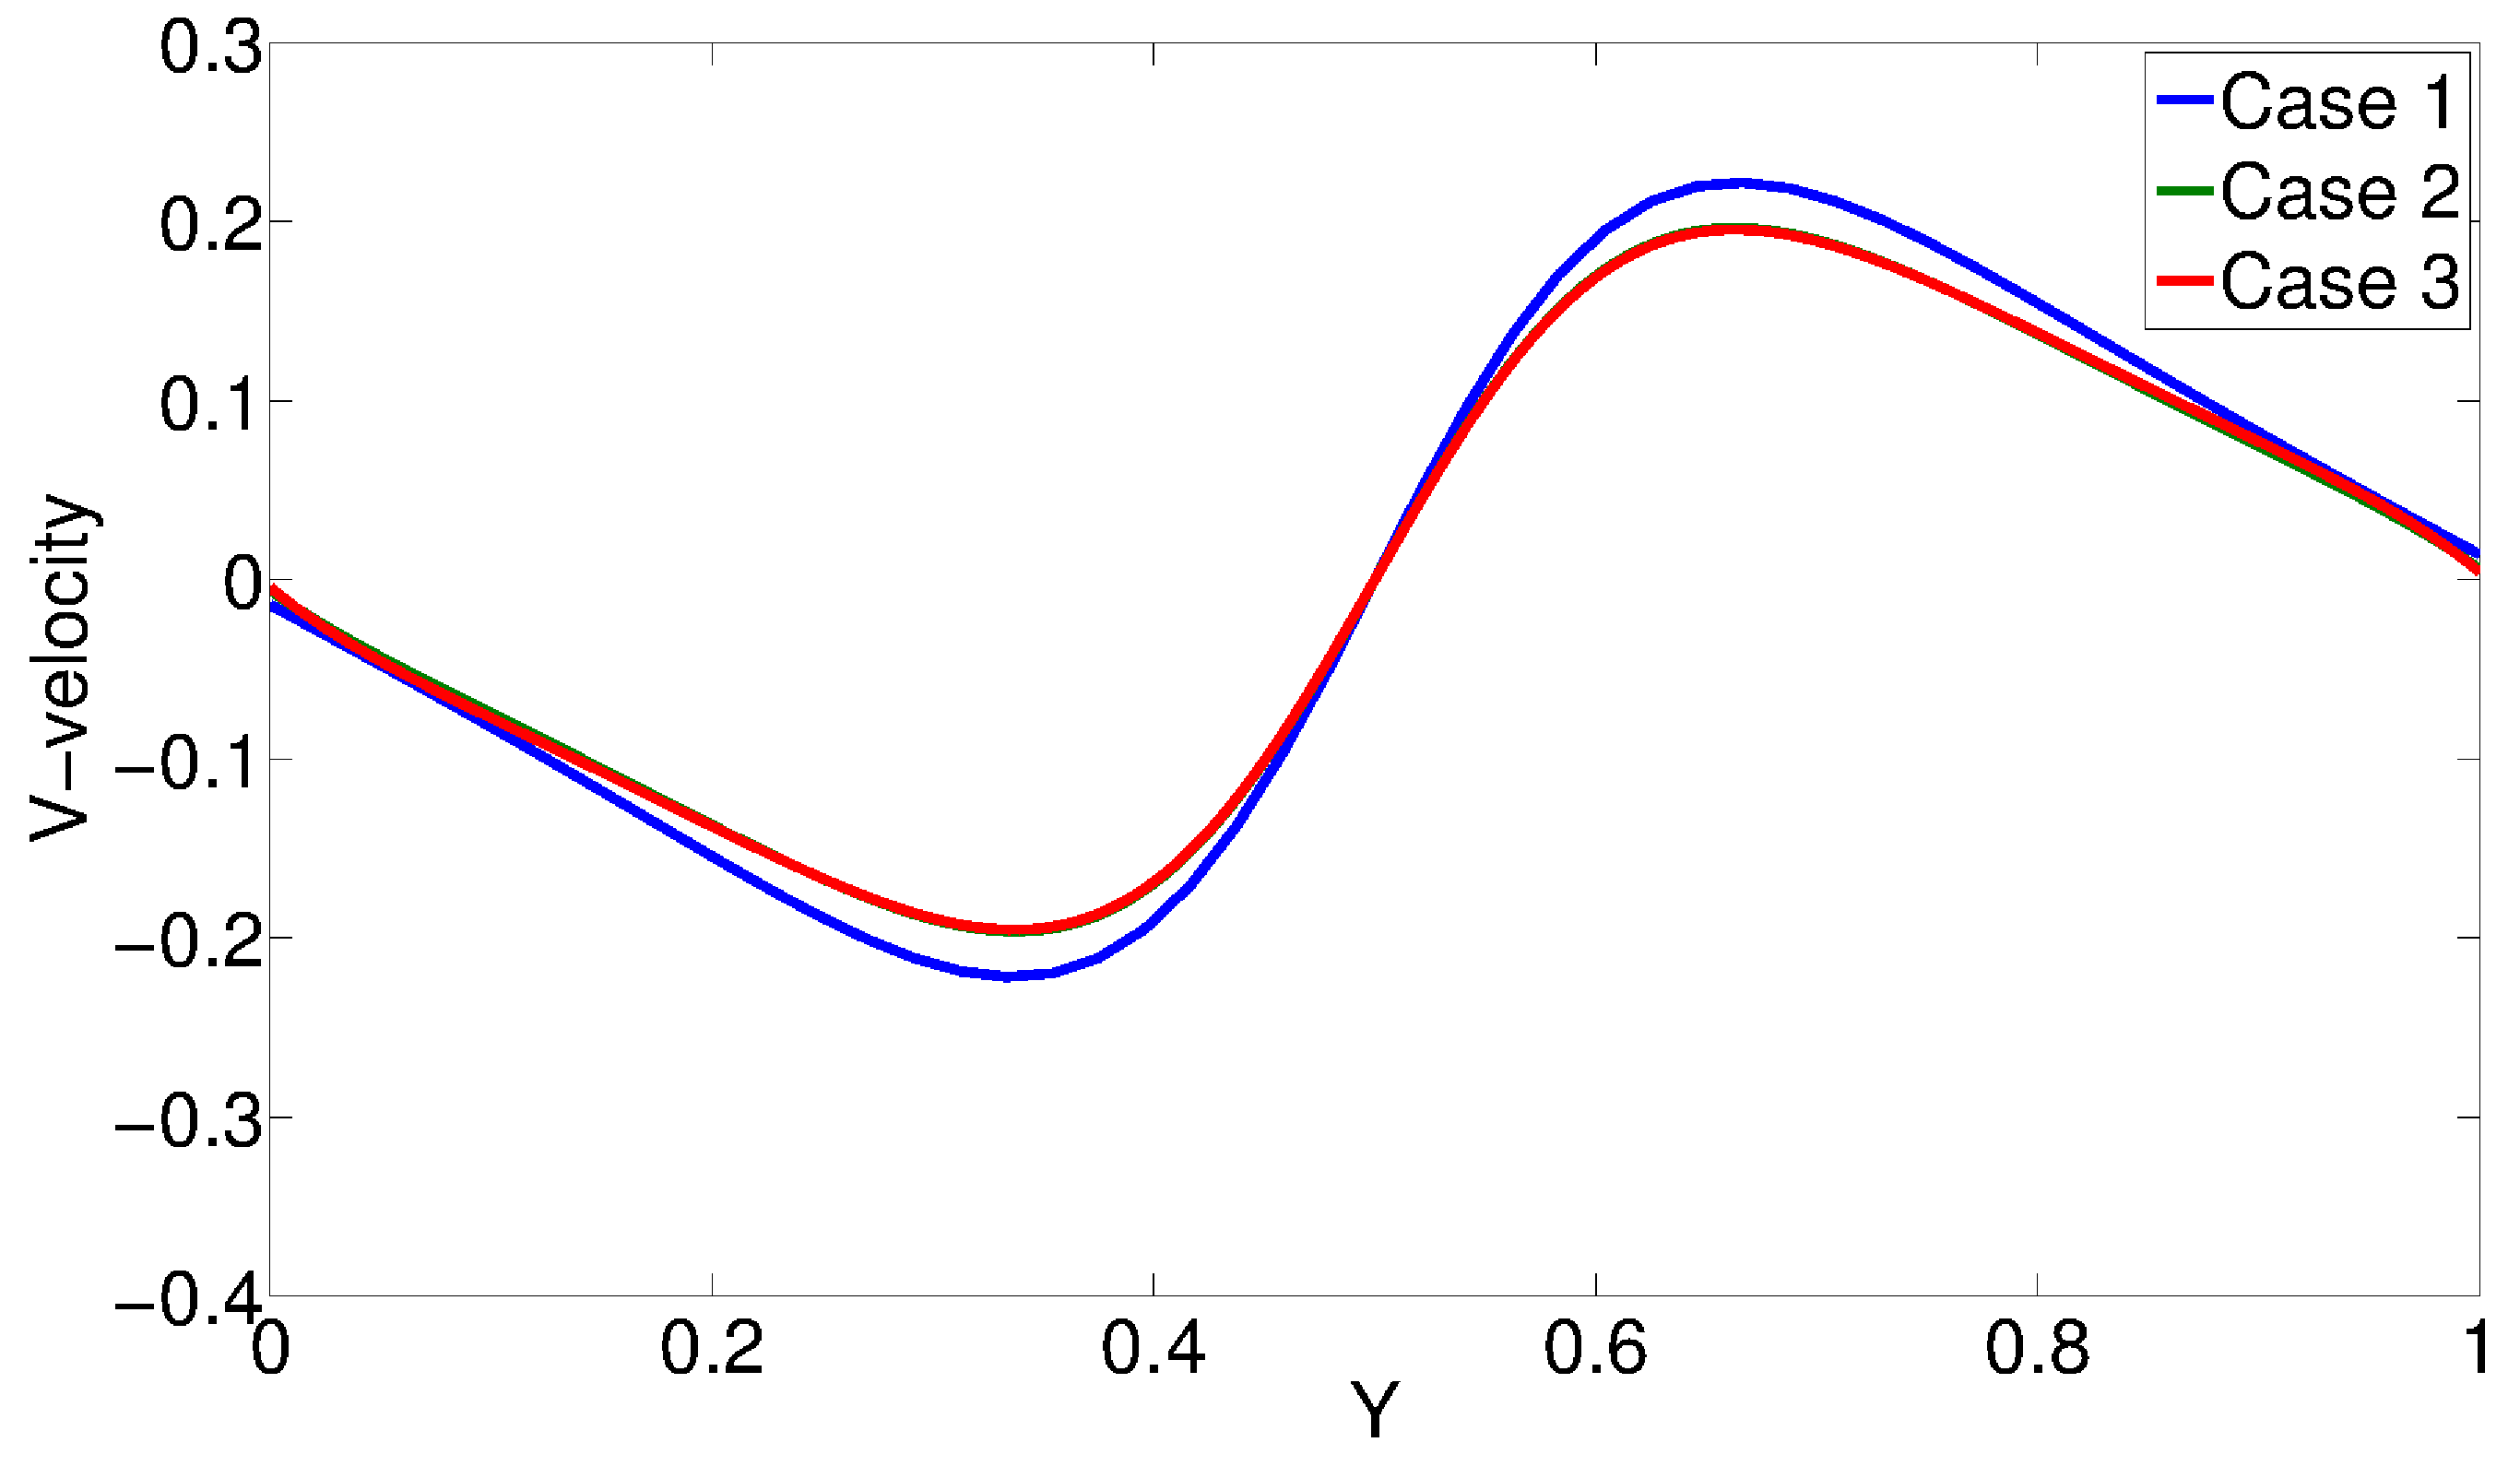
\includegraphics[height=4.0cm]{figure/cylinder/V_convergence_RE100.eps}
	}
	\quad
	\subfigure[V-velocity at $x = 0.25$ for different number of mesh nodes for $Re = 1000$]
	{
	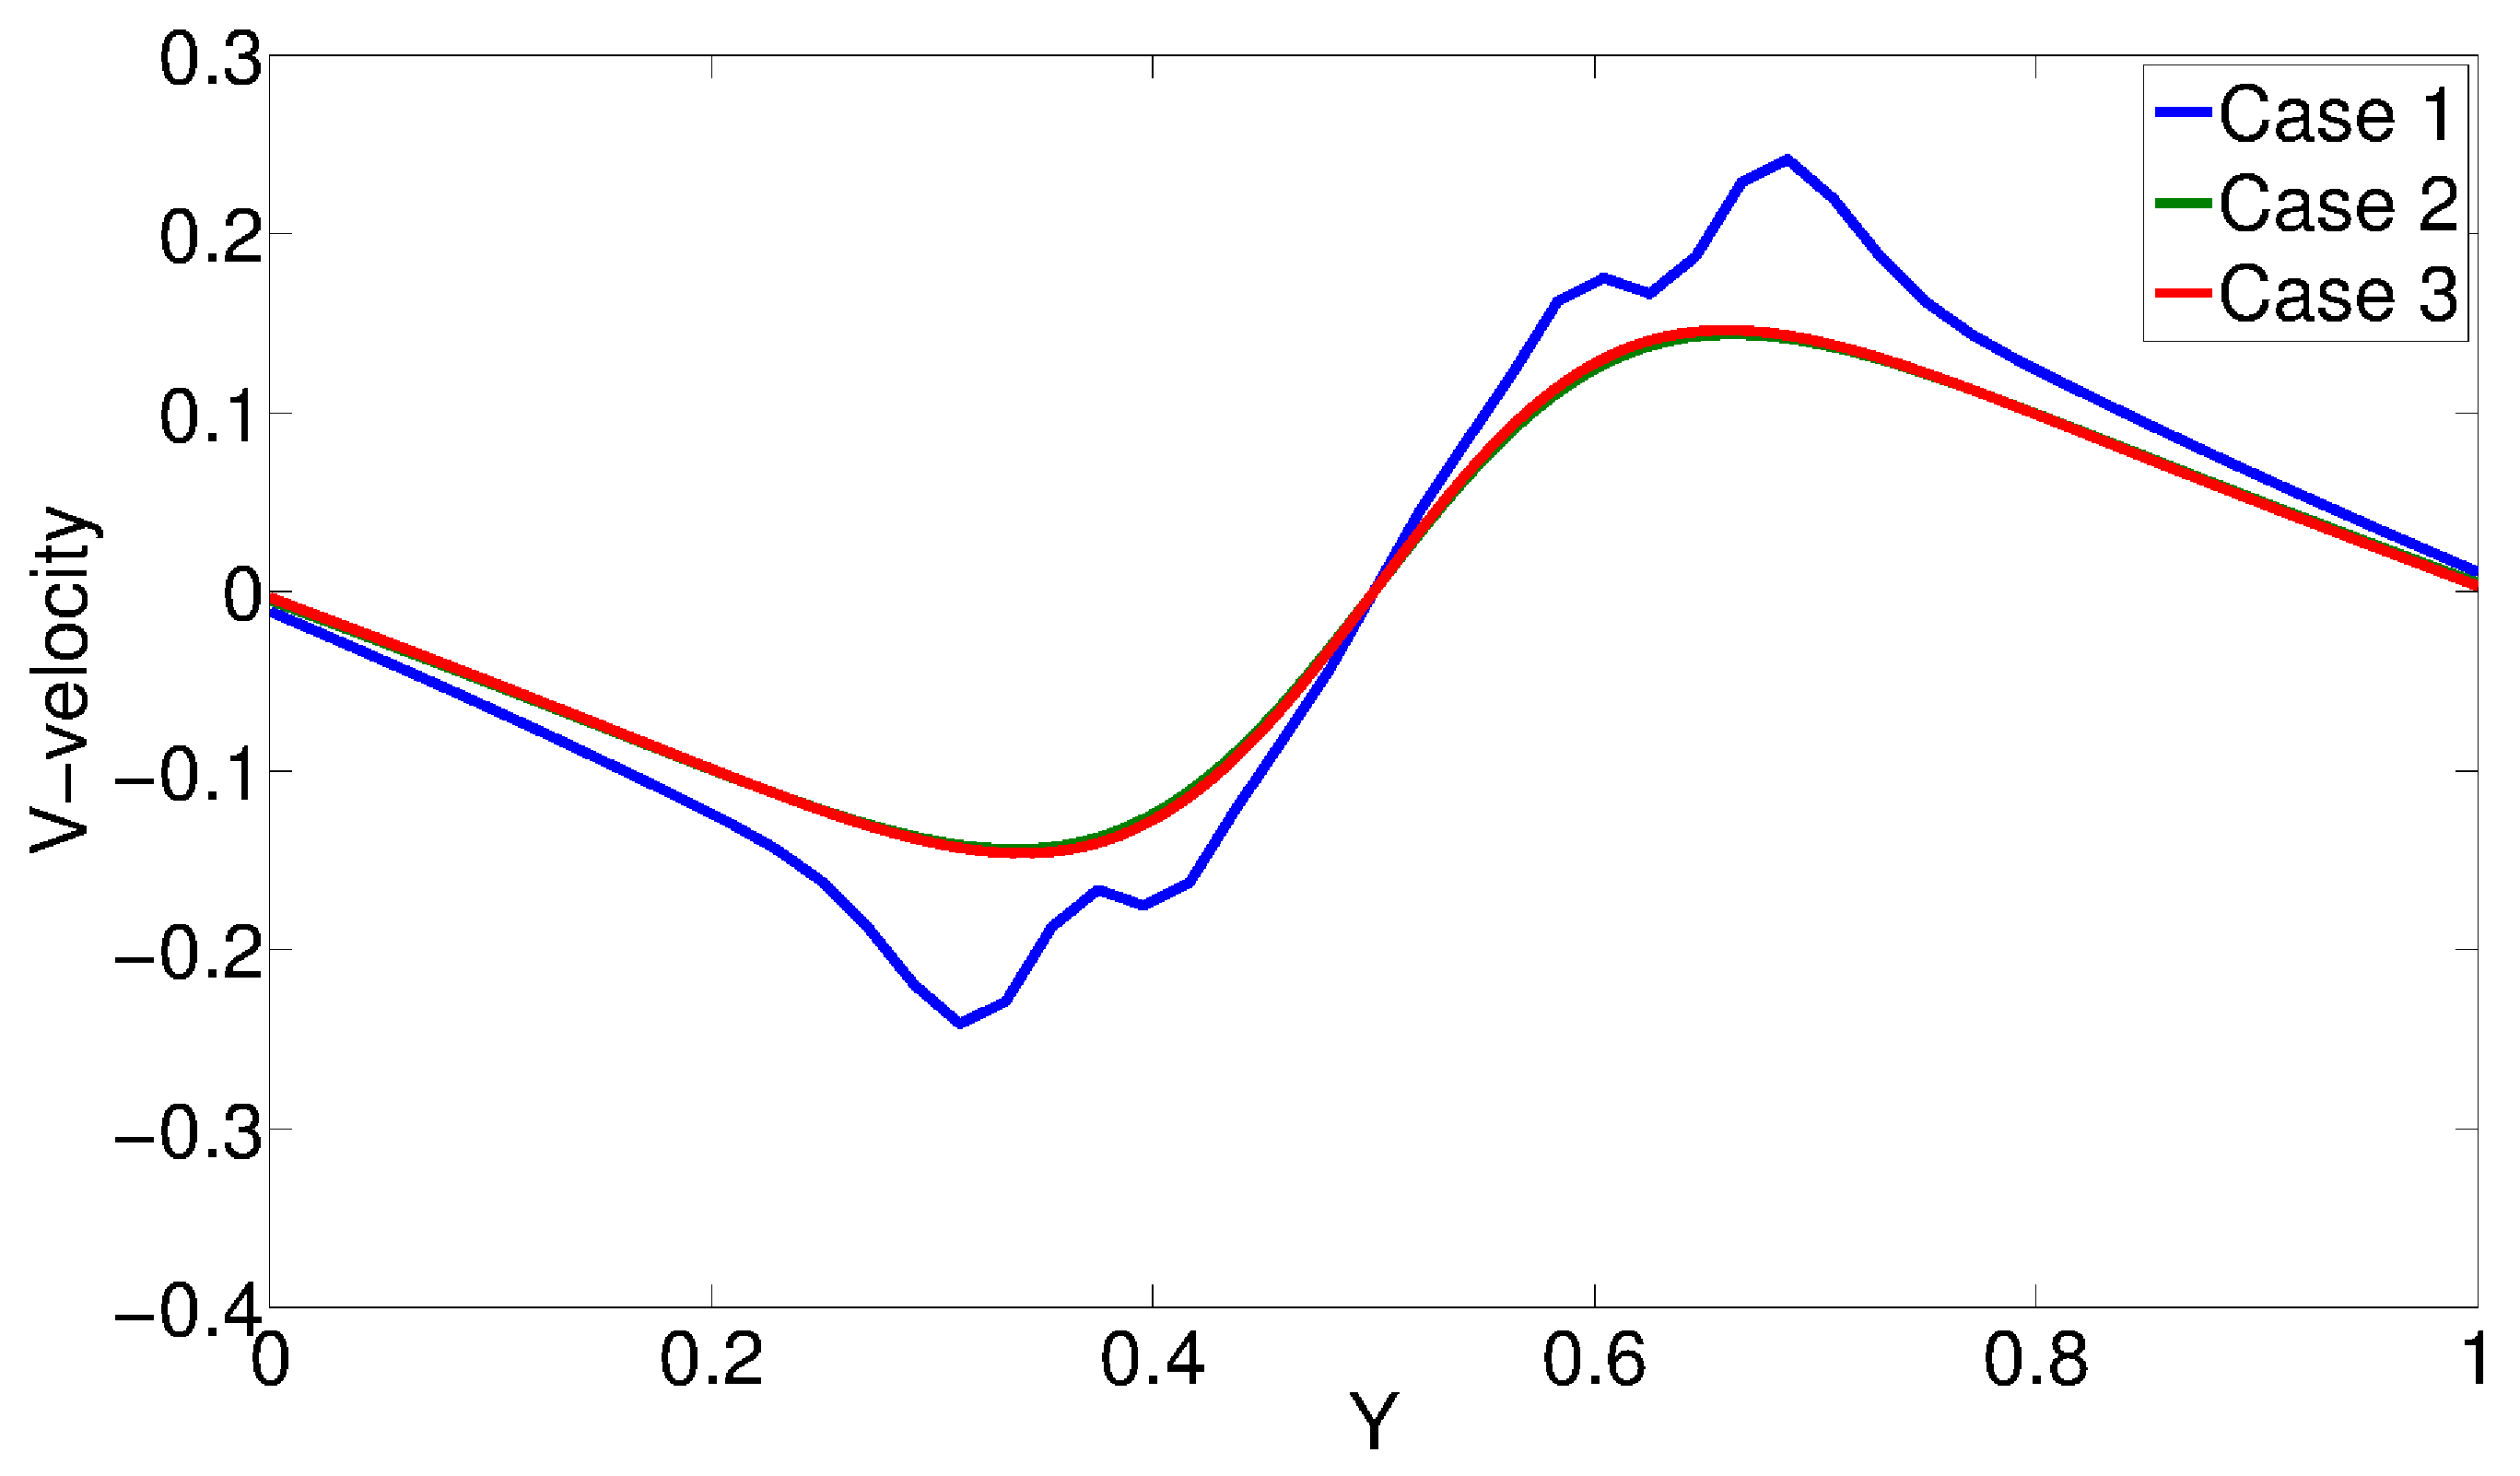
\includegraphics[height=4.0cm]{figure/cylinder/V_convergence_RE1000.eps}
	}
	\caption{Results of convergence study for flow over cylinder. Case 1, 2, and 3 are domains with $100 \times 50$, $200 \times 100$, $300 \times 150$ nodes.}
	\label{fig:convegence_study}
\end{figure}
%

The time history of force terms on the cylinder surface are shown in Figure \ref{fig:cylinderForceTerms}. We choose five probe locations on the surface to track the force values. It should be noted that these are the force terms added to the Navier-Stokes equations to represent the boundary, not the forces acting on the surface of the cylinder due to hydrodynamic pressure. As shown in Figure \ref{fig:cylinderForceTerms}, the values of the forcing function starts oscillating at the beginning and reaches a steady-state value.

%
\begin{figure}[H]
	\centering
	\subfigure[Forcing term in $x$ direction.]
	{
	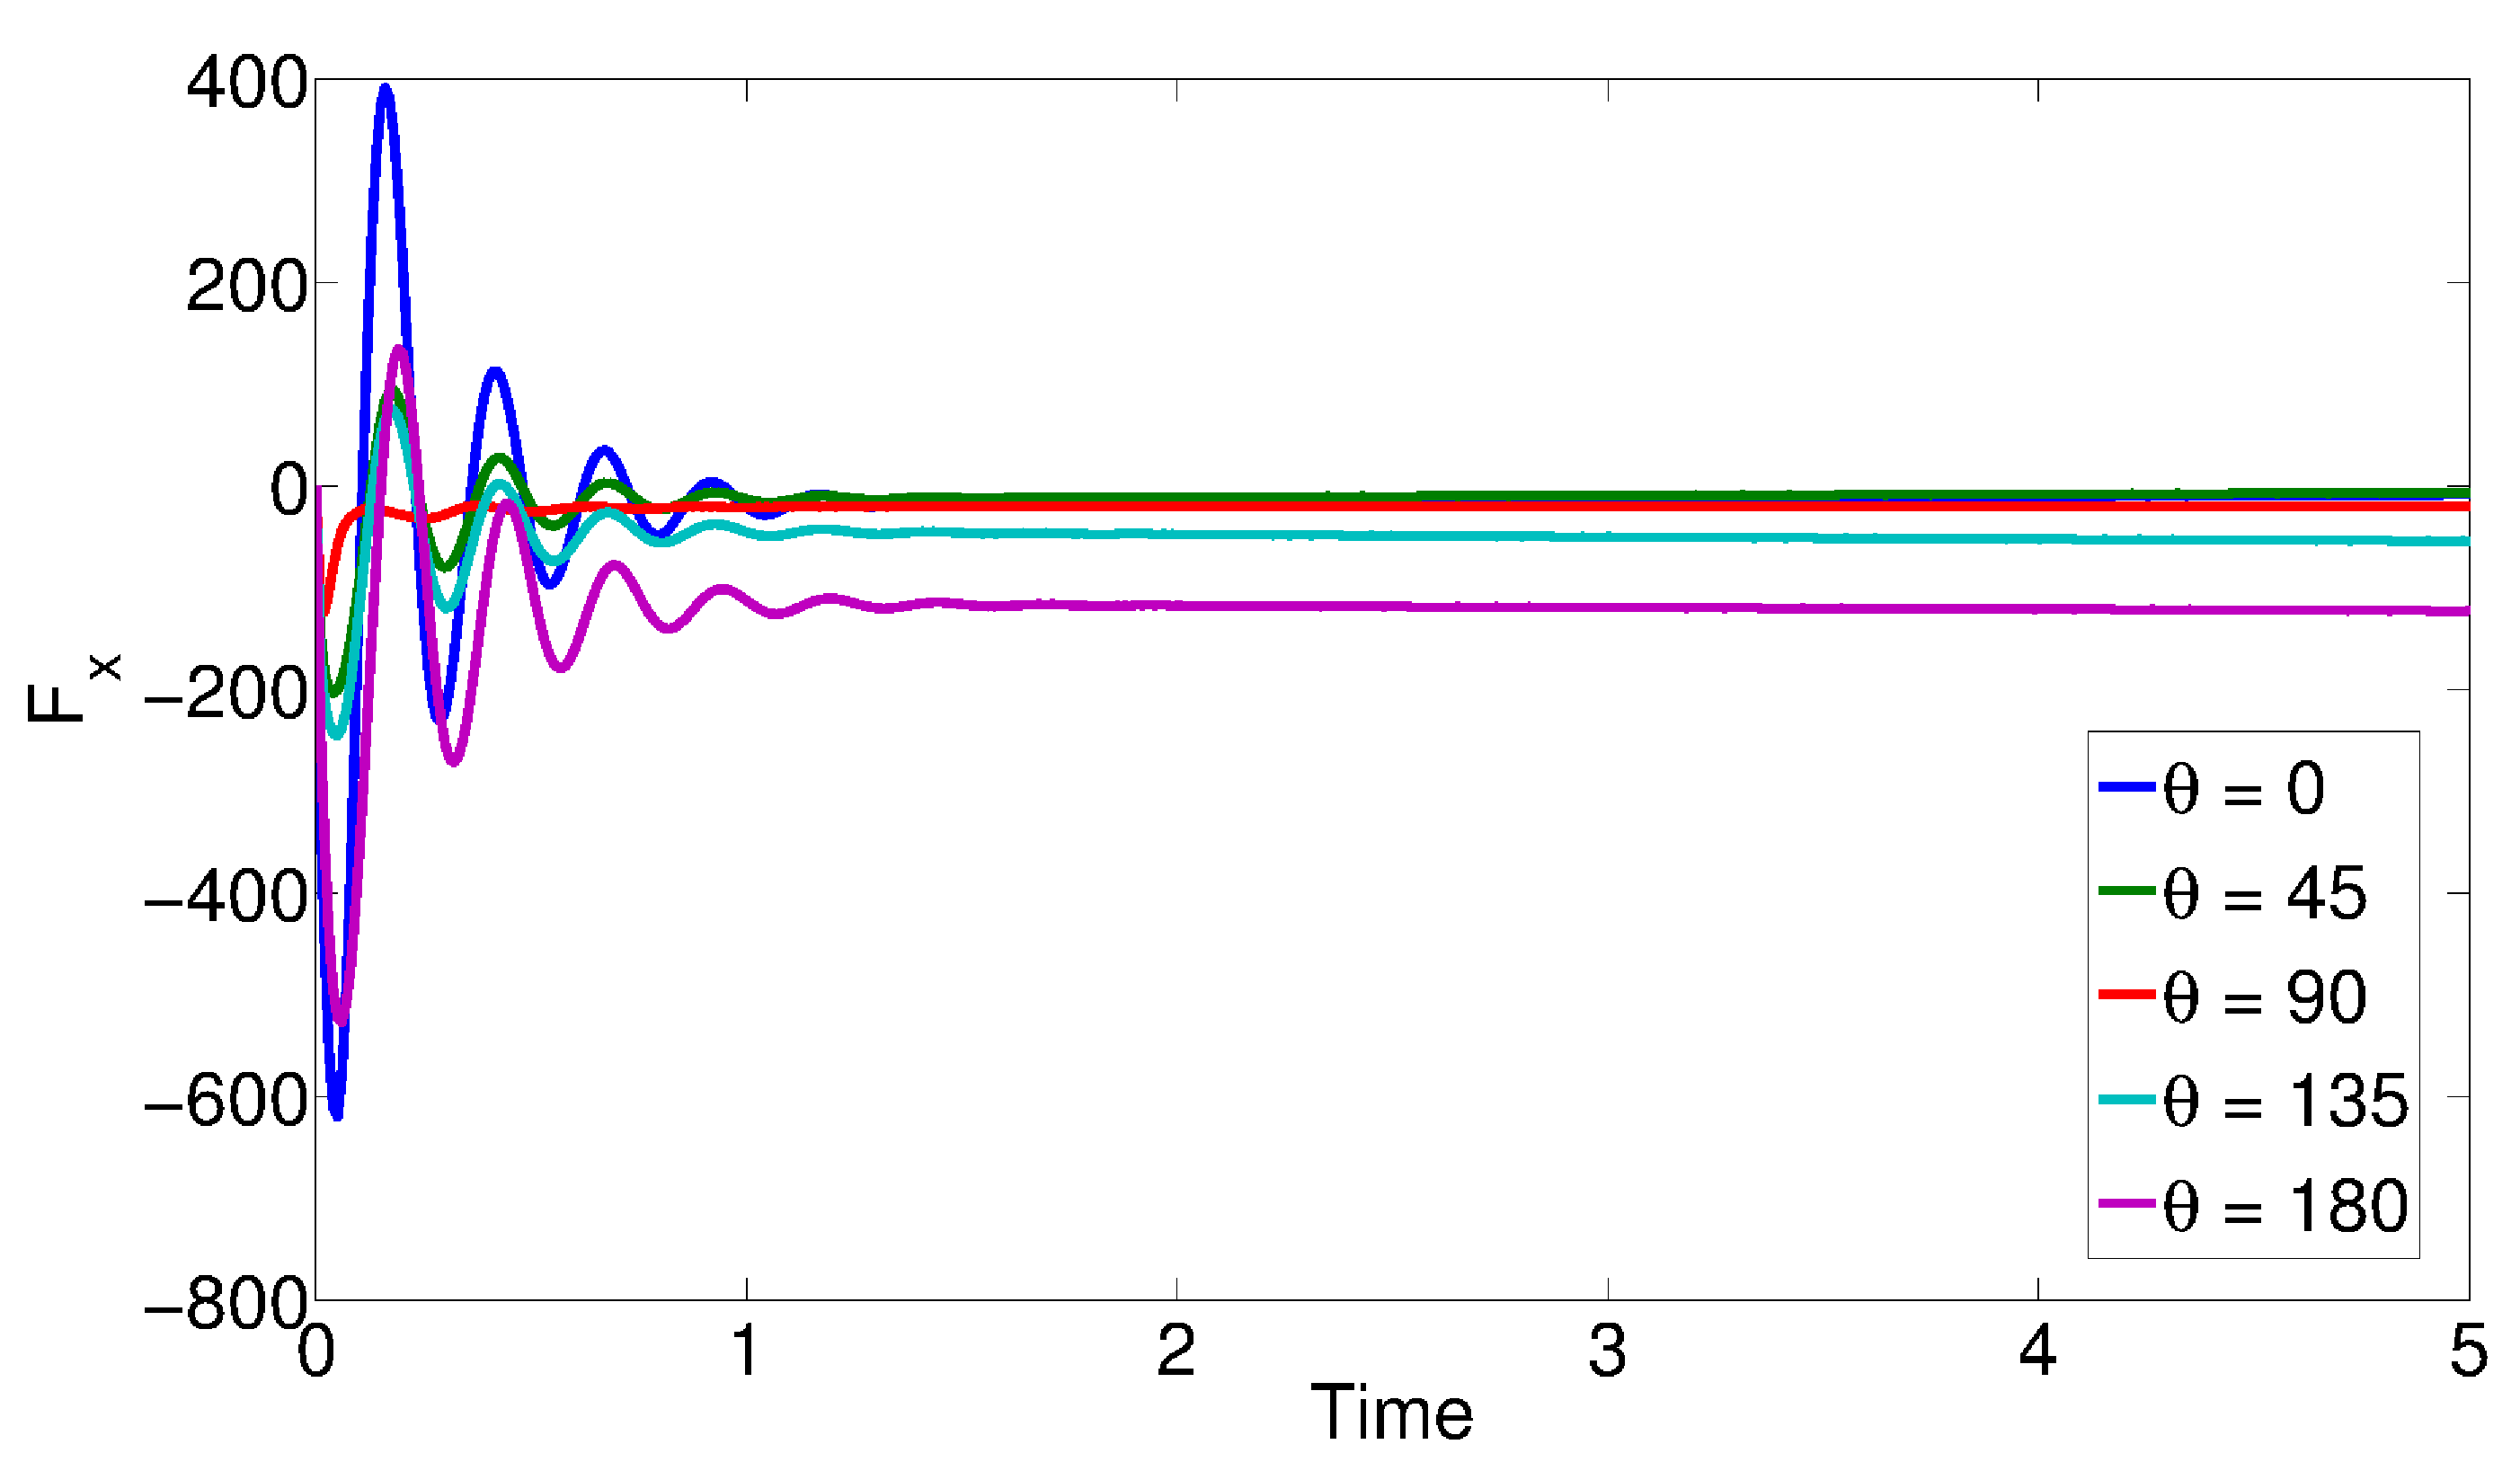
\includegraphics[height=4.15cm]{figure/cylinder/fx.eps}
	}
	\quad
	\subfigure[Forcing term in $y$ direction.]
	{
	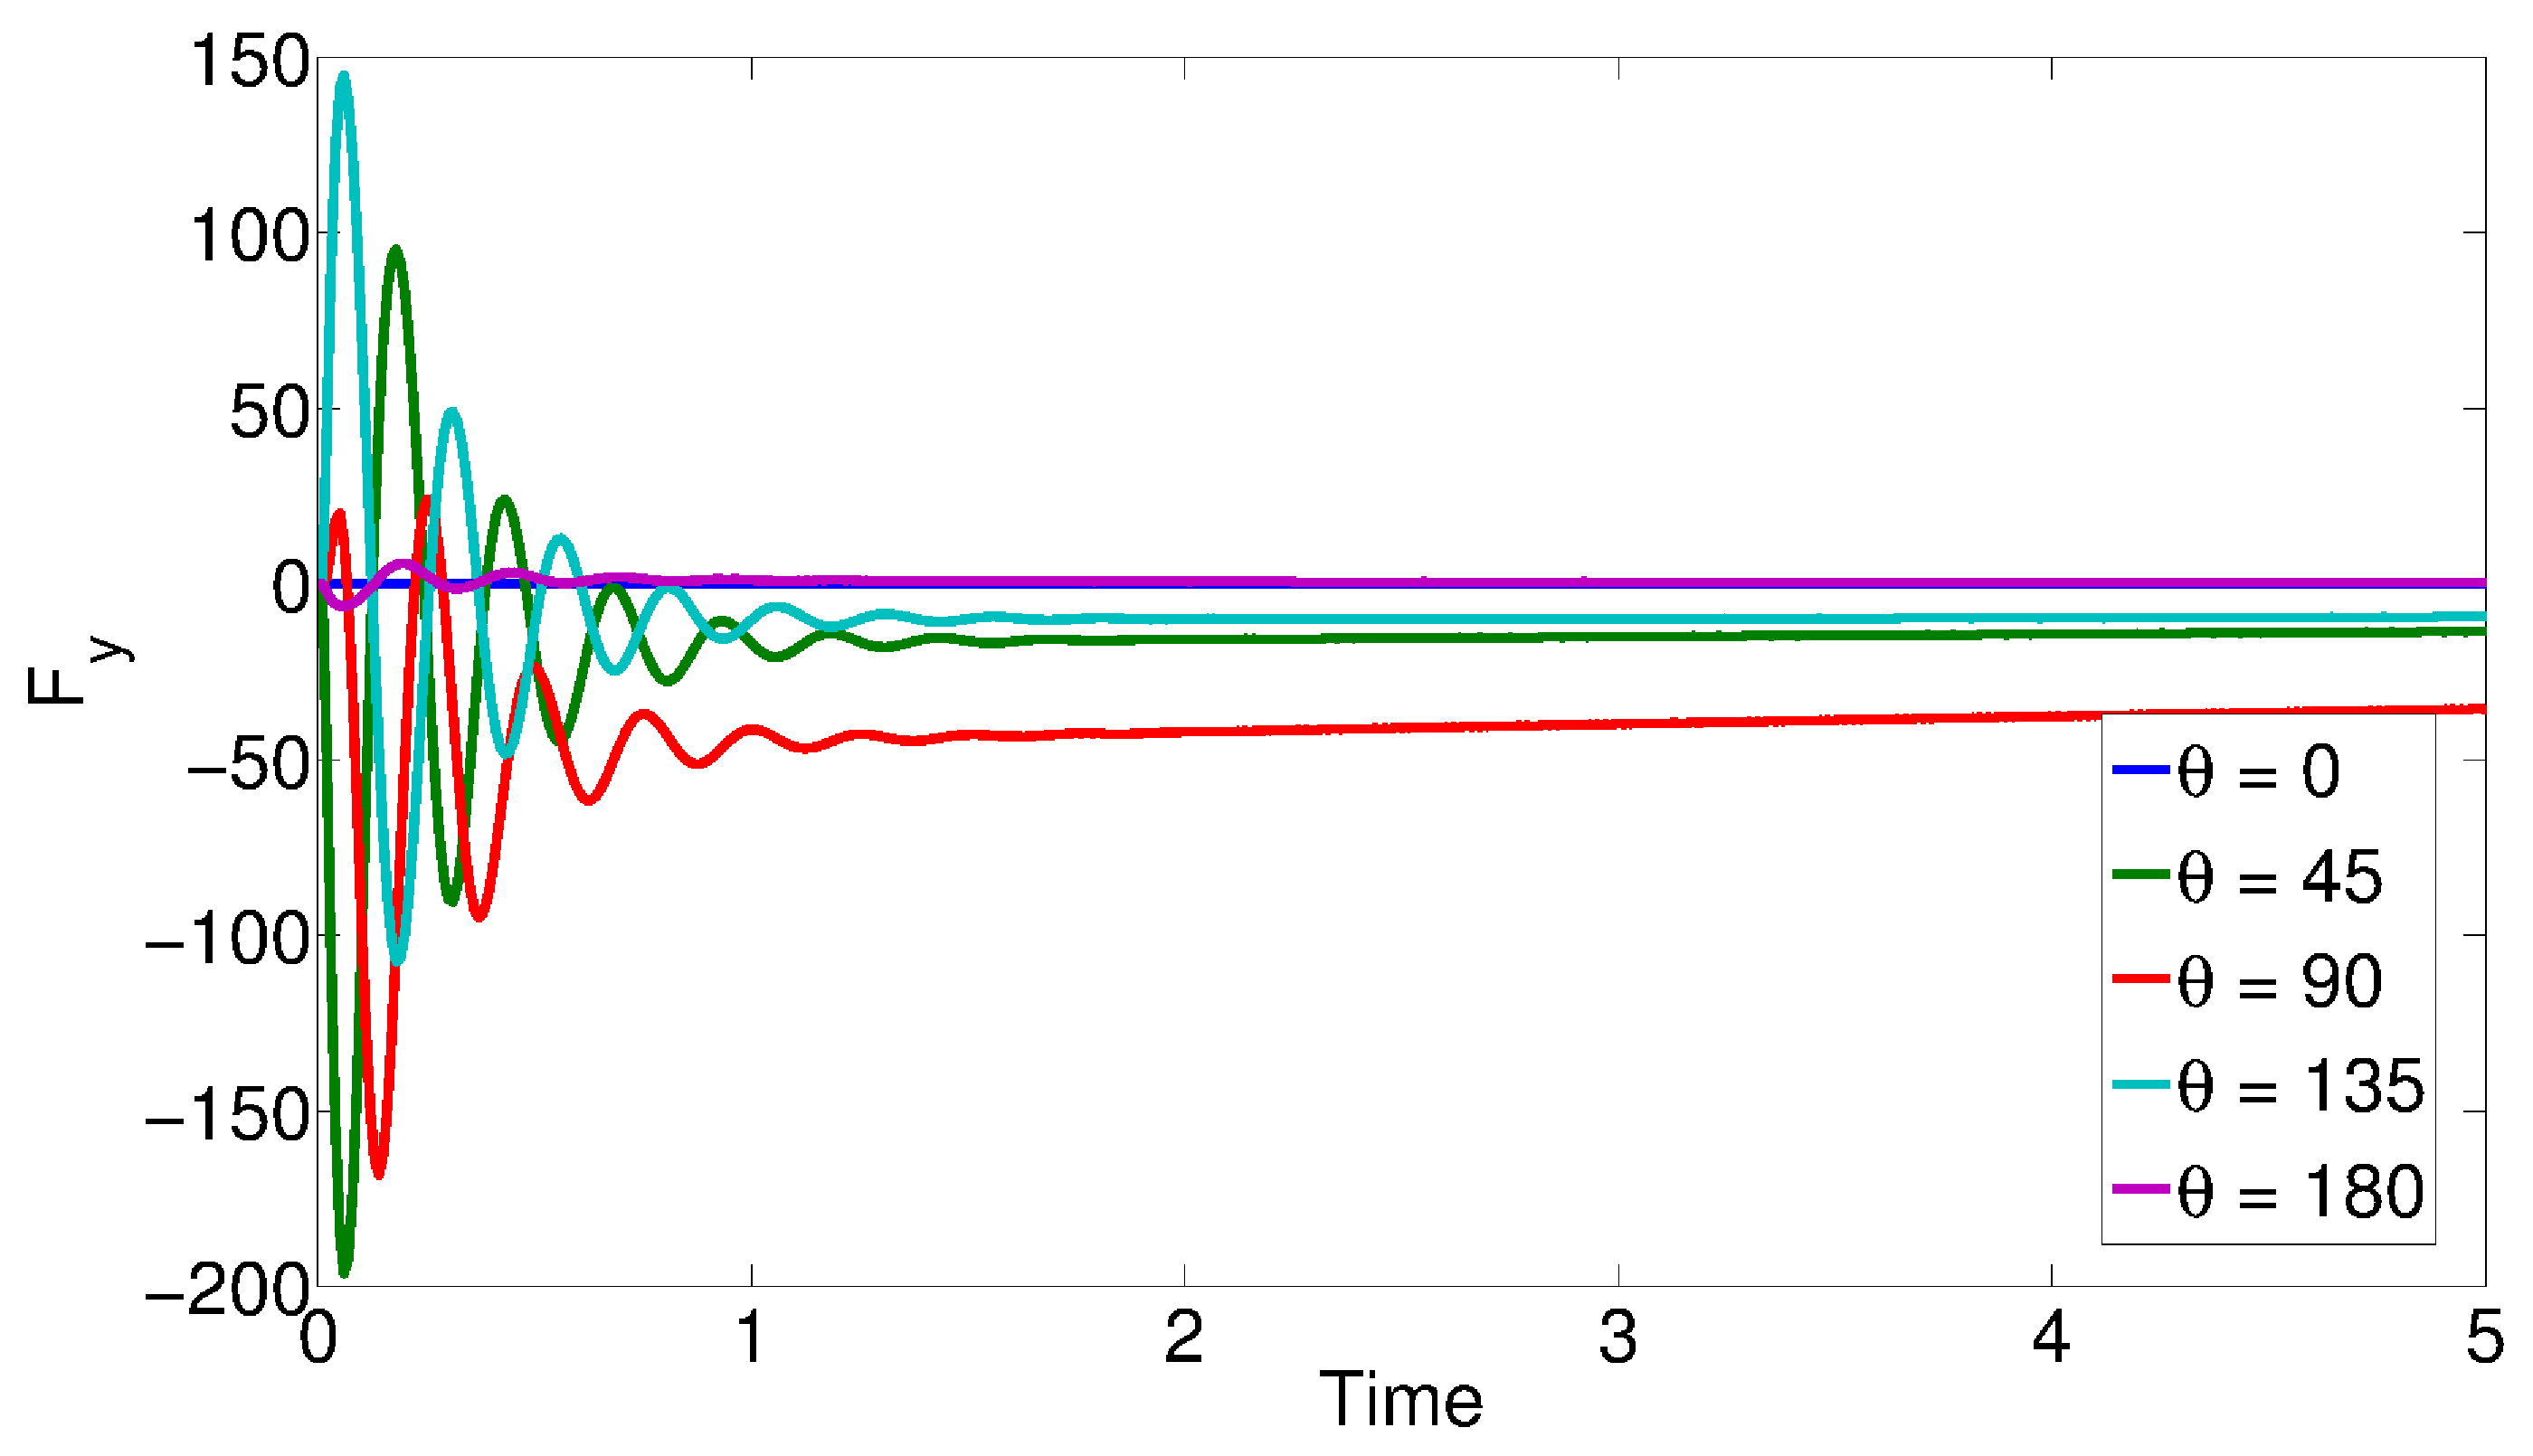
\includegraphics[height=4.15cm]{figure/cylinder/fy.eps}
	}
	\caption{Forcing terms on the cylinder surface. $\theta = 0$ is on the front and $\theta = 180$ is on the back of the cylinder for Re = 100.}
	\label{fig:cylinderForceTerms}
\end{figure}
%

The sensitivity contour plots for the pressure and velocity for different values of Reynolds numbers are shown in Figures \ref{fig:cylinderSensitivityContourRE100} and \ref{fig:cylinderSensitivityContourRE1000}. As shown here, the contour plots for the continuum sensitivity analysis and complex step results agree well with each other.

%
\begin{figure}[H]
	\centering
	\subfigure[Continuum sensitivity result for pressure]
	{
	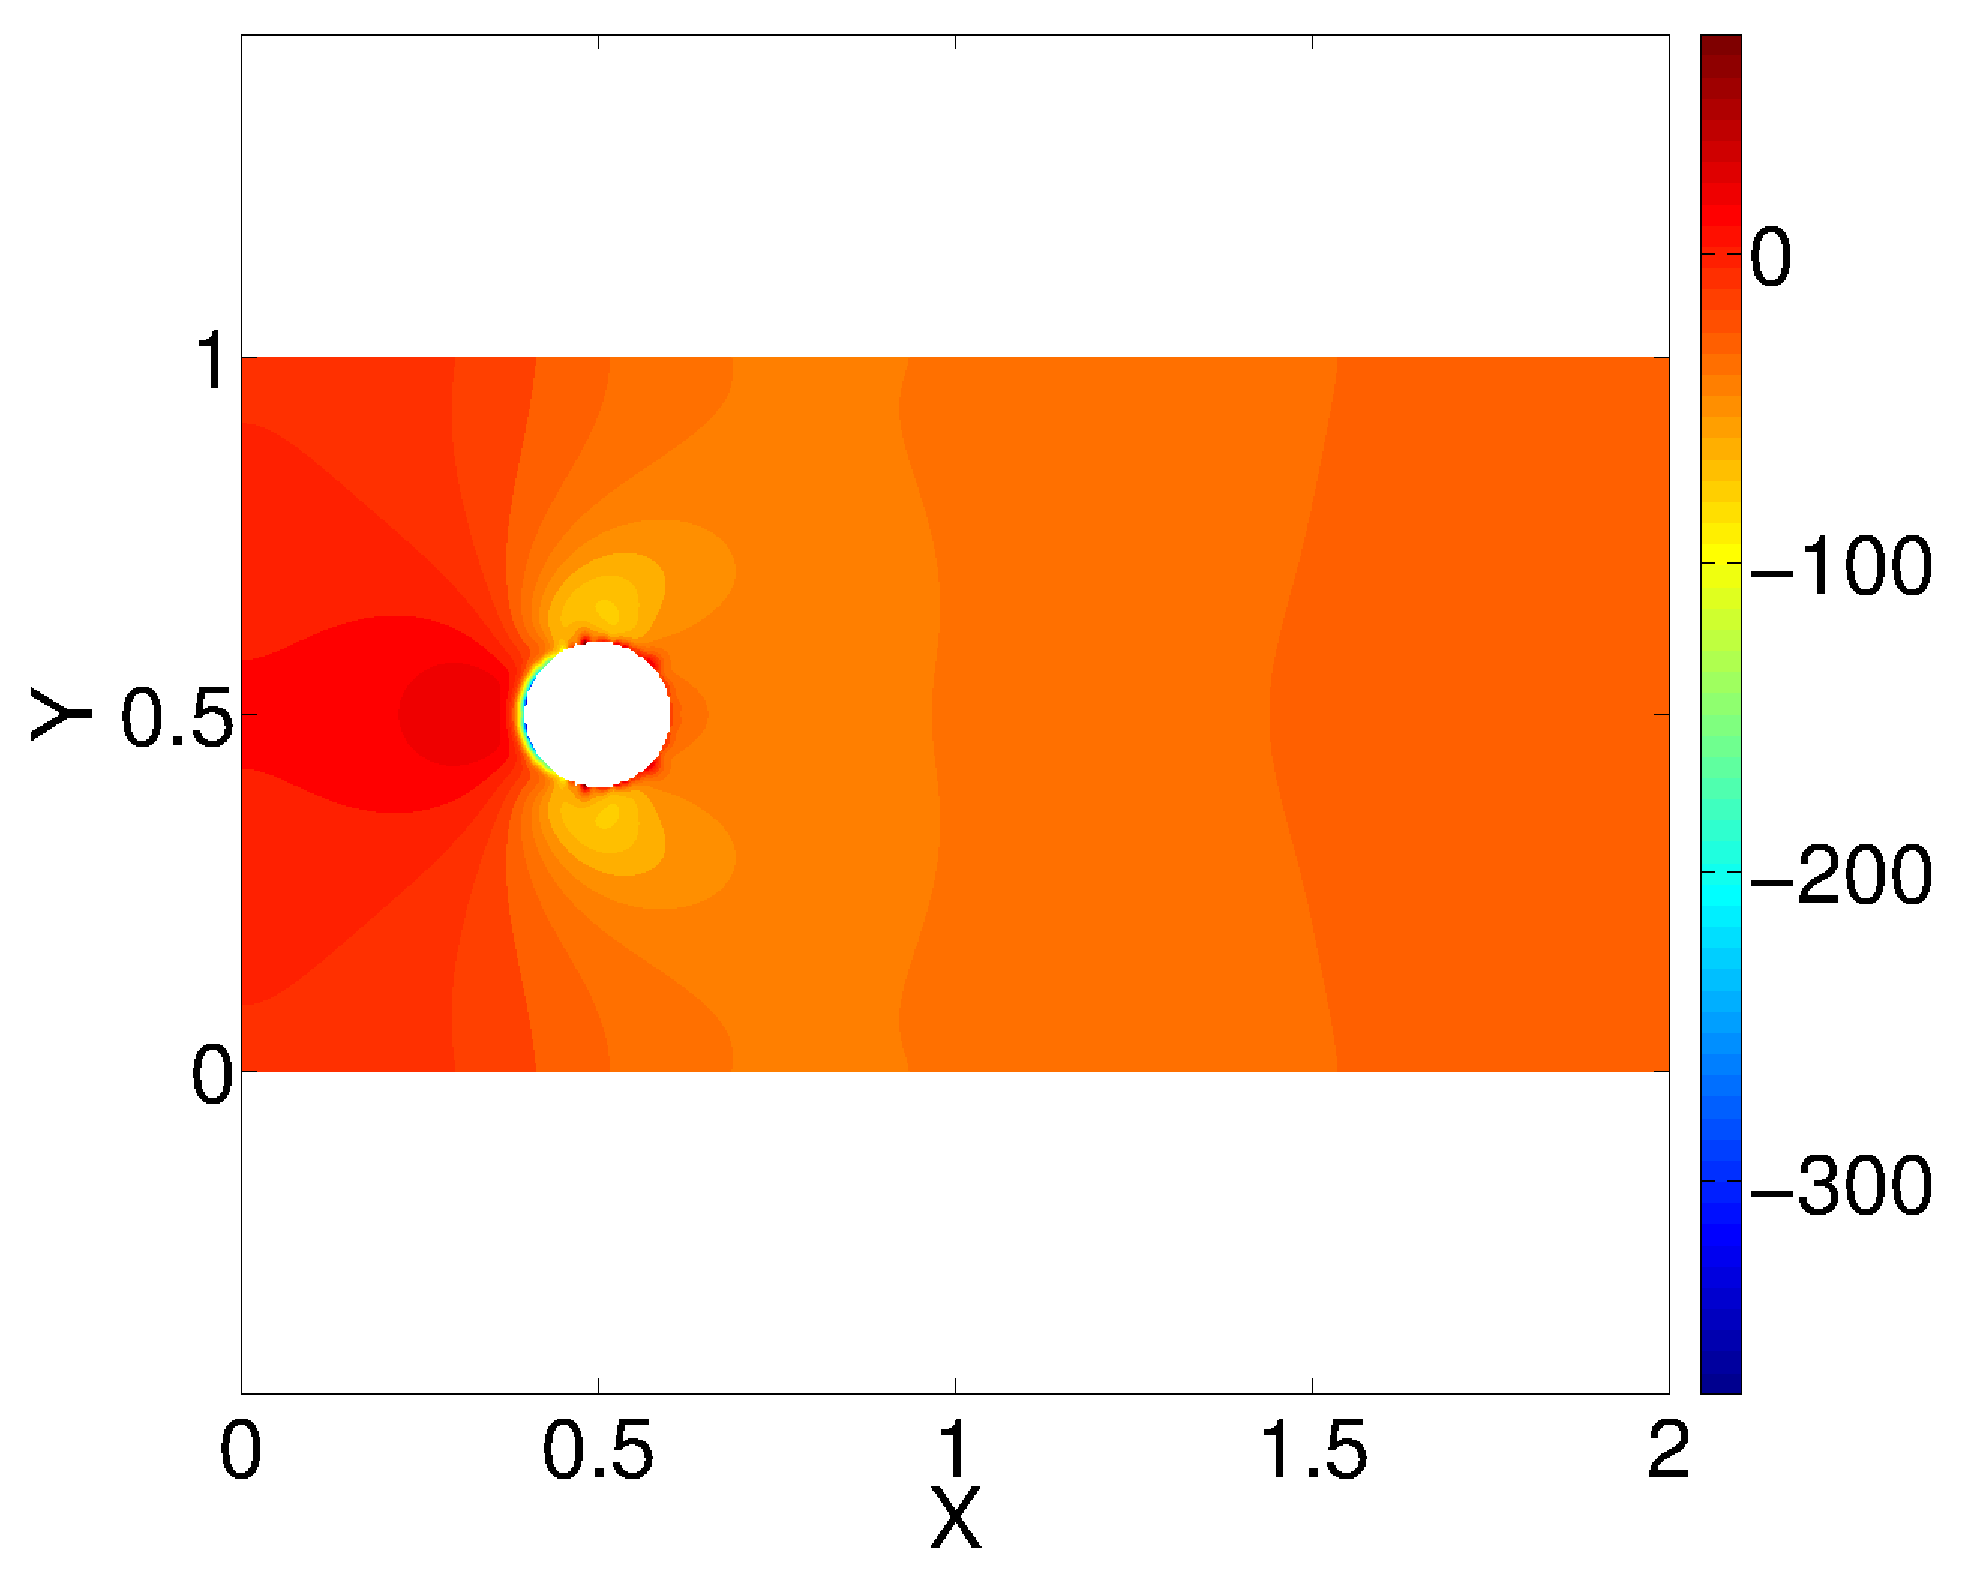
\includegraphics[height=6.0cm]{figure/cylinder/Pp_RE100.eps}
	}
	\quad
	\subfigure[Complex step result for pressure]
	{
	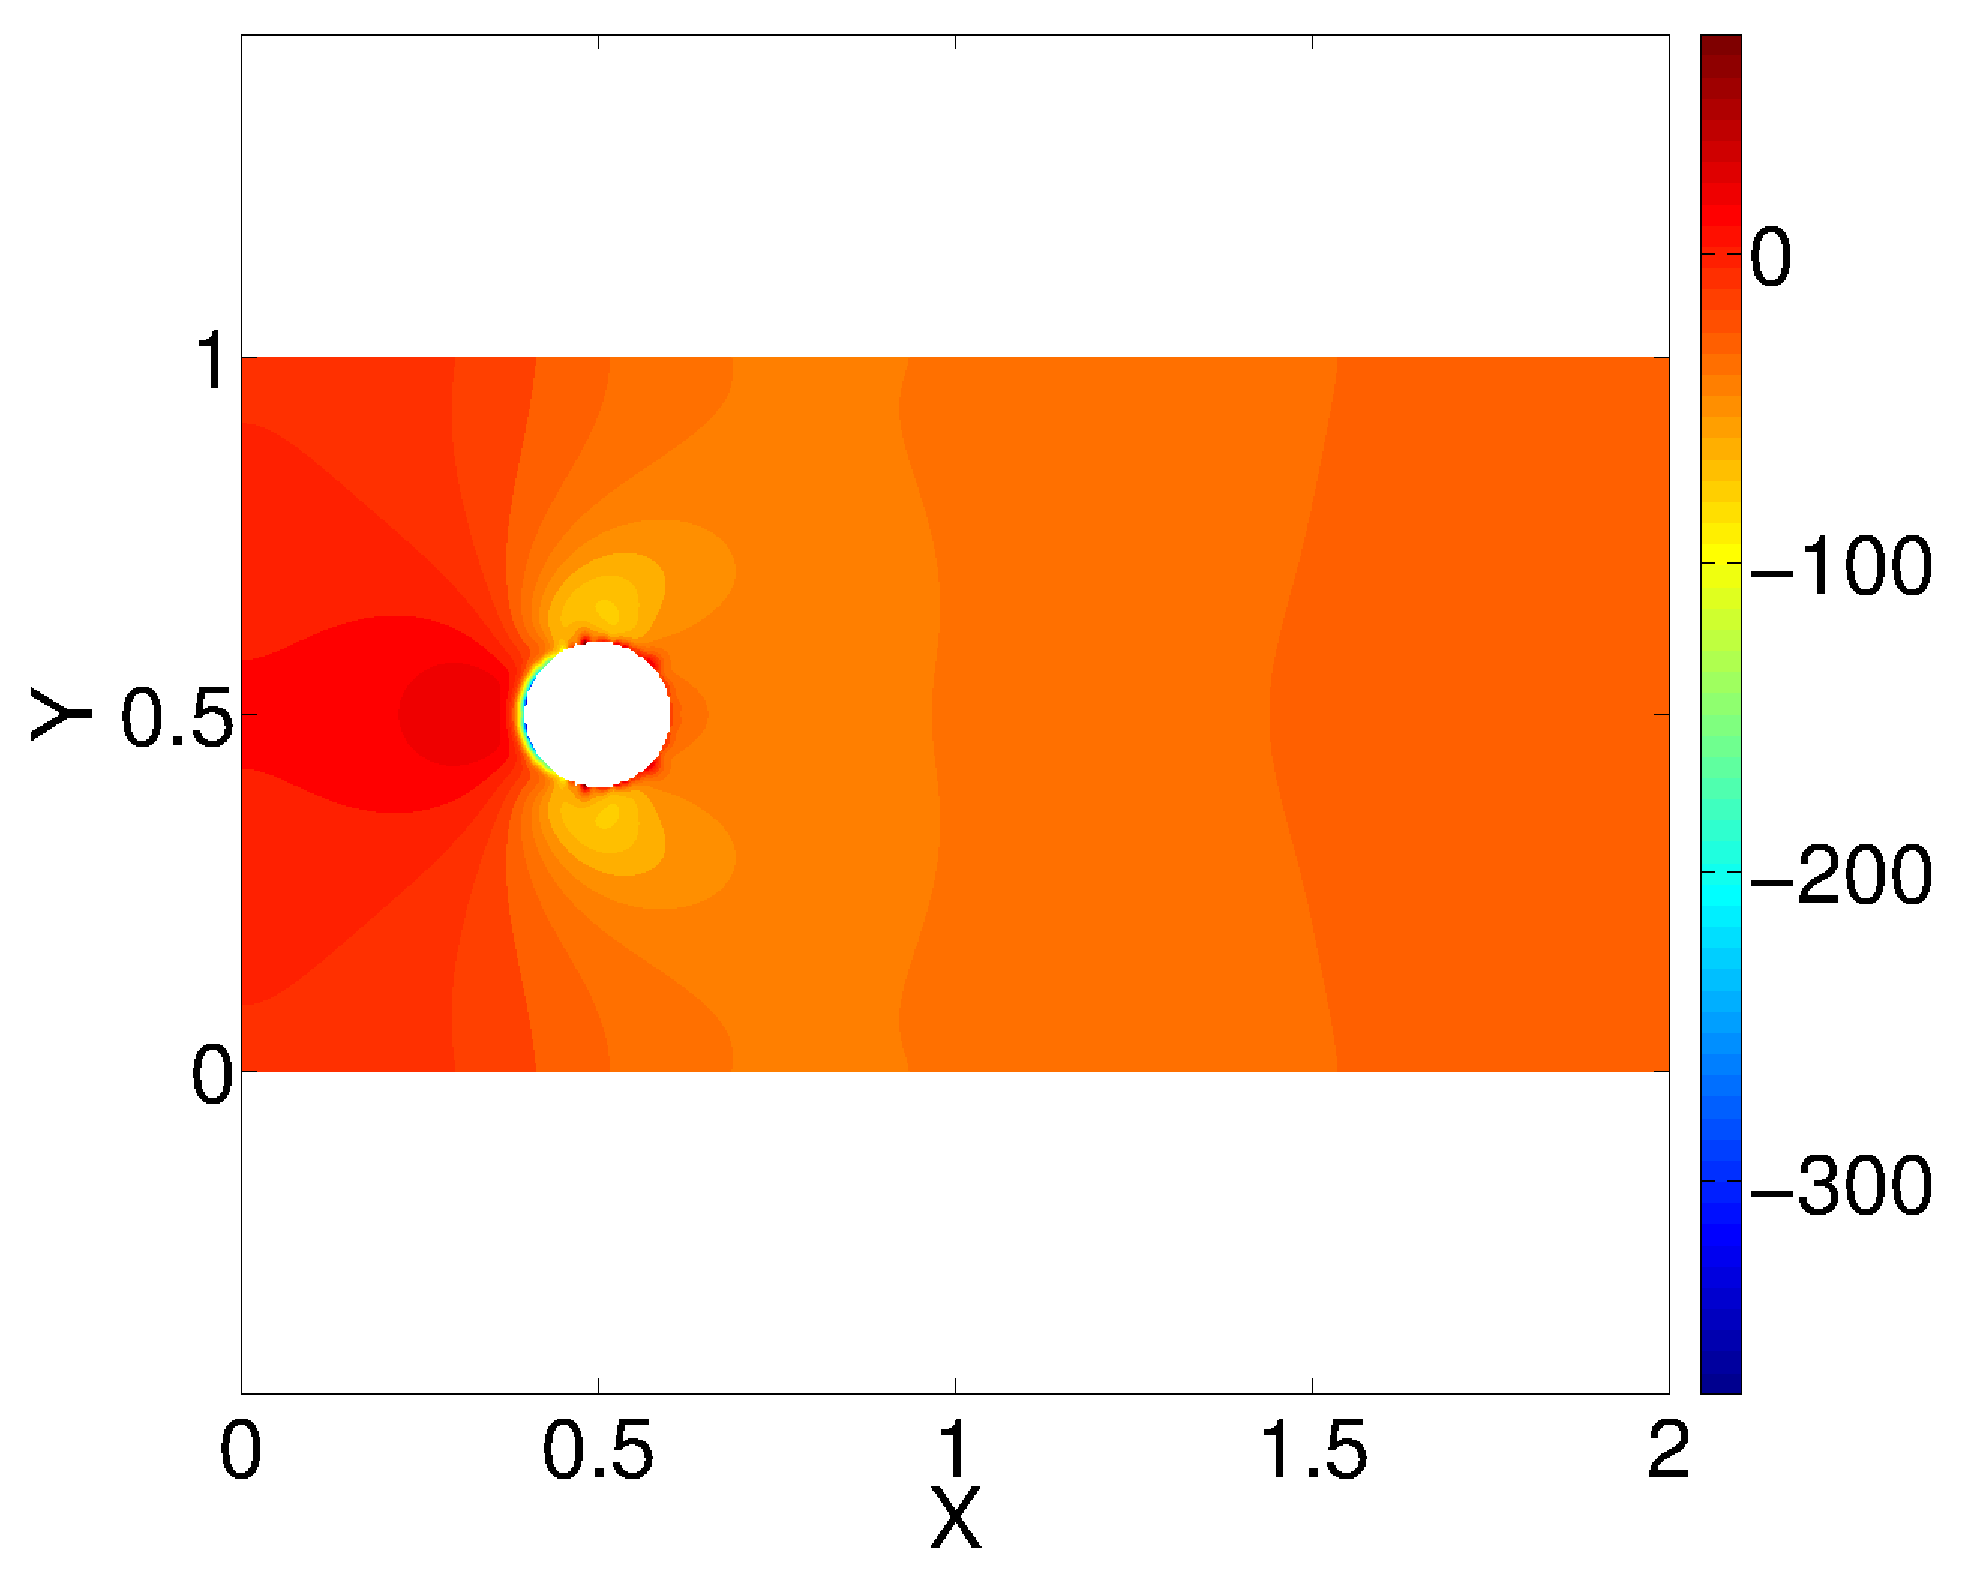
\includegraphics[height=6.0cm]{figure/cylinder/Pp_RE100.eps}
	}
	\\
	\subfigure[Continuum sensitivity result for u-velocity sensitivity]
	{
	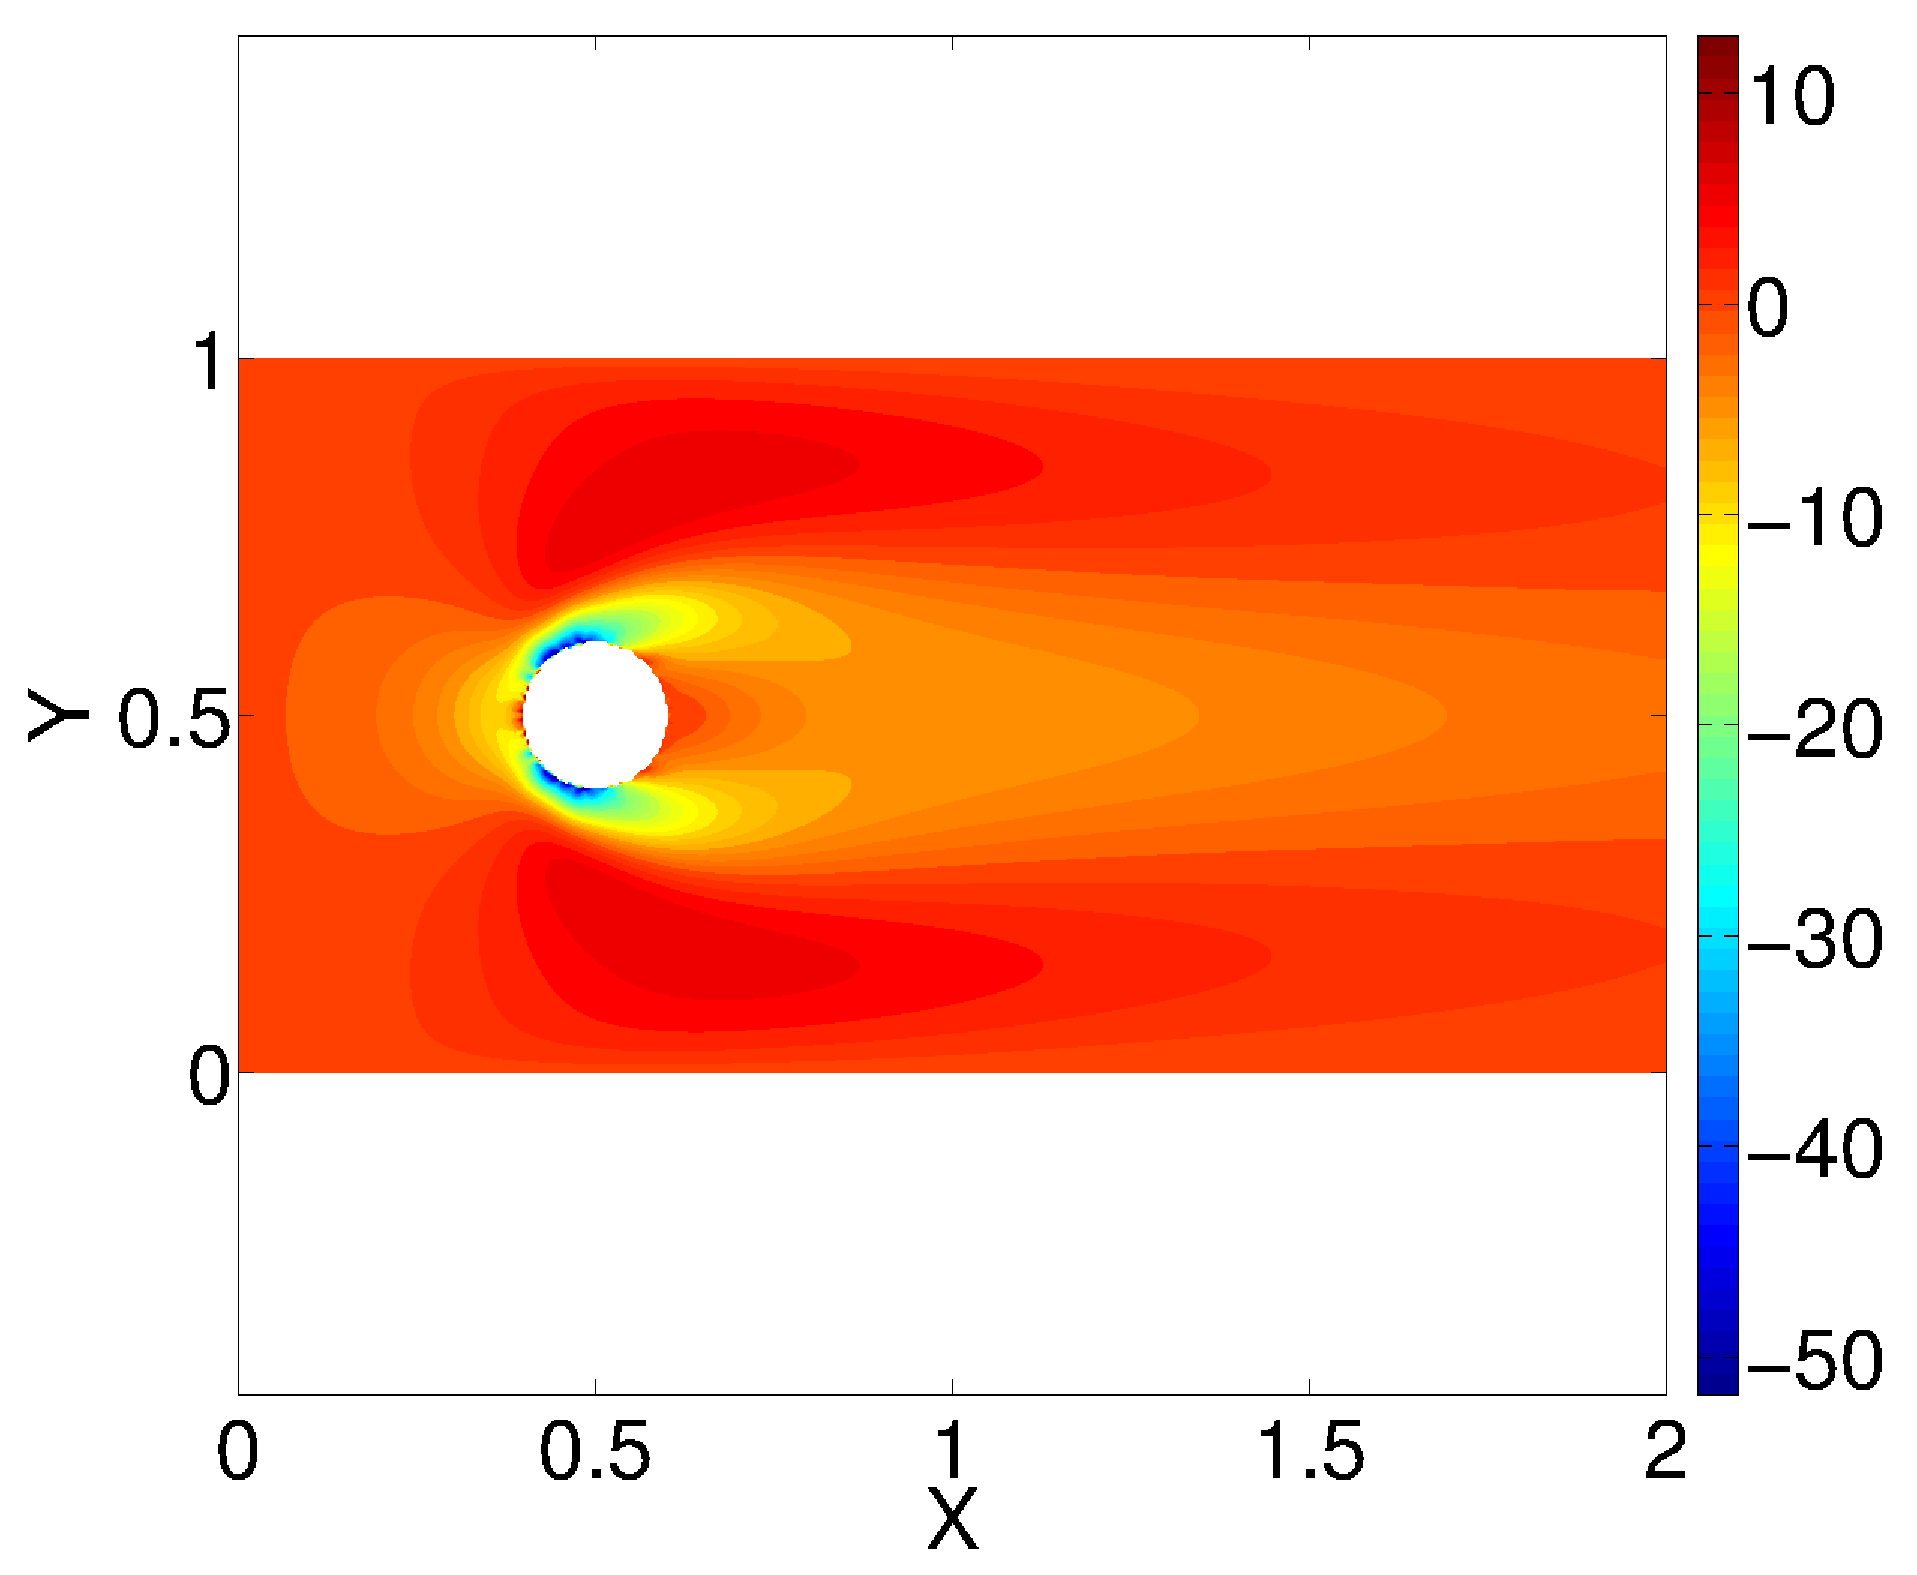
\includegraphics[height=6.0cm]{figure/cylinder/Up_RE100.eps}
	}
	\quad
	\subfigure[Complex step result for u-velocity]
	{
	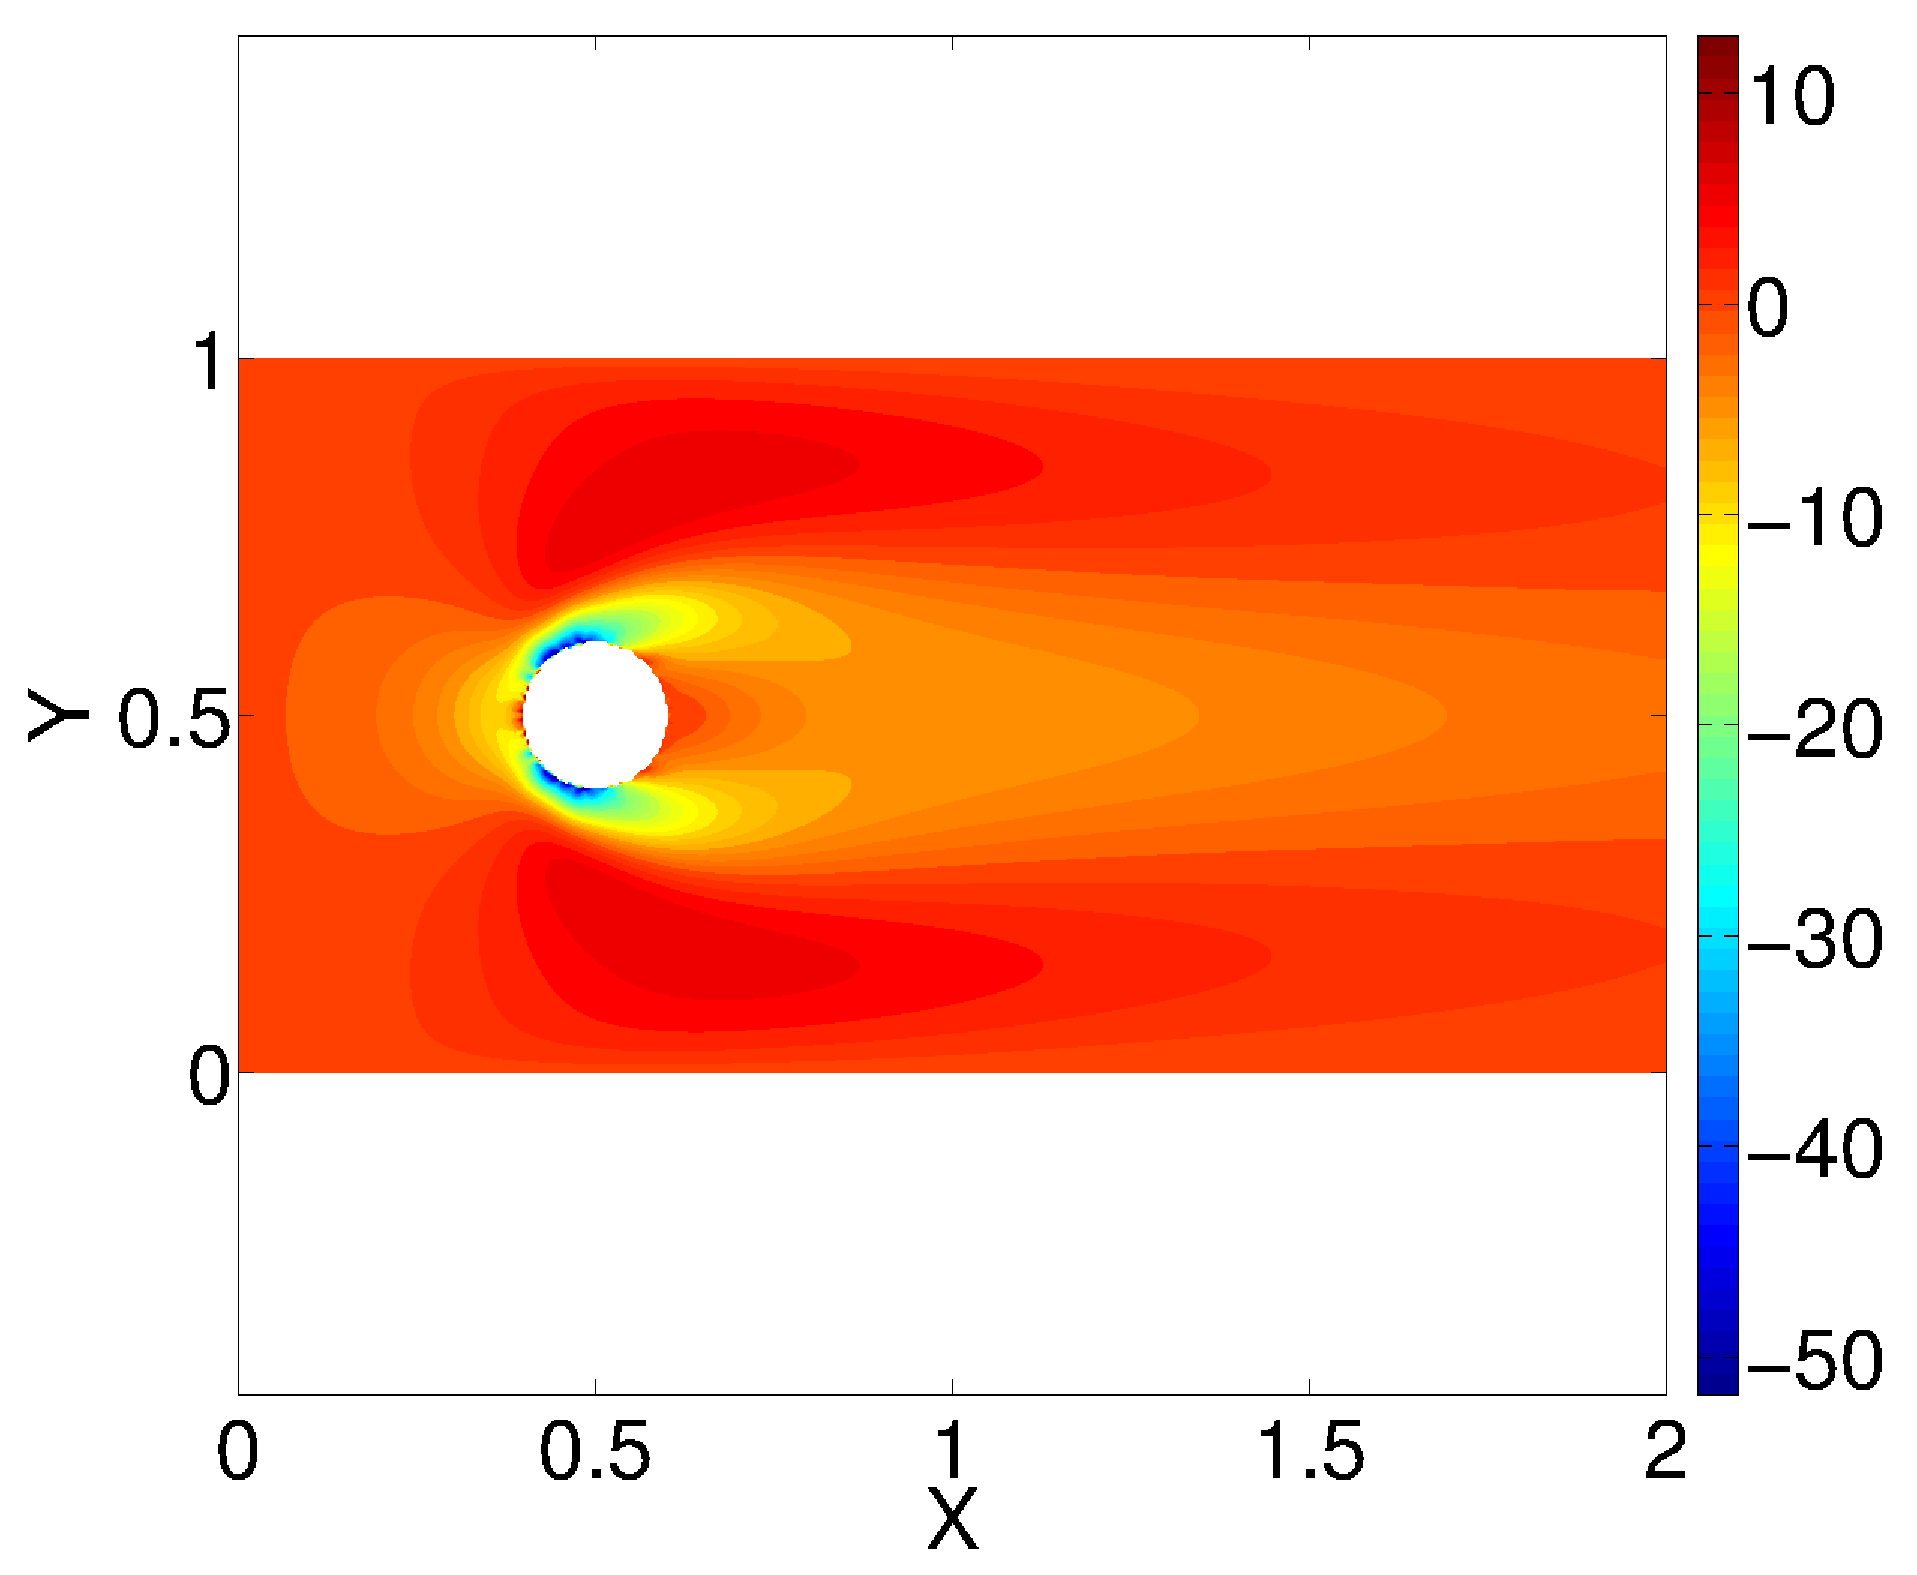
\includegraphics[height=6.0cm]{figure/cylinder/Up_RE100.eps}
	}
	\\
	\subfigure[Continuum sensitivity result for v-velocity]
	{
	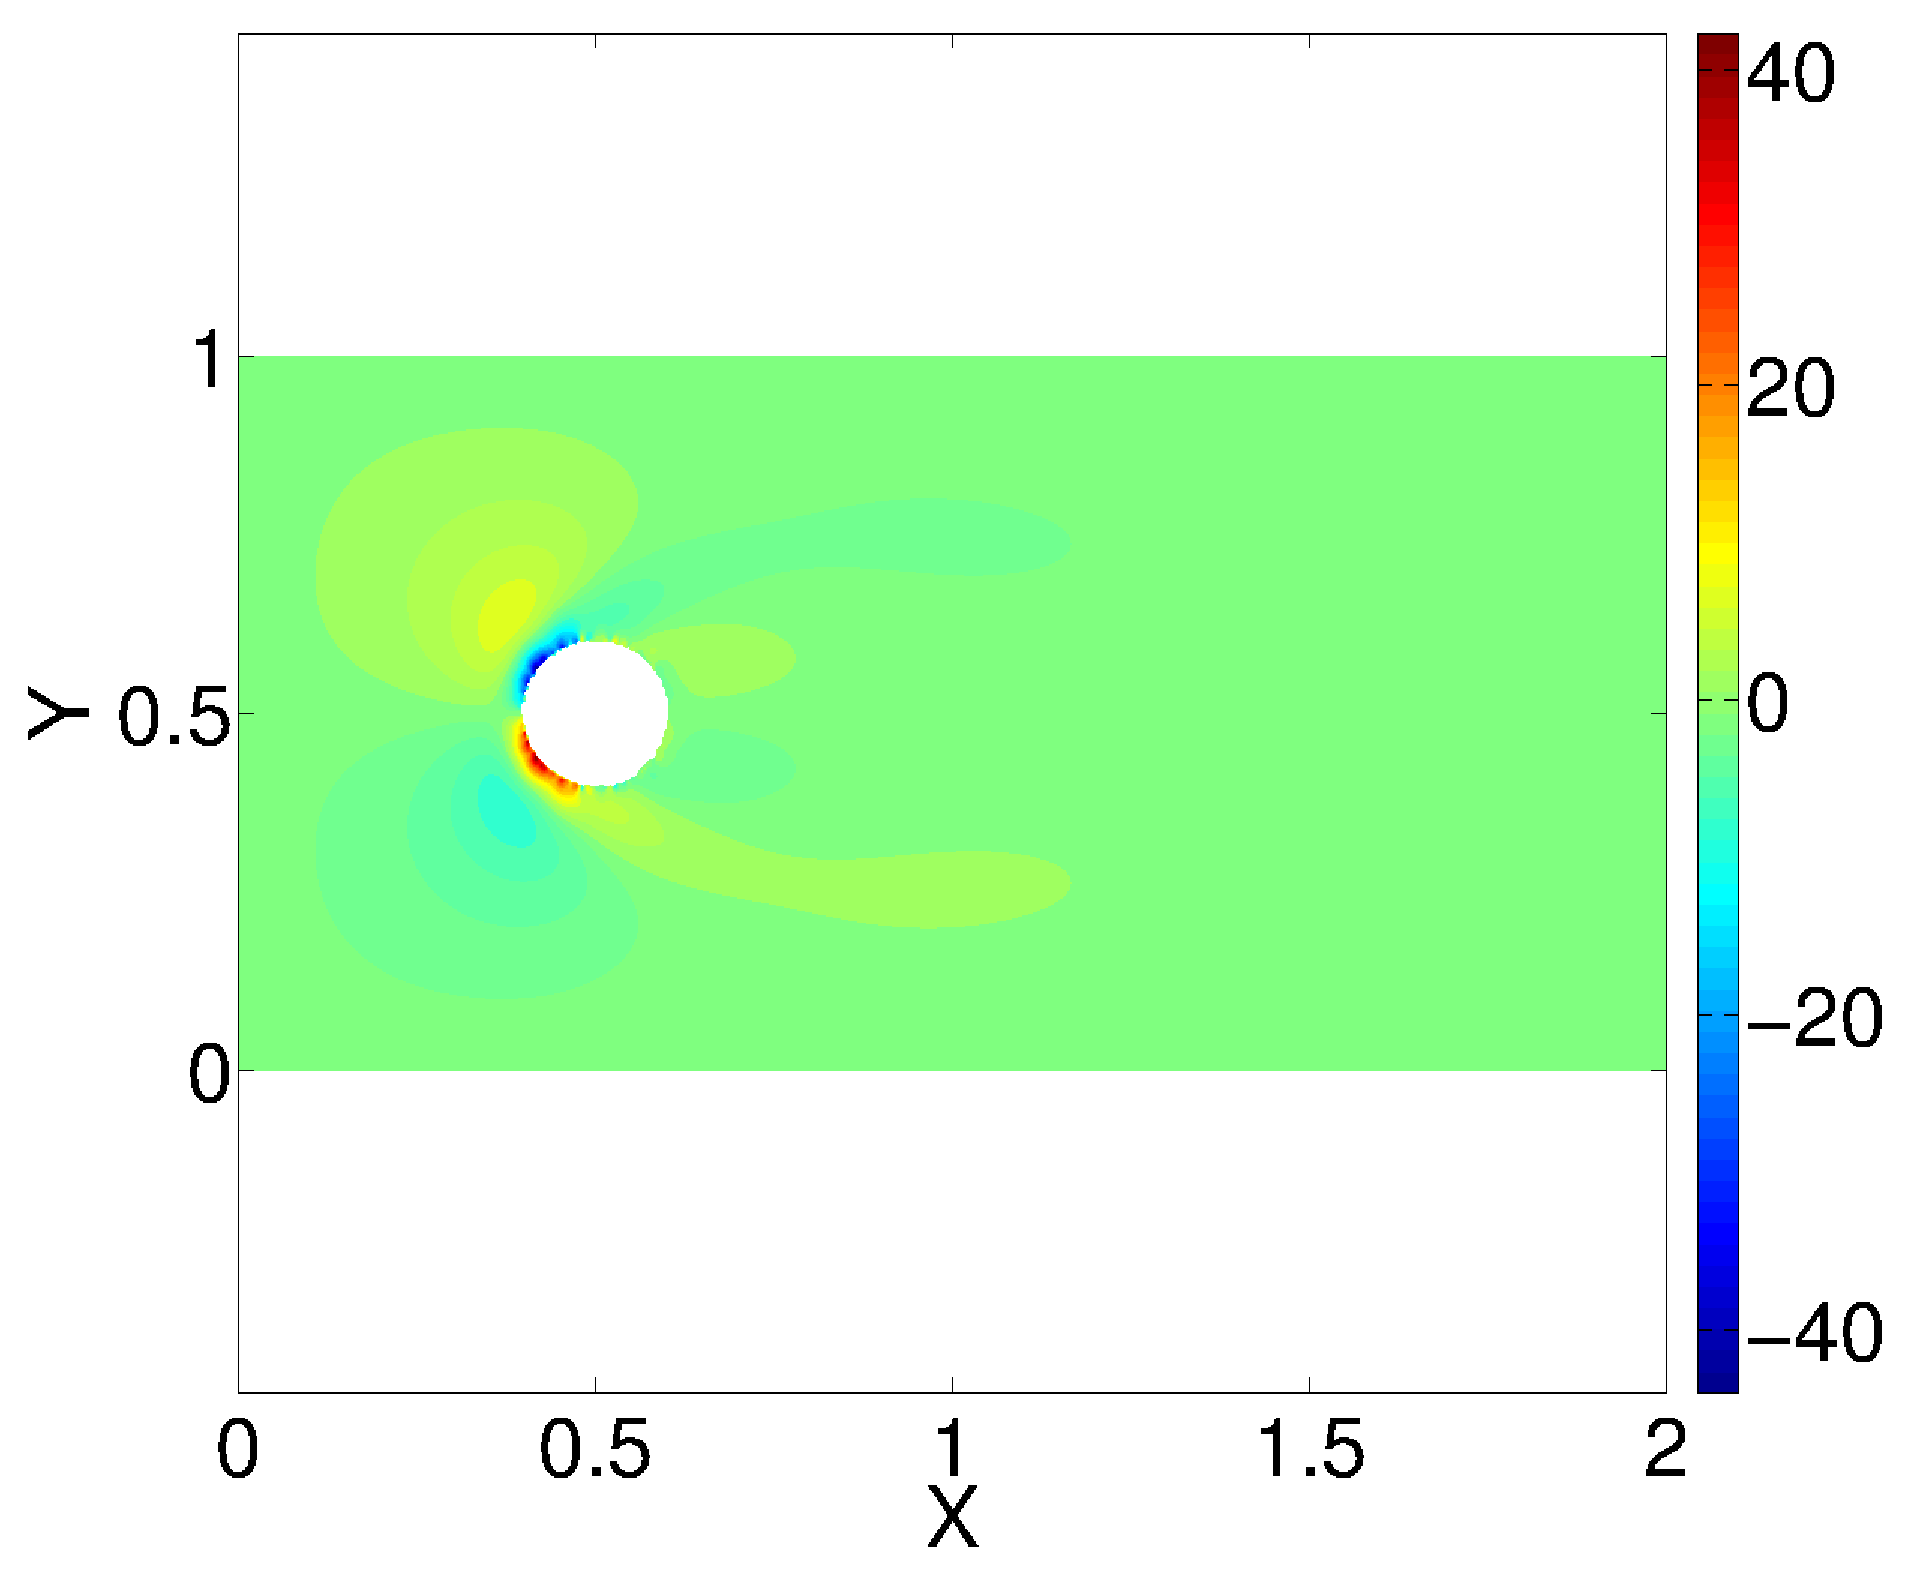
\includegraphics[height=6.0cm]{figure/cylinder/Vp_RE100.eps}
	}
	\quad
	\subfigure[Complex step result for v-velocity]
	{
	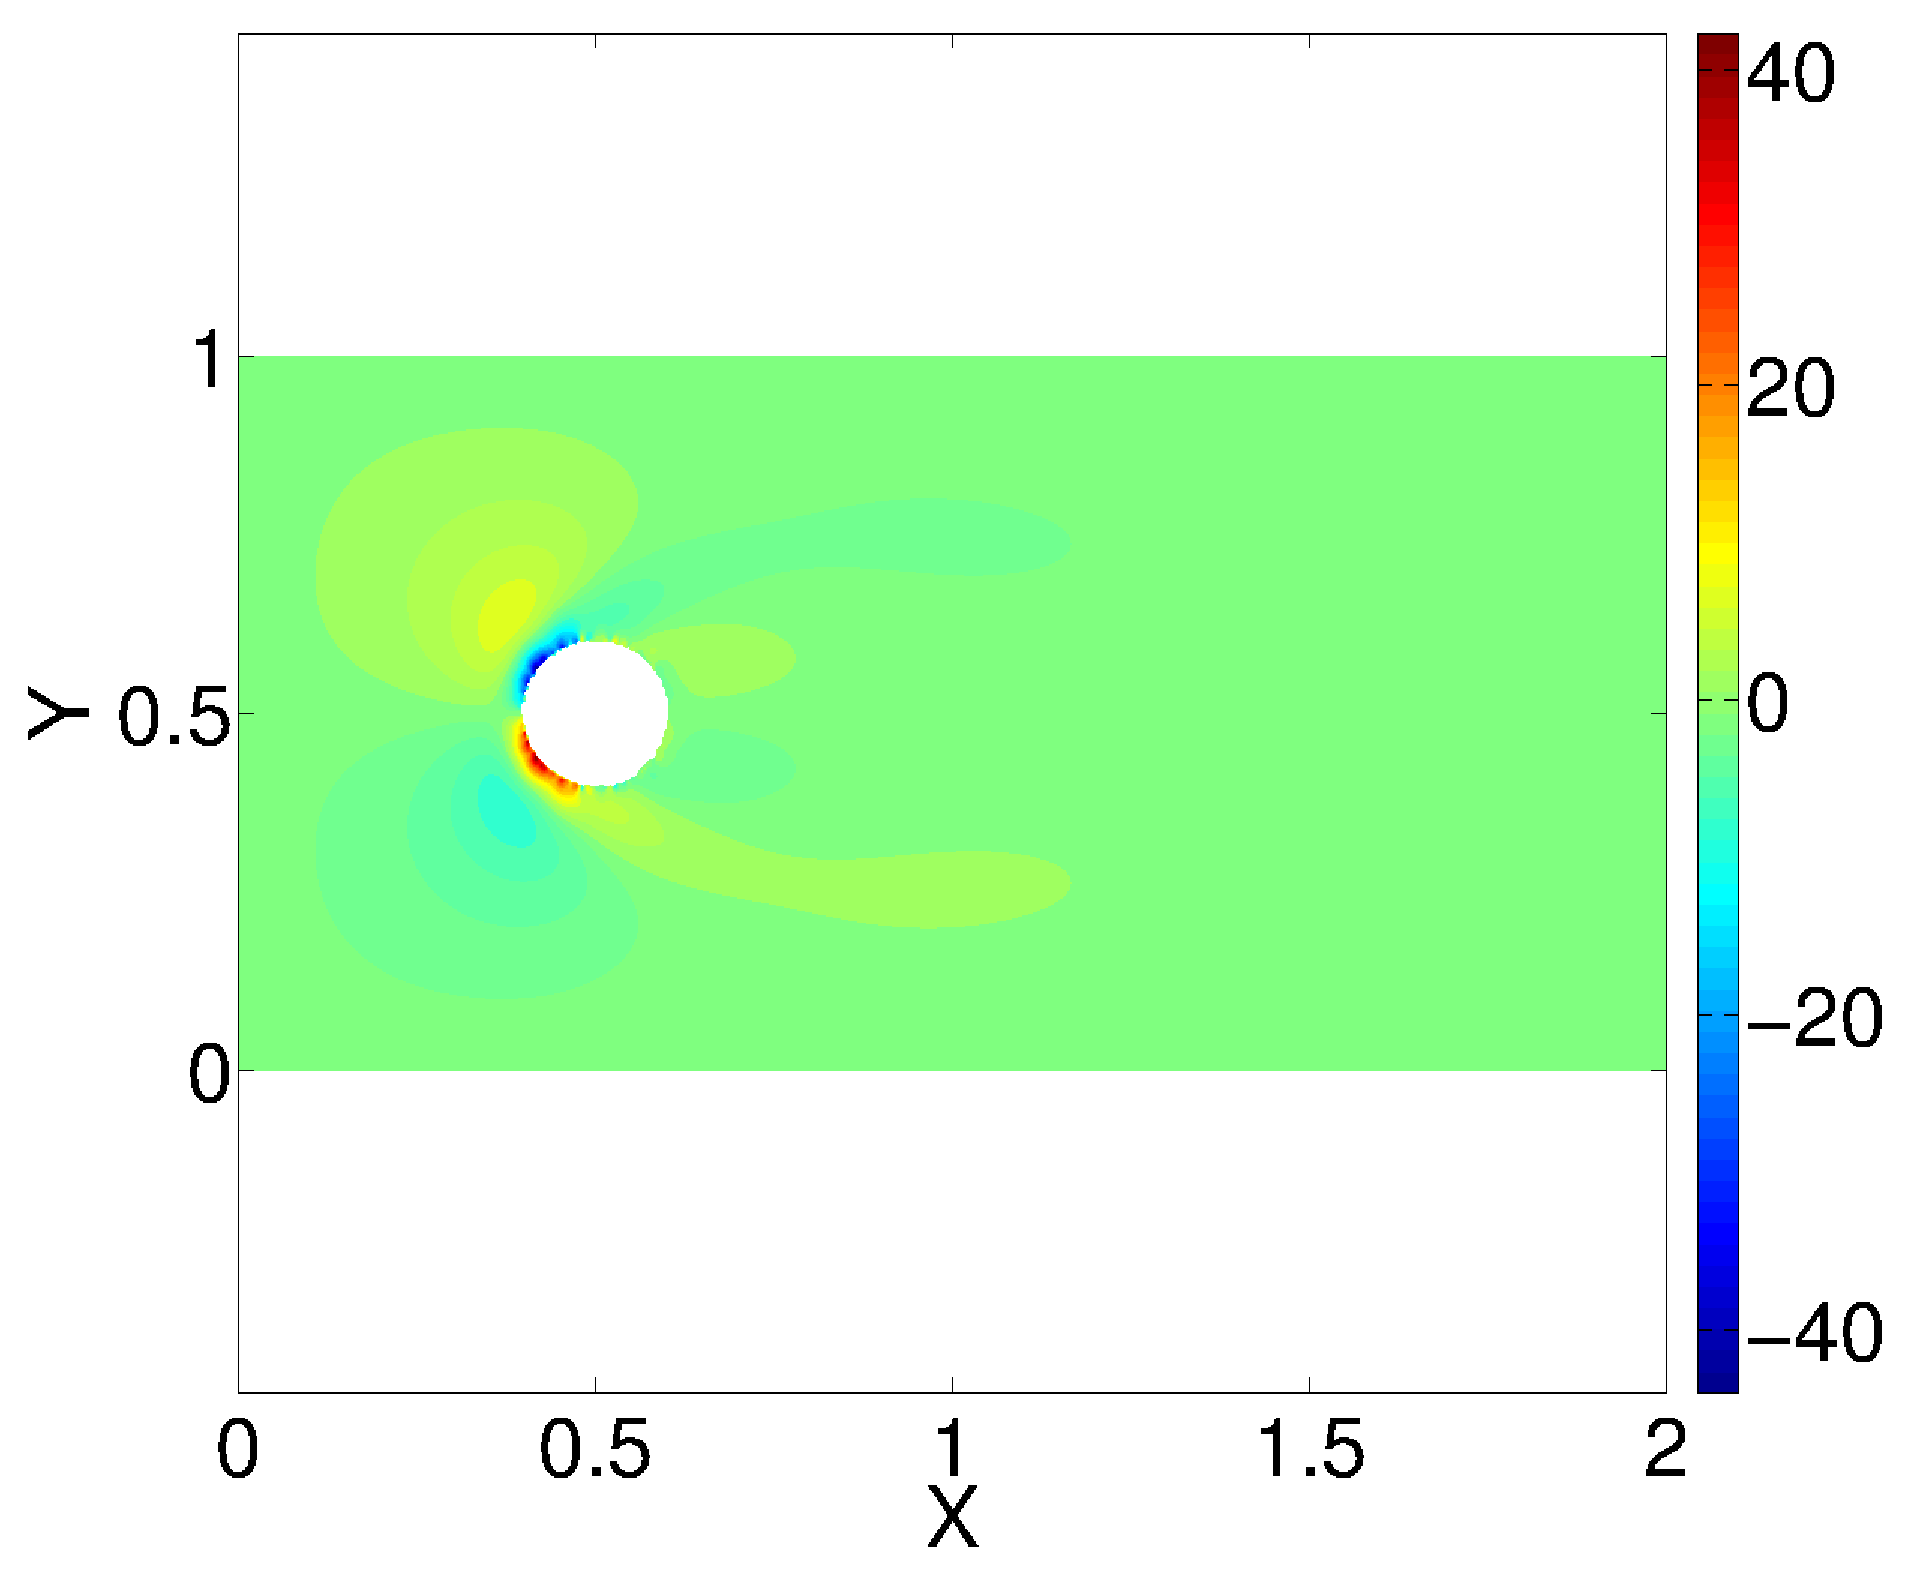
\includegraphics[height=6.0cm]{figure/cylinder/Vp_RE100.eps}
	}
	\caption{Comparison of sensitivity contours for flow over cylinder, $Re = 100$.}
	\label{fig:cylinderSensitivityContourRE100}
\end{figure}
%

%
\begin{figure}[H]
	\centering
	\subfigure[Continuum sensitivity result for pressure]
	{
	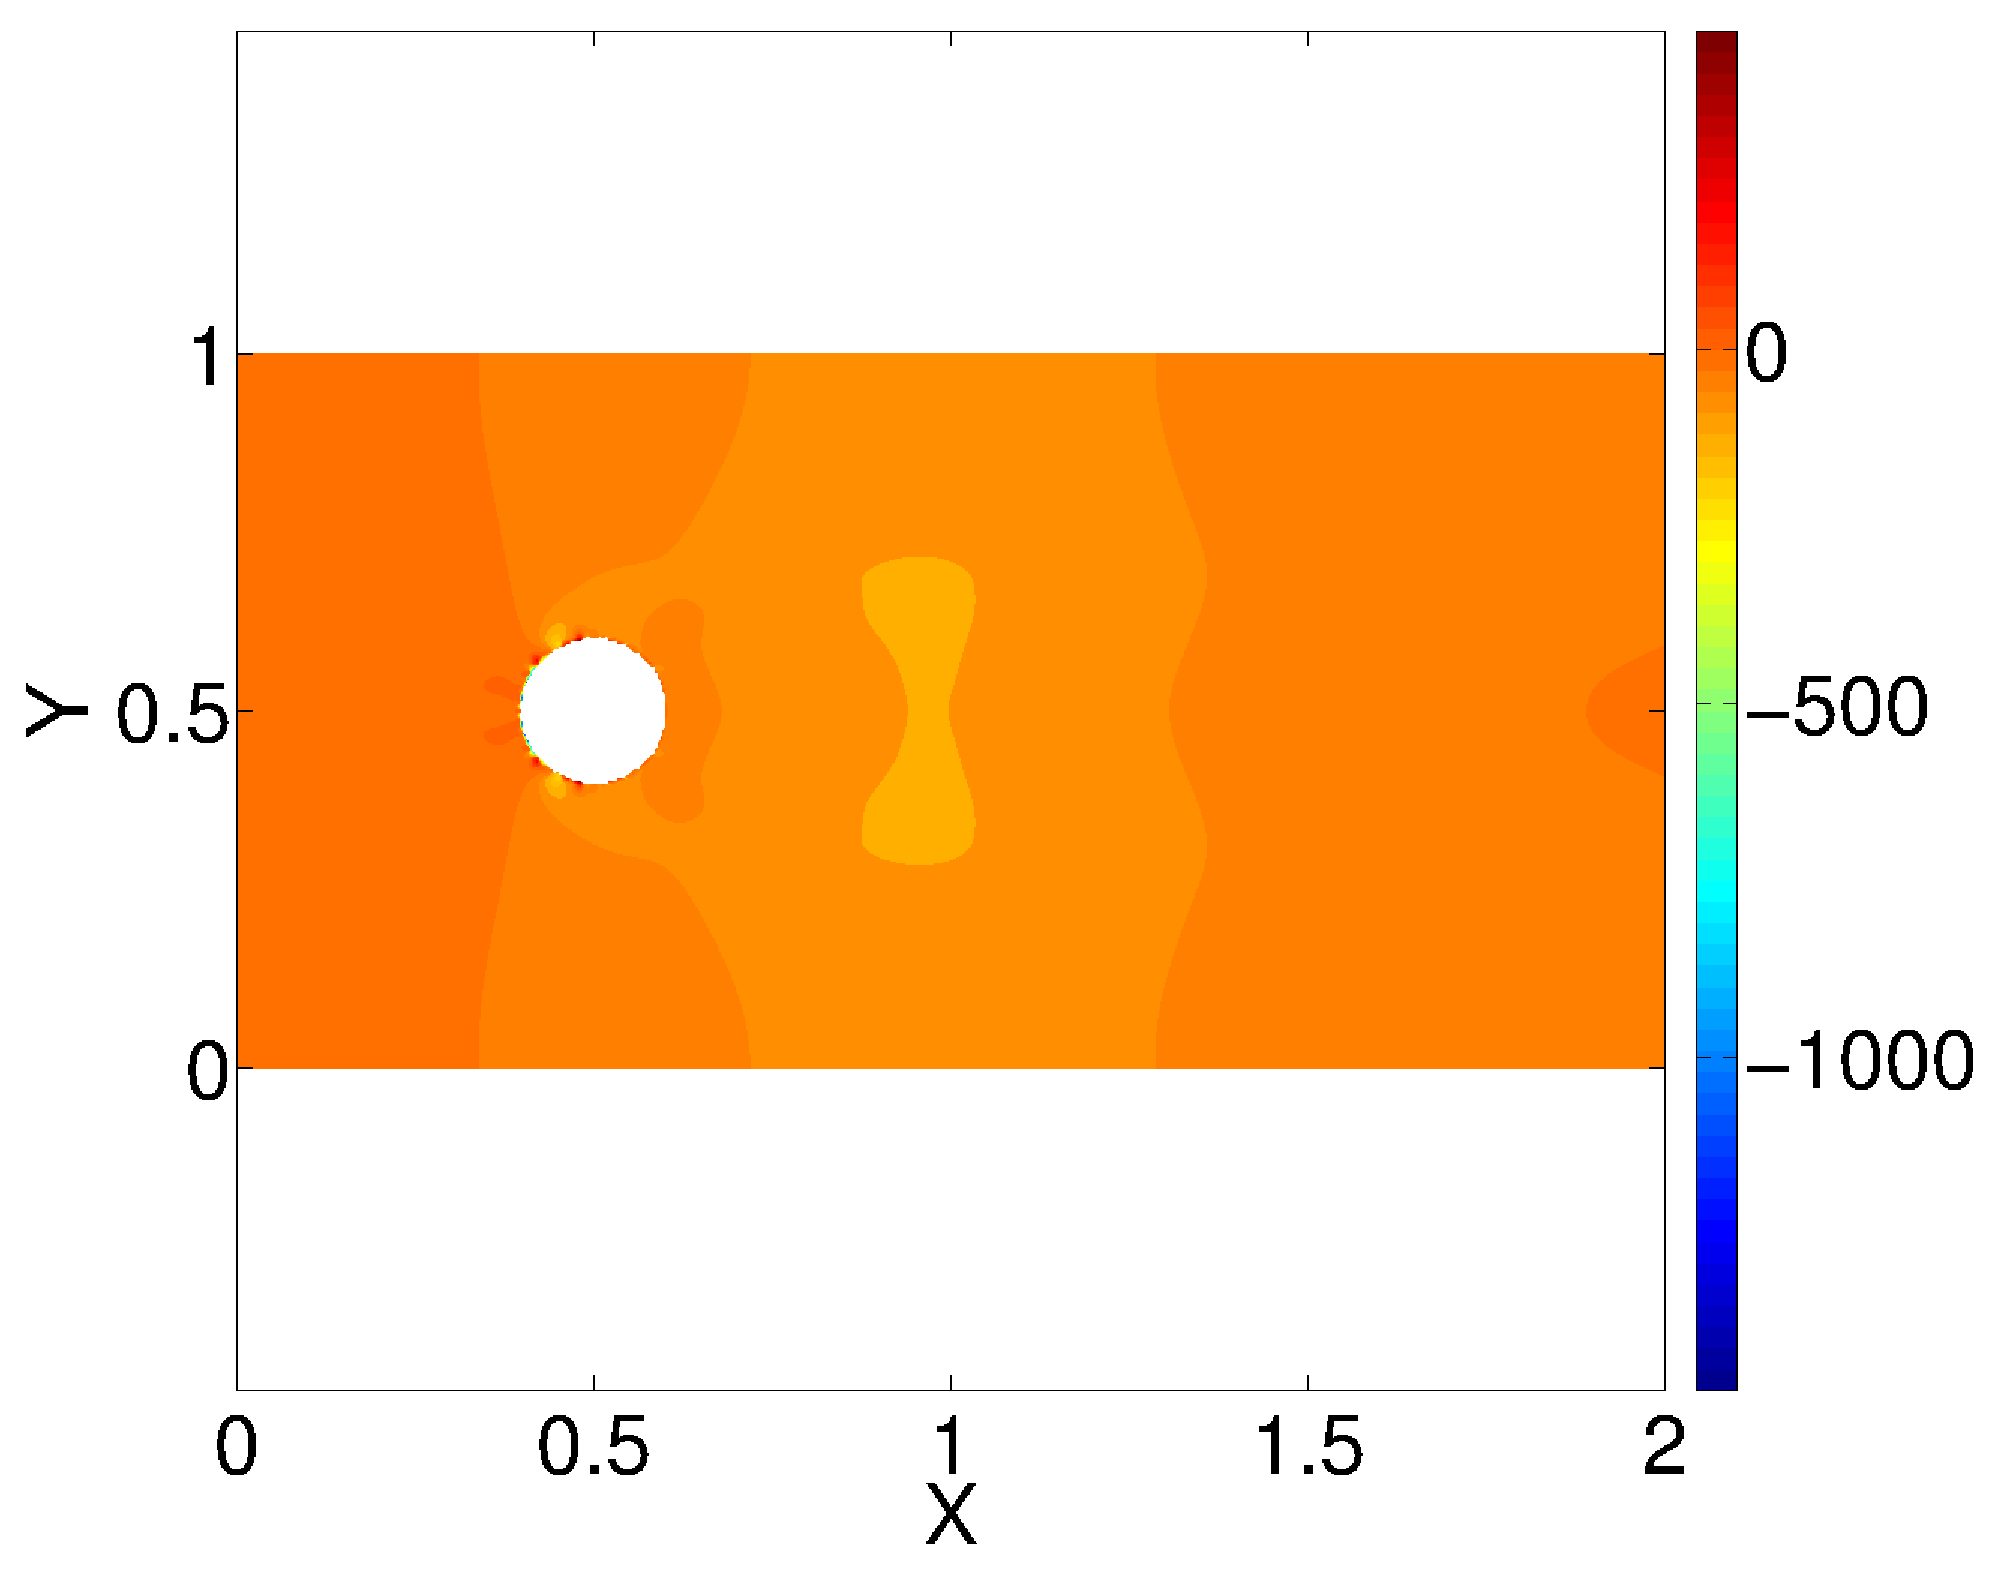
\includegraphics[height=6.0cm]{figure/cylinder/Pp_RE1000.eps}
	}
	\quad
	\subfigure[Complex step result for pressure]
	{
	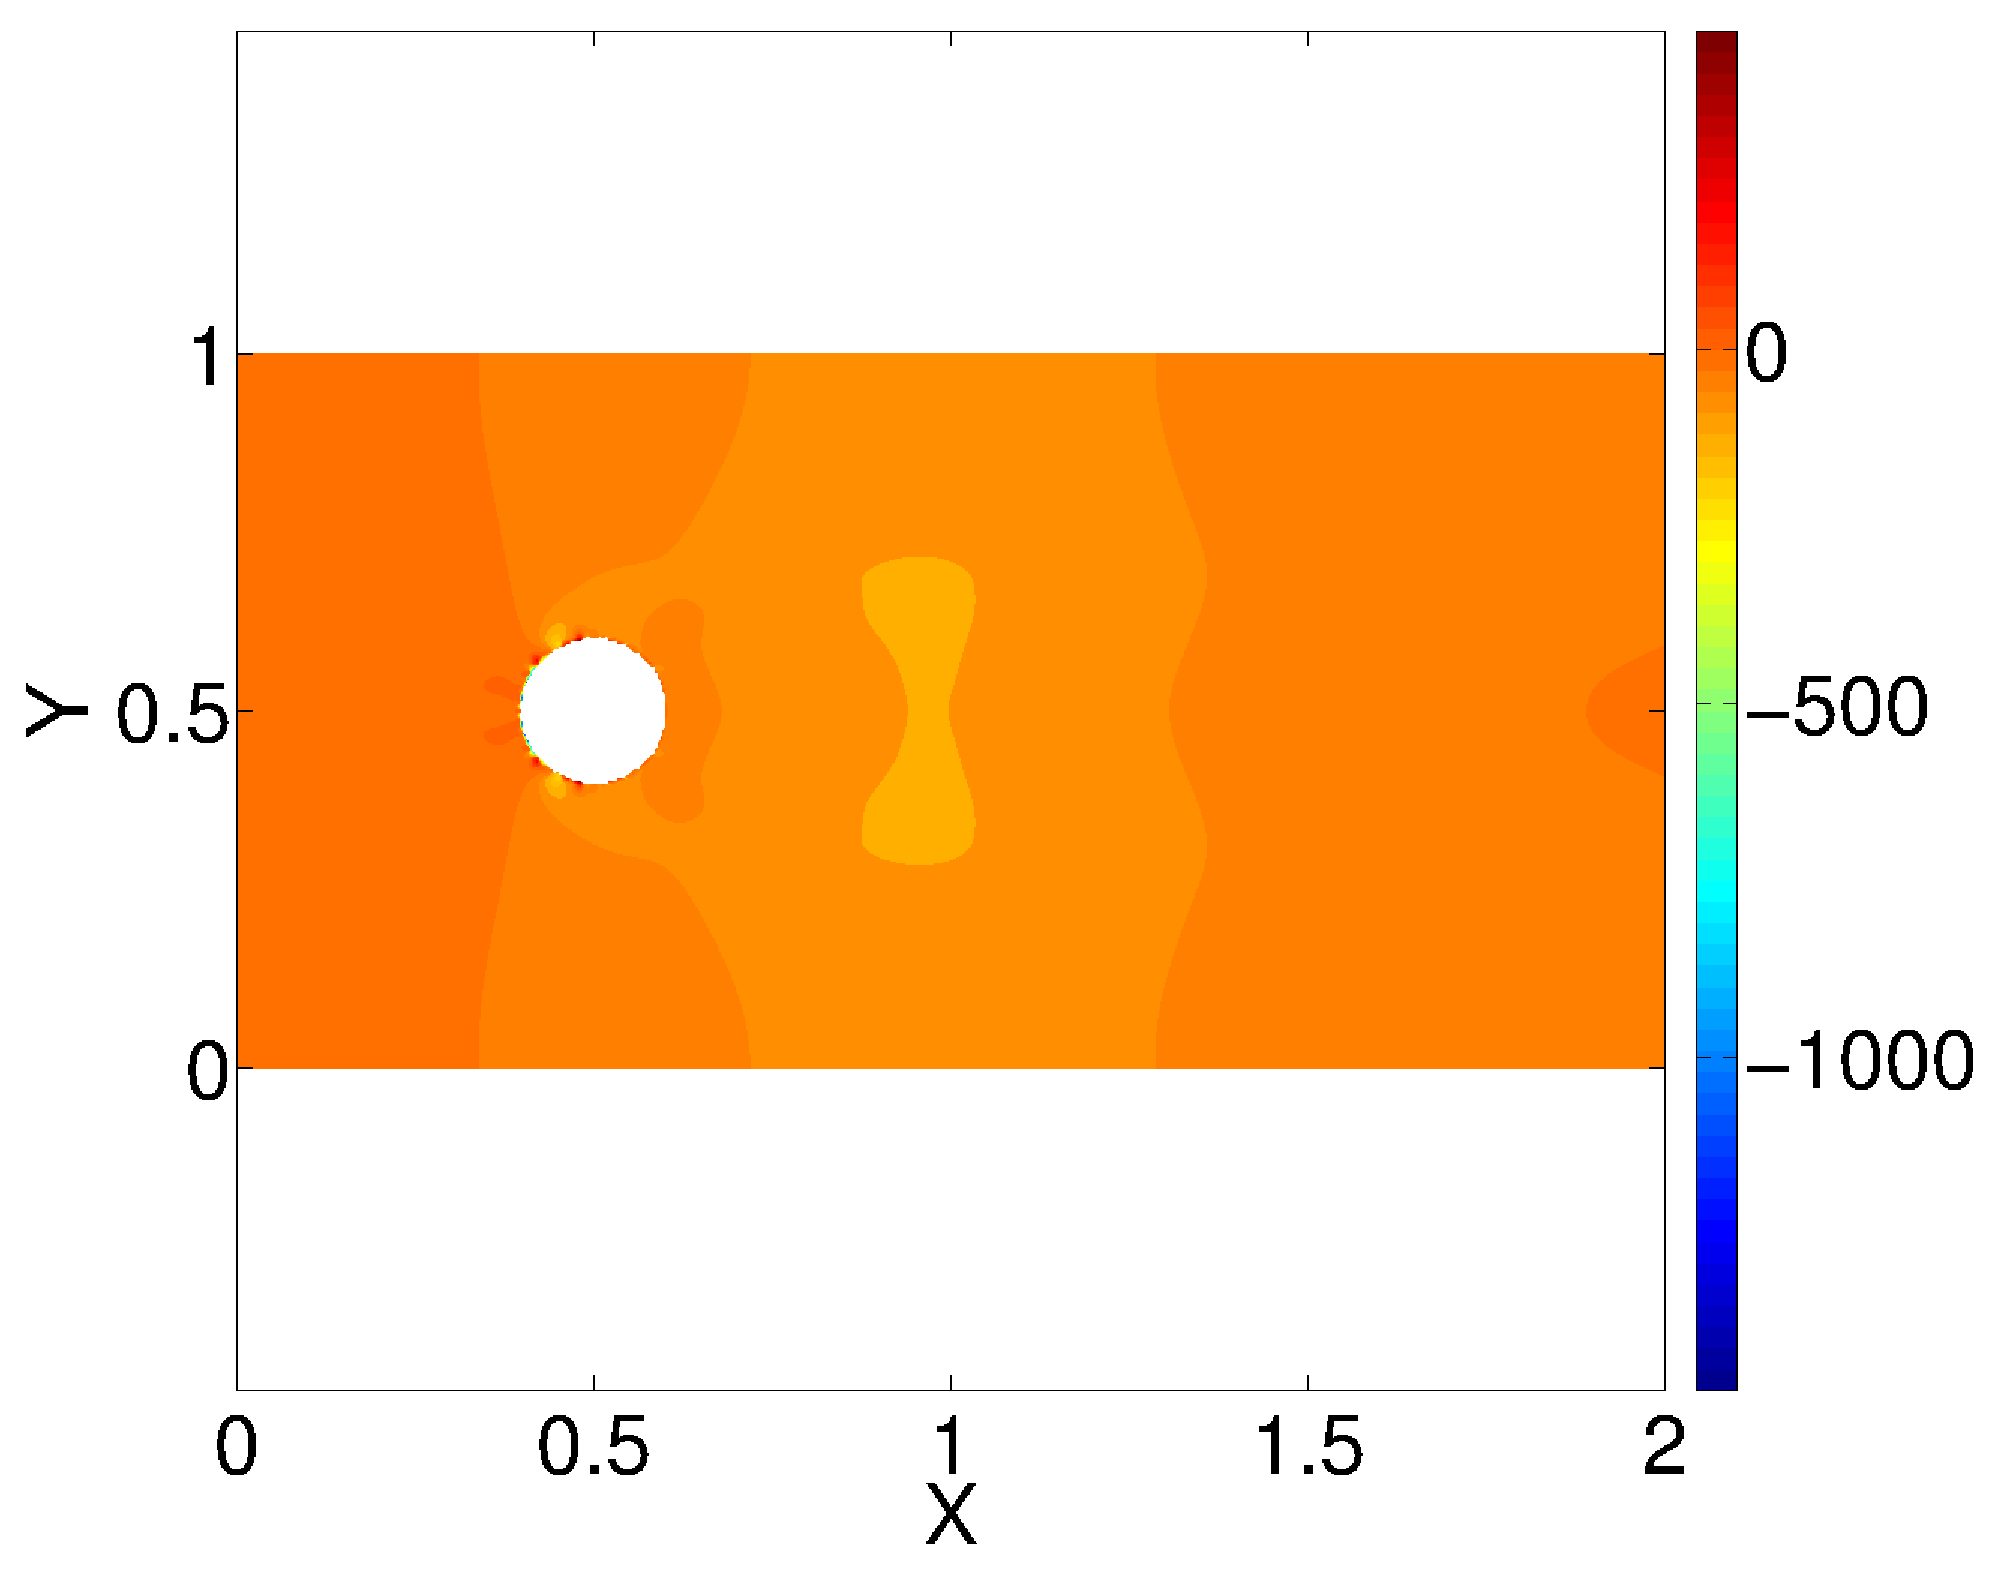
\includegraphics[height=6.0cm]{figure/cylinder/Pp_RE1000.eps}
	}
	\\
	\subfigure[Continuum sensitivity result for u-velocity]
	{
	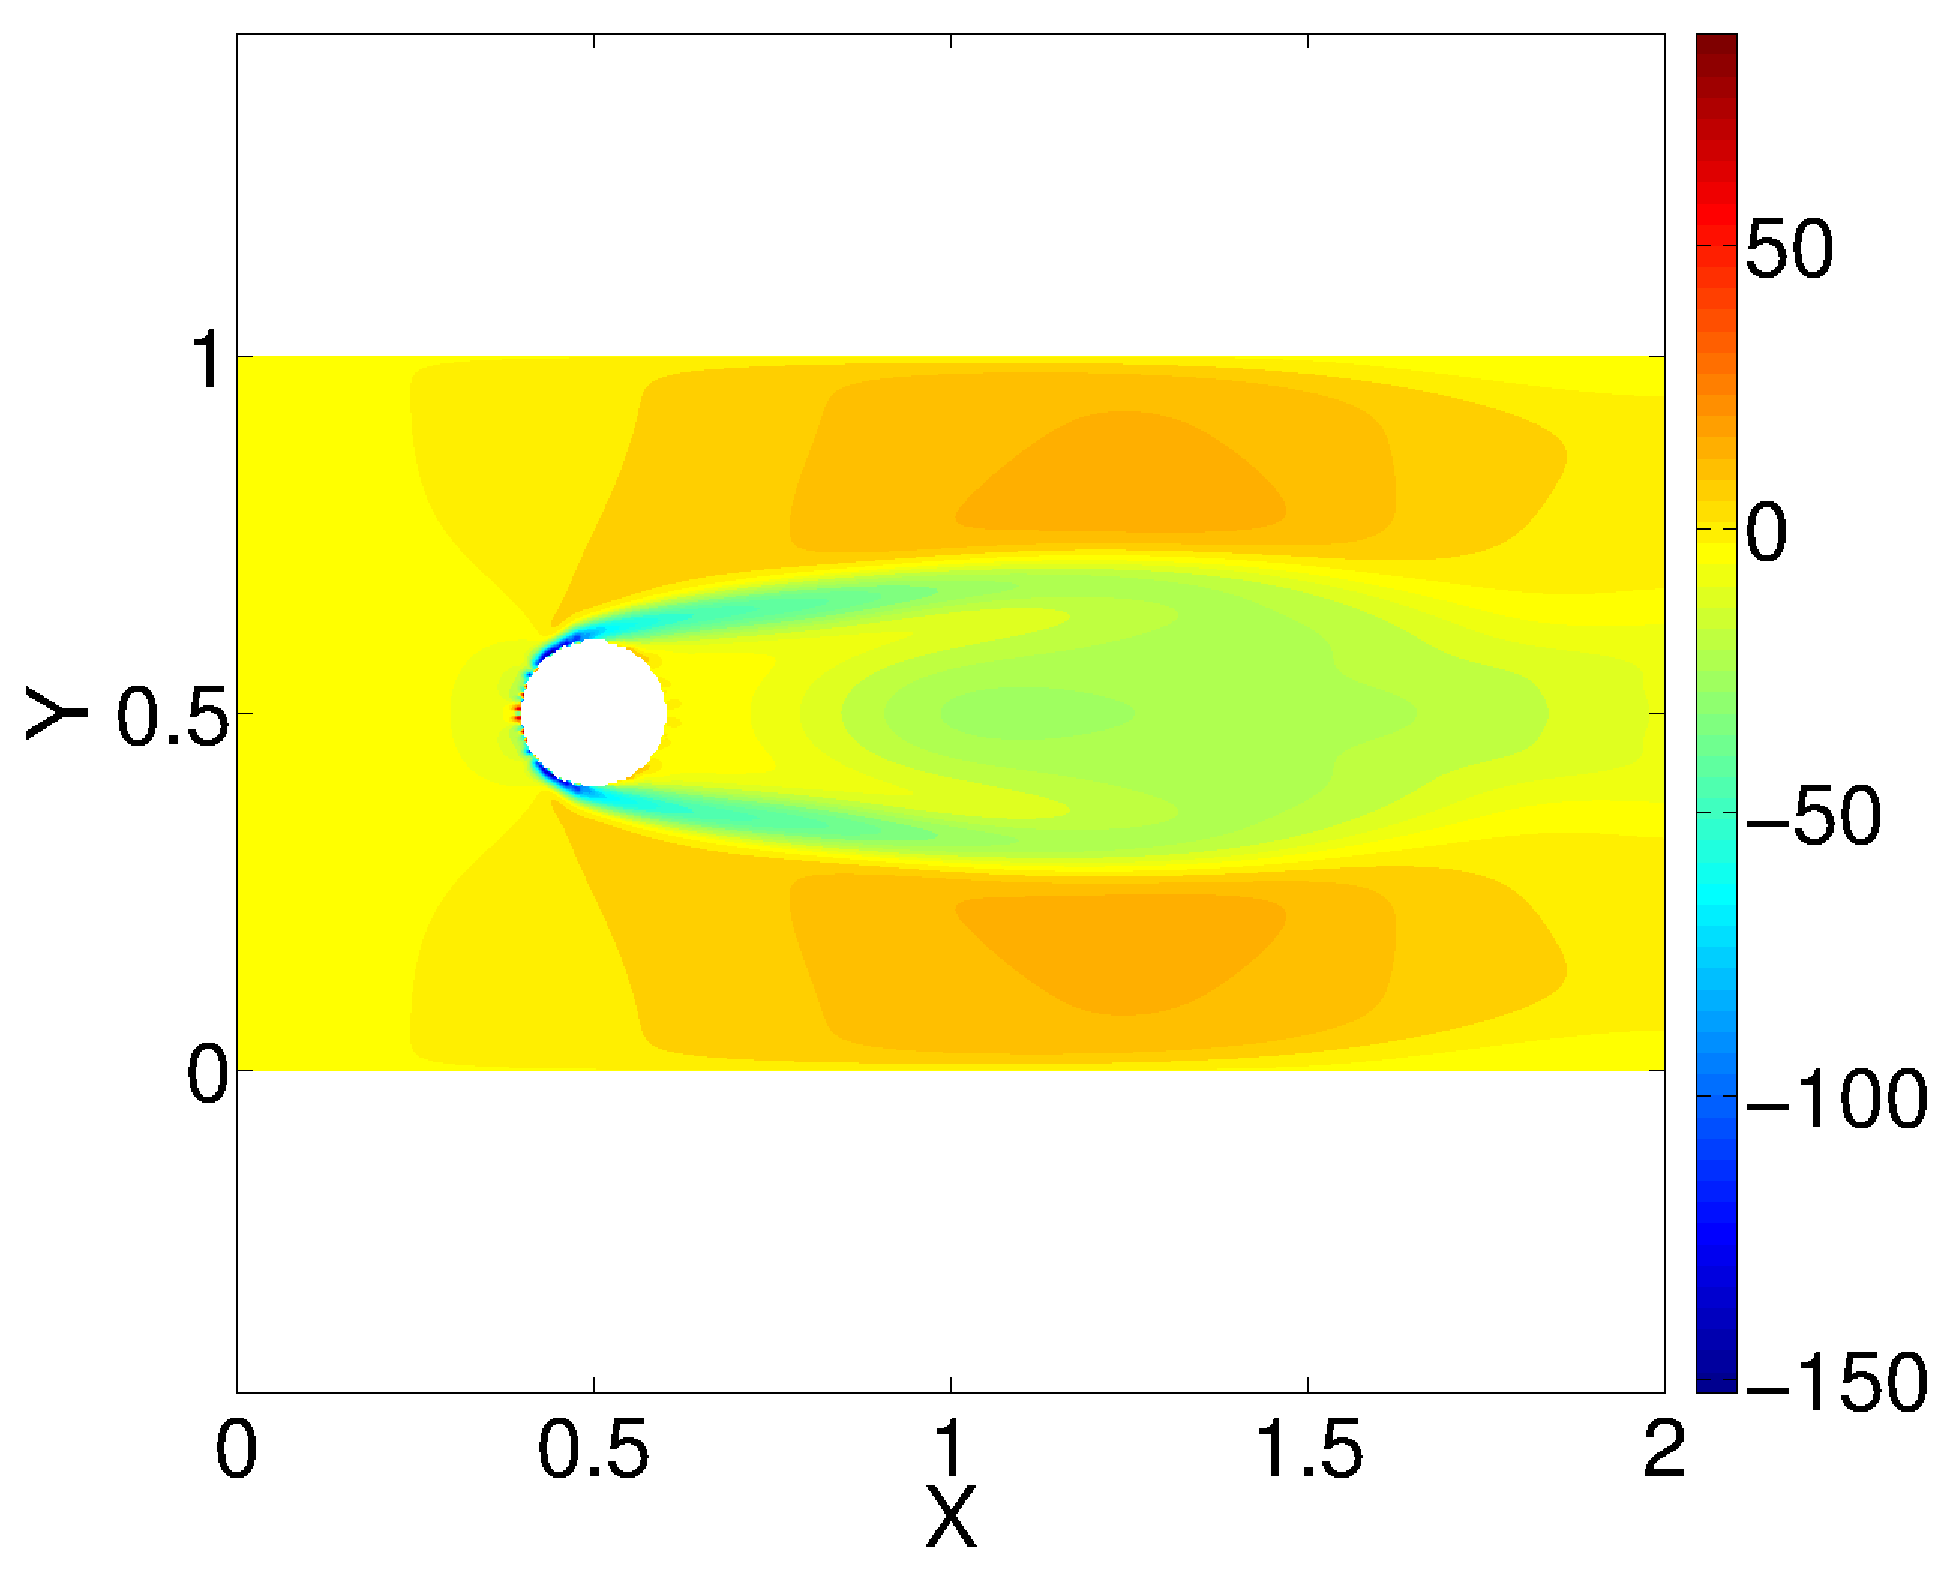
\includegraphics[height=6.0cm]{figure/cylinder/Up_RE1000.eps}
	}
	\quad
	\subfigure[Complex step result for u-velocity]
	{
	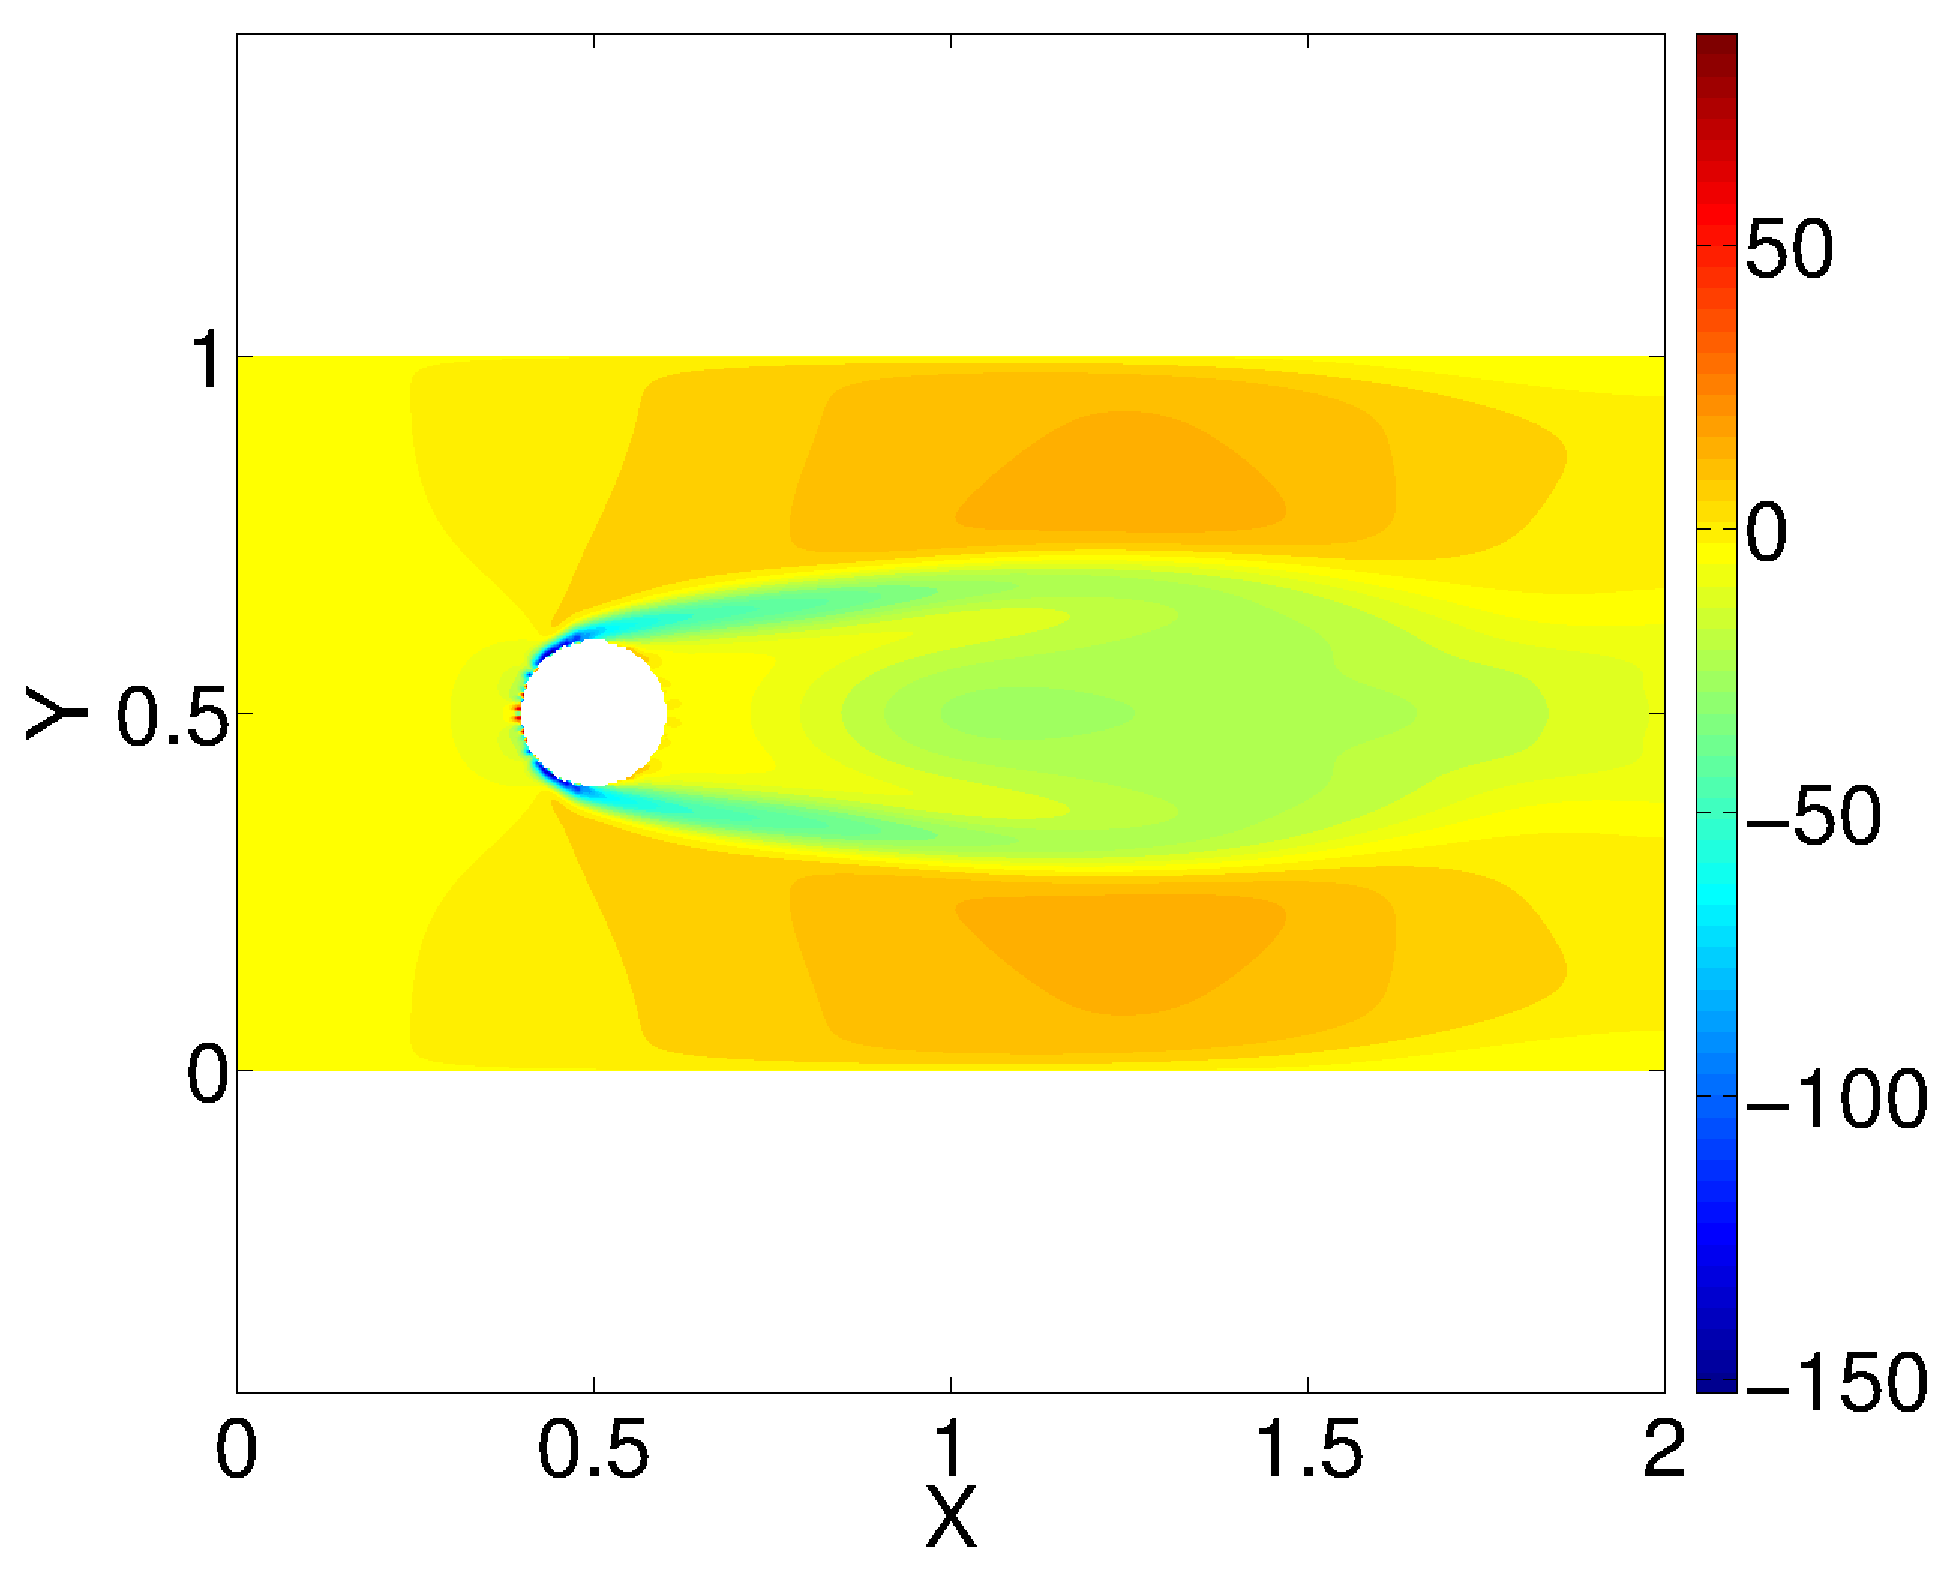
\includegraphics[height=6.0cm]{figure/cylinder/Up_RE1000.eps}
	}
	\\
	\subfigure[Continuum sensitivity result for v-velocity]
	{
	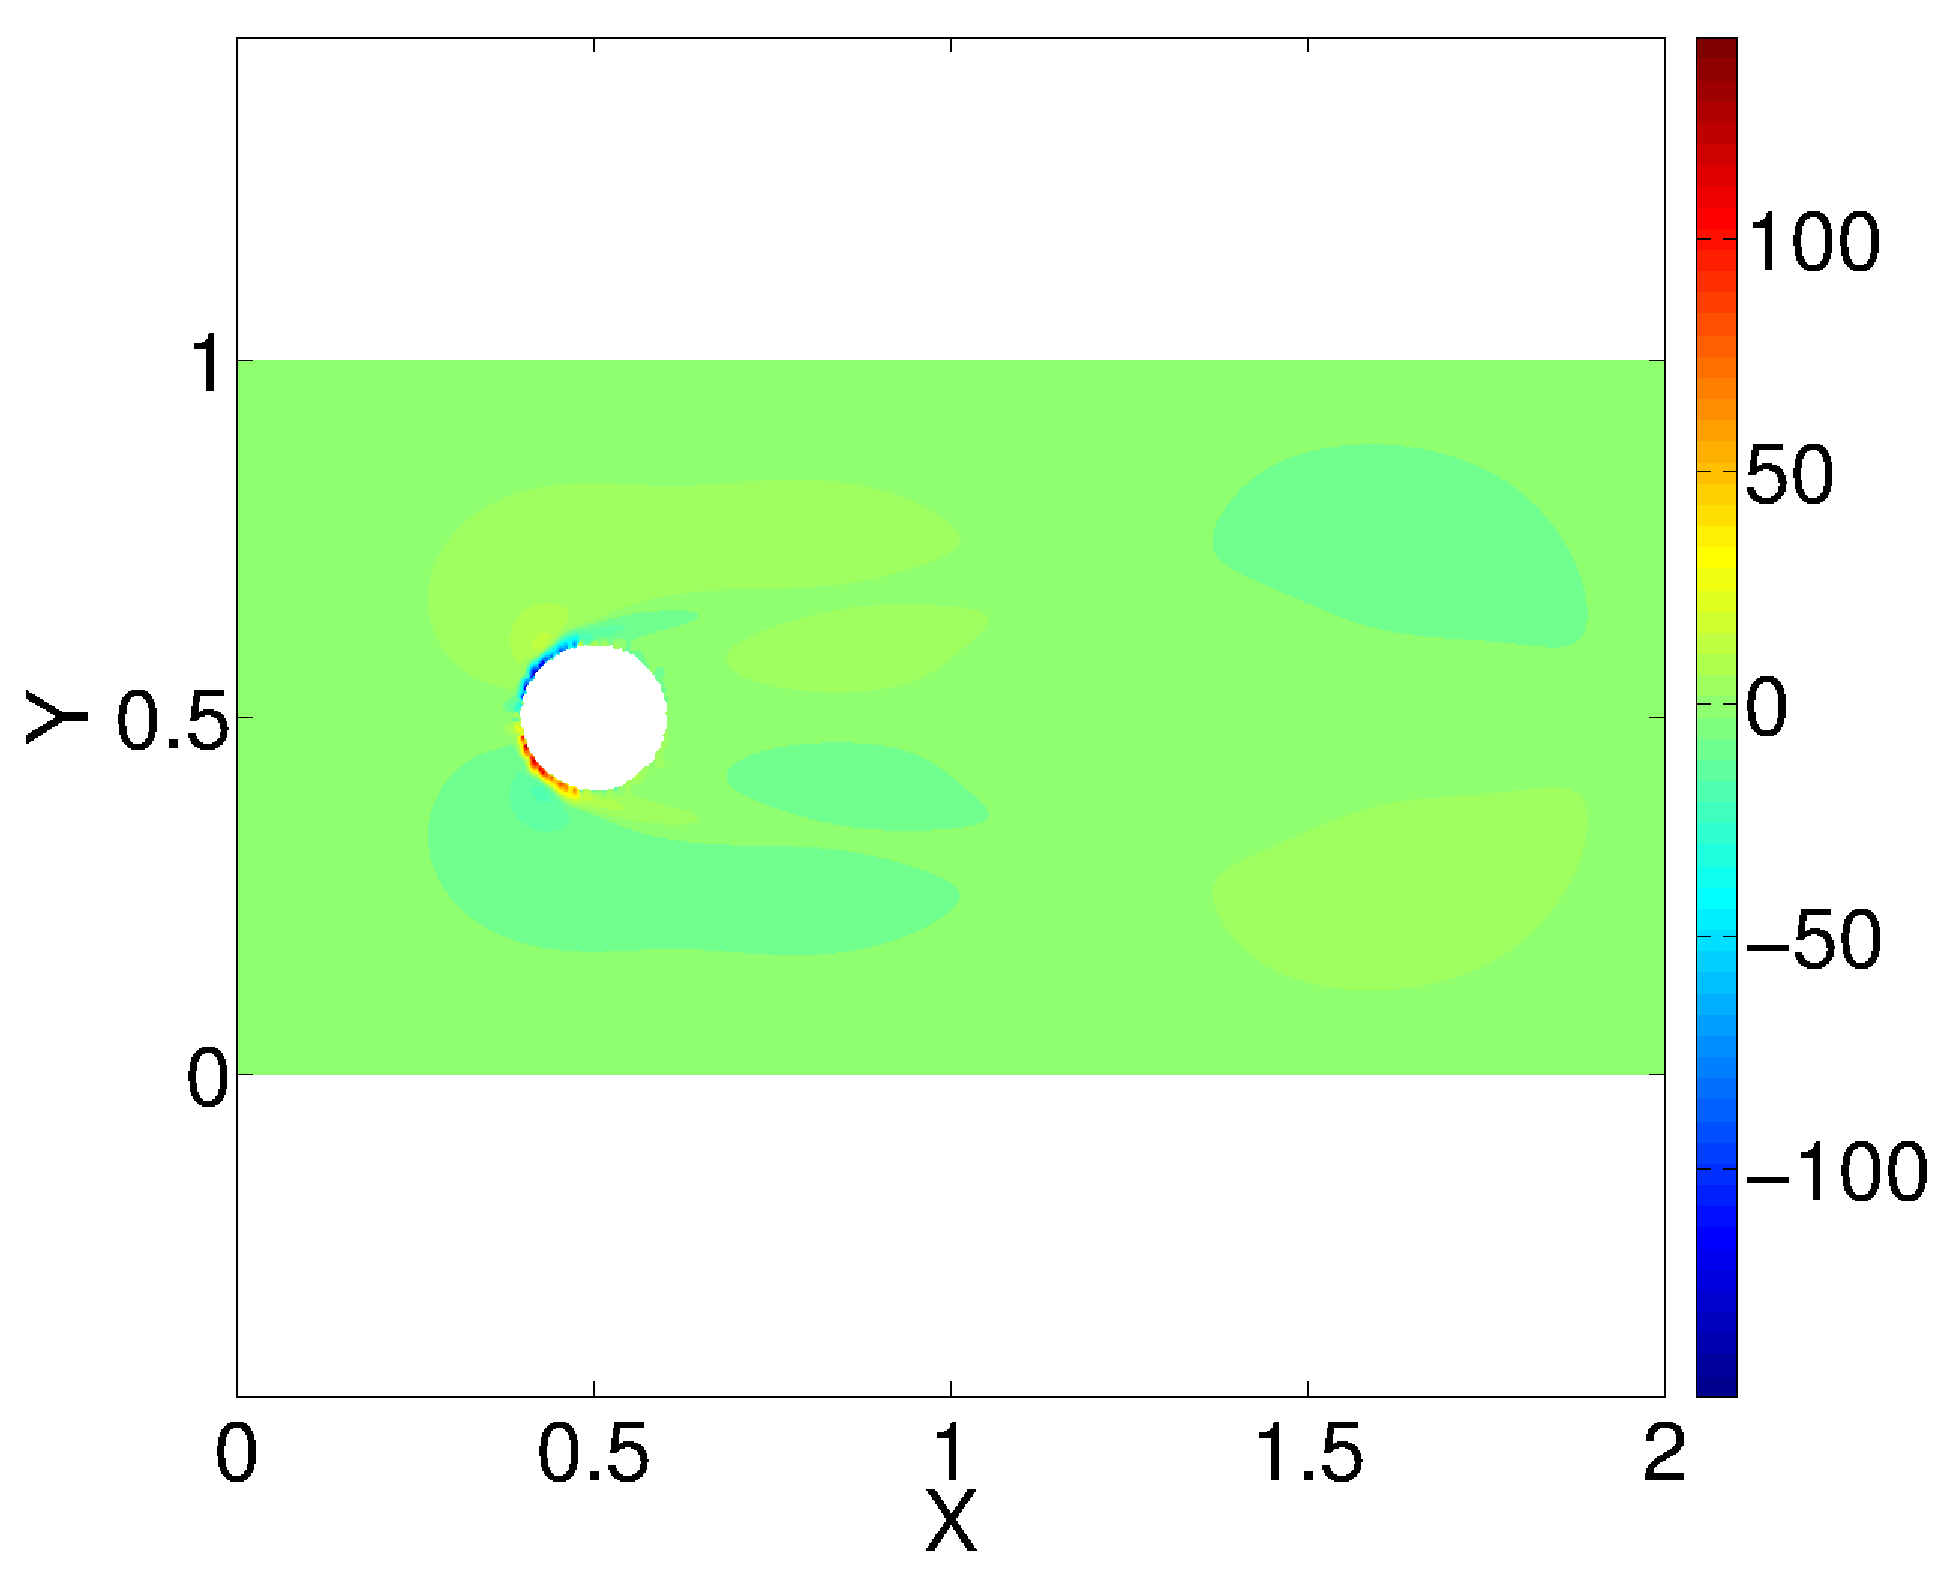
\includegraphics[height=6.0cm]{figure/cylinder/Vp_RE1000.eps}
	}
	\quad
	\subfigure[Complex step result for v-velocity]
	{
	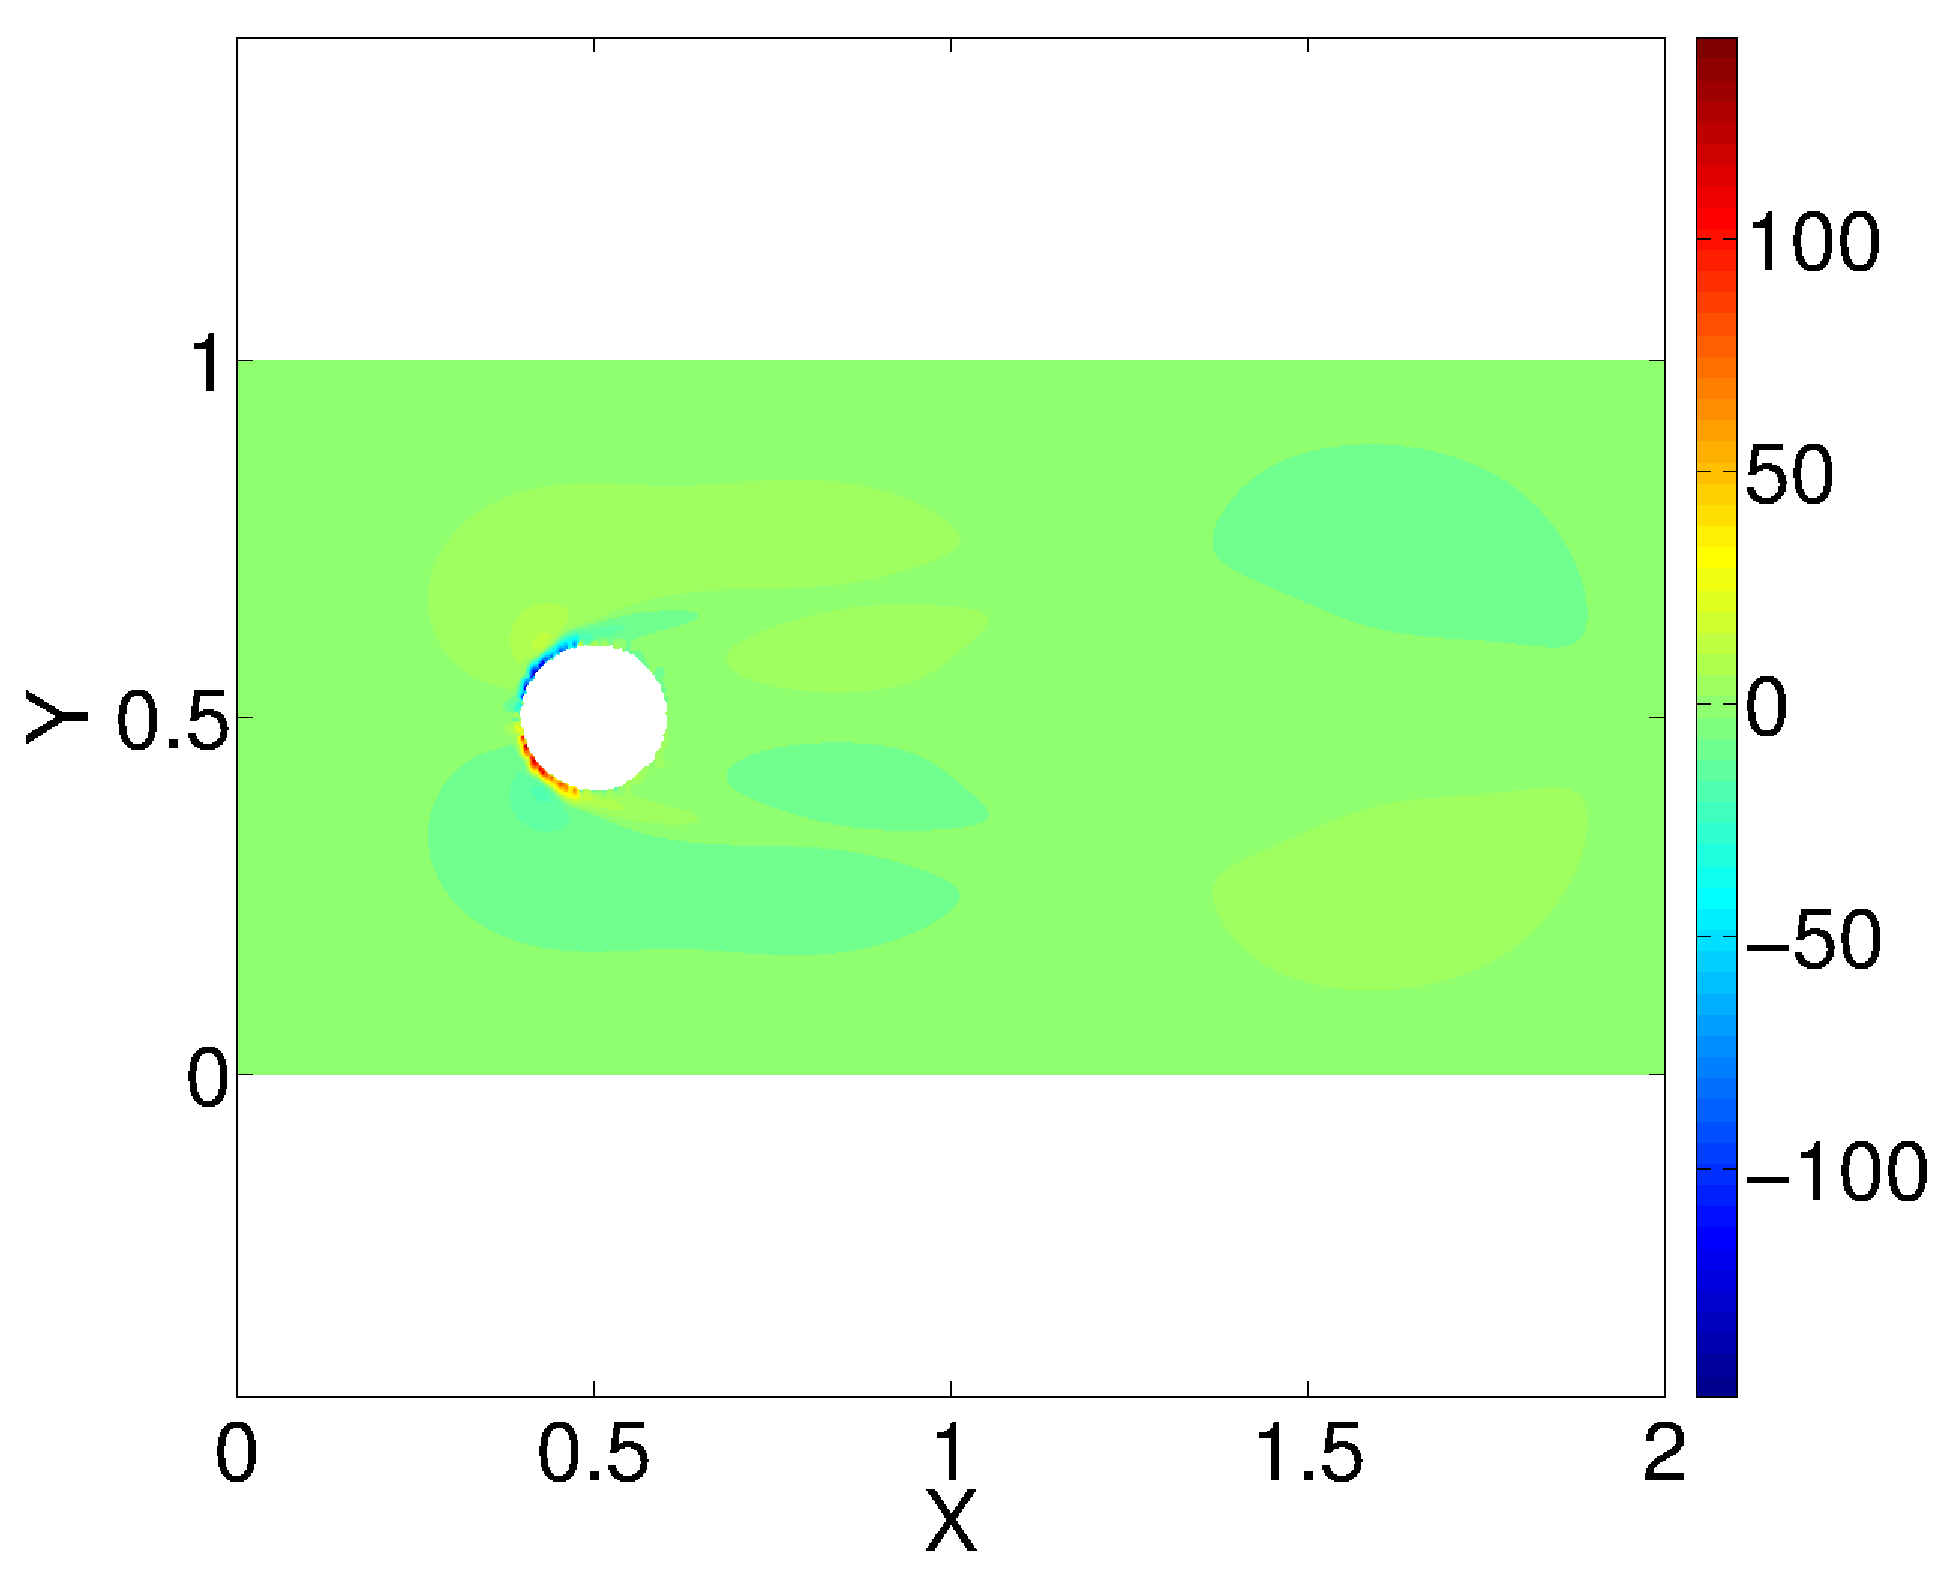
\includegraphics[height=6.0cm]{figure/cylinder/Vp_RE1000.eps}
	}
	\caption{Comparison of sensitivity contours for flow over cylinder, $Re = 1000$.}
	\label{fig:cylinderSensitivityContourRE1000}
\end{figure}
%

For a better comparison between the sensitivity results of Continuum Sensitivity Analysis (CSA) and Complex Step (CS) methods, we looked at different locations in the computational domain. These locations are indicated in Figure \ref{fig:cylinderSampleLocations}.

%
\begin{figure}[H]
	\centering
	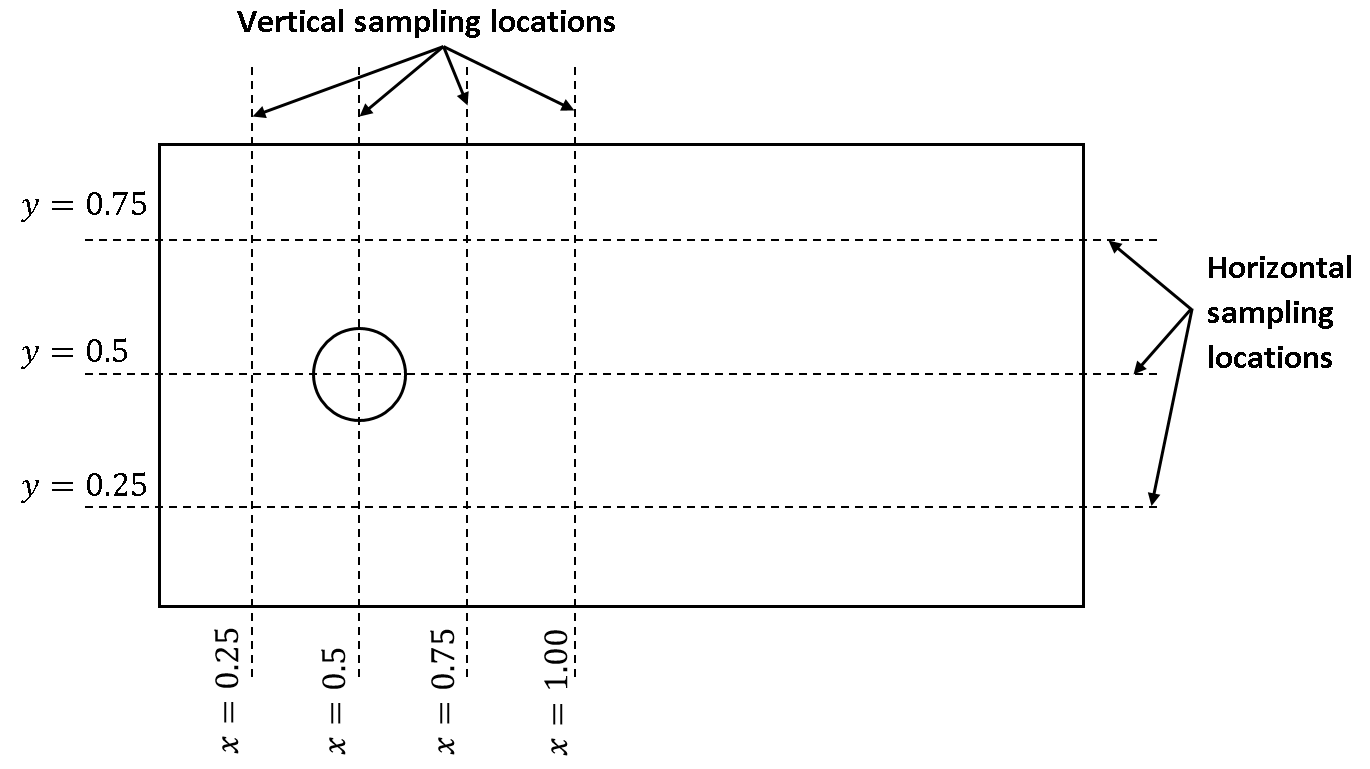
\includegraphics[height=6.0cm]{figure/cylinder/sampling_location.png}
	\caption{Sampling locations for the sensitivities}
	\label{fig:cylinderSampleLocations}
\end{figure}
%

We compared the sensitivity of u-velocity and pressure at the sample locations for different Reynolds number values. As shown in Figures \ref{fig:cylinderPressureSensitivity} and \ref{fig:cylinderVelocitySensitivity}, the continuum sensitivity and complex step results agree well with each other.

%
\begin{figure}[H]
	\centering
	\subfigure[y = 0.25, Re = 100]
	{
	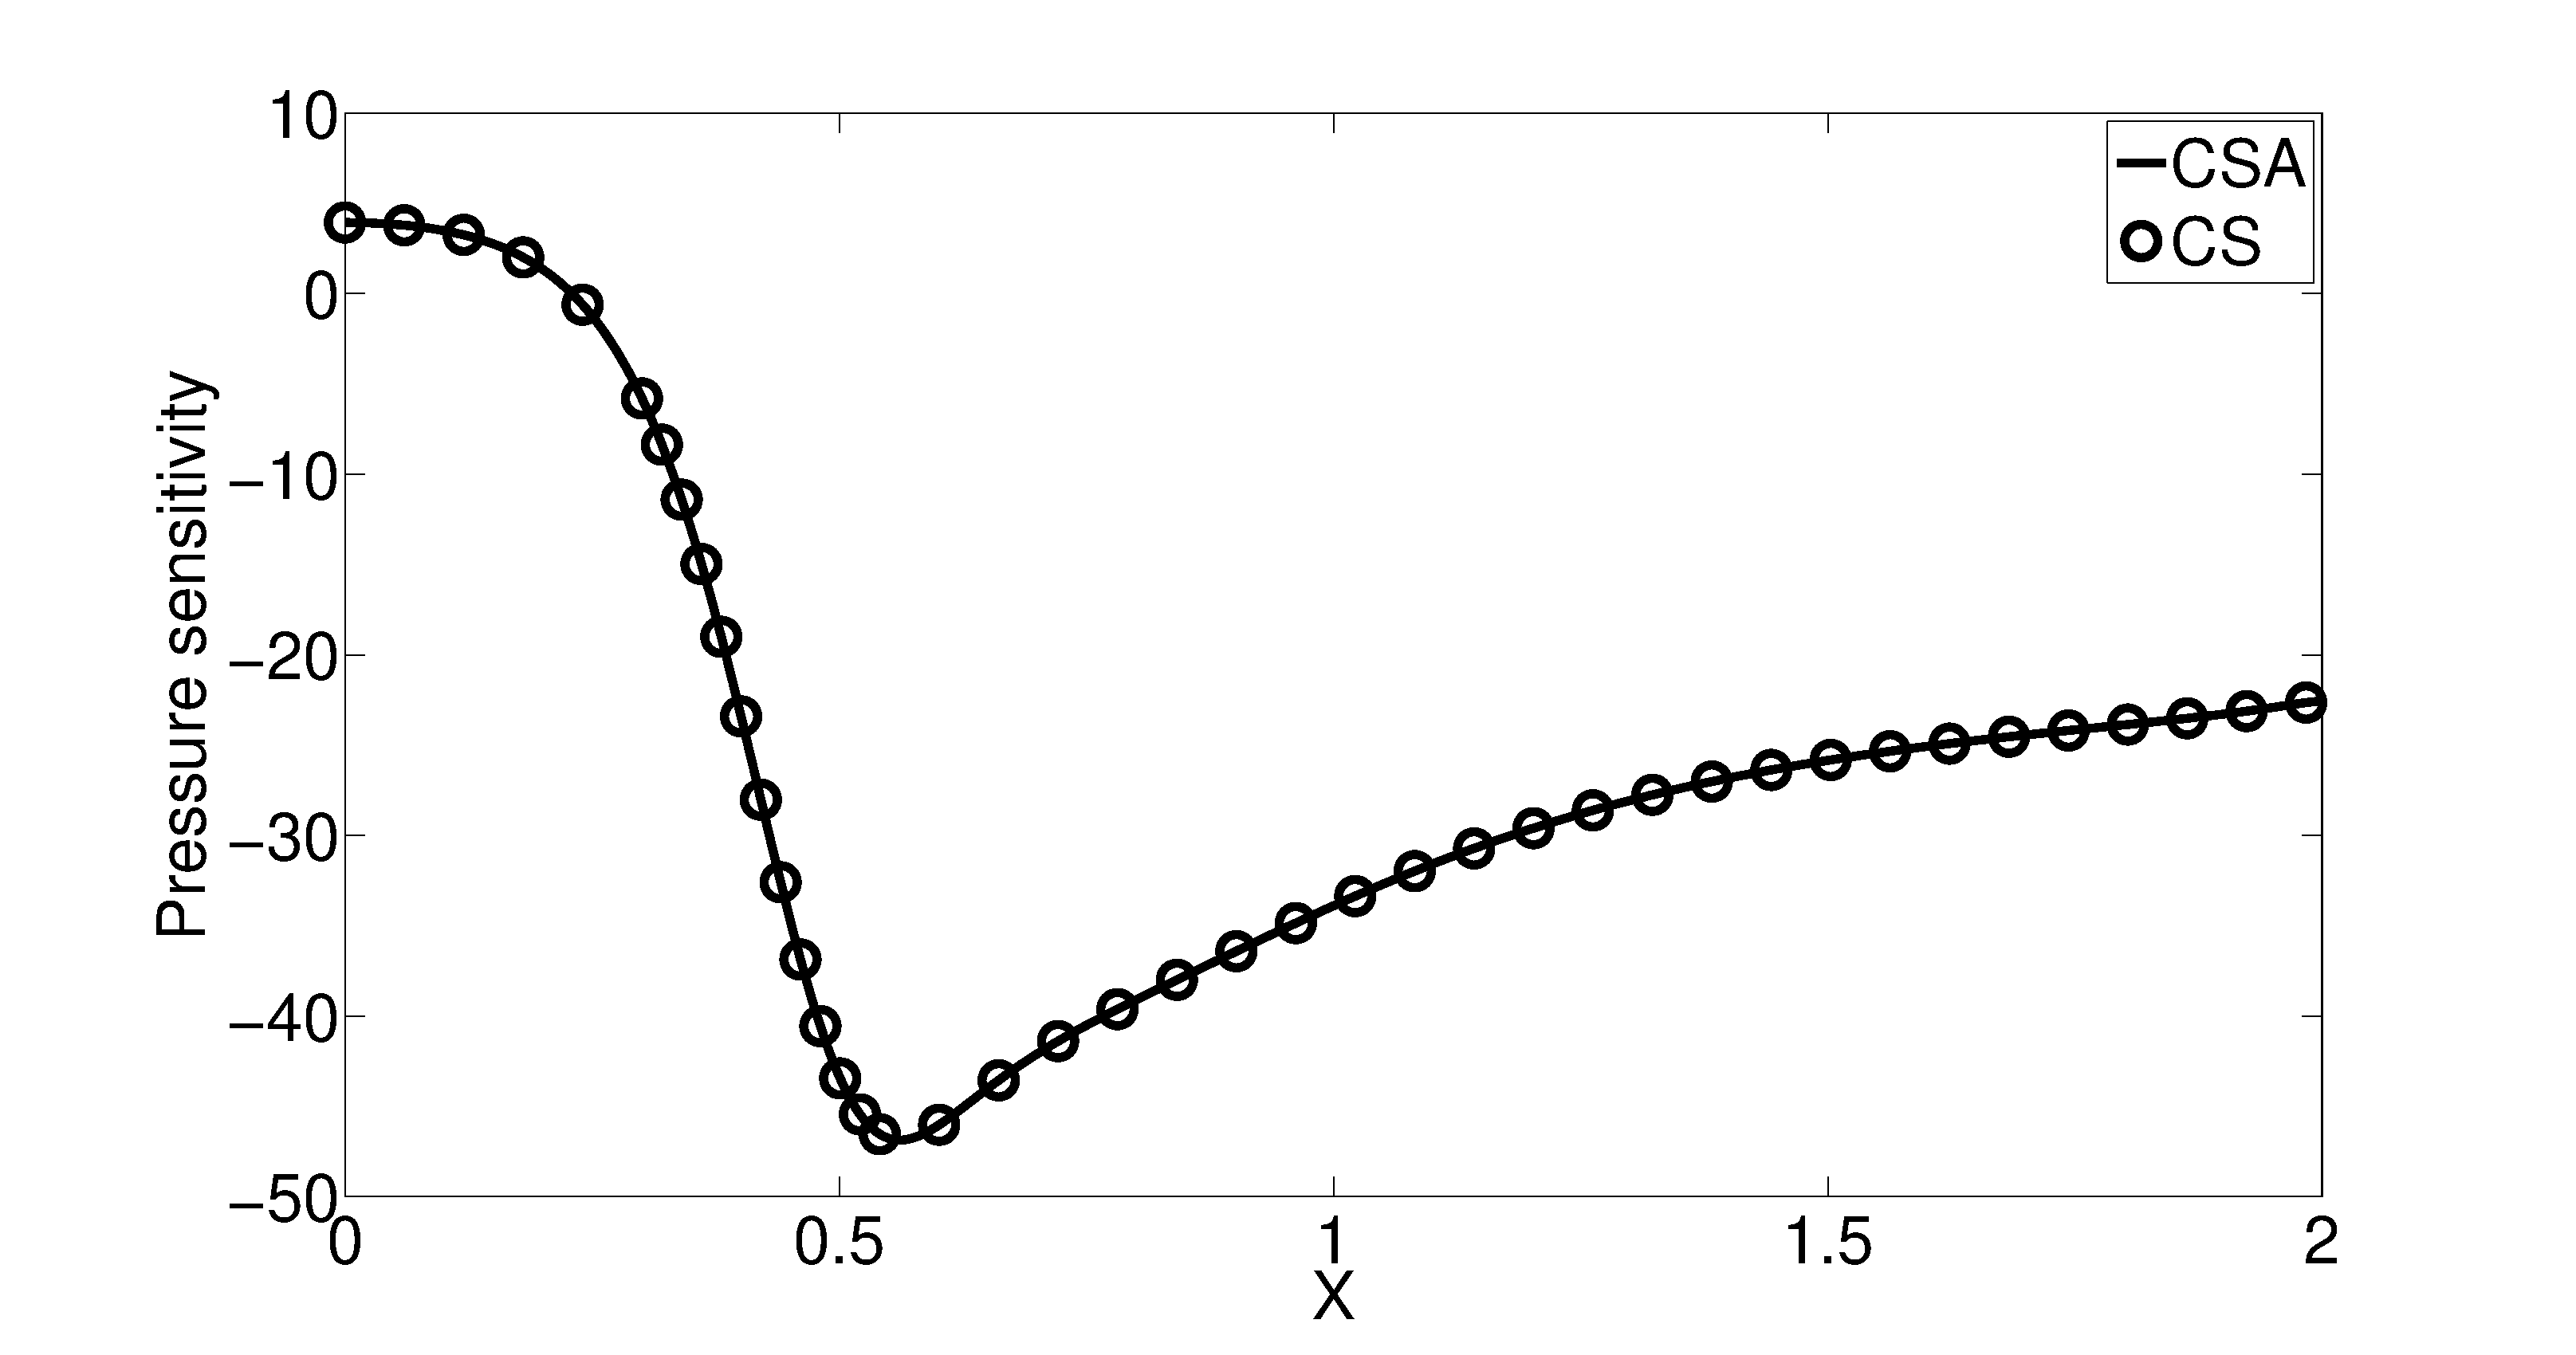
\includegraphics[height=4.0cm]{figure/cylinder/Pp025_RE100.eps}
	}
	\quad
	\subfigure[y = 0.25, Re = 1000]
	{
	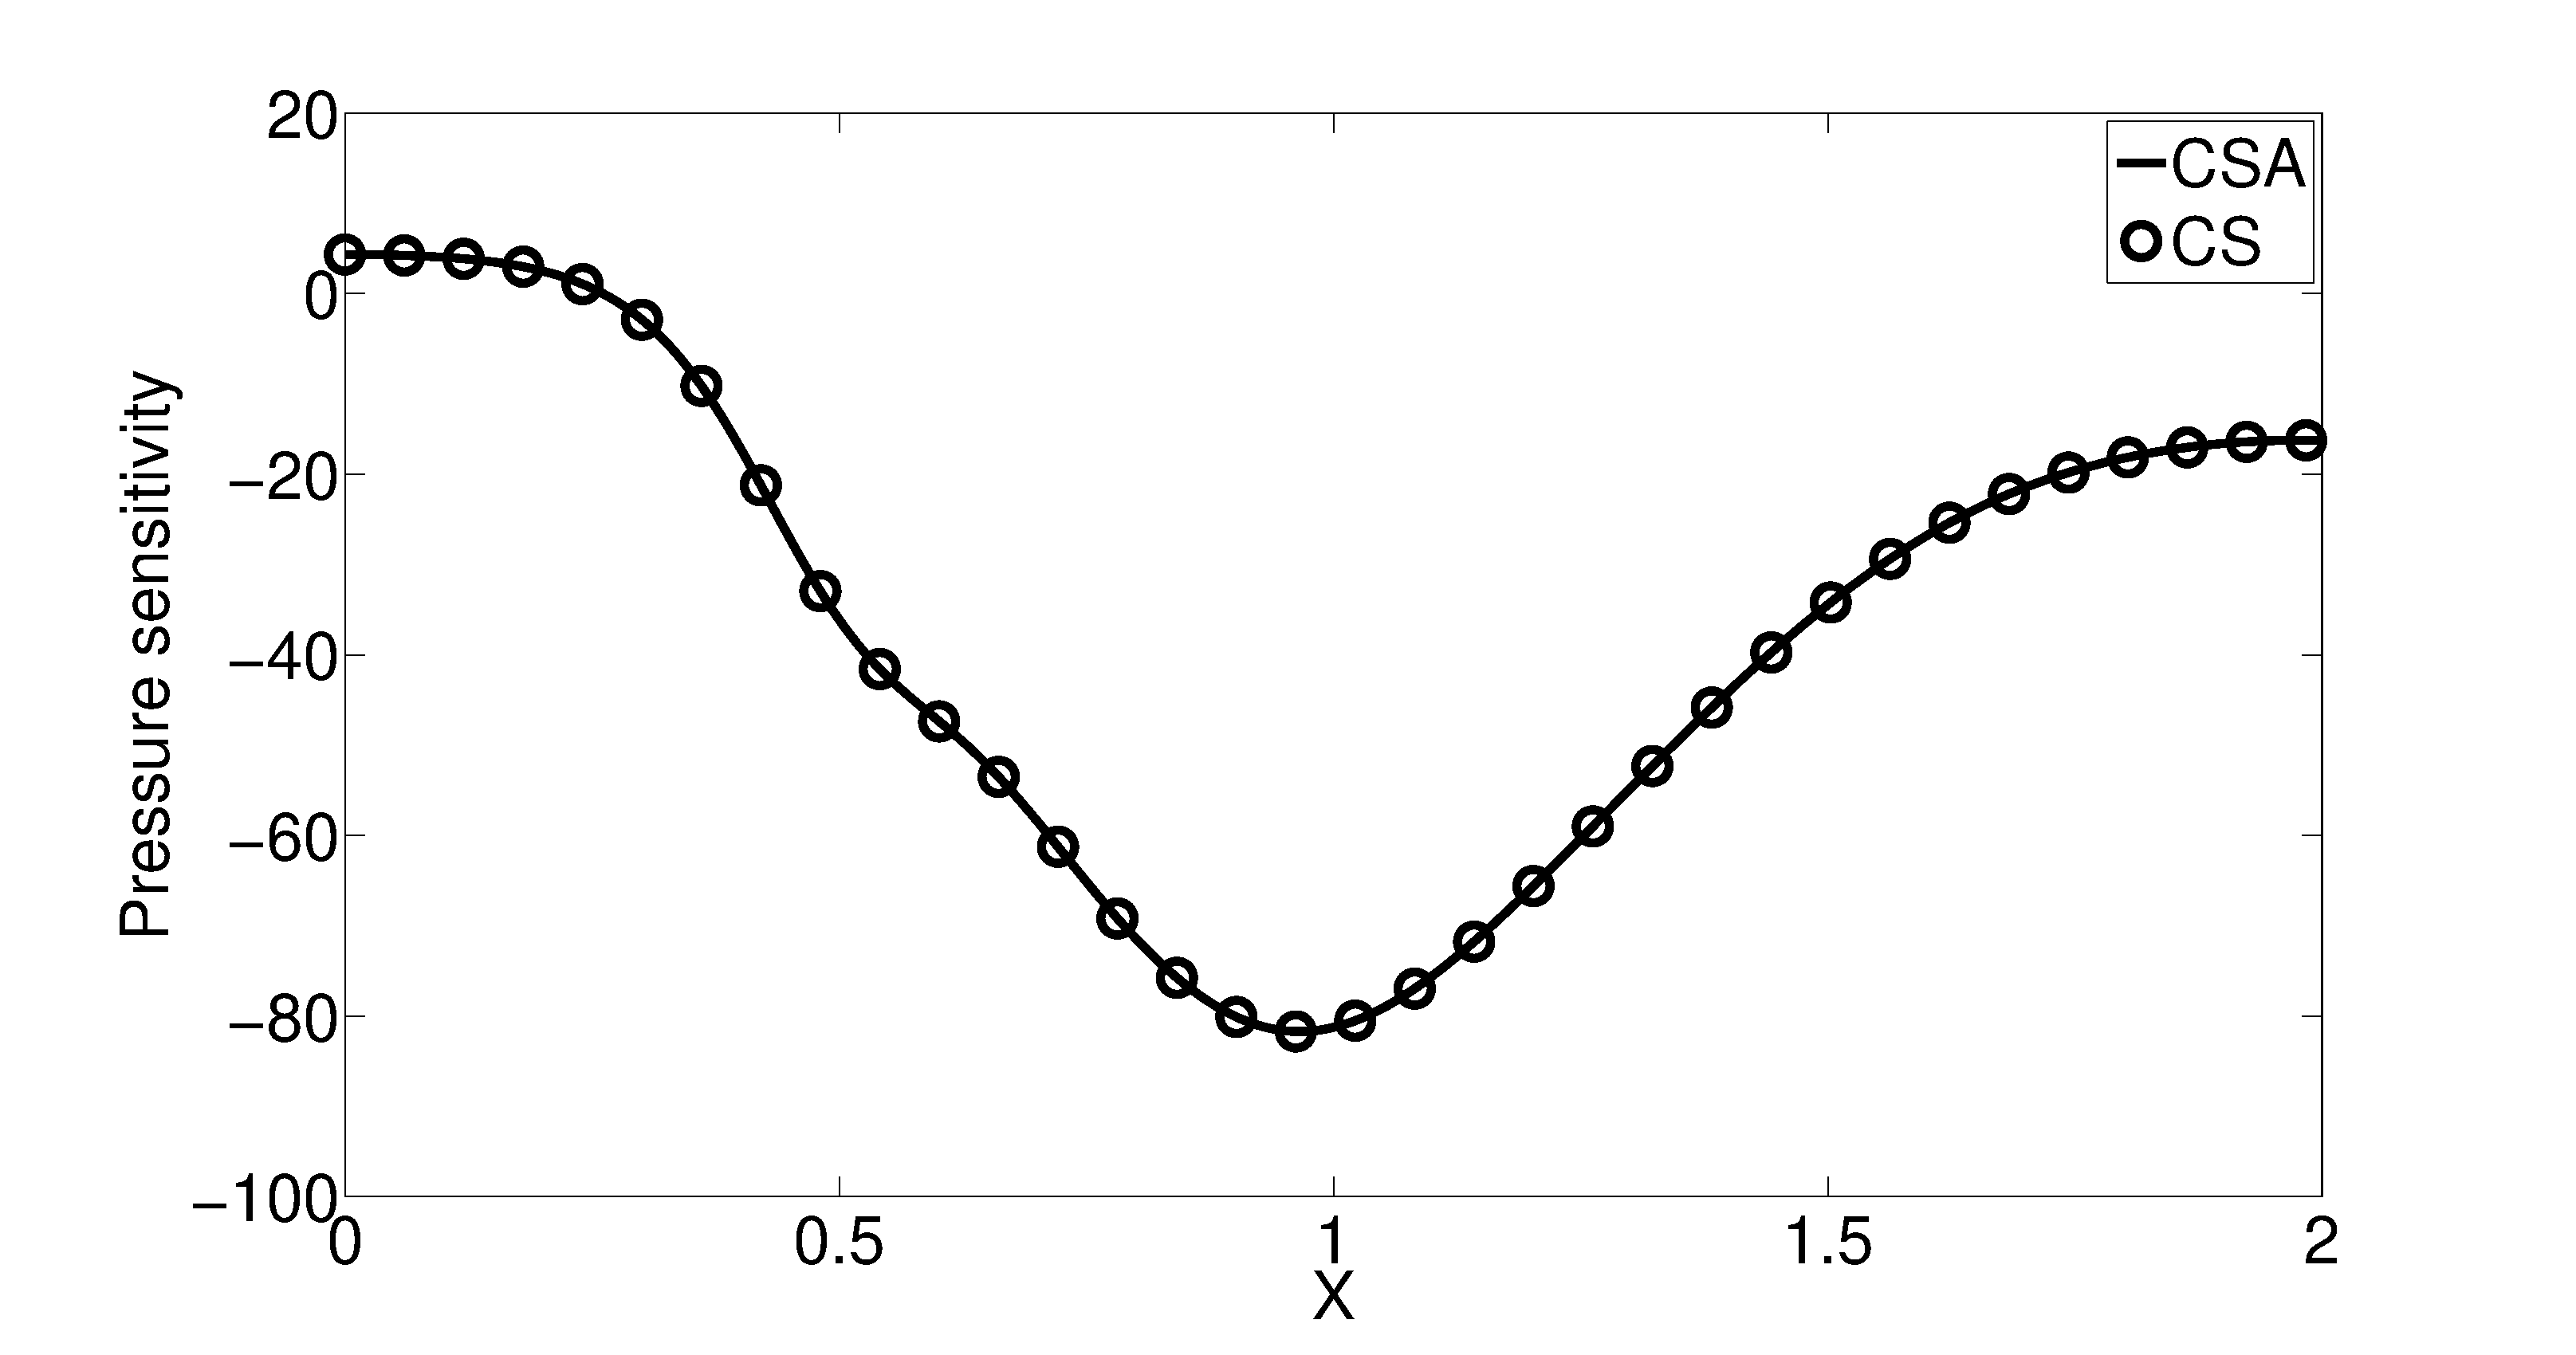
\includegraphics[height=4.0cm]{figure/cylinder/Pp025_RE1000.eps}
	}
	\\
	\subfigure[y = 0.5, Re = 100]
	{
	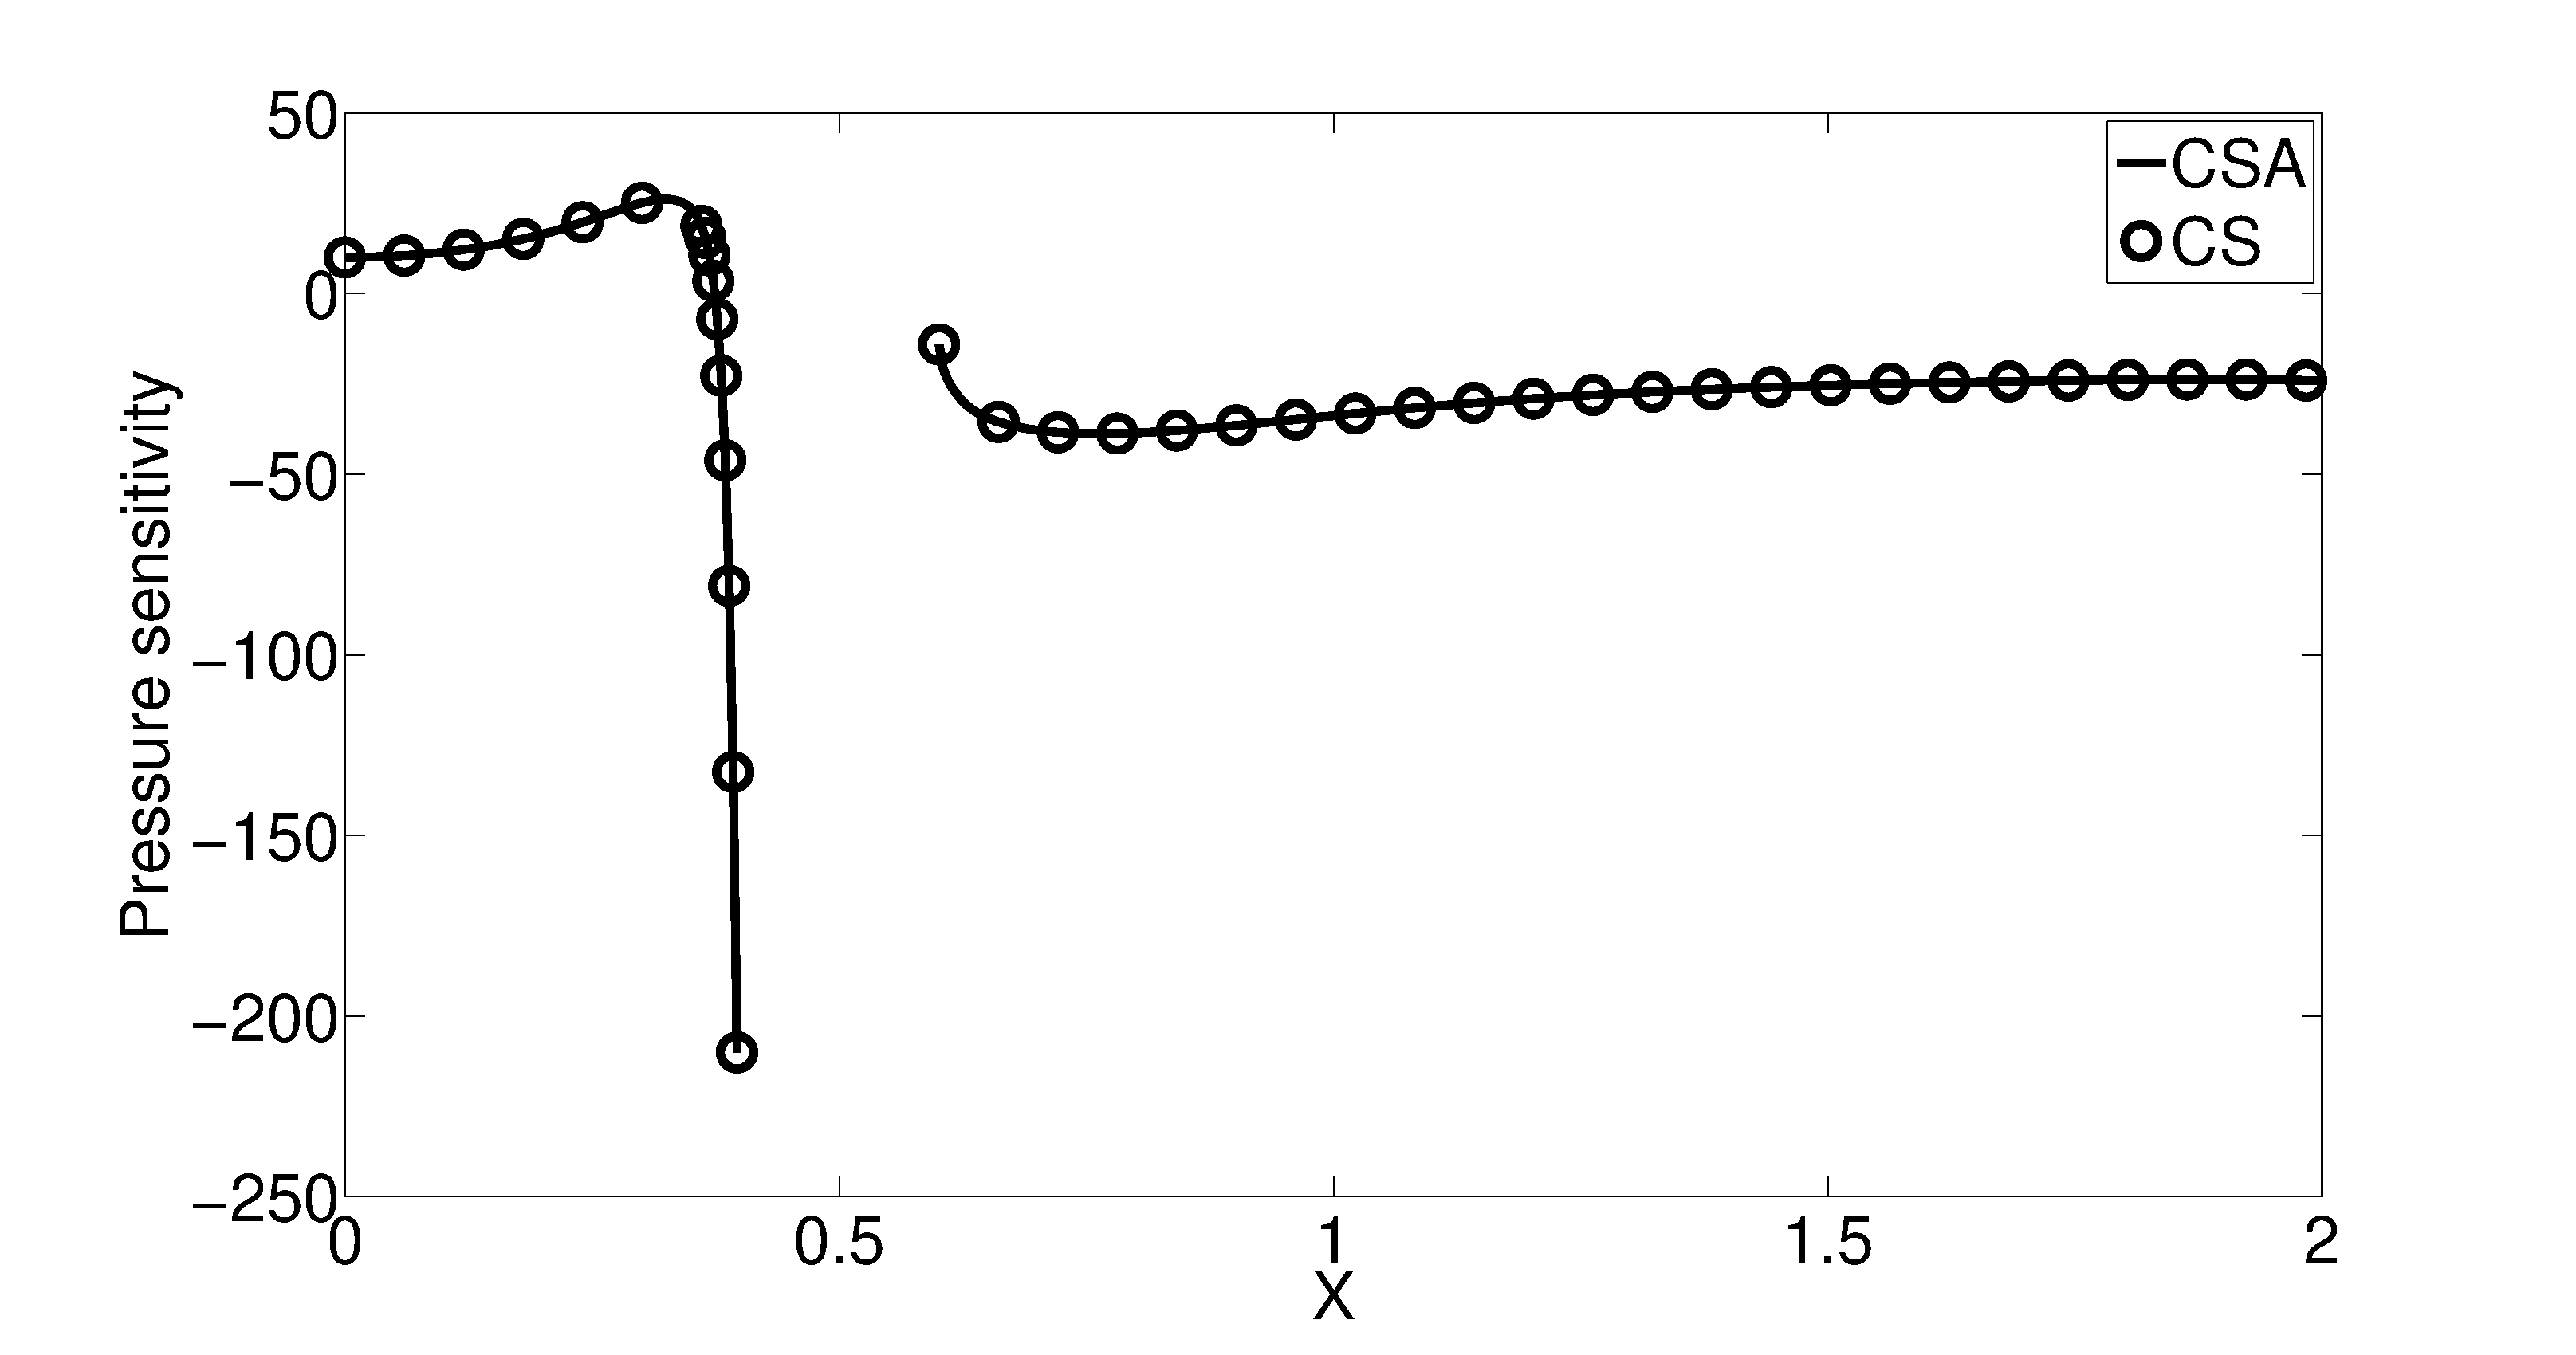
\includegraphics[height=4.0cm]{figure/cylinder/Pp050_RE100.eps}
	}
	\quad
	\subfigure[y = 0.5, Re = 1000]
	{
	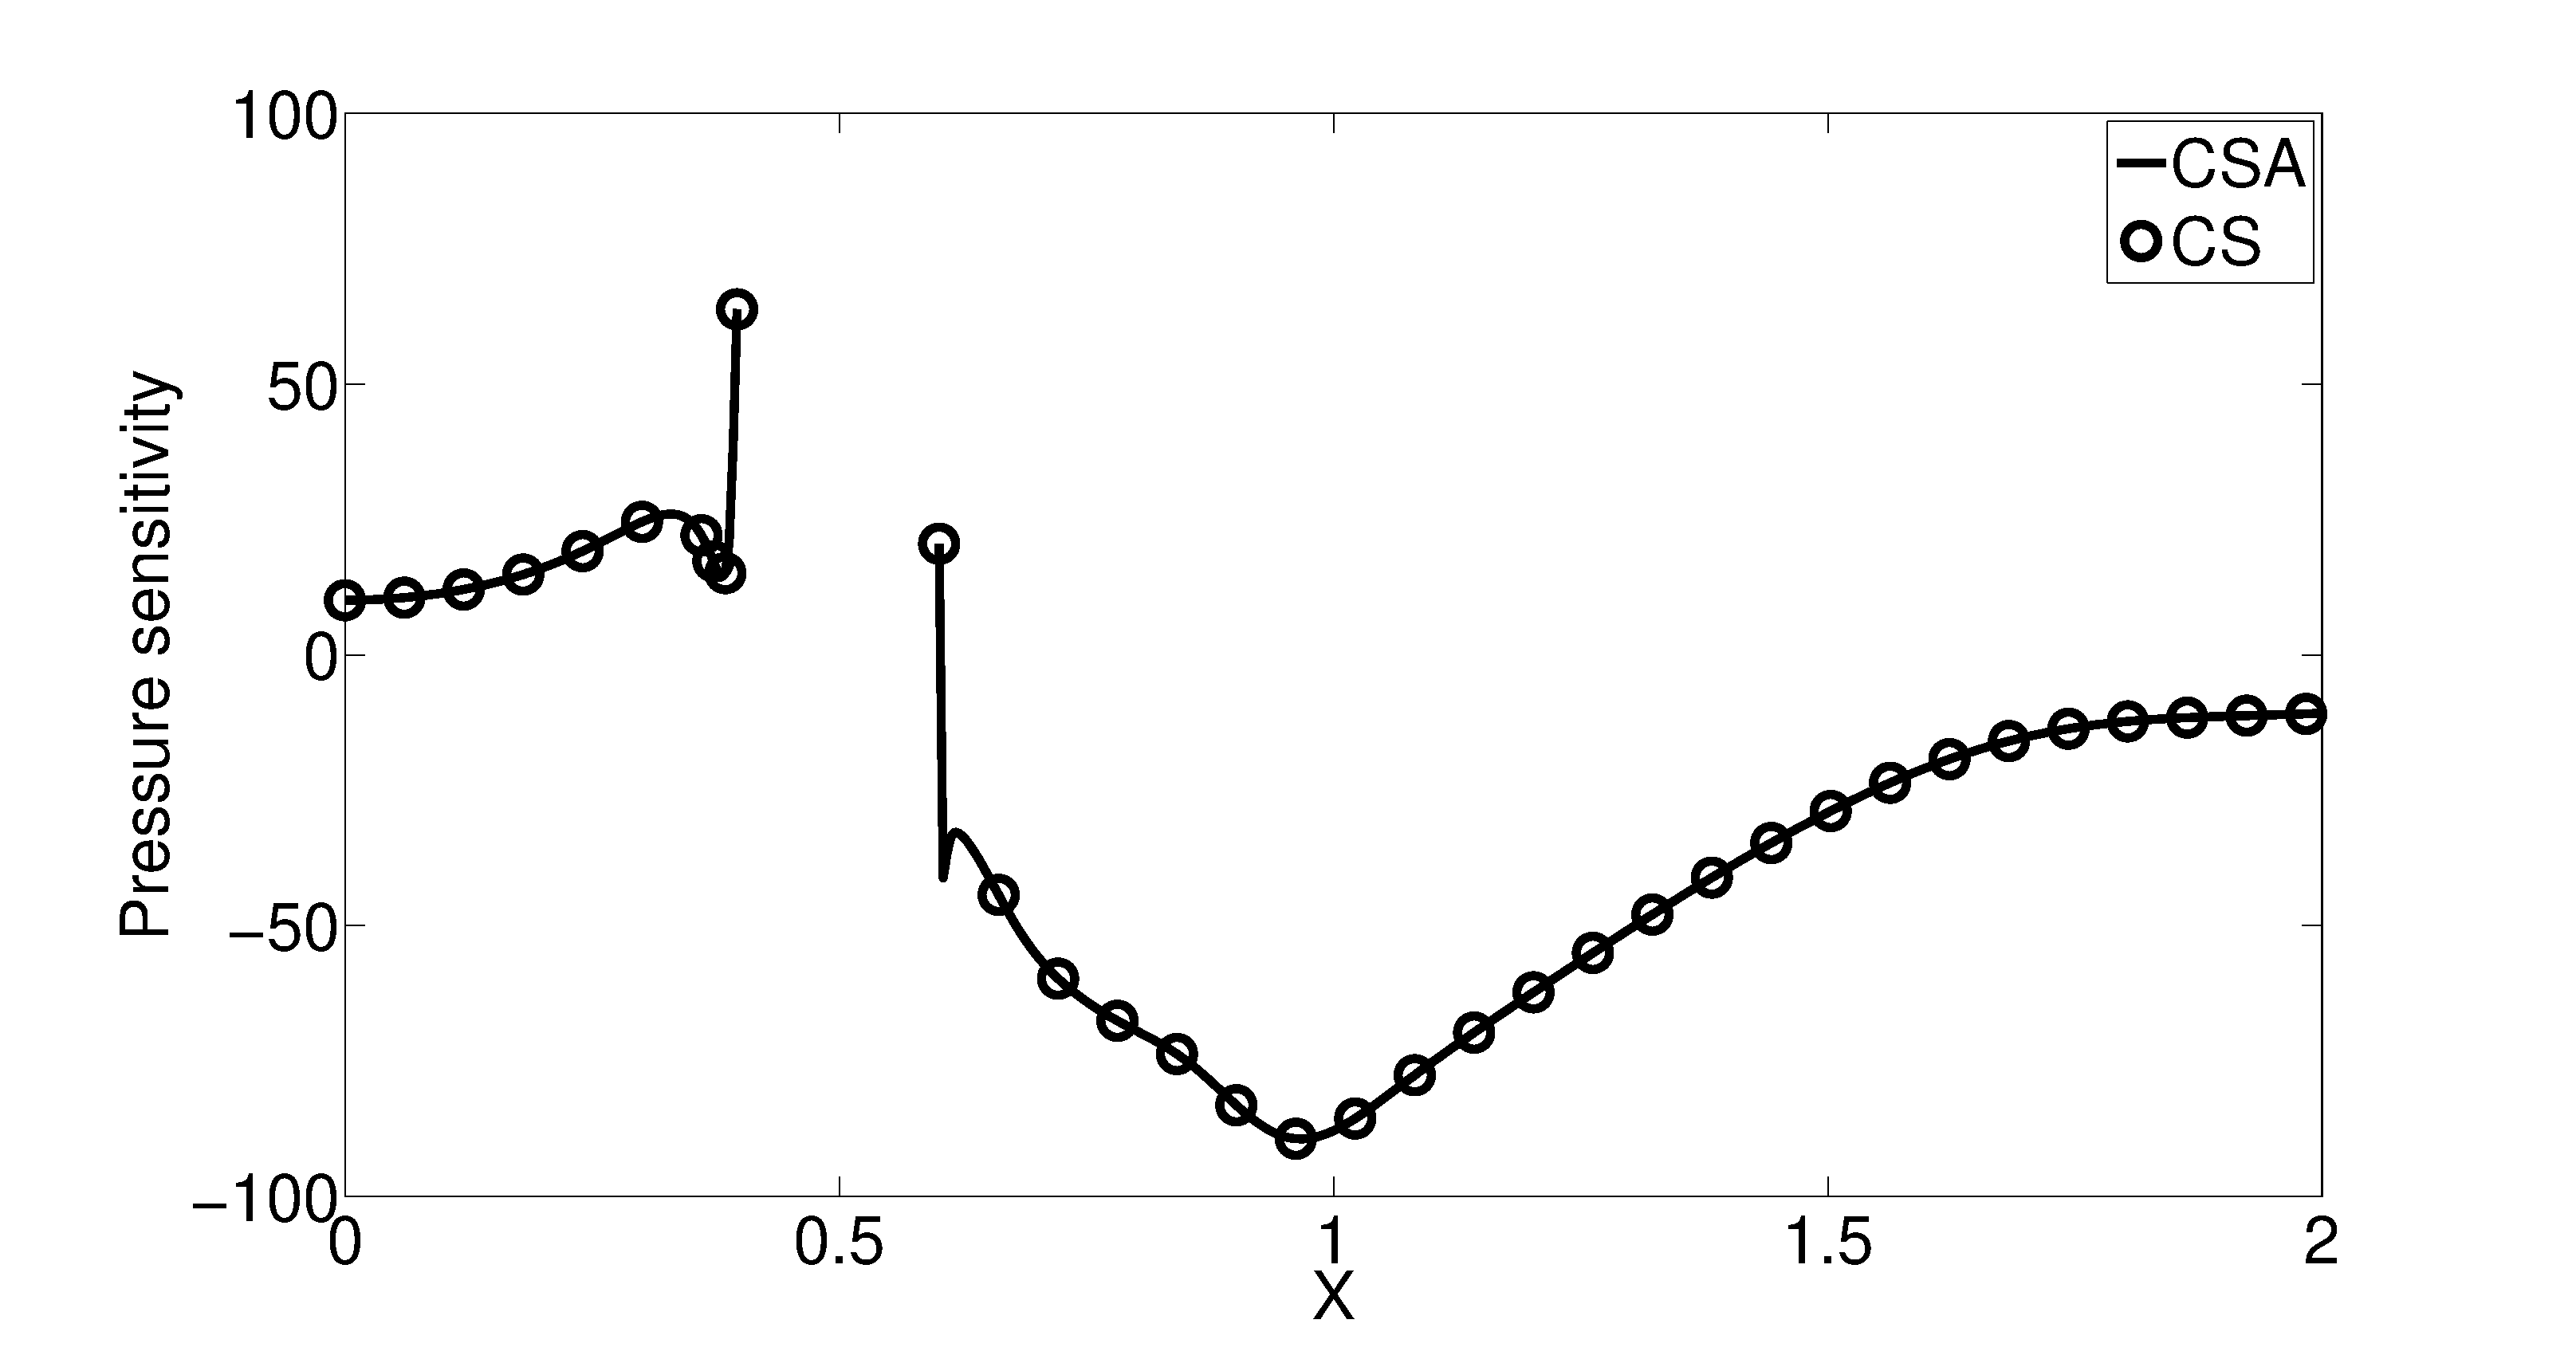
\includegraphics[height=4.0cm]{figure/cylinder/Pp050_RE1000.eps}
	}
	\\
	\subfigure[y = 0.75, Re = 100]
	{
	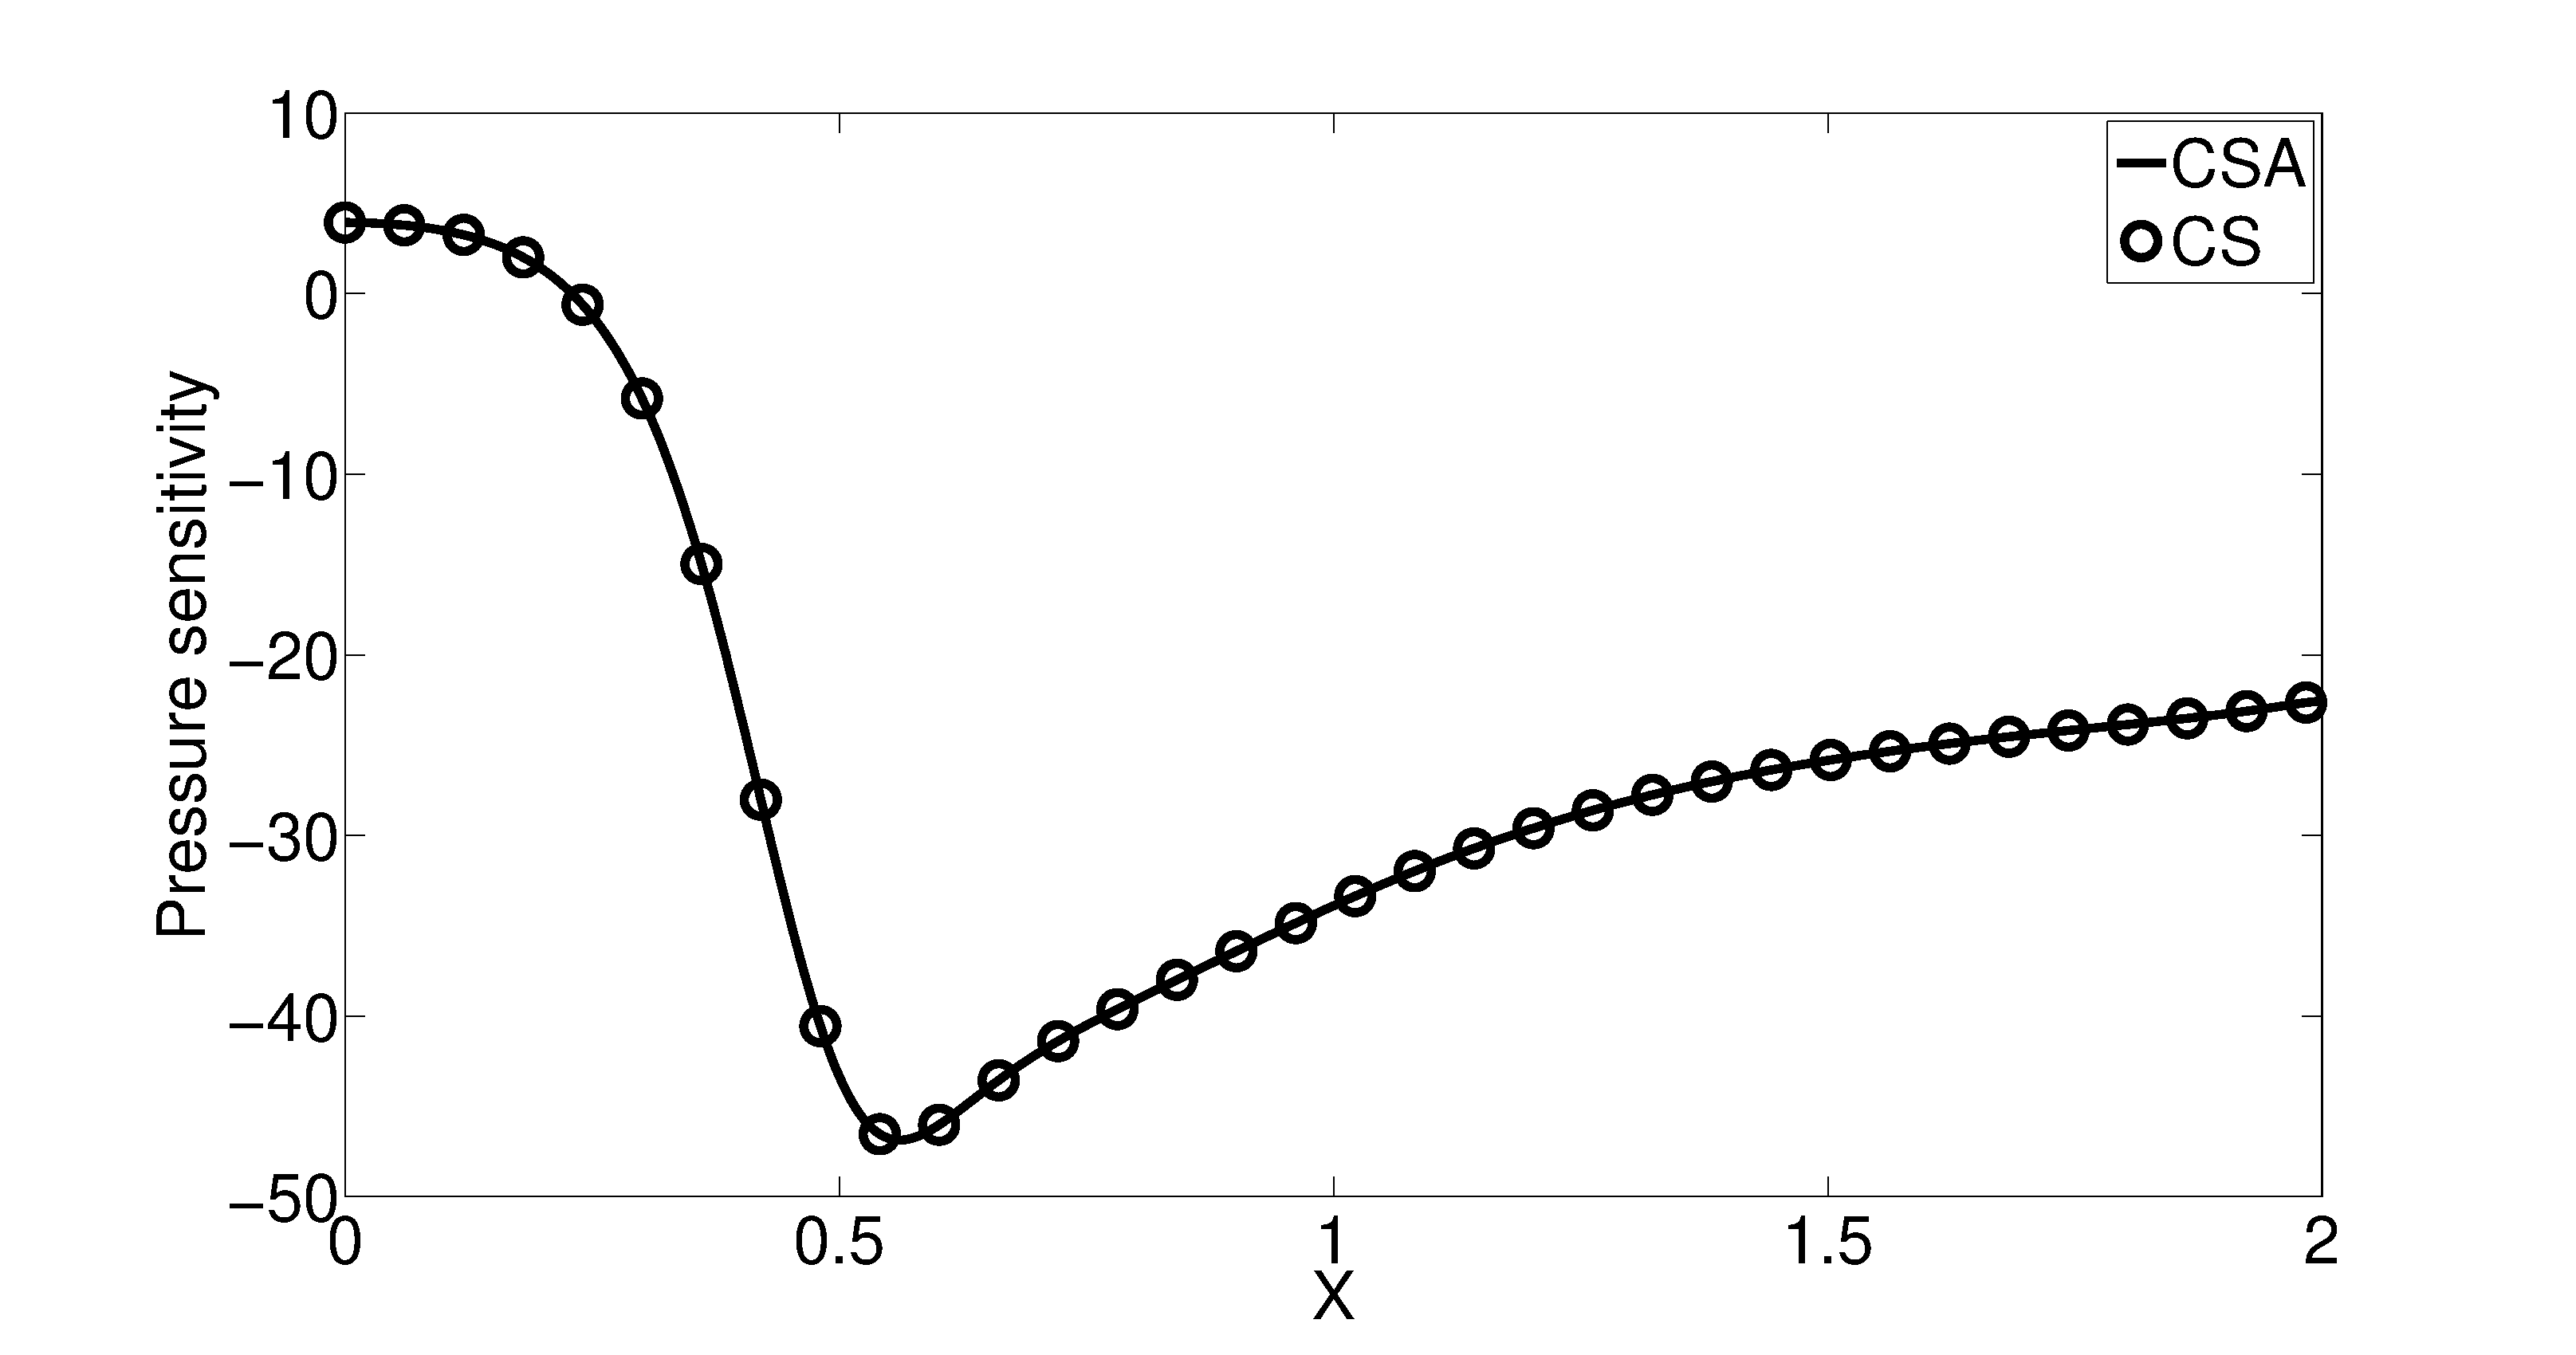
\includegraphics[height=4.0cm]{figure/cylinder/Pp075_RE100.eps}
	}
	\quad
	\subfigure[y = 0.75, Re = 1000]
	{
	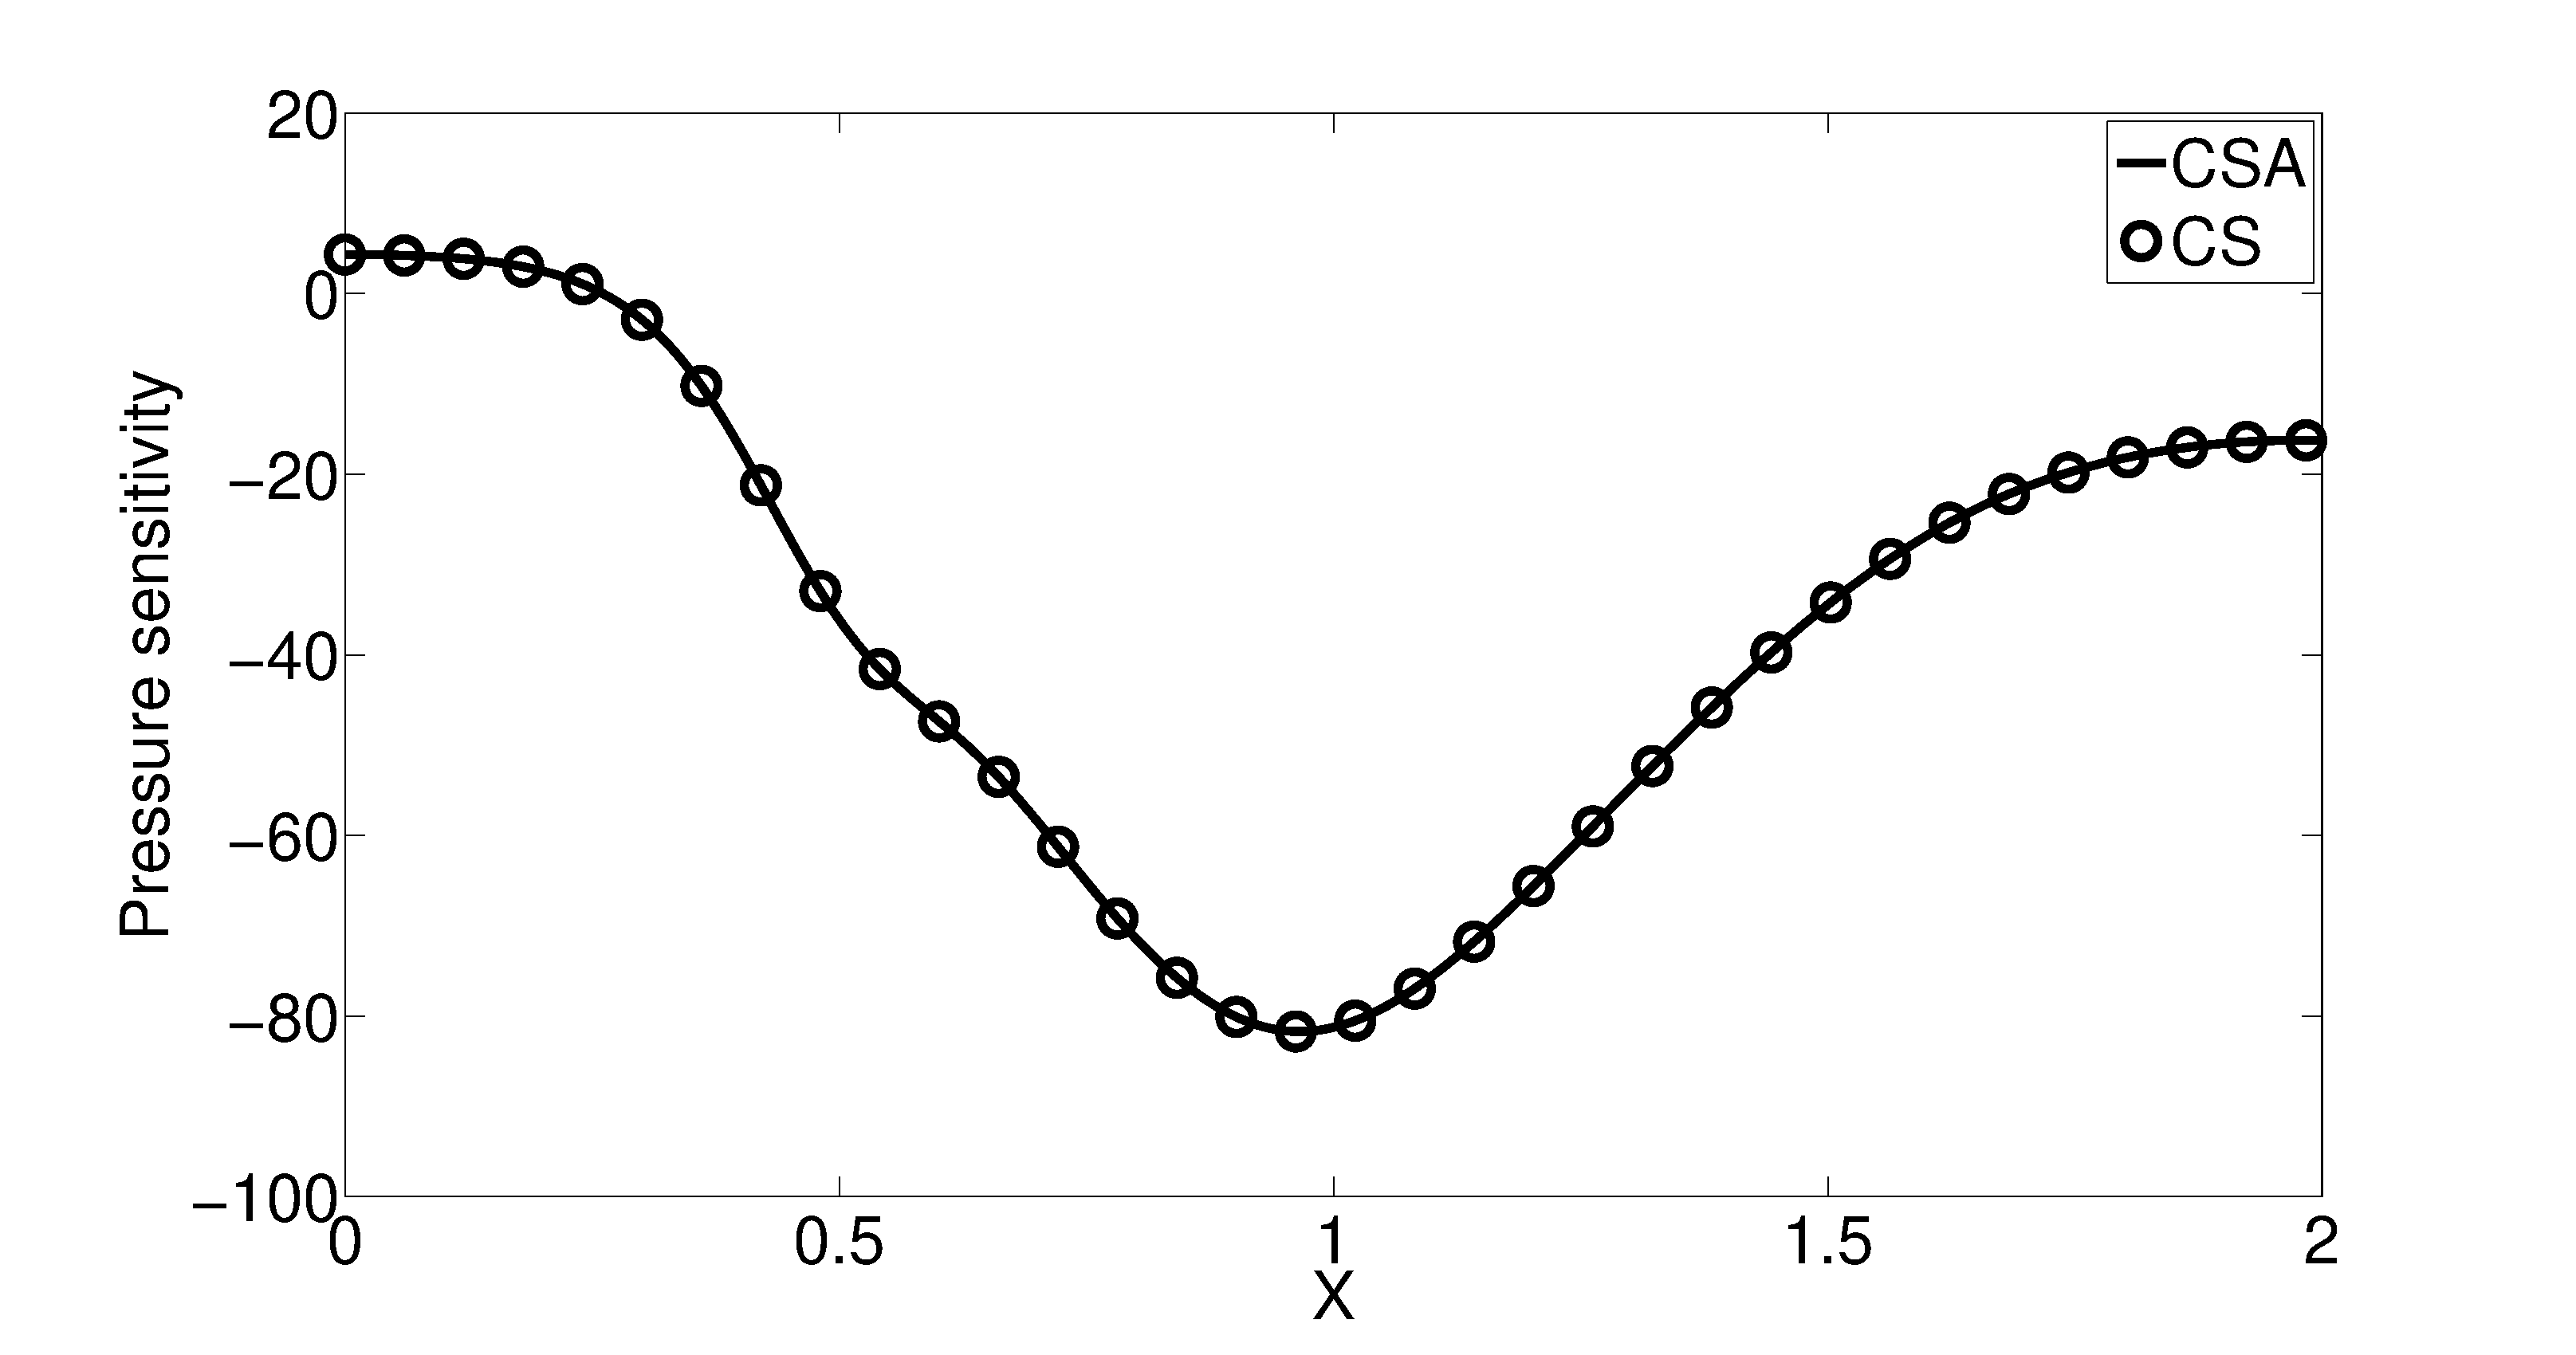
\includegraphics[height=4.0cm]{figure/cylinder/Pp075_RE1000.eps}
	}
	\caption{Pressure sensitivity to cylinder radius for different Reynolds numbers on horizontal sampling line.}
	\label{fig:cylinderPressureSensitivity}
\end{figure}
%

%
\begin{figure}[H]
	\centering
	\subfigure[x = 0.25, Re = 100]
	{
	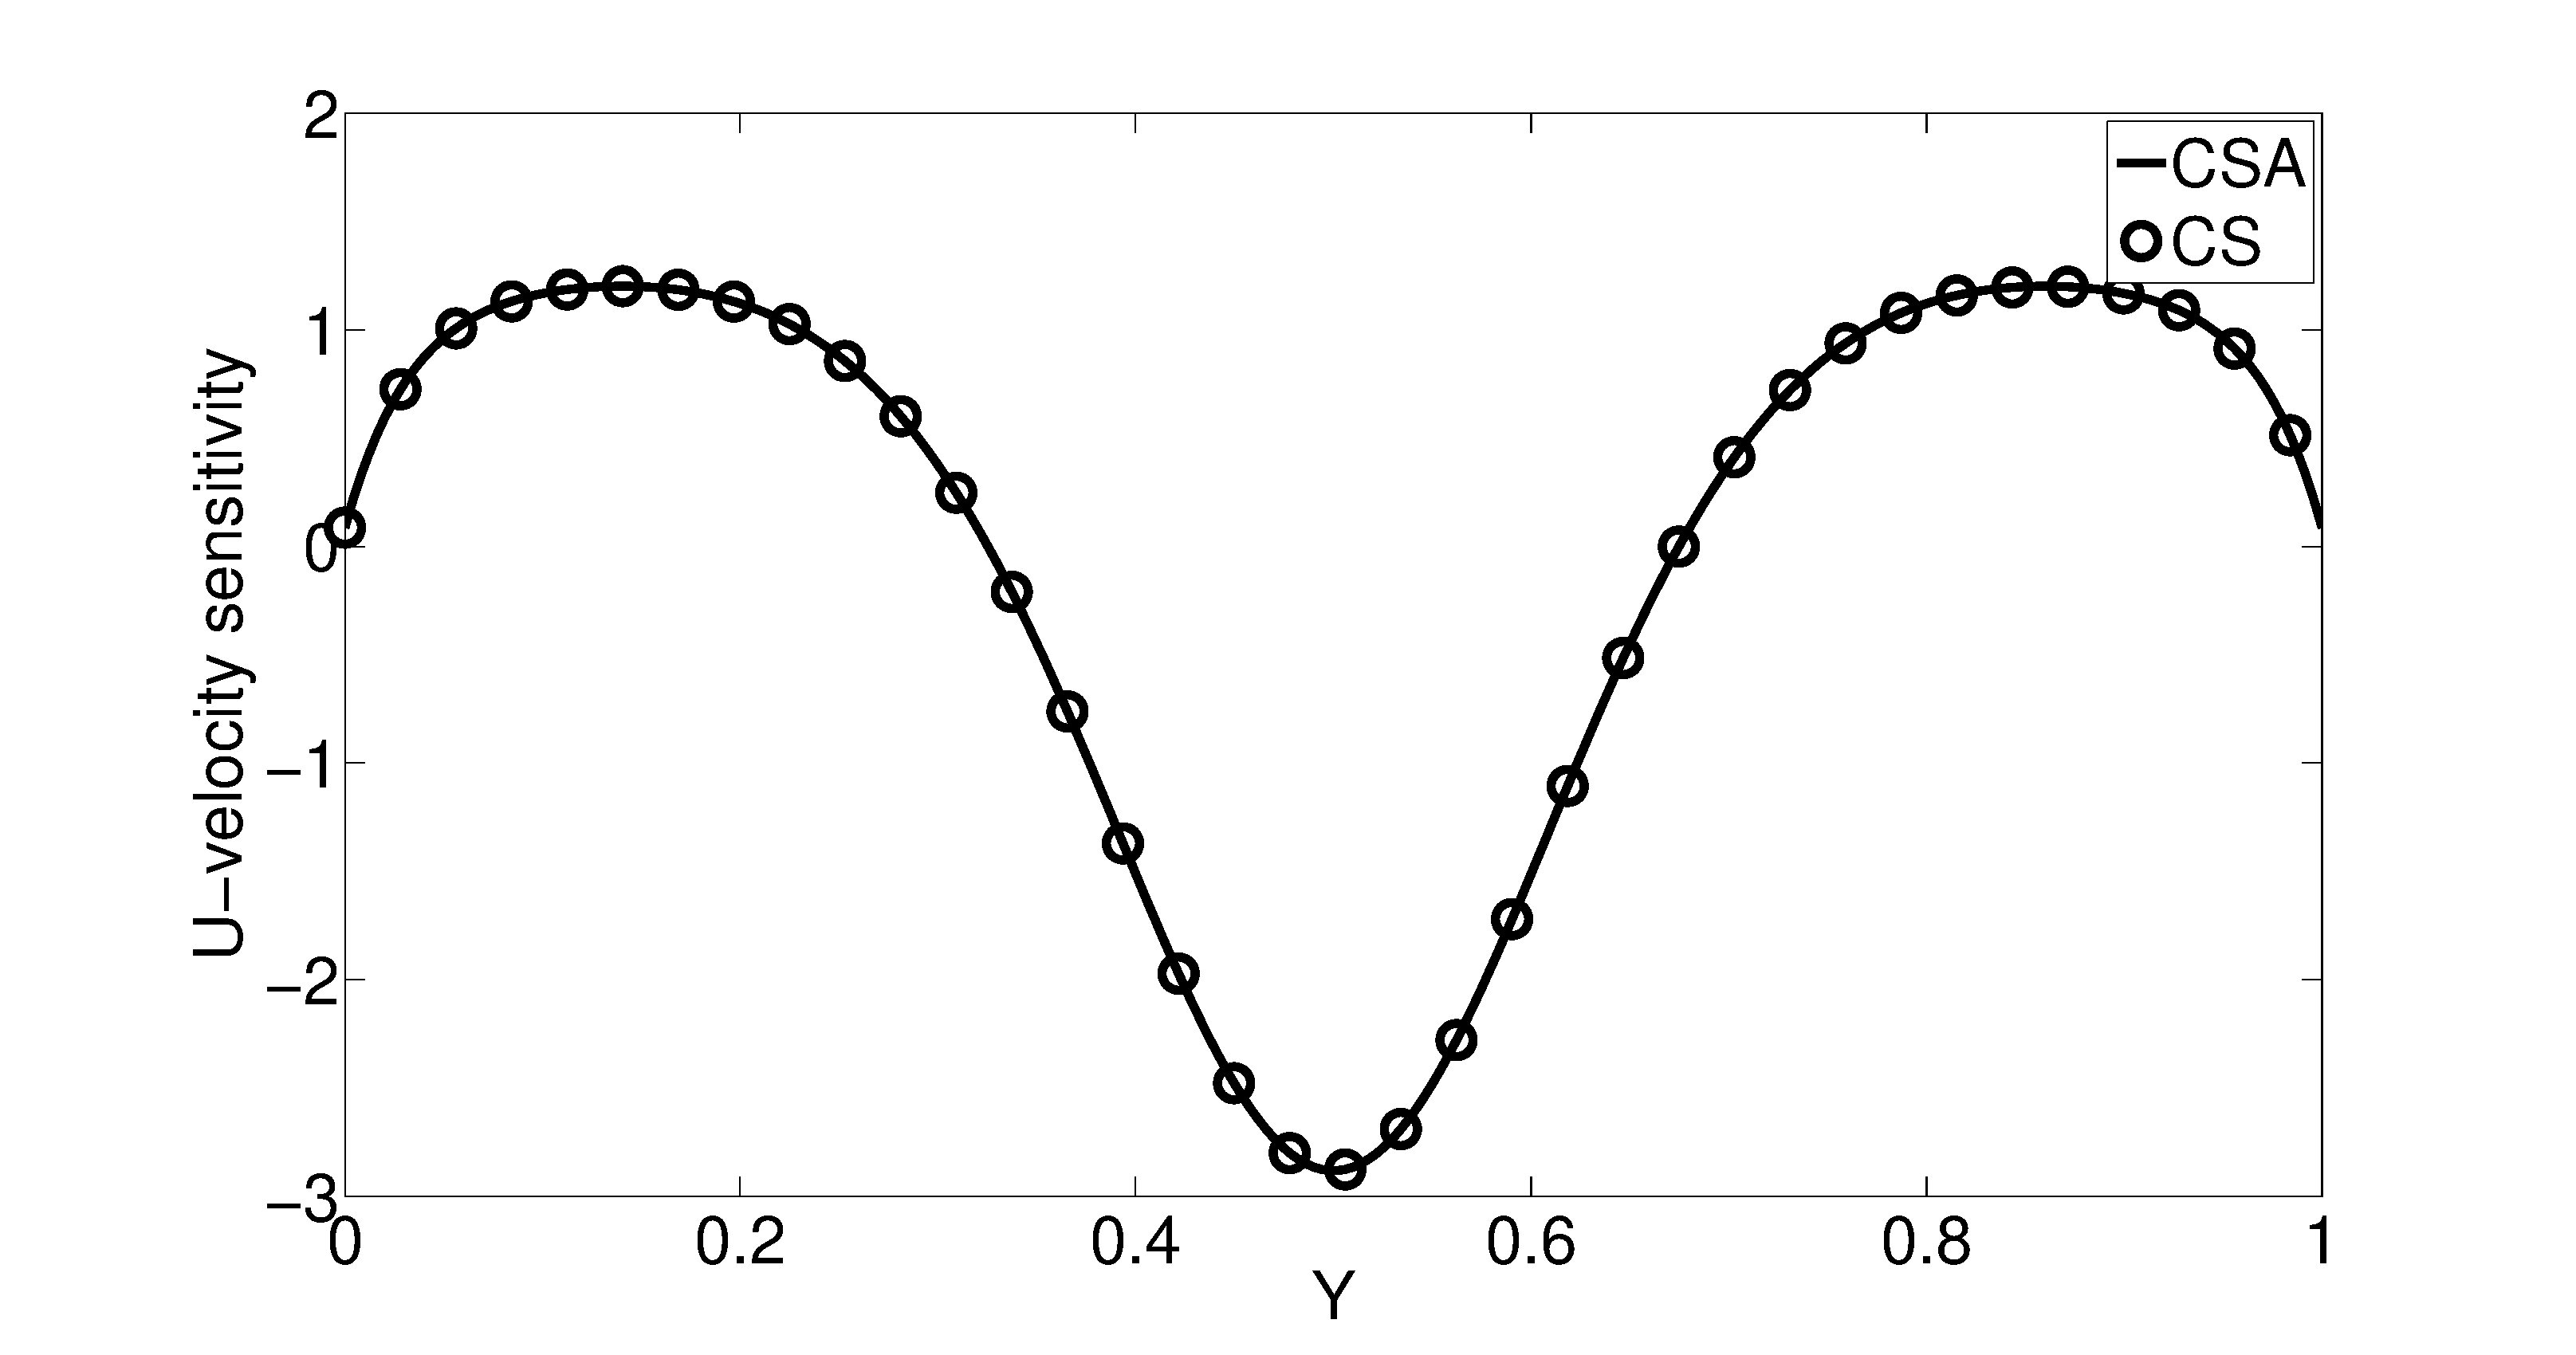
\includegraphics[height=4.0cm]{figure/cylinder/Up025_RE100.eps}
	}
	\quad
	\subfigure[x = 0.25, Re = 1000]
	{
	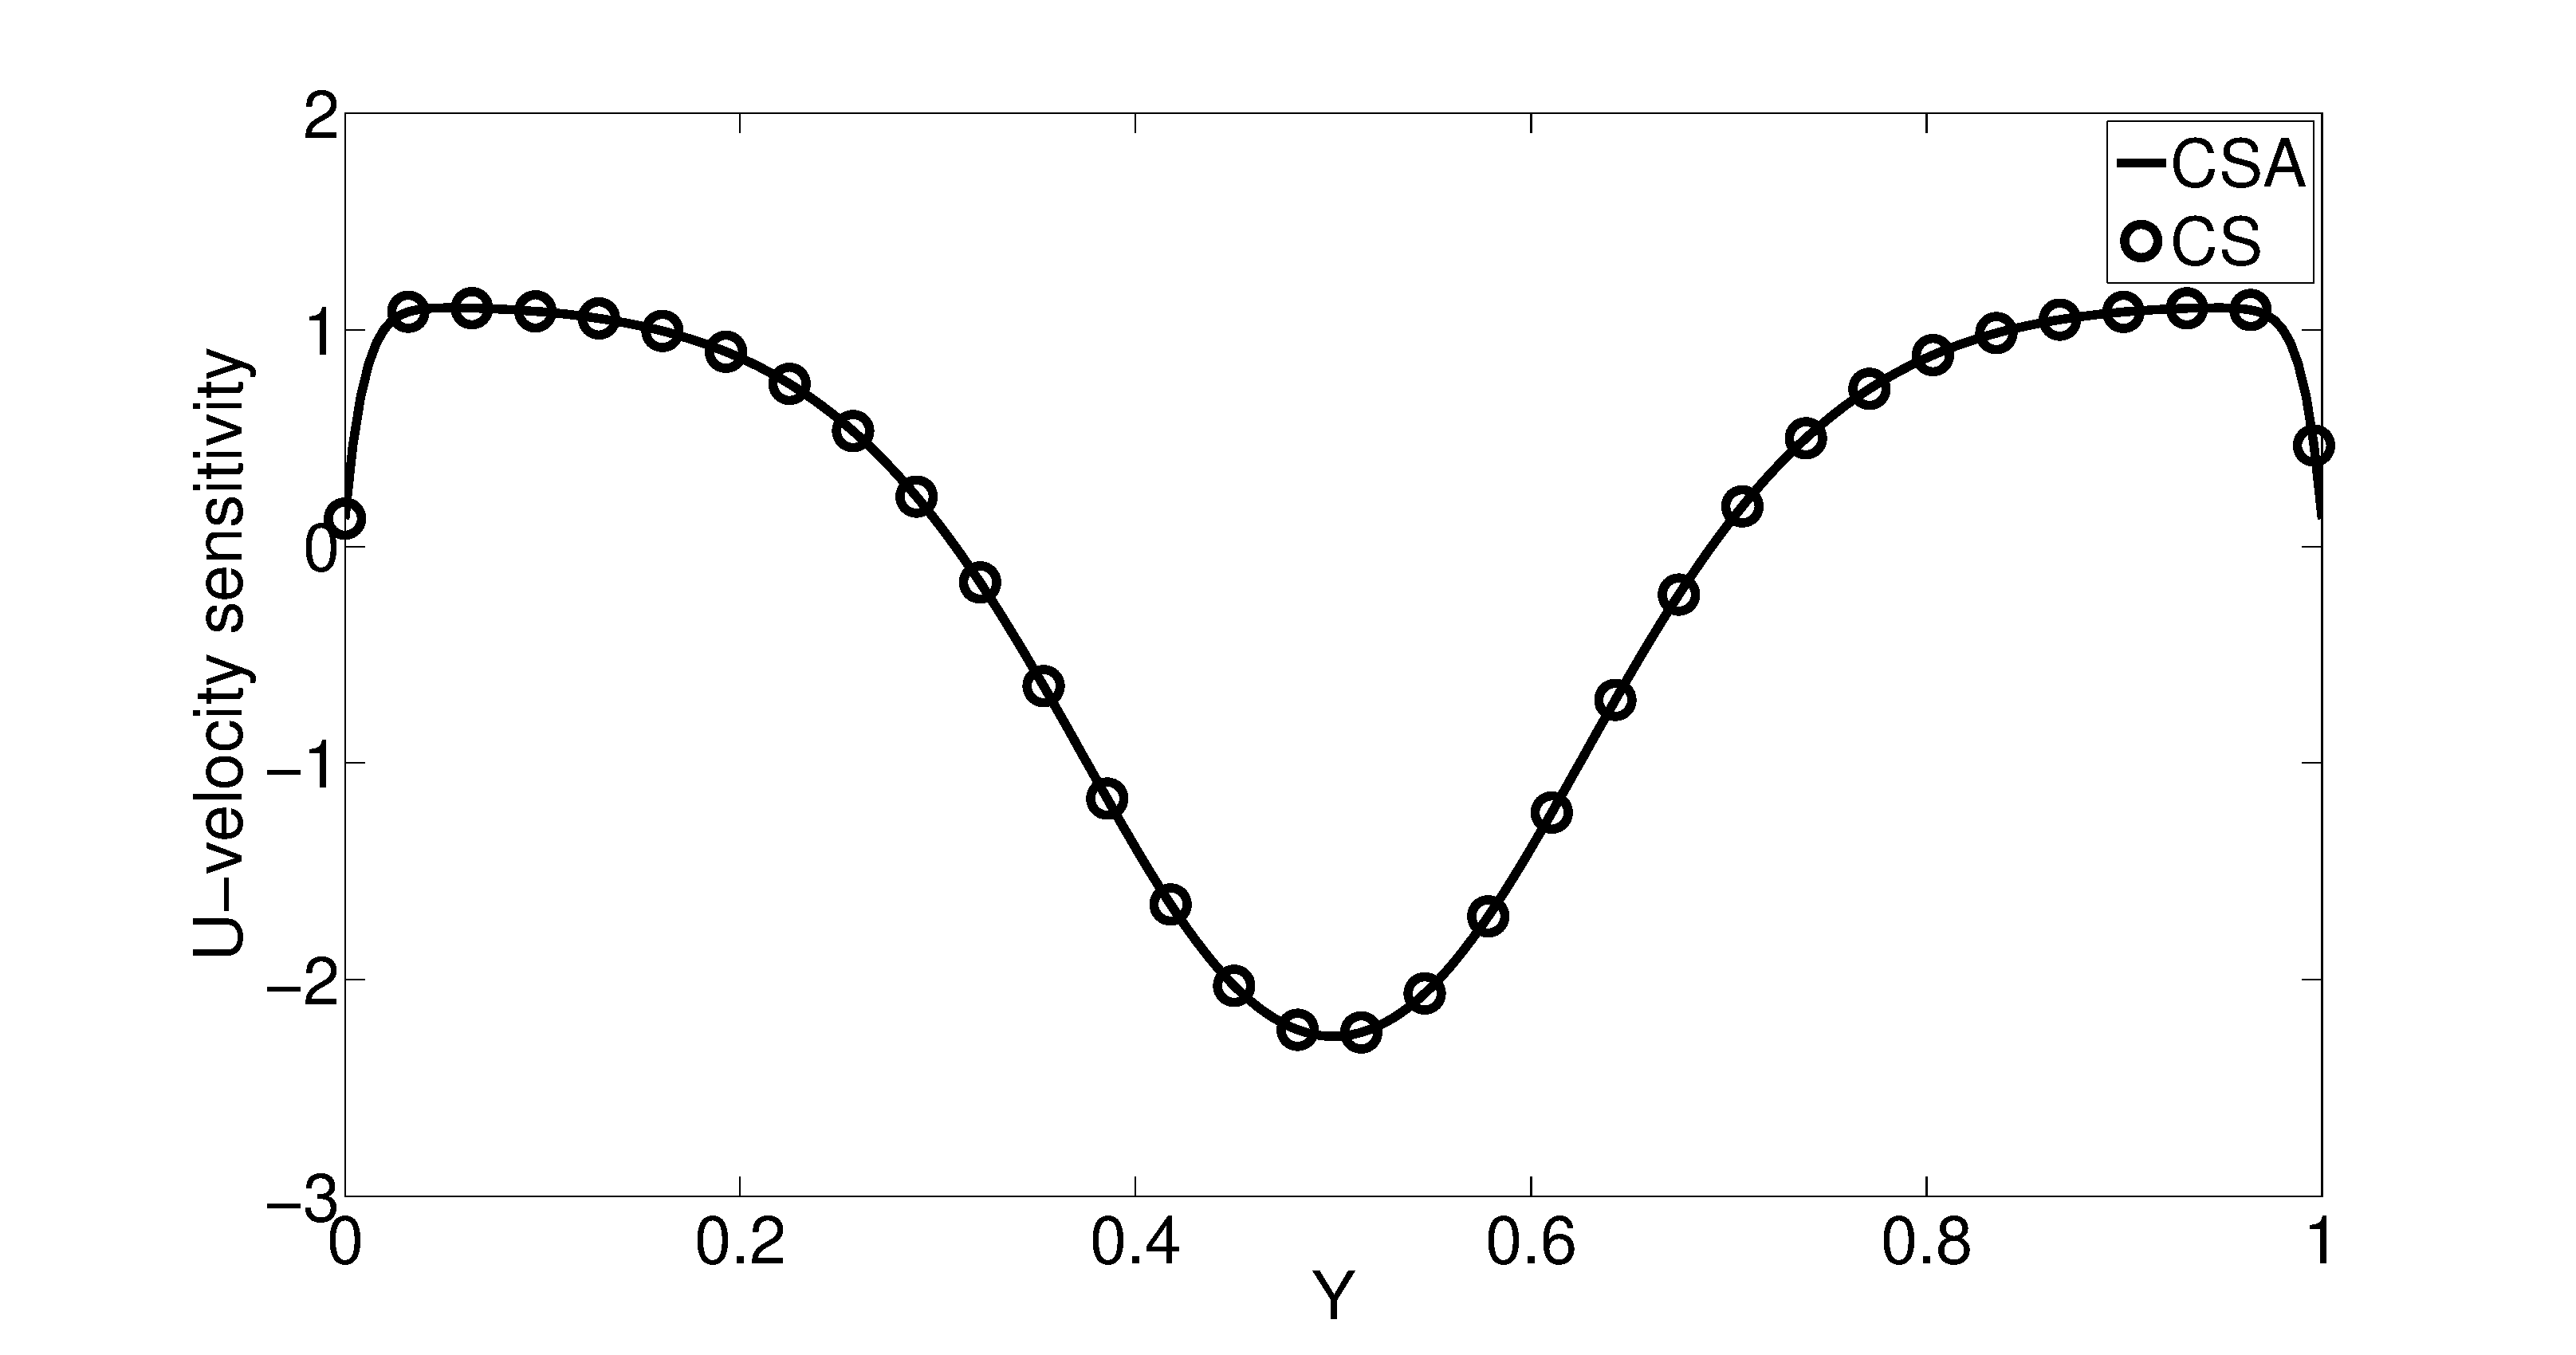
\includegraphics[height=4.0cm]{figure/cylinder/Up025_RE1000.eps}
	}
	\\
	\subfigure[x = 0.5, Re = 100]
	{
	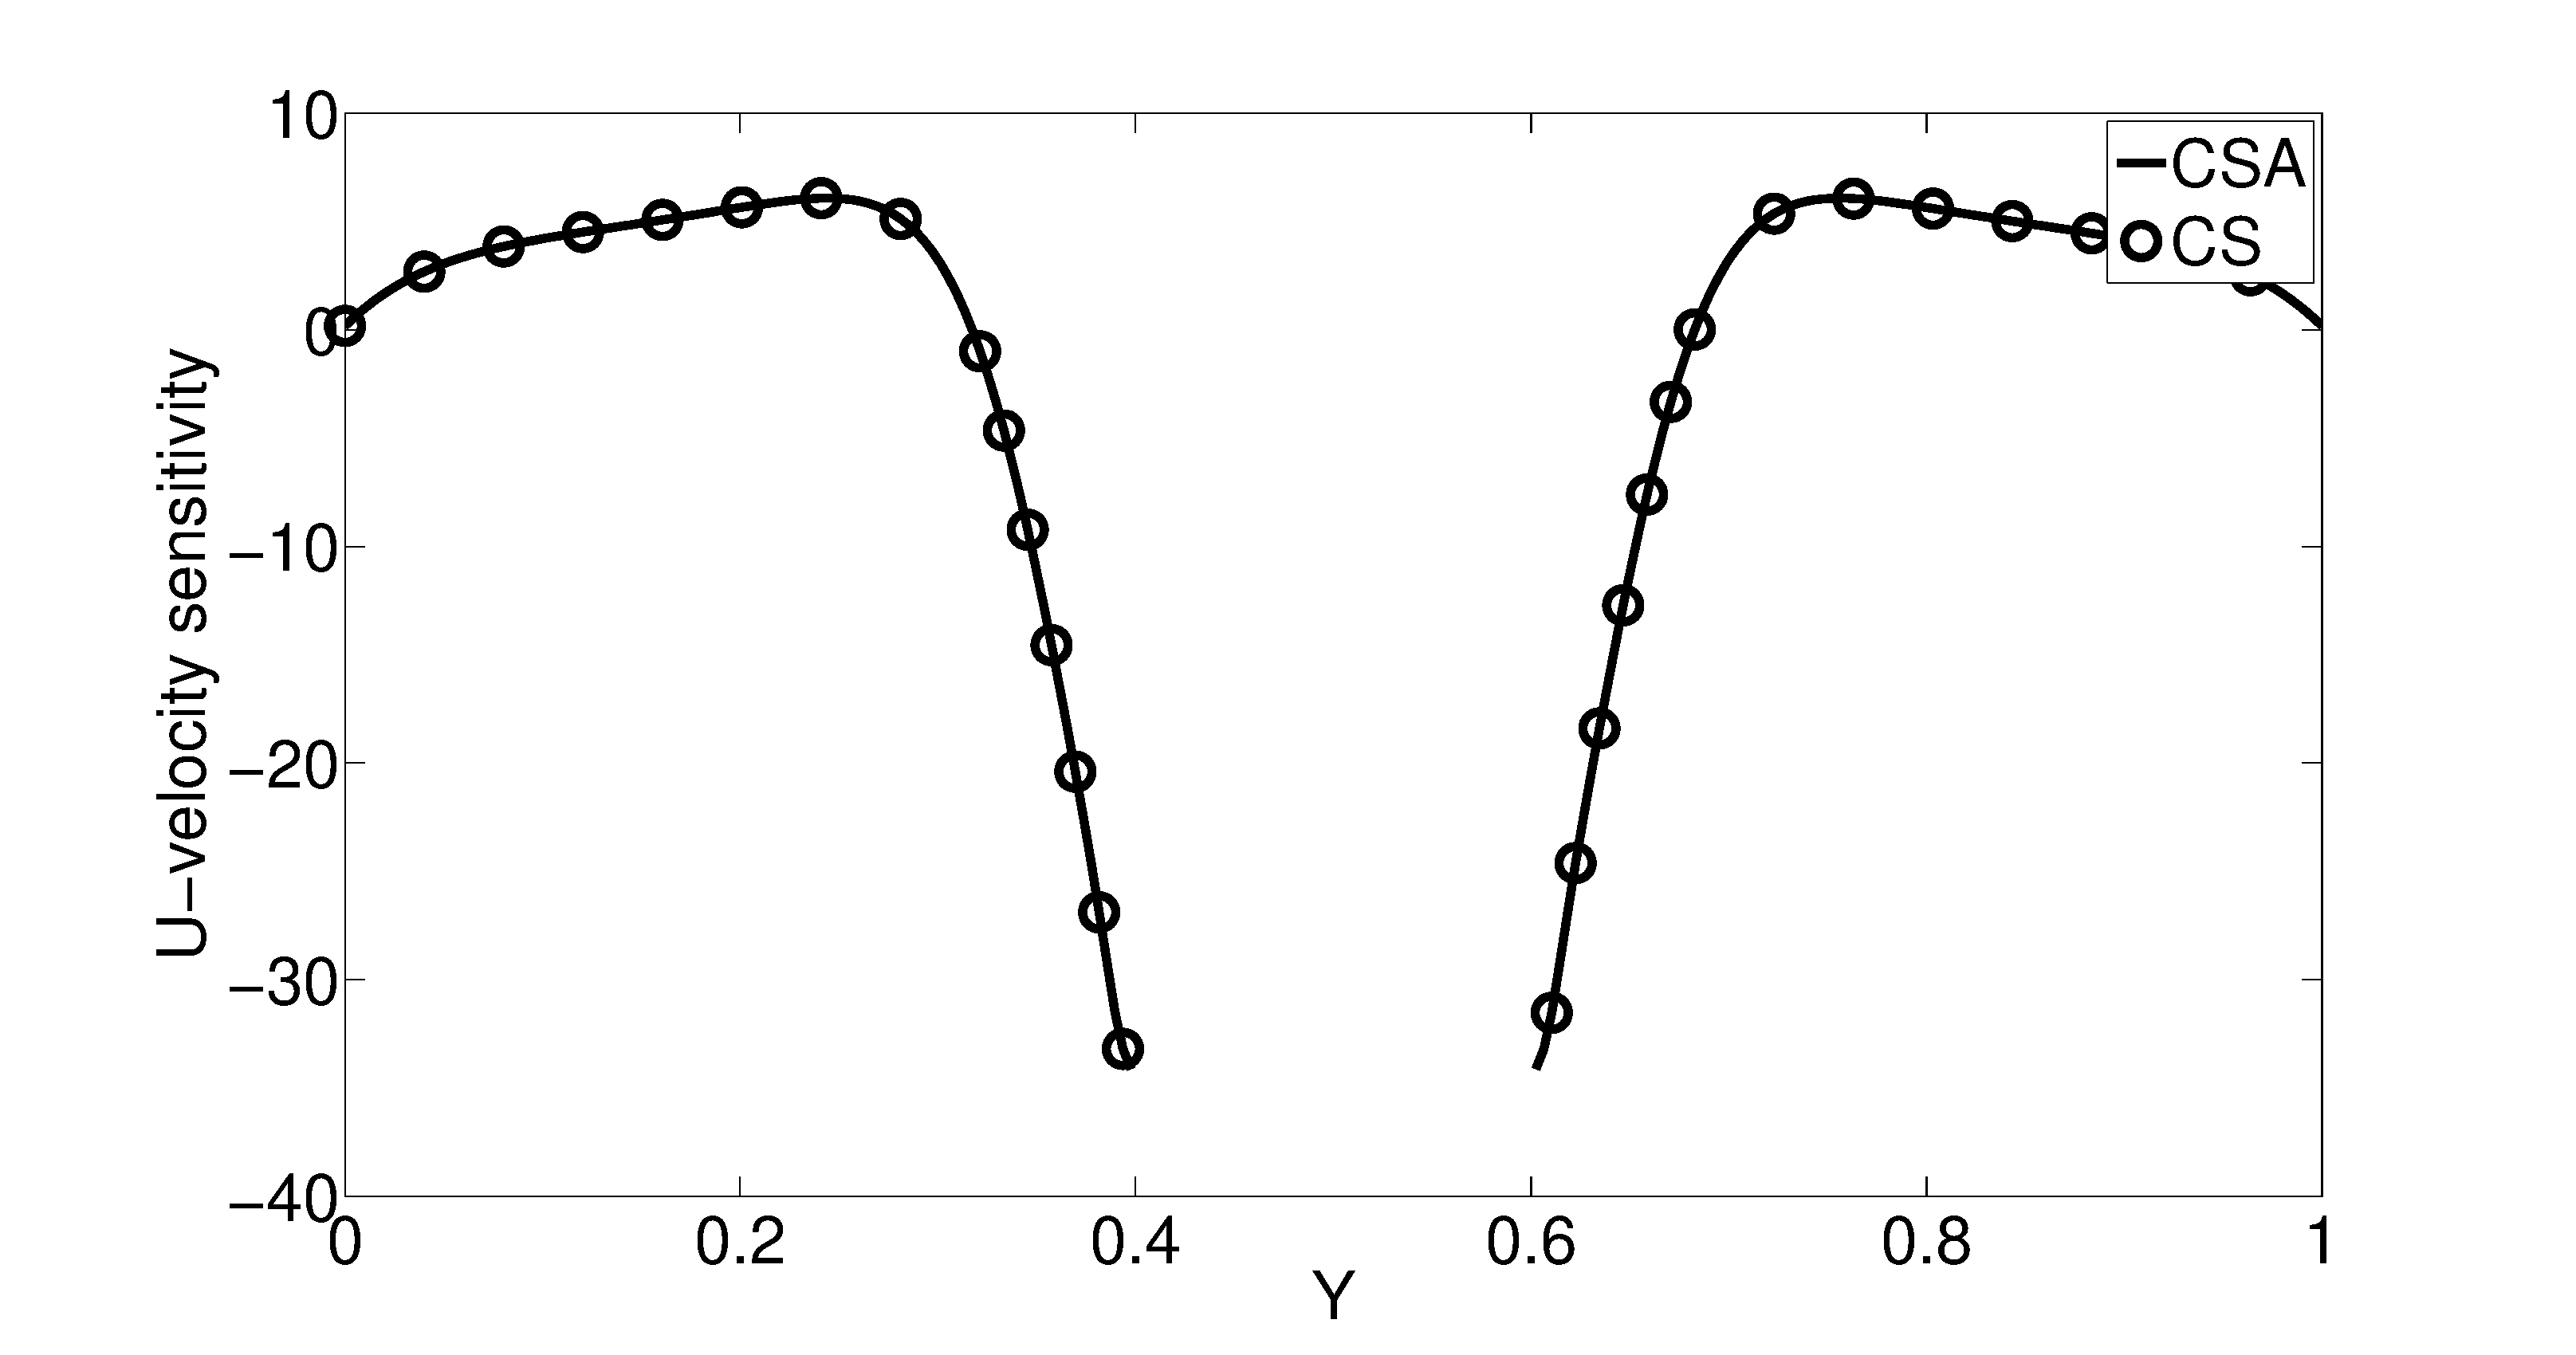
\includegraphics[height=4.0cm]{figure/cylinder/Up050_RE100.eps}
	}
	\quad
	\subfigure[x = 0.5, Re = 1000]
	{
	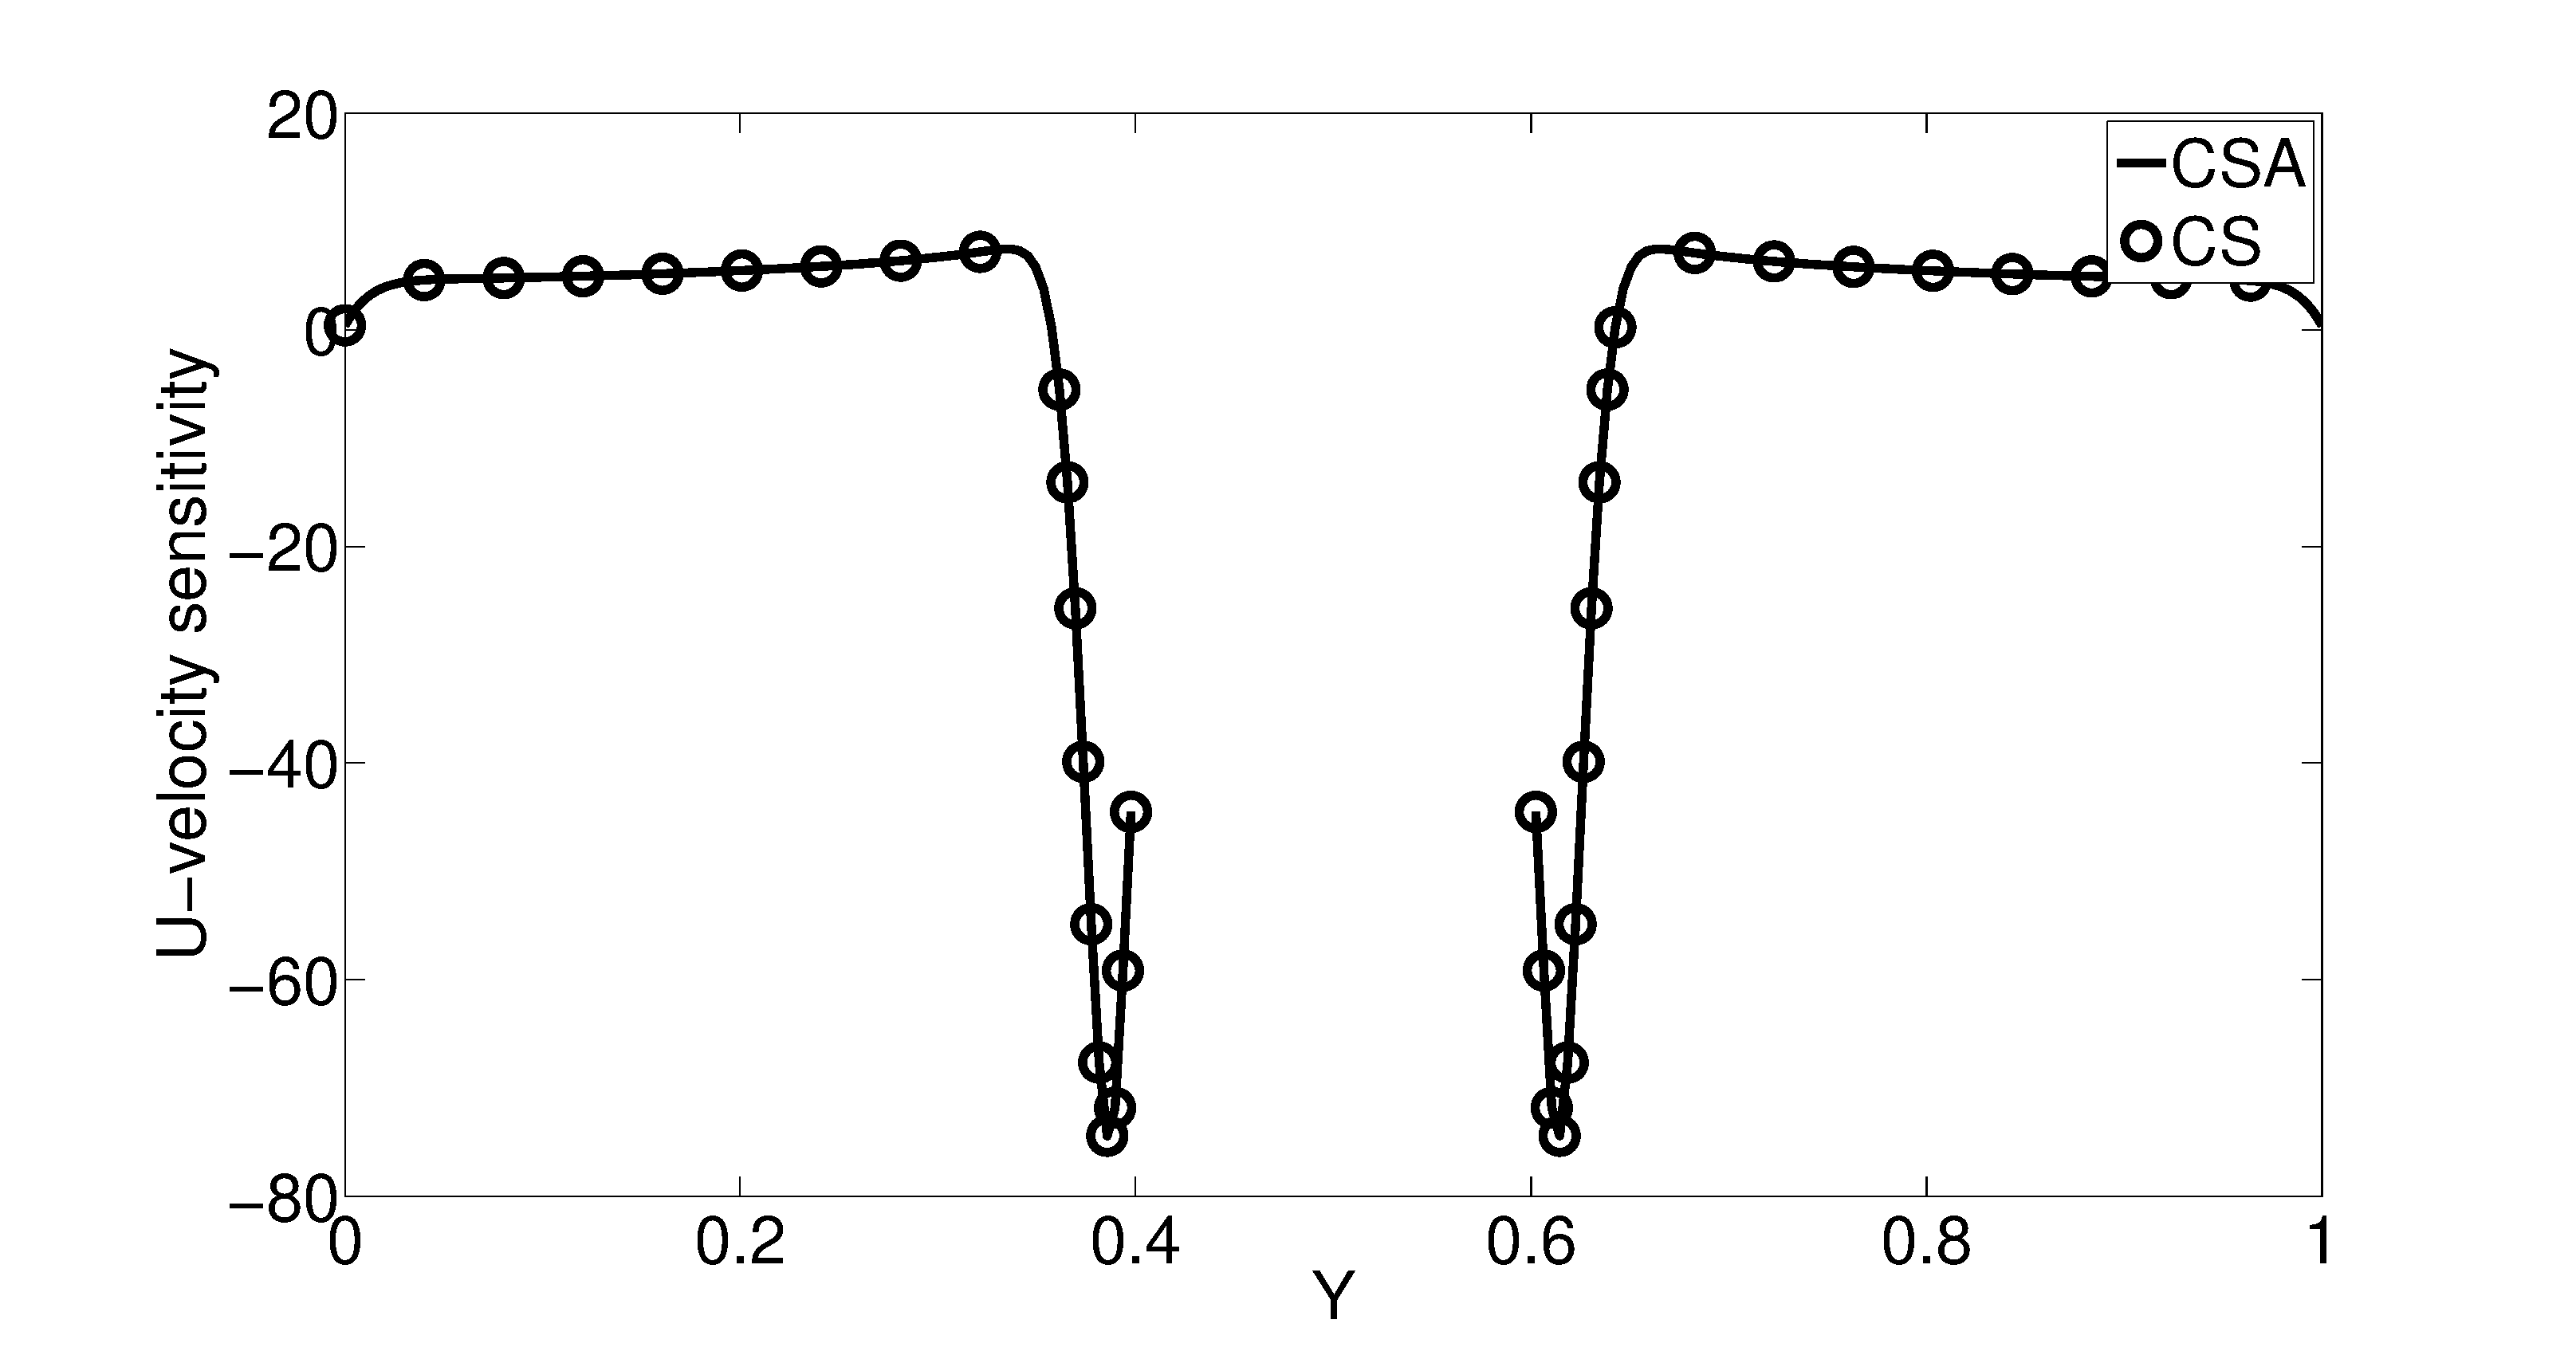
\includegraphics[height=4.0cm]{figure/cylinder/Up050_RE1000.eps}
	}
	\\
	\subfigure[x = 0.75, Re = 100]
	{
	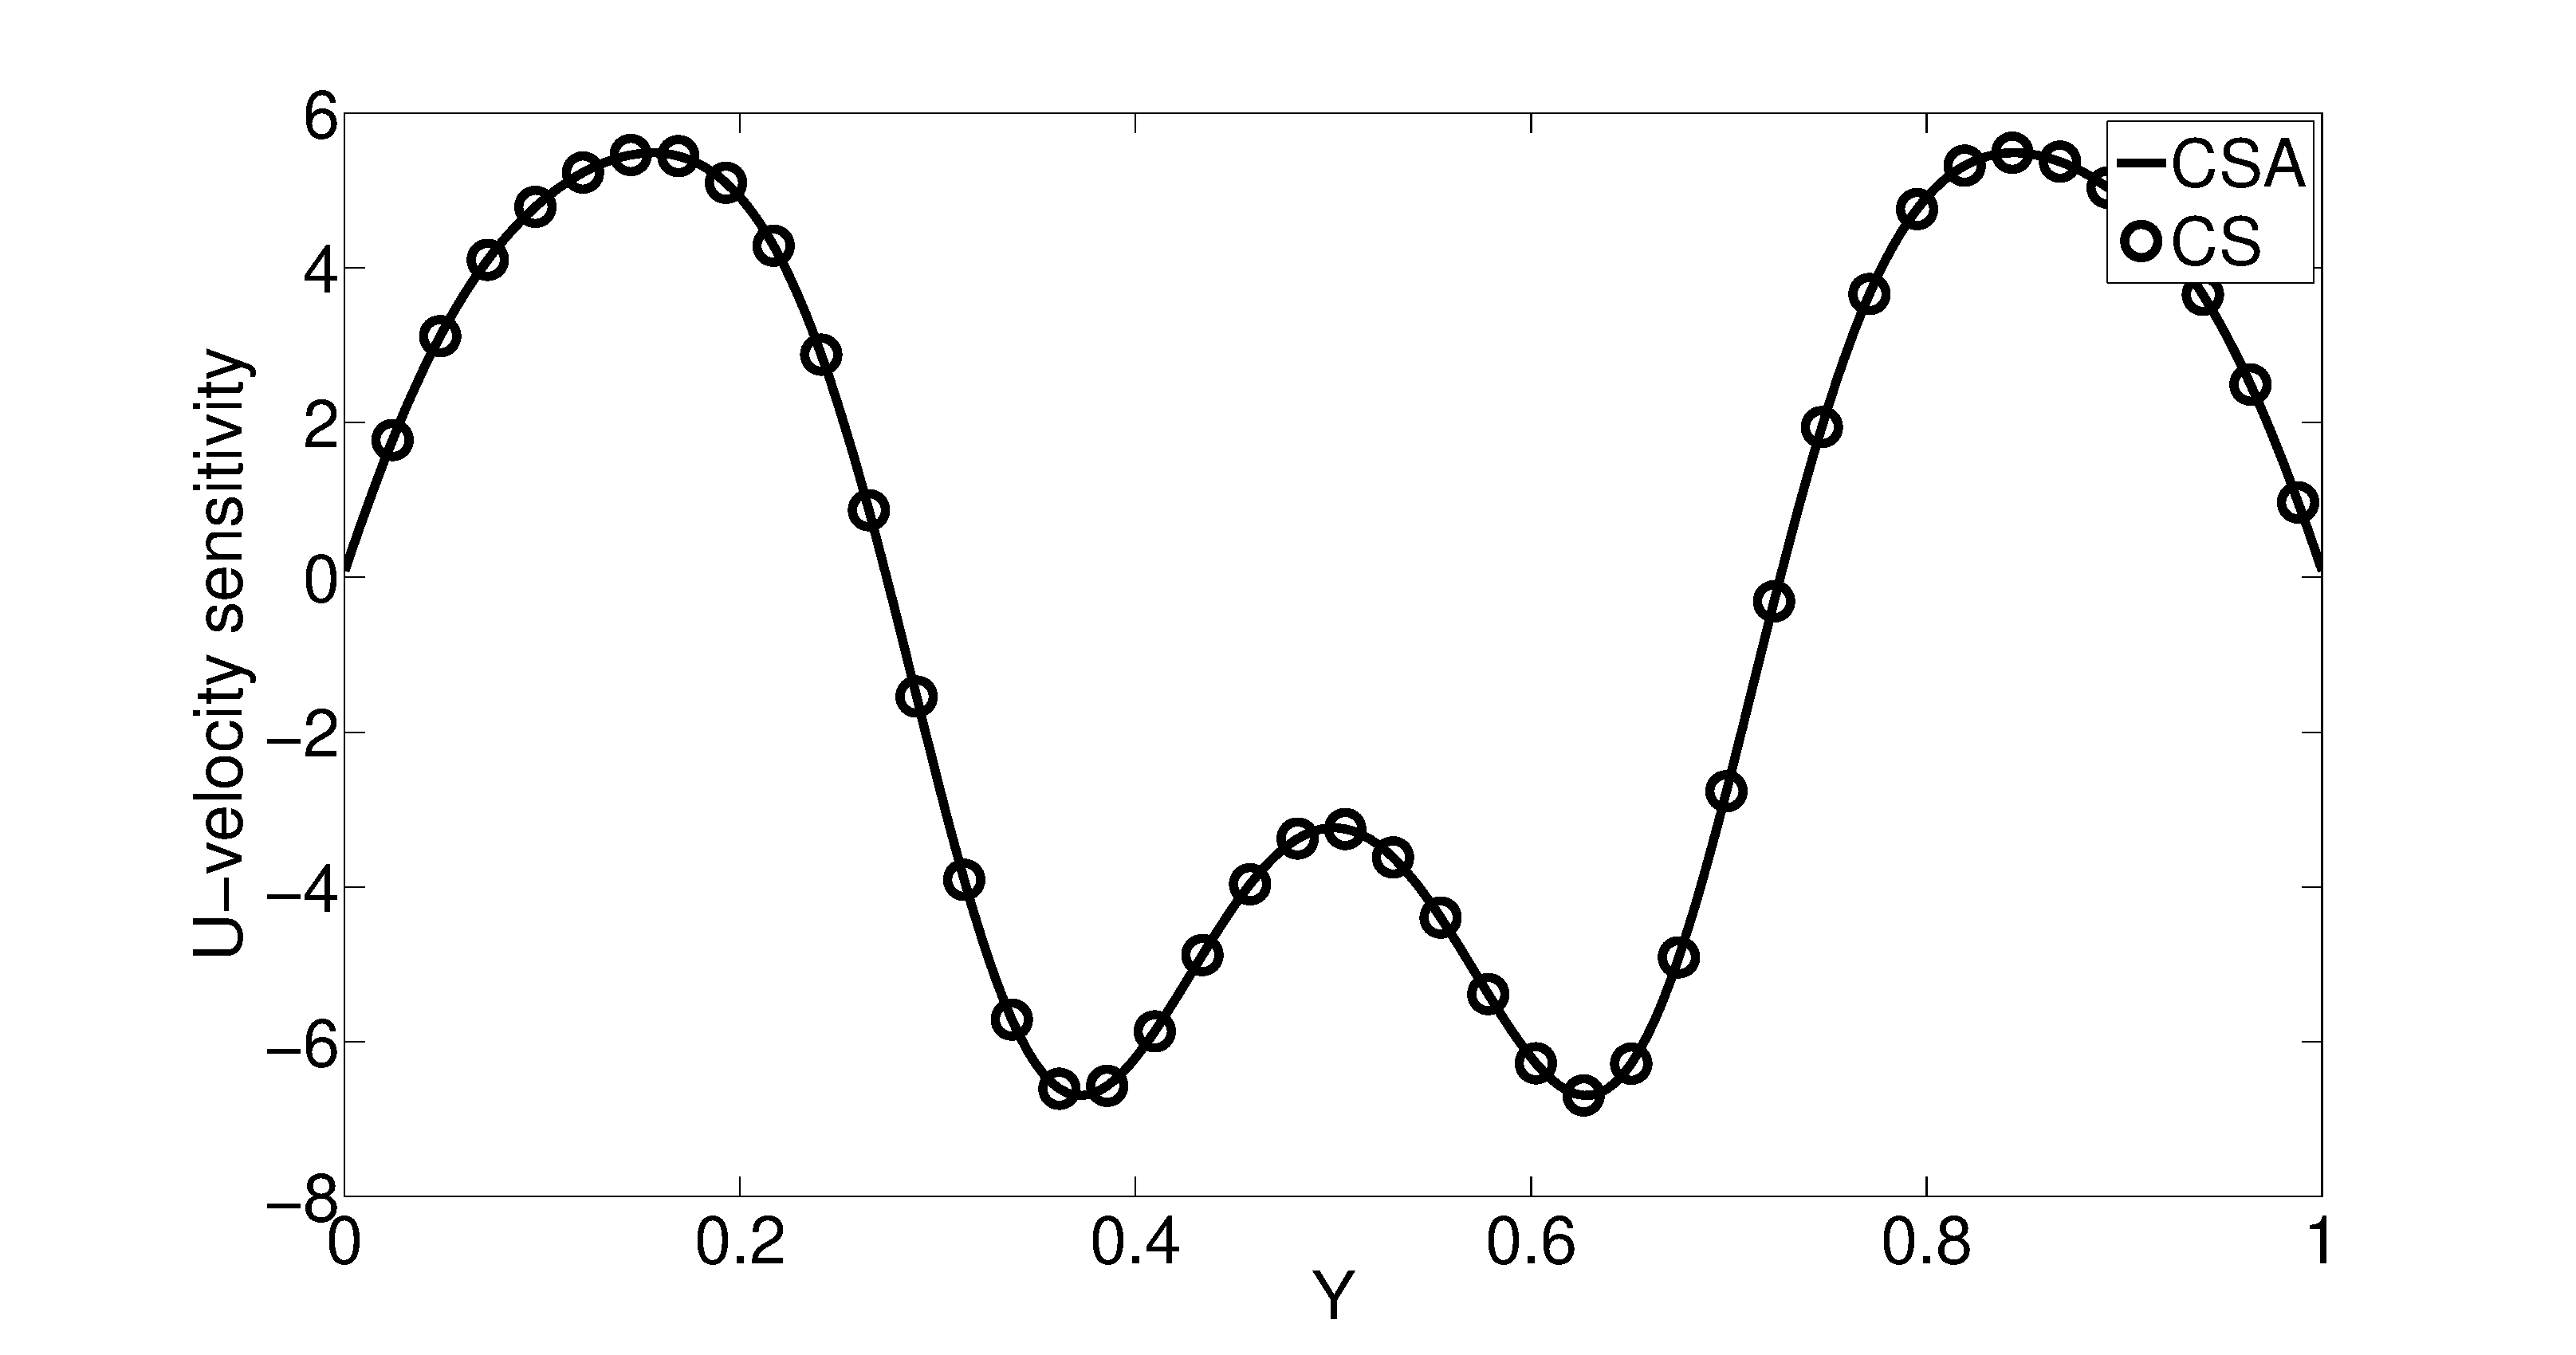
\includegraphics[height=4.0cm]{figure/cylinder/Up075_RE100.eps}
	}
	\quad
	\subfigure[x = 0.75, Re = 1000]
	{
	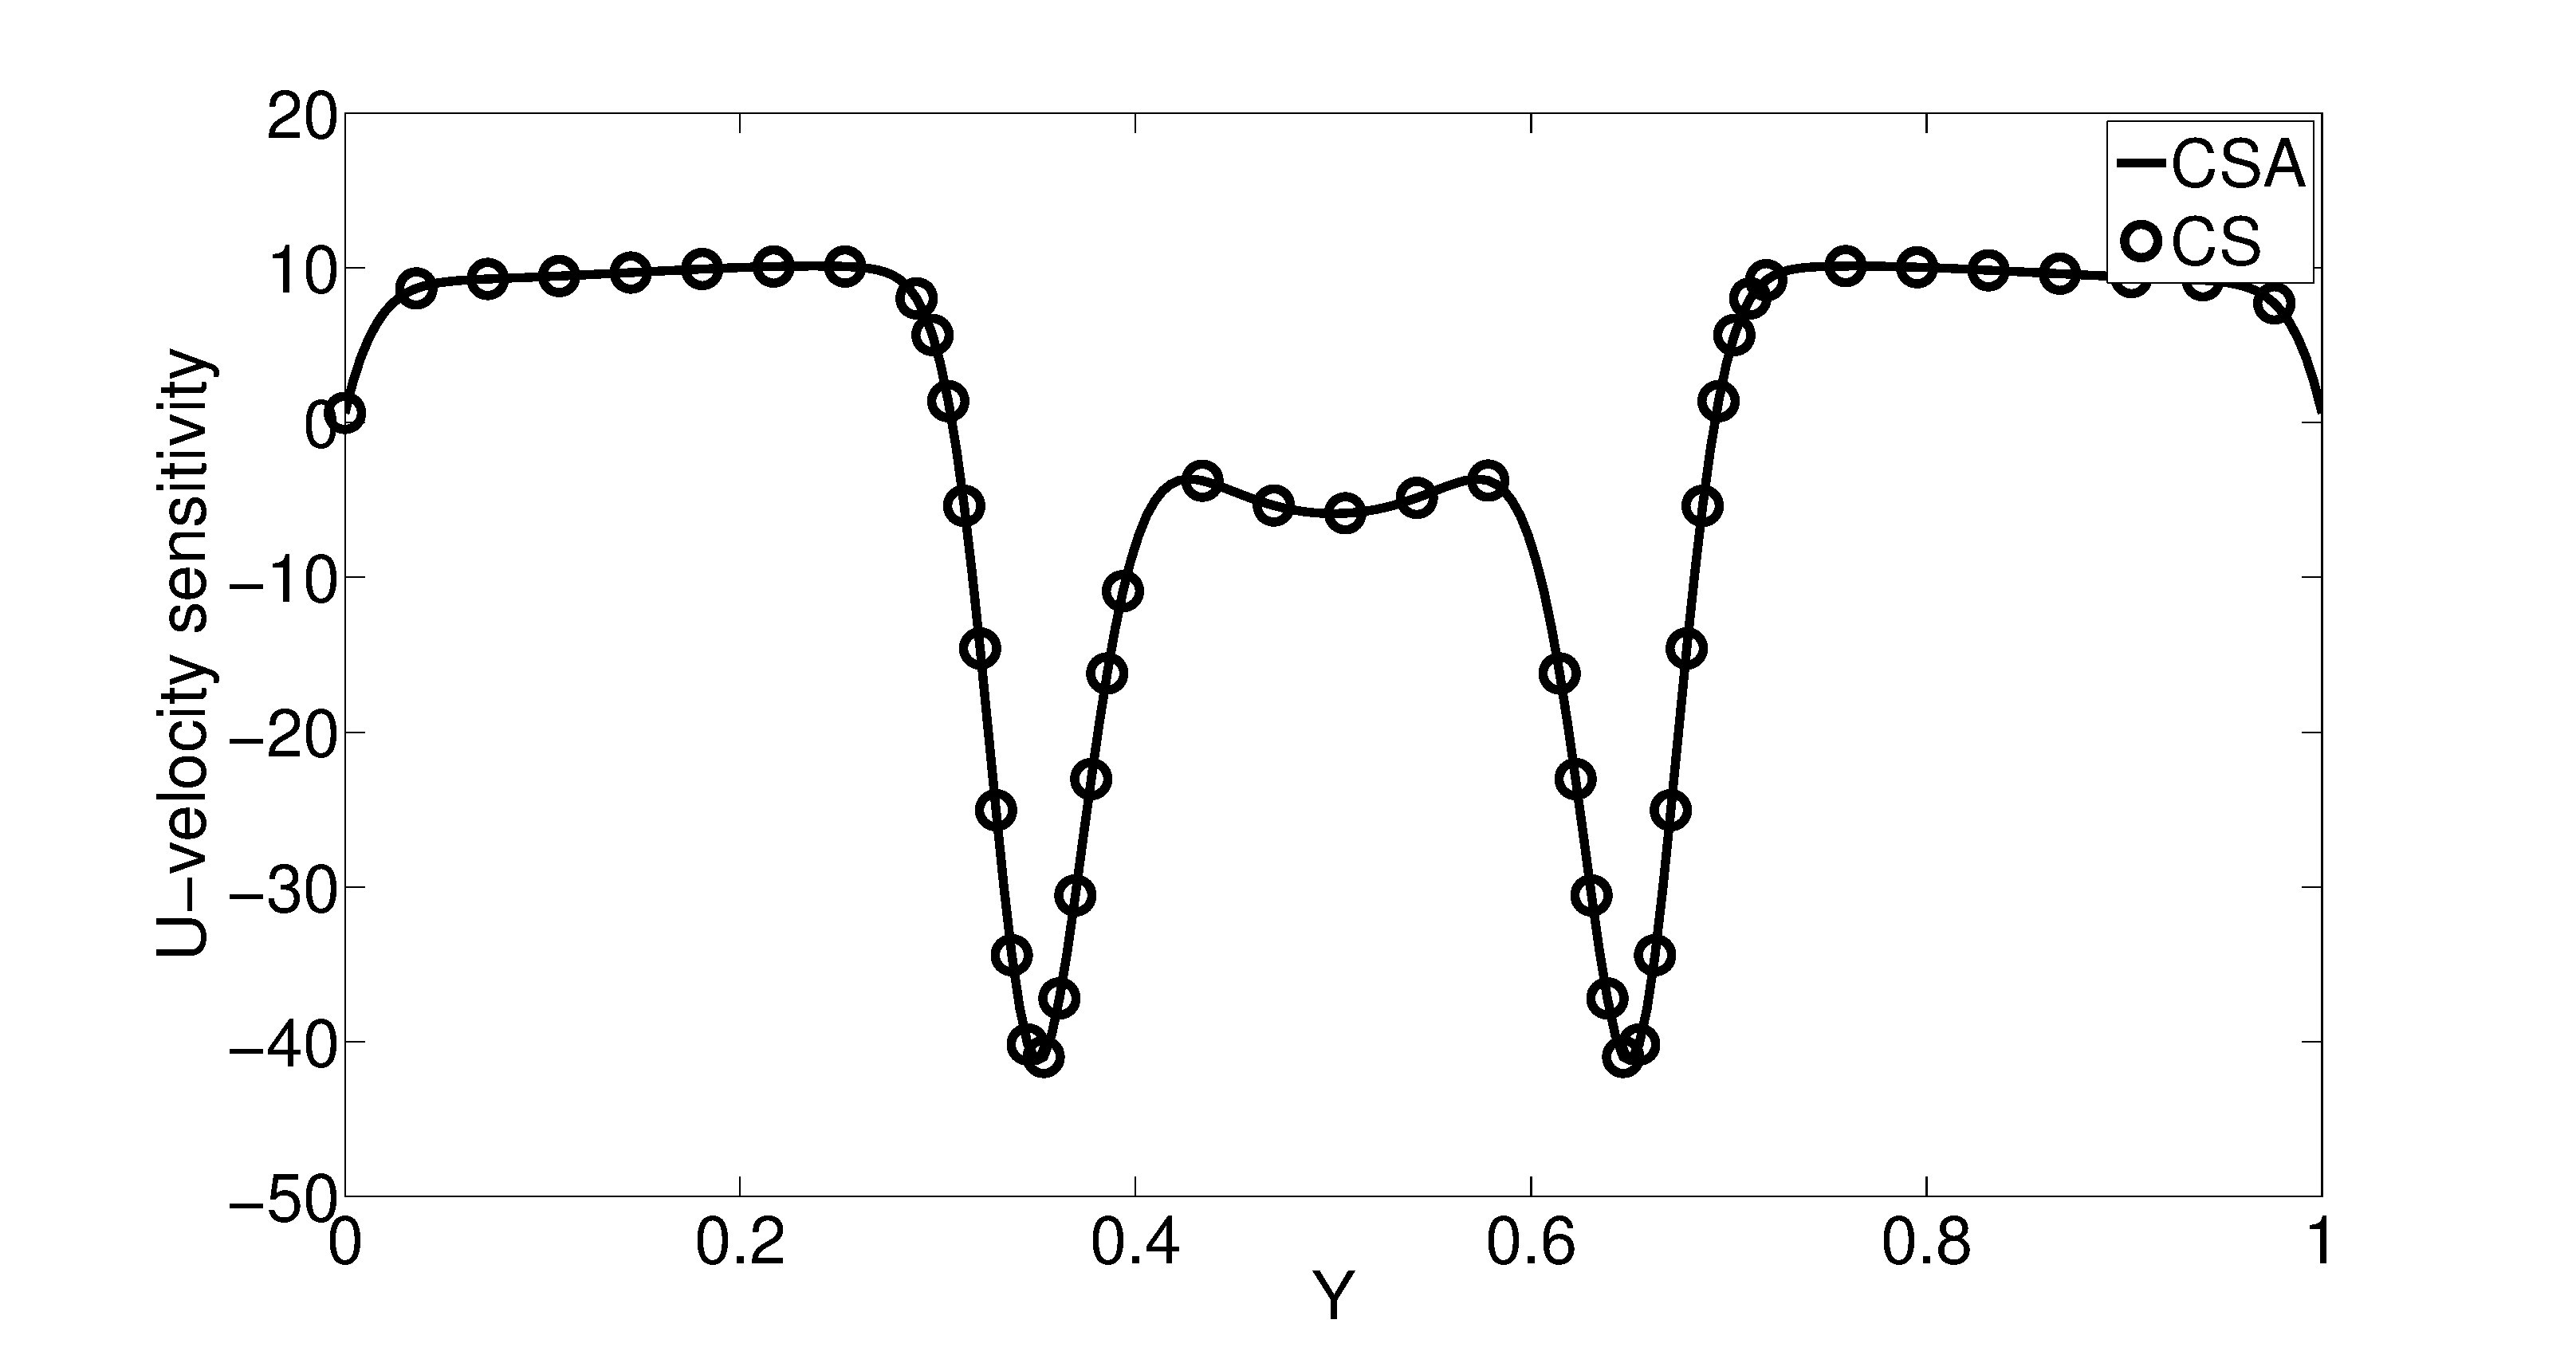
\includegraphics[height=4.0cm]{figure/cylinder/Up075_RE1000.eps}
	}
	\\
	\subfigure[x = 1.00, Re = 100]
	{
	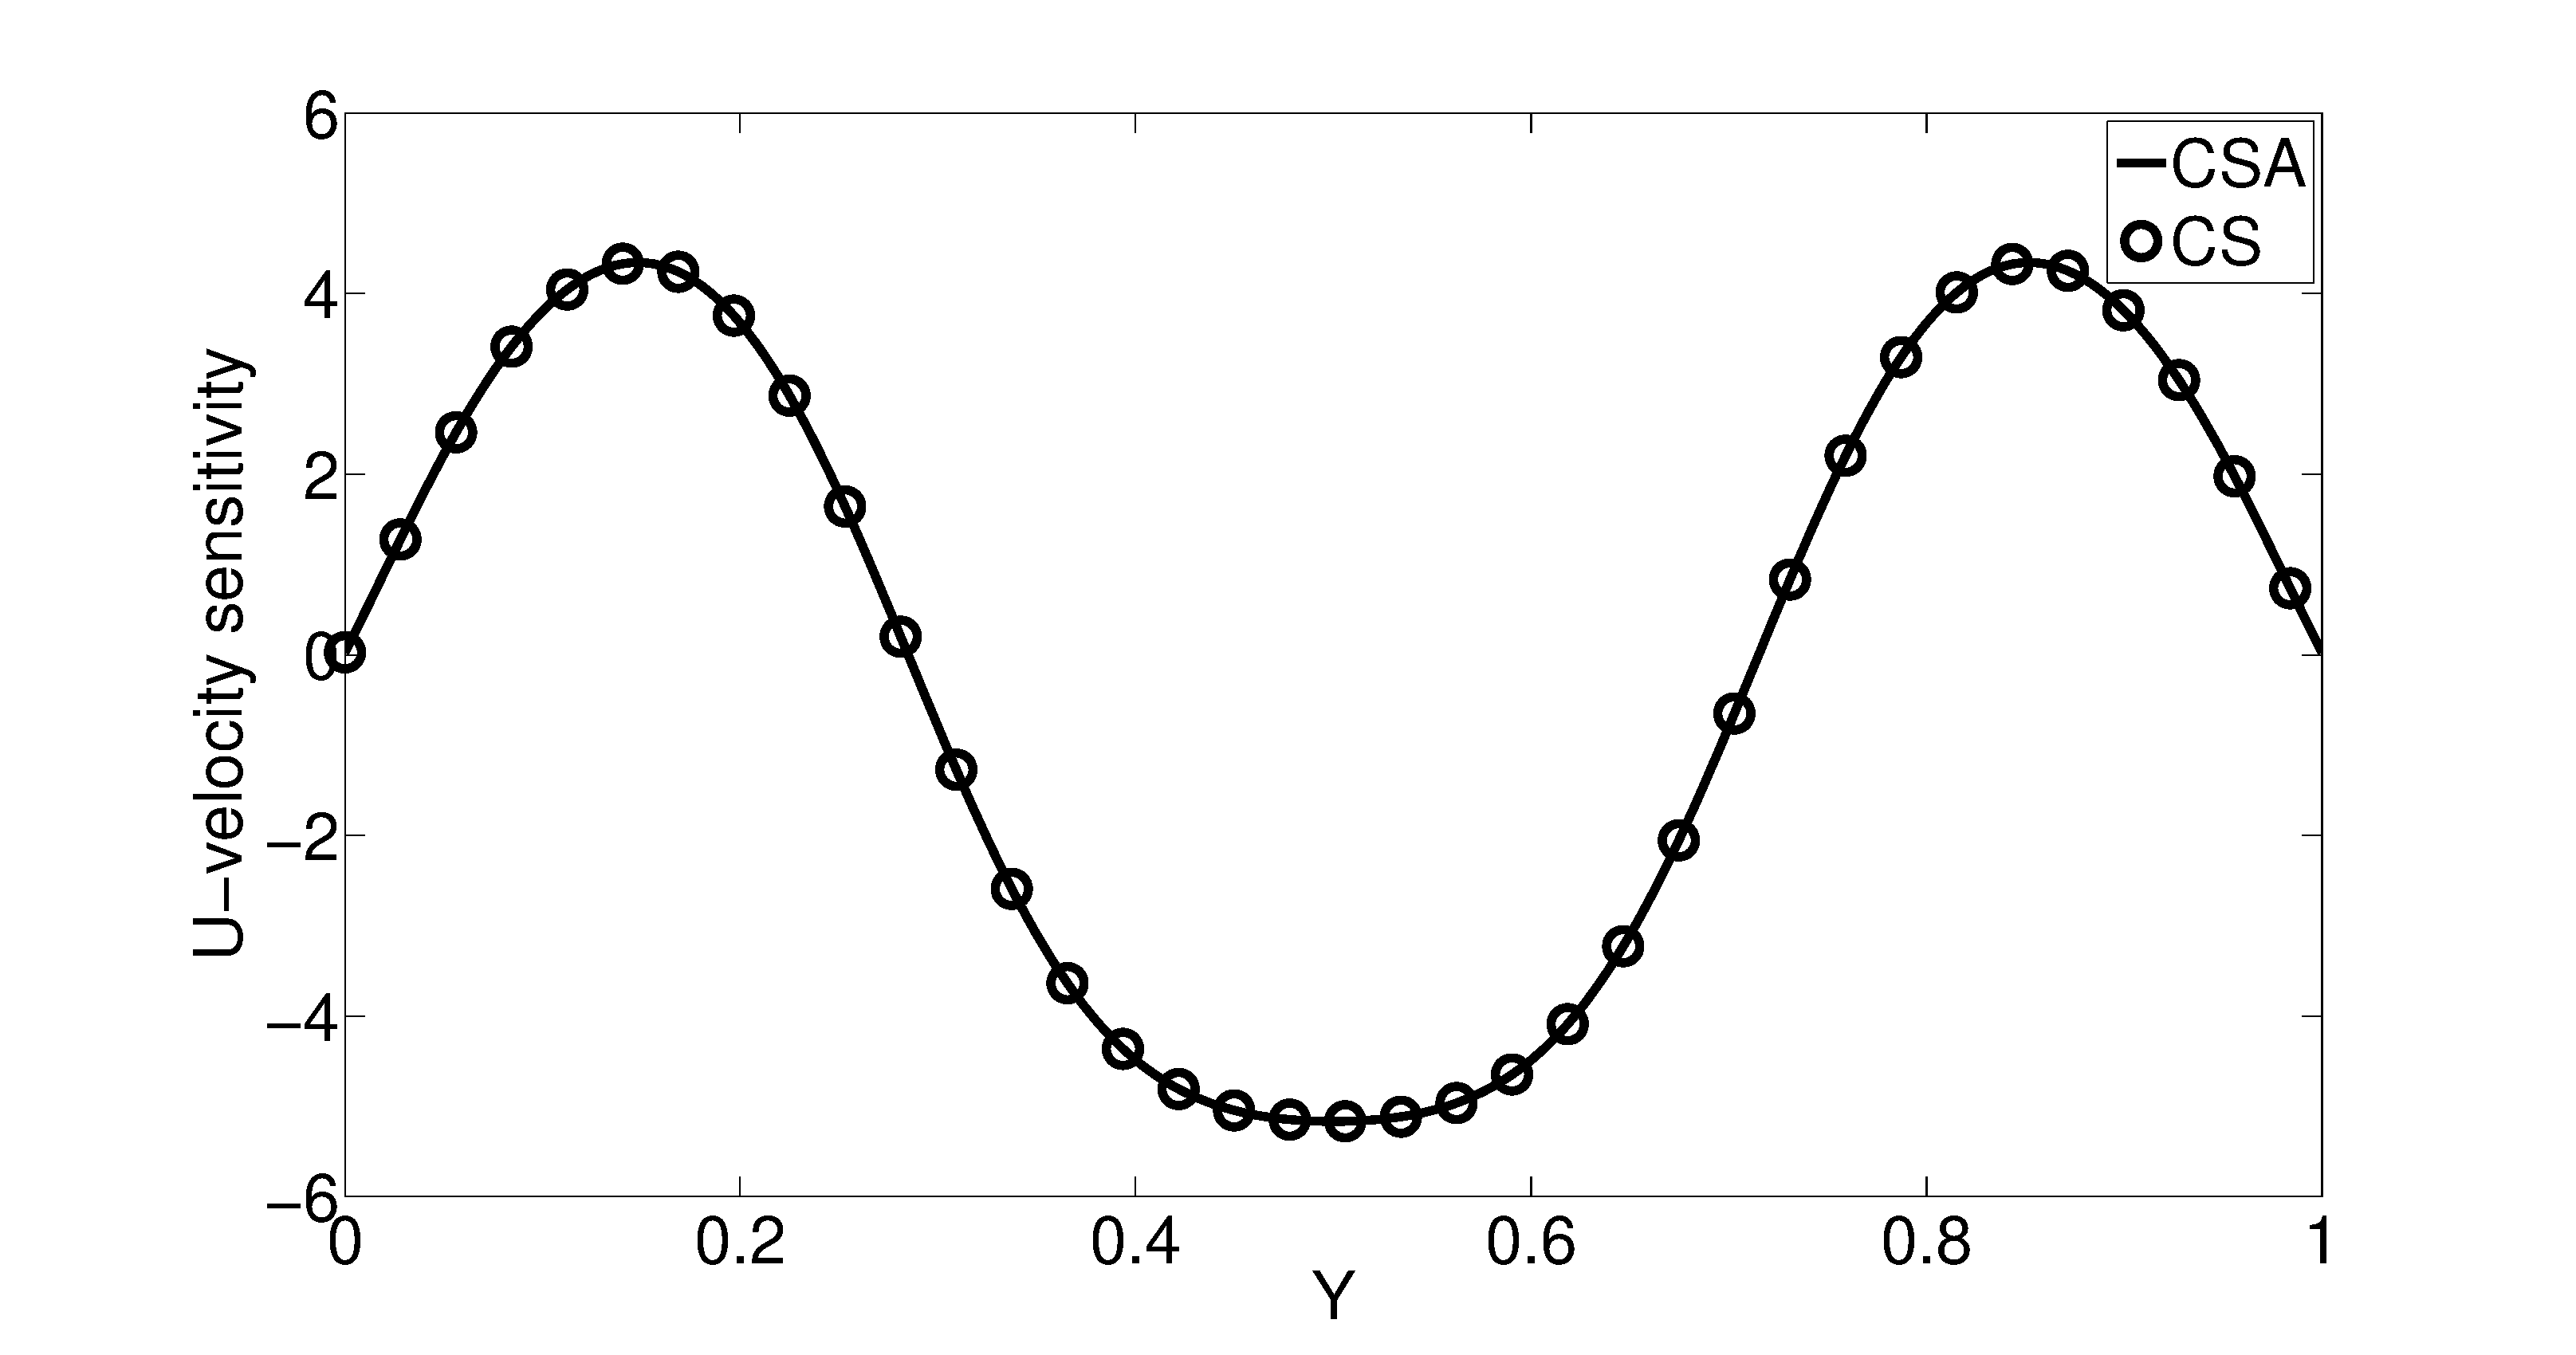
\includegraphics[height=4.0cm]{figure/cylinder/Up100_RE100.eps}
	}
	\quad
	\subfigure[x = 1.00, Re = 1000]
	{
	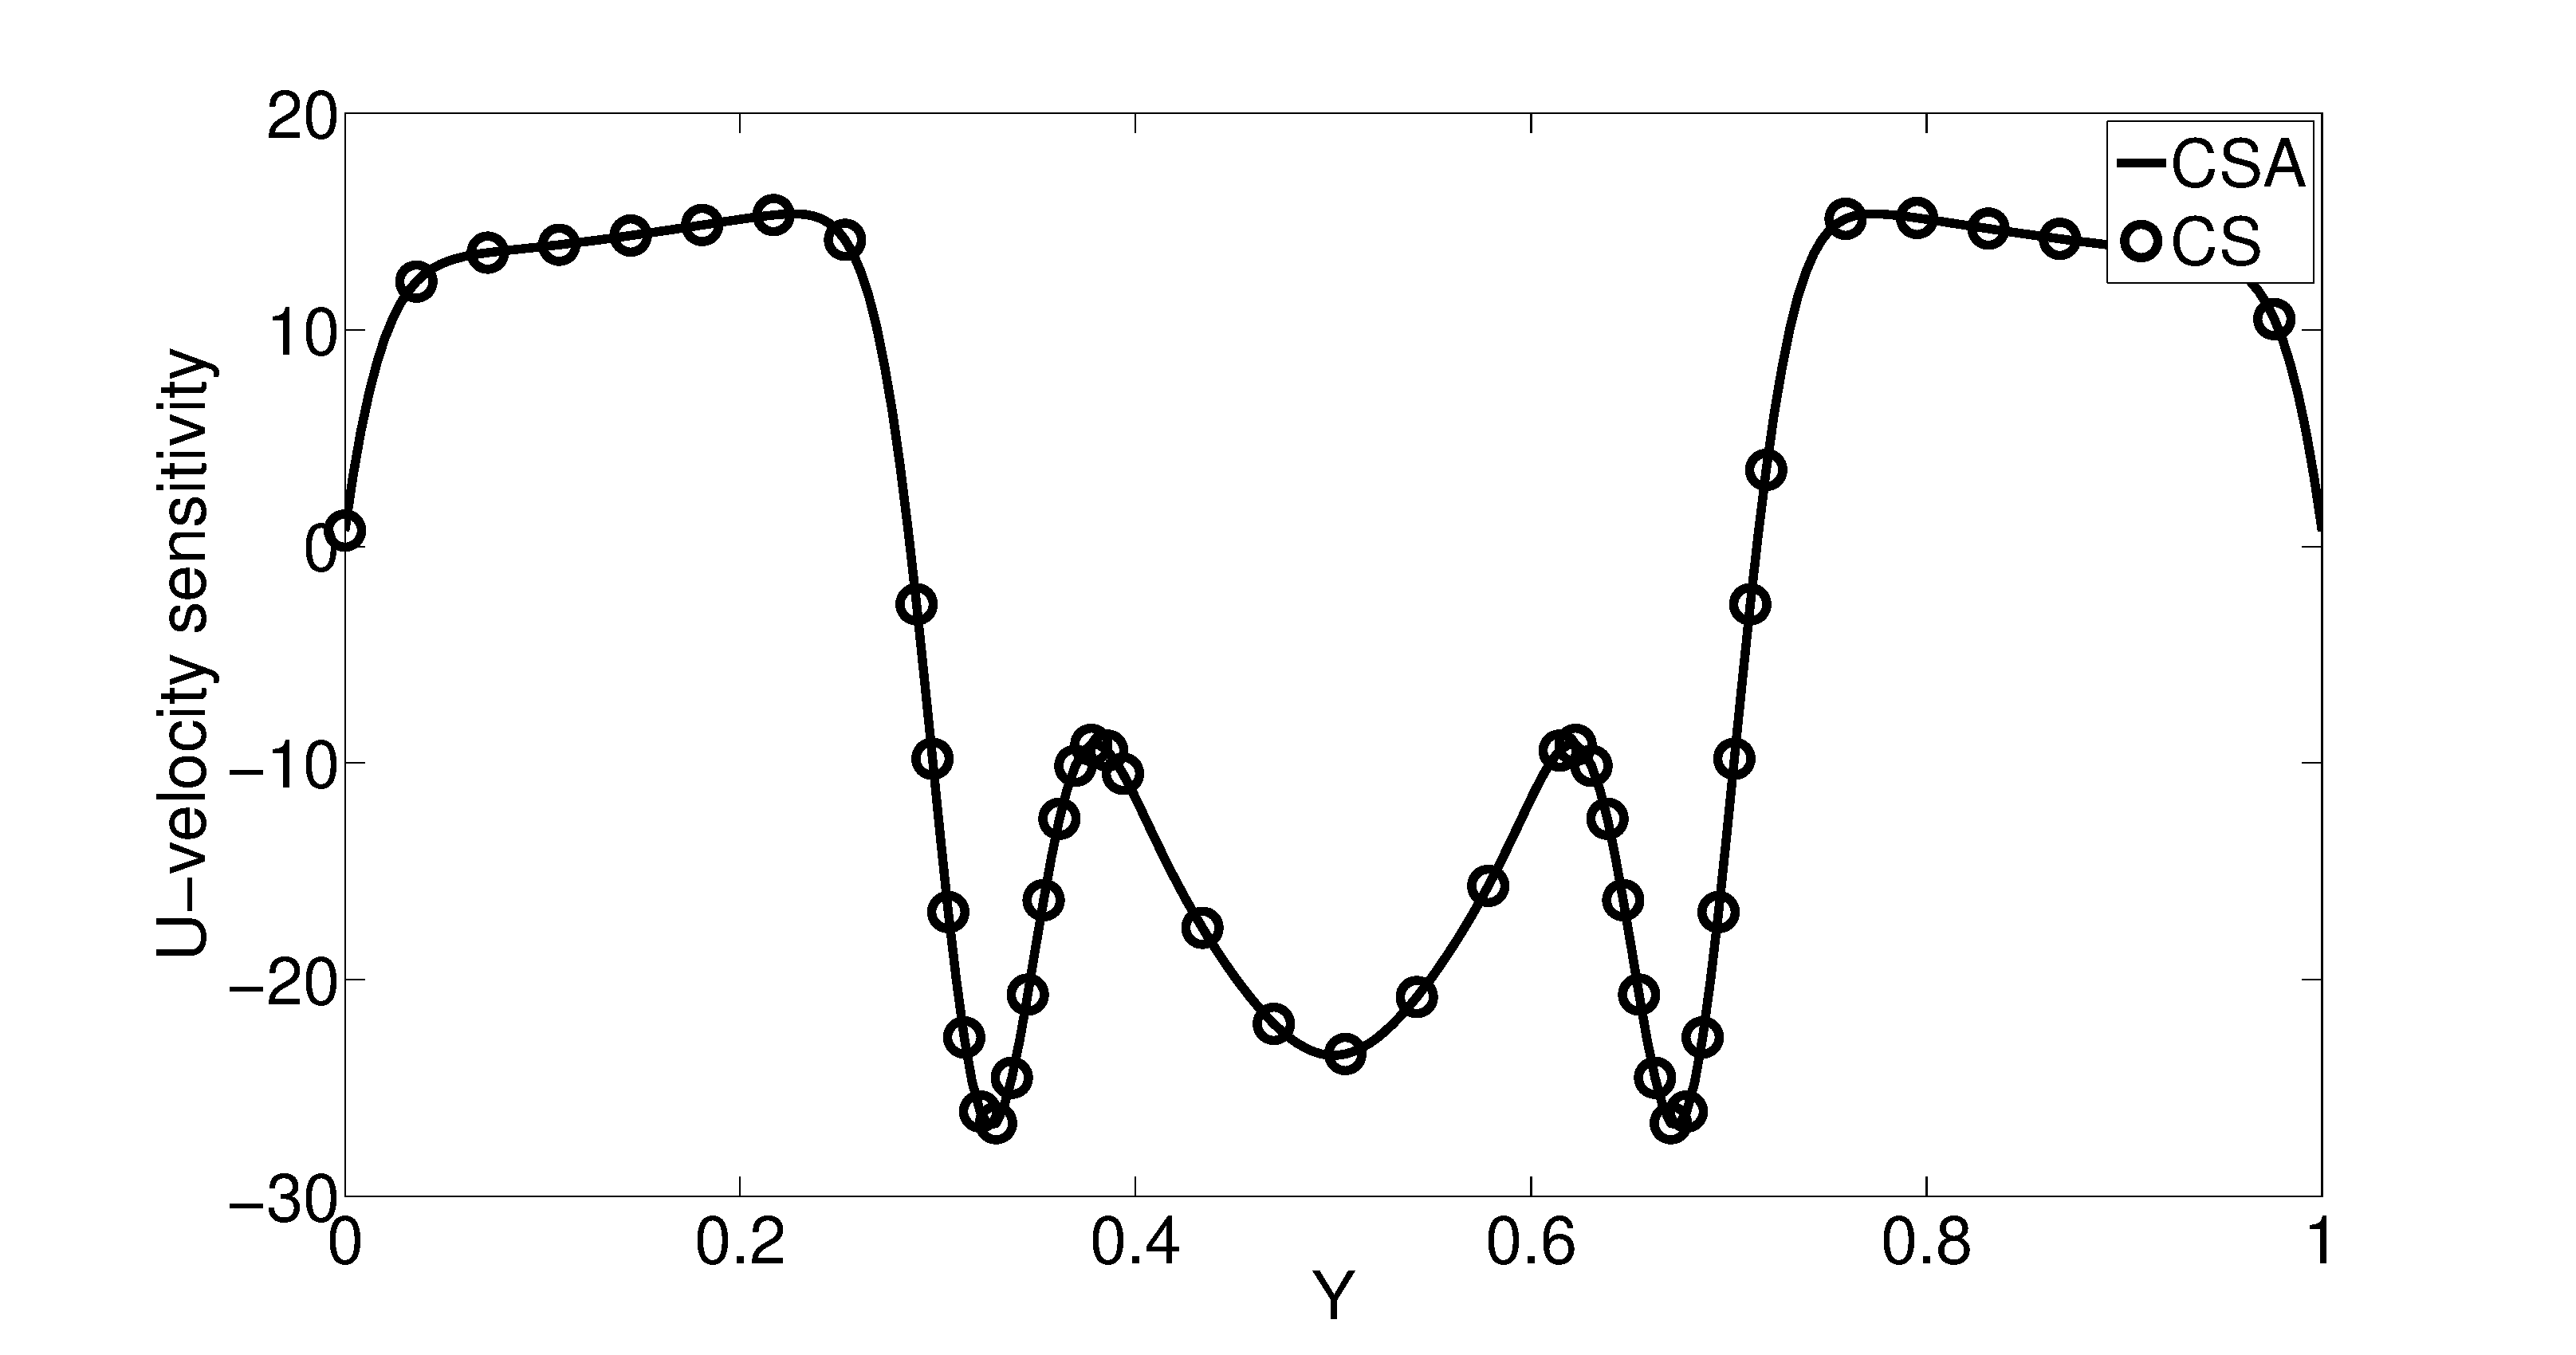
\includegraphics[height=4.0cm]{figure/cylinder/Up100_RE1000.eps}
	}
	\caption{U-velocity sensitivity to cylinder radius for different Reynolds numbers on vertical sampling line.}
	\label{fig:cylinderVelocitySensitivity}
\end{figure}
%

% -.-.-.-.-.-.-.-.-.-.-.-.-.-.-.-.-.-.-.-.-.-.-.-.-.-.-.-.-.-.-.-.-.-.-.-.-.-.-.-.-.-.-.-.-.-.-.-.-.-.-.-.-
\subsection{Linear Beam with an Airfoil}
Laminar flow over a simplified wing is selected as the second demonstration problem. The physical model for this problem is shown in Figure \ref{fig:wingModel}. The one-way fluid-solid interaction is defined by mounting the airfoil on an elastic beam where the flow field is calculated using a CFD simulation. The load and moment from the aerodynamic analysis are applied on the structure through the mounting point. The beam length is $4$ $m$, with a square cross-section with the area of $0.0001$ $m^2$, and modulus of elasticity of $80$ GPa. The initial angle of attack is selected at $2$ degrees. The fluid is modeled as laminar and incompressible flow using Navier-Stokes equations. The Reynolds number for the flow is selected as 100 for this problem. The boundary conditions are defined as the inflow velocity and zero gradient of velocity at the outlet. The top and bottom walls are modelled as free-slip boundary conditions. The structure is modelled as a linear Euler-Bernoulli beam. We are interested in calculating the sensitivity of the tip displacement of the structure to the shape of the airfoil.

%
\begin{figure}[H]
	\centering
	\subfigure[Physical domain]
	{
	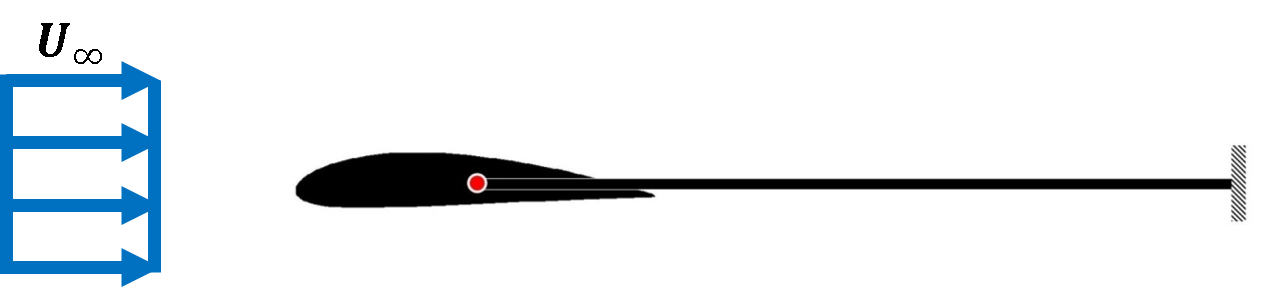
\includegraphics[width=10.0cm]{figure/airfoil/airfoil_physical_domain.png}
	}
	\\
	\subfigure[Computational domain]
	{
	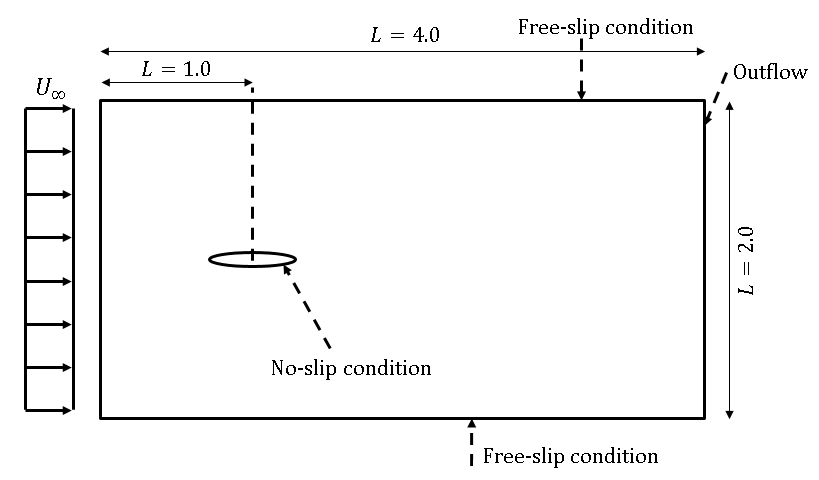
\includegraphics[width=10.0cm]{figure/airfoil/airfoil_computational_domain.png}
	}
	\caption{Simplified wing model.}
	\label{fig:wingModel}
\end{figure}
%

The airfoil is defined using the Joukowsky transformation shown in Equation \eqref{eq:joukowskyTransform}. This transformation maps a circle passing through $z_1 = 1$ and containing the point $z_2 = -1$ to a curve shaped like the cross section of an airplane wing. The Joukowsky transformation is done in a complex plane.

%
\begin{equation}\label{eq:joukowskyTransform}
J(z) = z + \frac{1}{z} \quad , \quad z = x + iy
\end{equation}
%

By changing the center location of the original circle, it is possible to change the airfoil camber. The effect of change in the center location of the original circle on the camber and thickness of the airfoil is shown in Figure \ref{fig:joukowskiChamber}. It should be noted that after geometry generation, the airfoils are normalized such that the chord length is always equal to one.\\

%
	\begin{figure}[H]
		\centering
		\subfigure[Original circle at $(-0.1,0.1)$]
		{
		\includegraphics[height=4cm]{figure/airfoil/airfoil1_shape.eps}
		\label{fig:joukowskiChamber_A}
		}
		\quad
		\subfigure[Original circle at $(-0.05,0.3)$]
		{
		\includegraphics[height=4cm]{figure/airfoil/airfoil2_shape.eps}
		\label{fig:joukowskiChamber_B}
		}
		\caption{Airfoil definition by Joukowsky transformation (not normalized).}
		\label{fig:joukowskiChamber}
	\end{figure}
%

The pressure and u-velocity contour plots for the flow over the airfoils are shown in Figure \ref{fig:flowOverAirfoil}. We refer to the airfoil shown in Figure \ref{fig:joukowskiChamber_A} as $J_1$ and Figure \ref{fig:joukowskiChamber_B} as $J_2$.

%
	\begin{figure}[H]
		\centering
		\subfigure[Pressure contour]
		{
		\includegraphics[height=4cm]{figure/airfoil/airfoil1_P.png}
		}
		\quad
		\subfigure[Pressure contour]
		{
		\includegraphics[height=4cm]{figure/airfoil/airfoil2_P.png}
		}
		\\
		\subfigure[Velocity contour]
		{
		\includegraphics[height=4cm]{figure/airfoil/airfoil1_U.png}

		}
		\quad
		\subfigure[Velocity contour]
		{
		\includegraphics[height=4cm]{figure/airfoil/airfoil2_U.png}
		}
		\caption{Airfoil definition by Joukowsky transformation (not normalized).}
		\label{fig:flowOverAirfoil}
	\end{figure}
%

The governing equations, along with the boundary conditions, are differentiated to derive the CSEs as described in the previous section. The resulting system of equations is solved to get the sensitivity response of the system. As shown in Figure \ref{fig:joukowskiChamber}, the $y$ coordinate of the center of the original circle defines the camber. The tip displacement is proportional to the load on the structure, which itself depends on the integral of the pressure over the surface of the airfoil. Therefore, to calculate the tip displacement sensitivity, one must calculate calculate the pressure sensitivity and integrate it over the airfoil boundary.

The pressure field sensitivity on the top and bottom surfaces of the airfoil to camber line variation is shown in Figure \ref{fig:joukowskiChamberSensitivity}.

%
	\begin{figure}[H]
		\centering
		\subfigure[$J_1$ airfoil]
		{
		\includegraphics[height=4.15cm]{figure/airfoil/airfoil1.eps}
		}
		\quad
		\subfigure[$J_2$ airfoil]
		{
		\includegraphics[height=4.15cm]{figure/airfoil/airfoil2.eps}
		}
		\caption{Pressure sensitivity on the surface of the airfoils.}
		\label{fig:joukowskiChamberSensitivity}
	\end{figure}
%

The integral of these functions are used to calculate the sensitivity of lift, drag, and pitching moment of the airfoil to the change in its camber. Moreover, the sensitivity of pressure field is utilized to calculate the sensitivity of tip displacement to the change in airfoil camber. We were able to match the continuum sensitivity analysis results with the complex step method. These results for two different airfoils are shown in Table \ref{table:sensitivity} where $L$ is lift force, $D$ is drag force, $M_c$ is pitching moment, and $\delta$ is the tip displacement.

%
\begin{table}[H]
\centering
\begin{tabular}{c|c|c}
 & \multicolumn{2}{c}{Airfoil} \\ \cline{2-3}
 & $J_1$ & $J_2$ \\ \hline \hline
$dL/dy_c$ & 4.839 & 7.44 \\ \hline
$dD/dy_c$ & 1.752 & 2.748 \\ \hline
$dM_c/dy_c$ & 2.481 & 3.828 \\ \hline
$d\delta/dy_c$ & 0.441 & 0.68 \\ \hline
\end{tabular}
\caption{Sensitivity results.}
\label{table:sensitivity}
\end{table}
%

% ==========================================================================================
\section{Summary Remarks}
In this research, a continuum sensitivity analysis formulation is developed for the shape sensitivity analysis for fluid-solid interaction problems. The flow is modelled with the incompressible Navier-Stokes equations. The solid boundaries are modelled using the continuum formulation of immersed boundary method with an addition of feedback forcing function in the Navier-Stokes equations to represent the effect of solid boundaries. Using this approach, we were able to decouple the fluid mesh description from the shape of the solid boundary. This approach improves the robustness of the coupled high-fidelity simulations since no mesh deformation is needed to handle the solid region deformation. Moreover, the sensitivity analysis is simplified since the local and total sensitivities are equal for this formulation. A nonlinear mapping function is used to couple the fluid and solid domain (Eulerian and Lagrangian) grids and map the data between these domains. As a requirement for continuum sensitivity analysis, the mapping function need to be $\mathcal{C}^1$ continuous. This is satisfied by proposing a novel regularized delta function that has continuous derivatives. The applicability of the proposed function is showed in this research.

The sensitivity analysis methodology is applied to two different demonstration problems. For the first problem, the flow sensitivity to the radius of an immersed cylinder is calculated. The results conform well with the complex step results. It was shown that the method can handle flow with different Reynolds numbers. For the second demonstration problem, the one-way coupling of structural response and the fluid domain is investigated. The tip displacement sensitivity of the simplified wing model to the shape of the lifting surface is calculated and the results demonstrated the accuracy.
% ==========================================================================================
\section*{Acknowledgements}
The authors would like to acknowledge the support provided by the Air Force Research Laboratory through the contract FA8650-09-23938, the Collaborative Center for Multidisciplinary Sciences.
% References
\bibliographystyle{aiaa}
\bibliography{ref}


\end{document}